\documentclass[twoside]{book}

% Packages required by doxygen
\usepackage{fixltx2e}
\usepackage{calc}
\usepackage{doxygen}
\usepackage[export]{adjustbox} % also loads graphicx
\usepackage{graphicx}
\usepackage[utf8]{inputenc}
\usepackage{makeidx}
\usepackage{multicol}
\usepackage{multirow}
\PassOptionsToPackage{warn}{textcomp}
\usepackage{textcomp}
\usepackage[nointegrals]{wasysym}
\usepackage[table]{xcolor}

% Font selection
\usepackage[T1]{fontenc}
\usepackage[scaled=.90]{helvet}
\usepackage{courier}
\usepackage{amssymb}
\usepackage{sectsty}
\renewcommand{\familydefault}{\sfdefault}
\allsectionsfont{%
  \fontseries{bc}\selectfont%
  \color{darkgray}%
}
\renewcommand{\DoxyLabelFont}{%
  \fontseries{bc}\selectfont%
  \color{darkgray}%
}
\newcommand{\+}{\discretionary{\mbox{\scriptsize$\hookleftarrow$}}{}{}}

% Page & text layout
\usepackage{geometry}
\geometry{%
  a4paper,%
  top=2.5cm,%
  bottom=2.5cm,%
  left=2.5cm,%
  right=2.5cm%
}
\tolerance=750
\hfuzz=15pt
\hbadness=750
\setlength{\emergencystretch}{15pt}
\setlength{\parindent}{0cm}
\setlength{\parskip}{3ex plus 2ex minus 2ex}
\makeatletter
\renewcommand{\paragraph}{%
  \@startsection{paragraph}{4}{0ex}{-1.0ex}{1.0ex}{%
    \normalfont\normalsize\bfseries\SS@parafont%
  }%
}
\renewcommand{\subparagraph}{%
  \@startsection{subparagraph}{5}{0ex}{-1.0ex}{1.0ex}{%
    \normalfont\normalsize\bfseries\SS@subparafont%
  }%
}
\makeatother

% Headers & footers
\usepackage{fancyhdr}
\pagestyle{fancyplain}
\fancyhead[LE]{\fancyplain{}{\bfseries\thepage}}
\fancyhead[CE]{\fancyplain{}{}}
\fancyhead[RE]{\fancyplain{}{\bfseries\leftmark}}
\fancyhead[LO]{\fancyplain{}{\bfseries\rightmark}}
\fancyhead[CO]{\fancyplain{}{}}
\fancyhead[RO]{\fancyplain{}{\bfseries\thepage}}
\fancyfoot[LE]{\fancyplain{}{}}
\fancyfoot[CE]{\fancyplain{}{}}
\fancyfoot[RE]{\fancyplain{}{\bfseries\scriptsize Generated by Doxygen }}
\fancyfoot[LO]{\fancyplain{}{\bfseries\scriptsize Generated by Doxygen }}
\fancyfoot[CO]{\fancyplain{}{}}
\fancyfoot[RO]{\fancyplain{}{}}
\renewcommand{\footrulewidth}{0.4pt}
\renewcommand{\chaptermark}[1]{%
  \markboth{#1}{}%
}
\renewcommand{\sectionmark}[1]{%
  \markright{\thesection\ #1}%
}

% Indices & bibliography
\usepackage{natbib}
\usepackage[titles]{tocloft}
\setcounter{tocdepth}{3}
\setcounter{secnumdepth}{5}
\makeindex

% Hyperlinks (required, but should be loaded last)
\usepackage{ifpdf}
\ifpdf
  \usepackage[pdftex,pagebackref=true]{hyperref}
\else
  \usepackage[ps2pdf,pagebackref=true]{hyperref}
\fi
\hypersetup{%
  colorlinks=true,%
  linkcolor=blue,%
  citecolor=blue,%
  unicode%
}

% Custom commands
\newcommand{\clearemptydoublepage}{%
  \newpage{\pagestyle{empty}\cleardoublepage}%
}

\usepackage{caption}
\captionsetup{labelsep=space,justification=centering,font={bf},singlelinecheck=off,skip=4pt,position=top}

%===== C O N T E N T S =====

\begin{document}

% Titlepage & ToC
\hypersetup{pageanchor=false,
             bookmarksnumbered=true,
             pdfencoding=unicode
            }
\pagenumbering{alph}
\begin{titlepage}
\vspace*{7cm}
\begin{center}%
{\Large My Project }\\
\vspace*{1cm}
{\large Generated by Doxygen 1.8.13}\\
\end{center}
\end{titlepage}
\clearemptydoublepage
\pagenumbering{roman}
\tableofcontents
\clearemptydoublepage
\pagenumbering{arabic}
\hypersetup{pageanchor=true}

%--- Begin generated contents ---
\chapter{R\+T2D -\/ 2D Open\+GL Framework}
\label{index}\hypertarget{index}{}\hypertarget{index_intro}{}\section{Introduction}\label{index_intro}
R\+T2D is a Real\+Time 2D framework, based on \textquotesingle{}modern\textquotesingle{} Open\+GL (2.\+1+). It runs on Mac, Linux and Windows.

Please see {\ttfamily R\+E\+A\+D\+M\+E.\+md} for instructions on compiling for your platform of choice.\hypertarget{index_license}{}\section{License}\label{index_license}
Copyright 2015 Rik Teerling \href{mailto:rik@onandoffables.com}{\tt rik@onandoffables.\+com}

This program is free software; you can redistribute it and/or modify it under the terms of the G\+NU General Public License as published by the Free Software Foundation; either version 2 of the License, or (at your option) any later version.

This program is distributed in the hope that it will be useful, but W\+I\+T\+H\+O\+UT A\+NY W\+A\+R\+R\+A\+N\+TY; without even the implied warranty of M\+E\+R\+C\+H\+A\+N\+T\+A\+B\+I\+L\+I\+TY or F\+I\+T\+N\+E\+SS F\+OR A P\+A\+R\+T\+I\+C\+U\+L\+AR P\+U\+R\+P\+O\+SE. See the G\+NU General Public License for more details.

You should have received a copy of the G\+NU General Public License along with this program; if not, write to the Free Software Foundation, Inc., 51 Franklin Street, Fifth Floor, Boston, MA 02110-\/1301, U\+SA. 
\chapter{Hierarchical Index}
\section{Class Hierarchy}
This inheritance list is sorted roughly, but not completely, alphabetically\+:\begin{DoxyCompactList}
\item \contentsline{section}{Block}{\pageref{struct_block}}{}
\item \contentsline{section}{Boid}{\pageref{class_boid}}{}
\item \contentsline{section}{Cell}{\pageref{struct_cell}}{}
\item Entity\begin{DoxyCompactList}
\item \contentsline{section}{Basic\+Entity}{\pageref{class_basic_entity}}{}
\item \contentsline{section}{Canvas}{\pageref{class_canvas}}{}
\item \contentsline{section}{Hex\+Field}{\pageref{struct_hex_field}}{}
\end{DoxyCompactList}
\item \contentsline{section}{Field}{\pageref{struct_field}}{}
\item \contentsline{section}{Particle}{\pageref{struct_particle}}{}
\item \contentsline{section}{Pixel}{\pageref{struct_pixel}}{}
\item \contentsline{section}{Pixel\+Sprite}{\pageref{struct_pixel_sprite}}{}
\item \contentsline{section}{Player}{\pageref{struct_player}}{}
\item Scene\begin{DoxyCompactList}
\item \contentsline{section}{Super\+Scene}{\pageref{class_super_scene}}{}
\begin{DoxyCompactList}
\item \contentsline{section}{Scene00}{\pageref{class_scene00}}{}
\item \contentsline{section}{Scene01}{\pageref{class_scene01}}{}
\item \contentsline{section}{Scene02}{\pageref{class_scene02}}{}
\item \contentsline{section}{Scene03}{\pageref{class_scene03}}{}
\item \contentsline{section}{Scene03a}{\pageref{class_scene03a}}{}
\item \contentsline{section}{Scene03b}{\pageref{class_scene03b}}{}
\item \contentsline{section}{Scene04}{\pageref{class_scene04}}{}
\item \contentsline{section}{Scene05}{\pageref{class_scene05}}{}
\item \contentsline{section}{Scene06}{\pageref{class_scene06}}{}
\item \contentsline{section}{Scene06a}{\pageref{class_scene06a}}{}
\item \contentsline{section}{Scene07}{\pageref{class_scene07}}{}
\item \contentsline{section}{Scene08}{\pageref{class_scene08}}{}
\item \contentsline{section}{Scene09}{\pageref{class_scene09}}{}
\item \contentsline{section}{Scene10}{\pageref{class_scene10}}{}
\item \contentsline{section}{Scene11}{\pageref{class_scene11}}{}
\item \contentsline{section}{Scene12}{\pageref{class_scene12}}{}
\item \contentsline{section}{Scene13}{\pageref{class_scene13}}{}
\item \contentsline{section}{Scene14}{\pageref{class_scene14}}{}
\item \contentsline{section}{Scene15}{\pageref{class_scene15}}{}
\end{DoxyCompactList}
\end{DoxyCompactList}
\item \contentsline{section}{S\+I\+\_\+\+Animated\+Sprite}{\pageref{struct_s_i___animated_sprite}}{}
\end{DoxyCompactList}

\chapter{Class Index}
\section{Class List}
Here are the classes, structs, unions and interfaces with brief descriptions\+:\begin{DoxyCompactList}
\item\contentsline{section}{\hyperlink{class_basic_entity}{Basic\+Entity} }{\pageref{class_basic_entity}}{}
\item\contentsline{section}{\hyperlink{struct_block}{Block} }{\pageref{struct_block}}{}
\item\contentsline{section}{\hyperlink{class_boid}{Boid} }{\pageref{class_boid}}{}
\item\contentsline{section}{\hyperlink{class_canvas}{Canvas} }{\pageref{class_canvas}}{}
\item\contentsline{section}{\hyperlink{struct_cell}{Cell} }{\pageref{struct_cell}}{}
\item\contentsline{section}{\hyperlink{struct_field}{Field} }{\pageref{struct_field}}{}
\item\contentsline{section}{\hyperlink{struct_hex_field}{Hex\+Field} }{\pageref{struct_hex_field}}{}
\item\contentsline{section}{\hyperlink{struct_particle}{Particle} }{\pageref{struct_particle}}{}
\item\contentsline{section}{\hyperlink{struct_pixel}{Pixel} }{\pageref{struct_pixel}}{}
\item\contentsline{section}{\hyperlink{struct_pixel_sprite}{Pixel\+Sprite} }{\pageref{struct_pixel_sprite}}{}
\item\contentsline{section}{\hyperlink{struct_player}{Player} }{\pageref{struct_player}}{}
\item\contentsline{section}{\hyperlink{class_scene00}{Scene00} }{\pageref{class_scene00}}{}
\item\contentsline{section}{\hyperlink{class_scene01}{Scene01} }{\pageref{class_scene01}}{}
\item\contentsline{section}{\hyperlink{class_scene02}{Scene02} }{\pageref{class_scene02}}{}
\item\contentsline{section}{\hyperlink{class_scene03}{Scene03} }{\pageref{class_scene03}}{}
\item\contentsline{section}{\hyperlink{class_scene03a}{Scene03a} }{\pageref{class_scene03a}}{}
\item\contentsline{section}{\hyperlink{class_scene03b}{Scene03b} }{\pageref{class_scene03b}}{}
\item\contentsline{section}{\hyperlink{class_scene04}{Scene04} }{\pageref{class_scene04}}{}
\item\contentsline{section}{\hyperlink{class_scene05}{Scene05} }{\pageref{class_scene05}}{}
\item\contentsline{section}{\hyperlink{class_scene06}{Scene06} }{\pageref{class_scene06}}{}
\item\contentsline{section}{\hyperlink{class_scene06a}{Scene06a} }{\pageref{class_scene06a}}{}
\item\contentsline{section}{\hyperlink{class_scene07}{Scene07} }{\pageref{class_scene07}}{}
\item\contentsline{section}{\hyperlink{class_scene08}{Scene08} }{\pageref{class_scene08}}{}
\item\contentsline{section}{\hyperlink{class_scene09}{Scene09} }{\pageref{class_scene09}}{}
\item\contentsline{section}{\hyperlink{class_scene10}{Scene10} }{\pageref{class_scene10}}{}
\item\contentsline{section}{\hyperlink{class_scene11}{Scene11} }{\pageref{class_scene11}}{}
\item\contentsline{section}{\hyperlink{class_scene12}{Scene12} }{\pageref{class_scene12}}{}
\item\contentsline{section}{\hyperlink{class_scene13}{Scene13} }{\pageref{class_scene13}}{}
\item\contentsline{section}{\hyperlink{class_scene14}{Scene14} }{\pageref{class_scene14}}{}
\item\contentsline{section}{\hyperlink{class_scene15}{Scene15} }{\pageref{class_scene15}}{}
\item\contentsline{section}{\hyperlink{struct_s_i___animated_sprite}{S\+I\+\_\+\+Animated\+Sprite} }{\pageref{struct_s_i___animated_sprite}}{}
\item\contentsline{section}{\hyperlink{class_super_scene}{Super\+Scene} }{\pageref{class_super_scene}}{}
\end{DoxyCompactList}

\chapter{File Index}
\section{File List}
Here is a list of all documented files with brief descriptions\+:\begin{DoxyCompactList}
\item\contentsline{section}{\hyperlink{camera_8h}{camera.\+h} \\*The \hyperlink{class_camera}{Camera} header file }{\pageref{camera_8h}}{}
\item\contentsline{section}{\hyperlink{color_8h}{color.\+h} \\*The \hyperlink{struct_color}{Color} header file }{\pageref{color_8h}}{}
\item\contentsline{section}{\hyperlink{core_8h}{core.\+h} \\*The \hyperlink{class_core}{Core} header file }{\pageref{core_8h}}{}
\item\contentsline{section}{\hyperlink{entity_8h}{entity.\+h} \\*The \hyperlink{class_entity}{Entity} header file }{\pageref{entity_8h}}{}
\item\contentsline{section}{\hyperlink{input_8h}{input.\+h} \\*The \hyperlink{class_input}{Input} header file }{\pageref{input_8h}}{}
\item\contentsline{section}{\hyperlink{line_8h}{line.\+h} \\*The \hyperlink{class_line}{Line} header file }{\pageref{line_8h}}{}
\item\contentsline{section}{\hyperlink{mesh_8h}{mesh.\+h} \\*The \hyperlink{class_mesh}{Mesh} header file }{\pageref{mesh_8h}}{}
\item\contentsline{section}{\hyperlink{noise_8h}{noise.\+h} \\*The \hyperlink{class_noise}{Noise} header file }{\pageref{noise_8h}}{}
\item\contentsline{section}{\hyperlink{pointx_8h}{pointx.\+h} \\*The \hyperlink{class_point__t}{Point\+\_\+t} header file }{\pageref{pointx_8h}}{}
\item\contentsline{section}{\hyperlink{renderer_8h}{renderer.\+h} \\*The \hyperlink{class_renderer}{Renderer} header file }{\pageref{renderer_8h}}{}
\item\contentsline{section}{\hyperlink{resourcemanager_8h}{resourcemanager.\+h} \\*The \hyperlink{class_resource_manager}{Resource\+Manager} header file }{\pageref{resourcemanager_8h}}{}
\item\contentsline{section}{\hyperlink{rt2dconfig_8h}{rt2dconfig.\+h} \\*This header file defines some global vars }{\pageref{rt2dconfig_8h}}{}
\item\contentsline{section}{\hyperlink{scene_8h}{scene.\+h} \\*The \hyperlink{class_scene}{Scene} header file }{\pageref{scene_8h}}{}
\item\contentsline{section}{\hyperlink{shader_8h}{shader.\+h} \\*The \hyperlink{class_shader}{Shader} header file }{\pageref{shader_8h}}{}
\item\contentsline{section}{\hyperlink{sprite_8h}{sprite.\+h} \\*The \hyperlink{class_sprite}{Sprite} header file }{\pageref{sprite_8h}}{}
\item\contentsline{section}{\hyperlink{stringutil_8h}{stringutil.\+h} \\*The stringutil header file }{\pageref{stringutil_8h}}{}
\item\contentsline{section}{\hyperlink{text_8h}{text.\+h} \\*The \hyperlink{class_text}{Text} header file }{\pageref{text_8h}}{}
\item\contentsline{section}{\hyperlink{texture_8h}{texture.\+h} \\*The \hyperlink{class_texture}{Texture} header file }{\pageref{texture_8h}}{}
\item\contentsline{section}{\hyperlink{timer_8h}{timer.\+h} \\*The \hyperlink{class_timer}{Timer} header file }{\pageref{timer_8h}}{}
\item\contentsline{section}{\hyperlink{util_8h}{util.\+h} \\*The util header file }{\pageref{util_8h}}{}
\item\contentsline{section}{\hyperlink{vectorx_8h}{vectorx.\+h} \\*The \hyperlink{class_vector_x__t}{Vector\+X\+\_\+t} header file }{\pageref{vectorx_8h}}{}
\end{DoxyCompactList}

\chapter{Class Documentation}
\hypertarget{class_camera}{}\section{Camera Class Reference}
\label{class_camera}\index{Camera@{Camera}}


The \hyperlink{class_camera}{Camera} class handles the concept of having a \hyperlink{class_camera}{Camera} in your \hyperlink{class_scene}{Scene}.  




{\ttfamily \#include $<$camera.\+h$>$}

\subsection*{Public Member Functions}
\begin{DoxyCompactItemize}
\item 
\hyperlink{class_camera_a01f94c3543f56ede7af49dc778f19331}{Camera} ()
\begin{DoxyCompactList}\small\item\em Constructor of the \hyperlink{class_camera}{Camera}. \end{DoxyCompactList}\item 
\mbox{\Hypertarget{class_camera_ad1897942d0ccf91052386388a497349f}\label{class_camera_ad1897942d0ccf91052386388a497349f}} 
virtual \hyperlink{class_camera_ad1897942d0ccf91052386388a497349f}{$\sim$\+Camera} ()
\begin{DoxyCompactList}\small\item\em Destructor of the \hyperlink{class_camera}{Camera}. \end{DoxyCompactList}\item 
virtual void \hyperlink{class_camera_ac9e359b0a6c41091a0eac46a869790bf}{update\+Camera} (float delta\+Time)
\begin{DoxyCompactList}\small\item\em updates the view\+Matrix and projection\+Matrix of the \hyperlink{class_camera}{Camera}. \end{DoxyCompactList}\item 
glm\+::mat4 \hyperlink{class_camera_aa77dcf47815f0549e40111baf0998771}{view\+Matrix} ()
\begin{DoxyCompactList}\small\item\em get the view\+Matrix of the \hyperlink{class_camera}{Camera}. \end{DoxyCompactList}\item 
glm\+::mat4 \hyperlink{class_camera_a2eca875ed162335c5c8a3907d8674716}{projection\+Matrix} ()
\begin{DoxyCompactList}\small\item\em get the projection\+Matrix of the \hyperlink{class_camera}{Camera}. \end{DoxyCompactList}\end{DoxyCompactItemize}
\subsection*{Public Attributes}
\begin{DoxyCompactItemize}
\item 
\mbox{\Hypertarget{class_camera_a57fa6dbb1aabd24b2aff6644eae36533}\label{class_camera_a57fa6dbb1aabd24b2aff6644eae36533}} 
\hyperlink{pointx_8h_a1de5e45af54f9f098e4ae388726e9677}{Point} \hyperlink{class_camera_a57fa6dbb1aabd24b2aff6644eae36533}{position}
\begin{DoxyCompactList}\small\item\em The position of the \hyperlink{class_camera}{Camera}. \end{DoxyCompactList}\end{DoxyCompactItemize}


\subsection{Detailed Description}
The \hyperlink{class_camera}{Camera} class handles the concept of having a \hyperlink{class_camera}{Camera} in your \hyperlink{class_scene}{Scene}. 

\subsection{Constructor \& Destructor Documentation}
\mbox{\Hypertarget{class_camera_a01f94c3543f56ede7af49dc778f19331}\label{class_camera_a01f94c3543f56ede7af49dc778f19331}} 
\index{Camera@{Camera}!Camera@{Camera}}
\index{Camera@{Camera}!Camera@{Camera}}
\subsubsection{\texorpdfstring{Camera()}{Camera()}}
{\footnotesize\ttfamily Camera\+::\+Camera (\begin{DoxyParamCaption}{ }\end{DoxyParamCaption})}



Constructor of the \hyperlink{class_camera}{Camera}. 

This file is part of R\+T2D, a 2D Open\+GL framework.


\begin{DoxyItemize}
\item Copyright 2015 Rik Teerling \href{mailto:rik@onandoffables.com}{\tt rik@onandoffables.\+com}
\begin{DoxyItemize}
\item Initial commit 
\end{DoxyItemize}
\end{DoxyItemize}

\subsection{Member Function Documentation}
\mbox{\Hypertarget{class_camera_a2eca875ed162335c5c8a3907d8674716}\label{class_camera_a2eca875ed162335c5c8a3907d8674716}} 
\index{Camera@{Camera}!projection\+Matrix@{projection\+Matrix}}
\index{projection\+Matrix@{projection\+Matrix}!Camera@{Camera}}
\subsubsection{\texorpdfstring{projection\+Matrix()}{projectionMatrix()}}
{\footnotesize\ttfamily glm\+::mat4 Camera\+::projection\+Matrix (\begin{DoxyParamCaption}{ }\end{DoxyParamCaption})\hspace{0.3cm}{\ttfamily [inline]}}



get the projection\+Matrix of the \hyperlink{class_camera}{Camera}. 

\begin{DoxyReturn}{Returns}
glm\+::mat4 \+\_\+projection\+Matrix 
\end{DoxyReturn}
\mbox{\Hypertarget{class_camera_ac9e359b0a6c41091a0eac46a869790bf}\label{class_camera_ac9e359b0a6c41091a0eac46a869790bf}} 
\index{Camera@{Camera}!update\+Camera@{update\+Camera}}
\index{update\+Camera@{update\+Camera}!Camera@{Camera}}
\subsubsection{\texorpdfstring{update\+Camera()}{updateCamera()}}
{\footnotesize\ttfamily void Camera\+::update\+Camera (\begin{DoxyParamCaption}\item[{float}]{delta\+Time }\end{DoxyParamCaption})\hspace{0.3cm}{\ttfamily [virtual]}}



updates the view\+Matrix and projection\+Matrix of the \hyperlink{class_camera}{Camera}. 


\begin{DoxyParams}{Parameters}
{\em delta\+Time} & The time that\textquotesingle{}s passed since the last update. \\
\hline
\end{DoxyParams}
\begin{DoxyReturn}{Returns}
void 
\end{DoxyReturn}
\mbox{\Hypertarget{class_camera_aa77dcf47815f0549e40111baf0998771}\label{class_camera_aa77dcf47815f0549e40111baf0998771}} 
\index{Camera@{Camera}!view\+Matrix@{view\+Matrix}}
\index{view\+Matrix@{view\+Matrix}!Camera@{Camera}}
\subsubsection{\texorpdfstring{view\+Matrix()}{viewMatrix()}}
{\footnotesize\ttfamily glm\+::mat4 Camera\+::view\+Matrix (\begin{DoxyParamCaption}{ }\end{DoxyParamCaption})\hspace{0.3cm}{\ttfamily [inline]}}



get the view\+Matrix of the \hyperlink{class_camera}{Camera}. 

\begin{DoxyReturn}{Returns}
glm\+::mat4 \+\_\+view\+Matrix 
\end{DoxyReturn}


The documentation for this class was generated from the following files\+:\begin{DoxyCompactItemize}
\item 
\hyperlink{camera_8h}{camera.\+h}\item 
camera.\+cpp\end{DoxyCompactItemize}

\hypertarget{struct_color}{}\section{Color Struct Reference}
\label{struct_color}\index{Color@{Color}}


H\+SV $<$-\/$>$ R\+G\+BA conversion.  




{\ttfamily \#include $<$color.\+h$>$}

\subsection*{Static Public Member Functions}
\begin{DoxyCompactItemize}
\item 
\mbox{\Hypertarget{struct_color_a484629034430390400f931b8d717a449}\label{struct_color_a484629034430390400f931b8d717a449}} 
static \hyperlink{struct_h_s_v_color}{H\+S\+V\+Color} \hyperlink{struct_color_a484629034430390400f931b8d717a449}{R\+G\+B\+A2\+H\+SV} (\hyperlink{struct_r_g_b_a_color}{R\+G\+B\+A\+Color} rgba)
\begin{DoxyCompactList}\small\item\em R\+G\+BA to H\+SV conversion. \end{DoxyCompactList}\item 
\mbox{\Hypertarget{struct_color_a960f7c7dc1d48206b0ebdaa43e344c5b}\label{struct_color_a960f7c7dc1d48206b0ebdaa43e344c5b}} 
static \hyperlink{struct_r_g_b_a_color}{R\+G\+B\+A\+Color} \hyperlink{struct_color_a960f7c7dc1d48206b0ebdaa43e344c5b}{H\+S\+V2\+R\+G\+BA} (\hyperlink{struct_h_s_v_color}{H\+S\+V\+Color} hsv)
\begin{DoxyCompactList}\small\item\em H\+SV to R\+G\+BA conversion. \end{DoxyCompactList}\item 
\mbox{\Hypertarget{struct_color_a6148d1ed155d9efc9533e579bbbbe85d}\label{struct_color_a6148d1ed155d9efc9533e579bbbbe85d}} 
static \hyperlink{struct_r_g_b_a_color}{R\+G\+B\+A\+Color} \hyperlink{struct_color_a6148d1ed155d9efc9533e579bbbbe85d}{rotate} (\hyperlink{struct_r_g_b_a_color}{R\+G\+B\+A\+Color} rgba, float step)
\begin{DoxyCompactList}\small\item\em Rotate R\+G\+BA color (use H\+SV) \end{DoxyCompactList}\end{DoxyCompactItemize}


\subsection{Detailed Description}
H\+SV $<$-\/$>$ R\+G\+BA conversion. 

The documentation for this struct was generated from the following file\+:\begin{DoxyCompactItemize}
\item 
\hyperlink{color_8h}{color.\+h}\end{DoxyCompactItemize}

\hypertarget{class_core}{}\section{Core Class Reference}
\label{class_core}\index{Core@{Core}}


The \hyperlink{class_core}{Core} class handles updating and rendering of your Entities.  




{\ttfamily \#include $<$core.\+h$>$}

\subsection*{Public Member Functions}
\begin{DoxyCompactItemize}
\item 
\hyperlink{class_core_a14e63188e0aa7c4a6f72d5501384d1f9}{Core} ()
\begin{DoxyCompactList}\small\item\em Constructor of the \hyperlink{class_core}{Core}. \end{DoxyCompactList}\item 
\mbox{\Hypertarget{class_core_a776f8c46504b14183883c6273f93eaed}\label{class_core_a776f8c46504b14183883c6273f93eaed}} 
virtual \hyperlink{class_core_a776f8c46504b14183883c6273f93eaed}{$\sim$\+Core} ()
\begin{DoxyCompactList}\small\item\em Destructor of the \hyperlink{class_core}{Core}. \end{DoxyCompactList}\item 
void \hyperlink{class_core_aae9e07e9a6ff17ee4d2b5c46858515ab}{run} (\hyperlink{class_scene}{Scene} $\ast$scene)
\begin{DoxyCompactList}\small\item\em runs a \hyperlink{class_scene}{Scene} (update/render) \end{DoxyCompactList}\item 
void \hyperlink{class_core_ab58f3607dfedfe3b24dd2d6c20ed35ba}{cleanup} ()
\begin{DoxyCompactList}\small\item\em clean up this session (everything except \hyperlink{class_shader}{Shader}) \end{DoxyCompactList}\item 
float \hyperlink{class_core_aa10de2c3cab1440c1ee1b1daba0ba3b4}{delta\+Time} ()
\begin{DoxyCompactList}\small\item\em get delta\+Time double internally, cast to float. glm and Open\+GL expect floats. \end{DoxyCompactList}\item 
void \hyperlink{class_core_a82f4706b062ad65b24445bdf6fd6573c}{show\+Frame\+Rate} (float numsecs)
\begin{DoxyCompactList}\small\item\em prints the framerate to output every second \end{DoxyCompactList}\end{DoxyCompactItemize}


\subsection{Detailed Description}
The \hyperlink{class_core}{Core} class handles updating and rendering of your Entities. 

\subsection{Constructor \& Destructor Documentation}
\mbox{\Hypertarget{class_core_a14e63188e0aa7c4a6f72d5501384d1f9}\label{class_core_a14e63188e0aa7c4a6f72d5501384d1f9}} 
\index{Core@{Core}!Core@{Core}}
\index{Core@{Core}!Core@{Core}}
\subsubsection{\texorpdfstring{Core()}{Core()}}
{\footnotesize\ttfamily Core\+::\+Core (\begin{DoxyParamCaption}{ }\end{DoxyParamCaption})}



Constructor of the \hyperlink{class_core}{Core}. 

This file is part of R\+T2D, a 2D Open\+GL framework.


\begin{DoxyItemize}
\item Copyright 2015 Rik Teerling \href{mailto:rik@onandoffables.com}{\tt rik@onandoffables.\+com}
\begin{DoxyItemize}
\item Initial commit 
\end{DoxyItemize}
\end{DoxyItemize}

\subsection{Member Function Documentation}
\mbox{\Hypertarget{class_core_ab58f3607dfedfe3b24dd2d6c20ed35ba}\label{class_core_ab58f3607dfedfe3b24dd2d6c20ed35ba}} 
\index{Core@{Core}!cleanup@{cleanup}}
\index{cleanup@{cleanup}!Core@{Core}}
\subsubsection{\texorpdfstring{cleanup()}{cleanup()}}
{\footnotesize\ttfamily void Core\+::cleanup (\begin{DoxyParamCaption}{ }\end{DoxyParamCaption})}



clean up this session (everything except \hyperlink{class_shader}{Shader}) 

\begin{DoxyReturn}{Returns}
void 
\end{DoxyReturn}
\mbox{\Hypertarget{class_core_aa10de2c3cab1440c1ee1b1daba0ba3b4}\label{class_core_aa10de2c3cab1440c1ee1b1daba0ba3b4}} 
\index{Core@{Core}!delta\+Time@{delta\+Time}}
\index{delta\+Time@{delta\+Time}!Core@{Core}}
\subsubsection{\texorpdfstring{delta\+Time()}{deltaTime()}}
{\footnotesize\ttfamily float Core\+::delta\+Time (\begin{DoxyParamCaption}{ }\end{DoxyParamCaption})\hspace{0.3cm}{\ttfamily [inline]}}



get delta\+Time double internally, cast to float. glm and Open\+GL expect floats. 

\begin{DoxyReturn}{Returns}
float delta\+Time 
\end{DoxyReturn}
\mbox{\Hypertarget{class_core_aae9e07e9a6ff17ee4d2b5c46858515ab}\label{class_core_aae9e07e9a6ff17ee4d2b5c46858515ab}} 
\index{Core@{Core}!run@{run}}
\index{run@{run}!Core@{Core}}
\subsubsection{\texorpdfstring{run()}{run()}}
{\footnotesize\ttfamily void Core\+::run (\begin{DoxyParamCaption}\item[{\hyperlink{class_scene}{Scene} $\ast$}]{scene }\end{DoxyParamCaption})}



runs a \hyperlink{class_scene}{Scene} (update/render) 


\begin{DoxyParams}{Parameters}
{\em scene} & The scene that needs to \textquotesingle{}run\textquotesingle{}. \\
\hline
\end{DoxyParams}
\begin{DoxyReturn}{Returns}
void 
\end{DoxyReturn}
\mbox{\Hypertarget{class_core_a82f4706b062ad65b24445bdf6fd6573c}\label{class_core_a82f4706b062ad65b24445bdf6fd6573c}} 
\index{Core@{Core}!show\+Frame\+Rate@{show\+Frame\+Rate}}
\index{show\+Frame\+Rate@{show\+Frame\+Rate}!Core@{Core}}
\subsubsection{\texorpdfstring{show\+Frame\+Rate()}{showFrameRate()}}
{\footnotesize\ttfamily void Core\+::show\+Frame\+Rate (\begin{DoxyParamCaption}\item[{float}]{numsecs }\end{DoxyParamCaption})}



prints the framerate to output every second 


\begin{DoxyParams}{Parameters}
{\em numsecs} & print framerate every nth second. \\
\hline
\end{DoxyParams}
\begin{DoxyReturn}{Returns}
void 
\end{DoxyReturn}


The documentation for this class was generated from the following files\+:\begin{DoxyCompactItemize}
\item 
\hyperlink{core_8h}{core.\+h}\item 
core.\+cpp\end{DoxyCompactItemize}

\hypertarget{class_entity}{}\section{Entity Class Reference}
\label{class_entity}\index{Entity@{Entity}}


The \hyperlink{class_entity}{Entity} class is the Base class for the elements in your \hyperlink{class_scene}{Scene}.  




{\ttfamily \#include $<$entity.\+h$>$}

Inheritance diagram for Entity\+:\begin{figure}[H]
\begin{center}
\leavevmode
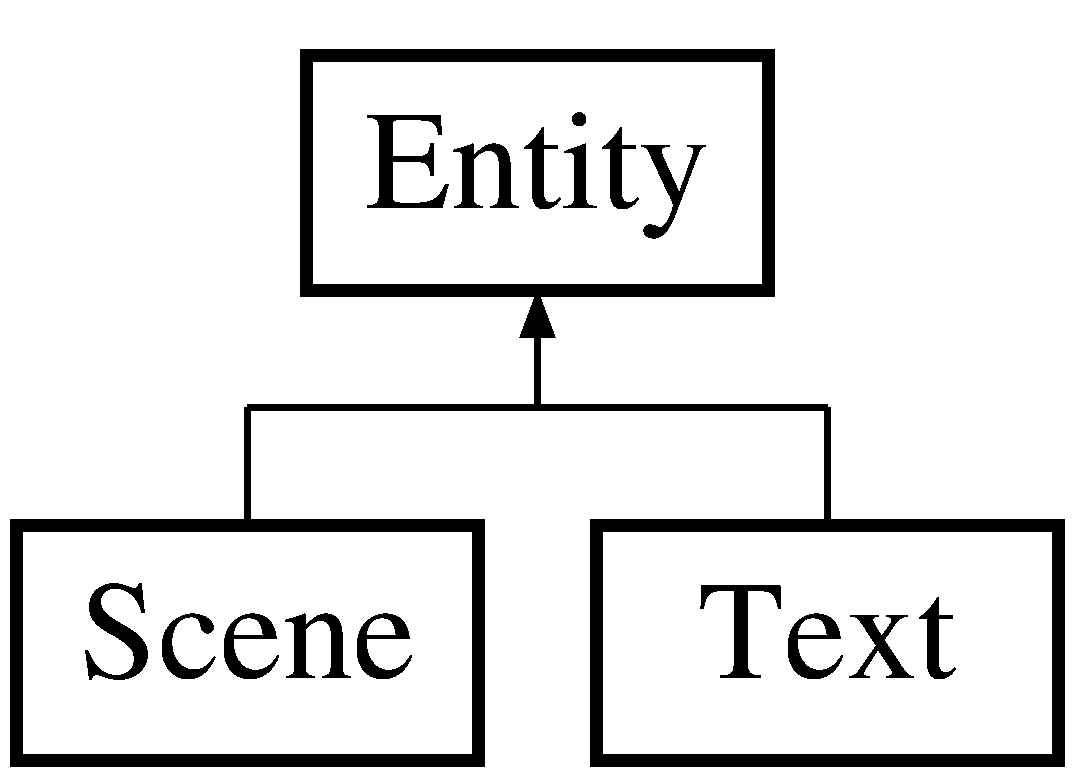
\includegraphics[height=2.000000cm]{class_entity}
\end{center}
\end{figure}
\subsection*{Public Member Functions}
\begin{DoxyCompactItemize}
\item 
\mbox{\Hypertarget{class_entity_a980f368aa07ce358583982821533a54a}\label{class_entity_a980f368aa07ce358583982821533a54a}} 
\hyperlink{class_entity_a980f368aa07ce358583982821533a54a}{Entity} ()
\begin{DoxyCompactList}\small\item\em Constructor of an \hyperlink{class_entity}{Entity}. \end{DoxyCompactList}\item 
\mbox{\Hypertarget{class_entity_adf6d3f7cb1b2ba029b6b048a395cc8ae}\label{class_entity_adf6d3f7cb1b2ba029b6b048a395cc8ae}} 
virtual \hyperlink{class_entity_adf6d3f7cb1b2ba029b6b048a395cc8ae}{$\sim$\+Entity} ()
\begin{DoxyCompactList}\small\item\em Destructor of an \hyperlink{class_entity}{Entity}. \end{DoxyCompactList}\item 
virtual void \hyperlink{class_entity_a7082aeb577c91707cc28edce571320f7}{update} (float delta\+Time)=0
\begin{DoxyCompactList}\small\item\em update this \hyperlink{class_entity}{Entity}. This function is Pure virtual. User M\+U\+ST implement this in subclass. \end{DoxyCompactList}\item 
void \hyperlink{class_entity_a445e5c82020eae36a145a692ff8482bc}{add\+Child} (\hyperlink{class_entity}{Entity} $\ast$child)
\begin{DoxyCompactList}\small\item\em add an \hyperlink{class_entity}{Entity} as a child of this \hyperlink{class_entity}{Entity}. Defines the data structure (parent/children relationship) \end{DoxyCompactList}\item 
void \hyperlink{class_entity_a45d5a3b92478ad8b4fb305b9b3e08c7a}{remove\+Child} (\hyperlink{class_entity}{Entity} $\ast$child)
\begin{DoxyCompactList}\small\item\em remove this \hyperlink{class_entity}{Entity} from list of children. \end{DoxyCompactList}\item 
\hyperlink{class_entity}{Entity} $\ast$ \hyperlink{class_entity_a86a7a735f9046c4ff3800a80f8ffd1ac}{get\+Child} (unsigned int i)
\begin{DoxyCompactList}\small\item\em get nth \hyperlink{class_entity}{Entity} from list of children. \end{DoxyCompactList}\item 
const std\+::vector$<$ \hyperlink{class_entity}{Entity} $\ast$ $>$ \& \hyperlink{class_entity_a1975d28f88ddd1afb83332245b194c79}{children} ()
\begin{DoxyCompactList}\small\item\em get the list of children. \end{DoxyCompactList}\item 
\hyperlink{class_sprite}{Sprite} $\ast$ \hyperlink{class_entity_a766b6c5da328efaa419bebe4f67479b9}{sprite} ()
\begin{DoxyCompactList}\small\item\em get the \hyperlink{class_sprite}{Sprite} from this \hyperlink{class_entity}{Entity}. \end{DoxyCompactList}\item 
void \hyperlink{class_entity_ae35b690cfec7ef9a0061338d7b83cfc4}{add\+Sprite} (\hyperlink{class_sprite}{Sprite} $\ast$spr)
\begin{DoxyCompactList}\small\item\em add a \hyperlink{class_sprite}{Sprite} to this \hyperlink{class_entity}{Entity} by Sprite$\ast$. \end{DoxyCompactList}\item 
void \hyperlink{class_entity_ab2501f9df0591cc5fd0535b15b2bb818}{add\+Sprite} (const std\+::string \&filename)
\begin{DoxyCompactList}\small\item\em add a \hyperlink{class_sprite}{Sprite} to this \hyperlink{class_entity}{Entity} by filename. \end{DoxyCompactList}\item 
void \hyperlink{class_entity_a5017dd79d0edad03fb7bd90df7eea867}{add\+Sprite} (const std\+::string \&filename, float pivotx, float pivoty)
\begin{DoxyCompactList}\small\item\em add a \hyperlink{class_sprite}{Sprite} to this \hyperlink{class_entity}{Entity}. \end{DoxyCompactList}\item 
void \hyperlink{class_entity_ae1a2eddd848404c8a9254f11036d00f5}{add\+Sprite} (const std\+::string \&filename, float pivotx, float pivoty, int filter, int wrap)
\begin{DoxyCompactList}\small\item\em add a \hyperlink{class_sprite}{Sprite} to this \hyperlink{class_entity}{Entity}. \end{DoxyCompactList}\item 
void \hyperlink{class_entity_a733aebaa5220f6dbd9b147aa8a9f6a3c}{add\+Sprite\+Sheet} (const std\+::string \&filename, int u, int v)
\begin{DoxyCompactList}\small\item\em add a Sprite\+Sheet to this \hyperlink{class_entity}{Entity}. \end{DoxyCompactList}\item 
void \hyperlink{class_entity_a3974e092fbb0f5984bf6806f83b62e33}{add\+Grid} (const std\+::string \&filename, int u, int v, int cols, int rows, int sizex, int sizey)
\begin{DoxyCompactList}\small\item\em add a Grid as a Spritebatch to this \hyperlink{class_entity}{Entity}. \end{DoxyCompactList}\item 
void \hyperlink{class_entity_a5a45a17006bcba507ffeeb33ddd6269e}{add\+Circle\+Sprite} (const std\+::string \&filename, int radius, int segments)
\begin{DoxyCompactList}\small\item\em add a Circular \hyperlink{class_sprite}{Sprite} to this \hyperlink{class_entity}{Entity} by filename. \end{DoxyCompactList}\item 
void \hyperlink{class_entity_a30b6c9e7d43616a622efa168b0b143e1}{add\+Segment\+Sprite} (const std\+::string \&filename, int radius, int segments, int which)
\begin{DoxyCompactList}\small\item\em add a Circular \hyperlink{class_sprite}{Sprite} to this \hyperlink{class_entity}{Entity} by filename. \end{DoxyCompactList}\item 
void \hyperlink{class_entity_adefc8fe3904ba419ac580c6aab09d770}{add\+Dynamic\+Sprite} (\hyperlink{struct_pixel_buffer}{Pixel\+Buffer} $\ast$pixels)
\begin{DoxyCompactList}\small\item\em add Dynamic \hyperlink{class_sprite}{Sprite} to this \hyperlink{class_entity}{Entity} by Pixel\+Buffer$\ast$. \end{DoxyCompactList}\item 
\hyperlink{class_line}{Line} $\ast$ \hyperlink{class_entity_a81cacd62804c930558bc2ff3f0c927ae}{line} ()
\begin{DoxyCompactList}\small\item\em get the \hyperlink{class_line}{Line} from this \hyperlink{class_entity}{Entity}. \end{DoxyCompactList}\item 
void \hyperlink{class_entity_a9acaf95e1437e0d8c068e3468846fefa}{add\+Line} (\hyperlink{class_line}{Line} $\ast$\hyperlink{class_entity_a81cacd62804c930558bc2ff3f0c927ae}{line})
\begin{DoxyCompactList}\small\item\em add a \hyperlink{class_line}{Line} to this \hyperlink{class_entity}{Entity} by Line$\ast$. \end{DoxyCompactList}\item 
void \hyperlink{class_entity_a9383f0d8ce804b216fc6e8164b4466a5}{add\+Line} (const std\+::string \&filename)
\begin{DoxyCompactList}\small\item\em add a \hyperlink{class_line}{Line} to this \hyperlink{class_entity}{Entity}. \end{DoxyCompactList}\item 
std\+::vector$<$ \hyperlink{class_sprite}{Sprite} $\ast$ $>$ \& \hyperlink{class_entity_a103d3fc8fff63075df60502c1966a7bc}{spritebatch} ()
\begin{DoxyCompactList}\small\item\em get the spritebatch of this \hyperlink{class_entity}{Entity}. \end{DoxyCompactList}\item 
int \hyperlink{class_entity_ad4f911b665f003d191c2940d325da6d8}{guid} ()
\begin{DoxyCompactList}\small\item\em get the guid of this \hyperlink{class_entity}{Entity}. \end{DoxyCompactList}\item 
\hyperlink{class_entity}{Entity} $\ast$ \hyperlink{class_entity_a9e2f02efca39cd7c4eca36e662372c25}{parent} ()
\begin{DoxyCompactList}\small\item\em get the parent of this \hyperlink{class_entity}{Entity}. \end{DoxyCompactList}\item 
\hyperlink{pointx_8h_aca903a92c8ced8823fea9fac7e23677a}{Point2} \hyperlink{class_entity_a85ae0243e89910d56dd7140c8f735f41}{worldpos} ()
\begin{DoxyCompactList}\small\item\em get the world position of this \hyperlink{class_entity}{Entity}. \end{DoxyCompactList}\end{DoxyCompactItemize}
\subsection*{Public Attributes}
\begin{DoxyCompactItemize}
\item 
\mbox{\Hypertarget{class_entity_af423990bd8393e6cbec1acf1c0b397ce}\label{class_entity_af423990bd8393e6cbec1acf1c0b397ce}} 
\hyperlink{pointx_8h_aca903a92c8ced8823fea9fac7e23677a}{Point2} \hyperlink{class_entity_af423990bd8393e6cbec1acf1c0b397ce}{position}
\begin{DoxyCompactList}\small\item\em The position of the \hyperlink{class_entity}{Entity}. \end{DoxyCompactList}\item 
\mbox{\Hypertarget{class_entity_aa384ccfdaba36b1ff5f5db51ec3cdcb1}\label{class_entity_aa384ccfdaba36b1ff5f5db51ec3cdcb1}} 
float \hyperlink{class_entity_aa384ccfdaba36b1ff5f5db51ec3cdcb1}{rotation}
\begin{DoxyCompactList}\small\item\em The rotation of the \hyperlink{class_entity}{Entity}. \end{DoxyCompactList}\item 
\mbox{\Hypertarget{class_entity_a286b63dabacf915914be06dfd37c0219}\label{class_entity_a286b63dabacf915914be06dfd37c0219}} 
\hyperlink{pointx_8h_aca903a92c8ced8823fea9fac7e23677a}{Point2} \hyperlink{class_entity_a286b63dabacf915914be06dfd37c0219}{scale}
\begin{DoxyCompactList}\small\item\em The scale of the \hyperlink{class_entity}{Entity}. \end{DoxyCompactList}\end{DoxyCompactItemize}
\subsection*{Protected Attributes}
\begin{DoxyCompactItemize}
\item 
\mbox{\Hypertarget{class_entity_aa8297d9903ba65954f51e400da52c3a9}\label{class_entity_aa8297d9903ba65954f51e400da52c3a9}} 
\hyperlink{pointx_8h_aca903a92c8ced8823fea9fac7e23677a}{Point2} \hyperlink{class_entity_aa8297d9903ba65954f51e400da52c3a9}{\+\_\+worldpos}
\begin{DoxyCompactList}\small\item\em The position of the \hyperlink{class_entity}{Entity} in the real world. \end{DoxyCompactList}\item 
\mbox{\Hypertarget{class_entity_a3927fd7358c34de5e2783bdf912cb9ed}\label{class_entity_a3927fd7358c34de5e2783bdf912cb9ed}} 
std\+::vector$<$ \hyperlink{class_sprite}{Sprite} $\ast$ $>$ \hyperlink{class_entity_a3927fd7358c34de5e2783bdf912cb9ed}{\+\_\+spritebatch}
\begin{DoxyCompactList}\small\item\em The \+\_\+spritebatch of this \hyperlink{class_entity}{Entity}. \end{DoxyCompactList}\end{DoxyCompactItemize}
\subsection*{Friends}
\begin{DoxyCompactItemize}
\item 
\mbox{\Hypertarget{class_entity_a70538530bc36e033e360880ef311df61}\label{class_entity_a70538530bc36e033e360880ef311df61}} 
class {\bfseries Renderer}
\end{DoxyCompactItemize}


\subsection{Detailed Description}
The \hyperlink{class_entity}{Entity} class is the Base class for the elements in your \hyperlink{class_scene}{Scene}. 

\subsection{Member Function Documentation}
\mbox{\Hypertarget{class_entity_a445e5c82020eae36a145a692ff8482bc}\label{class_entity_a445e5c82020eae36a145a692ff8482bc}} 
\index{Entity@{Entity}!add\+Child@{add\+Child}}
\index{add\+Child@{add\+Child}!Entity@{Entity}}
\subsubsection{\texorpdfstring{add\+Child()}{addChild()}}
{\footnotesize\ttfamily void Entity\+::add\+Child (\begin{DoxyParamCaption}\item[{\hyperlink{class_entity}{Entity} $\ast$}]{child }\end{DoxyParamCaption})}



add an \hyperlink{class_entity}{Entity} as a child of this \hyperlink{class_entity}{Entity}. Defines the data structure (parent/children relationship) 


\begin{DoxyParams}{Parameters}
{\em child} & The \hyperlink{class_entity}{Entity} you want to add as a child. \\
\hline
\end{DoxyParams}
\begin{DoxyReturn}{Returns}
void 
\end{DoxyReturn}
\mbox{\Hypertarget{class_entity_a5a45a17006bcba507ffeeb33ddd6269e}\label{class_entity_a5a45a17006bcba507ffeeb33ddd6269e}} 
\index{Entity@{Entity}!add\+Circle\+Sprite@{add\+Circle\+Sprite}}
\index{add\+Circle\+Sprite@{add\+Circle\+Sprite}!Entity@{Entity}}
\subsubsection{\texorpdfstring{add\+Circle\+Sprite()}{addCircleSprite()}}
{\footnotesize\ttfamily void Entity\+::add\+Circle\+Sprite (\begin{DoxyParamCaption}\item[{const std\+::string \&}]{filename,  }\item[{int}]{radius,  }\item[{int}]{segments }\end{DoxyParamCaption})}



add a Circular \hyperlink{class_sprite}{Sprite} to this \hyperlink{class_entity}{Entity} by filename. 


\begin{DoxyParams}{Parameters}
{\em filename} & The filename of the image you want to add as a \hyperlink{class_sprite}{Sprite}. \\
\hline
{\em radius} & The radius of the circle. \\
\hline
{\em segments} & The number of segments of the circle. \\
\hline
\end{DoxyParams}
\begin{DoxyReturn}{Returns}
void 
\end{DoxyReturn}
\mbox{\Hypertarget{class_entity_adefc8fe3904ba419ac580c6aab09d770}\label{class_entity_adefc8fe3904ba419ac580c6aab09d770}} 
\index{Entity@{Entity}!add\+Dynamic\+Sprite@{add\+Dynamic\+Sprite}}
\index{add\+Dynamic\+Sprite@{add\+Dynamic\+Sprite}!Entity@{Entity}}
\subsubsection{\texorpdfstring{add\+Dynamic\+Sprite()}{addDynamicSprite()}}
{\footnotesize\ttfamily void Entity\+::add\+Dynamic\+Sprite (\begin{DoxyParamCaption}\item[{\hyperlink{struct_pixel_buffer}{Pixel\+Buffer} $\ast$}]{pixels }\end{DoxyParamCaption})}



add Dynamic \hyperlink{class_sprite}{Sprite} to this \hyperlink{class_entity}{Entity} by Pixel\+Buffer$\ast$. 


\begin{DoxyParams}{Parameters}
{\em pixels} & A pointer to a \hyperlink{struct_pixel_buffer}{Pixel\+Buffer}. \\
\hline
\end{DoxyParams}
\begin{DoxyReturn}{Returns}
void 
\end{DoxyReturn}
\mbox{\Hypertarget{class_entity_a3974e092fbb0f5984bf6806f83b62e33}\label{class_entity_a3974e092fbb0f5984bf6806f83b62e33}} 
\index{Entity@{Entity}!add\+Grid@{add\+Grid}}
\index{add\+Grid@{add\+Grid}!Entity@{Entity}}
\subsubsection{\texorpdfstring{add\+Grid()}{addGrid()}}
{\footnotesize\ttfamily void Entity\+::add\+Grid (\begin{DoxyParamCaption}\item[{const std\+::string \&}]{filename,  }\item[{int}]{u,  }\item[{int}]{v,  }\item[{int}]{cols,  }\item[{int}]{rows,  }\item[{int}]{sizex,  }\item[{int}]{sizey }\end{DoxyParamCaption})}



add a Grid as a Spritebatch to this \hyperlink{class_entity}{Entity}. 


\begin{DoxyParams}{Parameters}
{\em filename} & The filename of the image. \\
\hline
{\em u} & number of horizontal textures \\
\hline
{\em v} & number of vertical textures \\
\hline
{\em cols} & number of cells \\
\hline
{\em rows} & number of vertical cells \\
\hline
{\em sizex} & horizontal size of a cell \\
\hline
{\em sizey} & vertical size of a cell \\
\hline
\end{DoxyParams}
\begin{DoxyReturn}{Returns}
void 
\end{DoxyReturn}
\mbox{\Hypertarget{class_entity_a9acaf95e1437e0d8c068e3468846fefa}\label{class_entity_a9acaf95e1437e0d8c068e3468846fefa}} 
\index{Entity@{Entity}!add\+Line@{add\+Line}}
\index{add\+Line@{add\+Line}!Entity@{Entity}}
\subsubsection{\texorpdfstring{add\+Line()}{addLine()}\hspace{0.1cm}{\footnotesize\ttfamily [1/2]}}
{\footnotesize\ttfamily void Entity\+::add\+Line (\begin{DoxyParamCaption}\item[{\hyperlink{class_line}{Line} $\ast$}]{line }\end{DoxyParamCaption})}



add a \hyperlink{class_line}{Line} to this \hyperlink{class_entity}{Entity} by Line$\ast$. 


\begin{DoxyParams}{Parameters}
{\em line} & A pointer to a \hyperlink{class_line}{Line}. \\
\hline
\end{DoxyParams}
\begin{DoxyReturn}{Returns}
void 
\end{DoxyReturn}
\mbox{\Hypertarget{class_entity_a9383f0d8ce804b216fc6e8164b4466a5}\label{class_entity_a9383f0d8ce804b216fc6e8164b4466a5}} 
\index{Entity@{Entity}!add\+Line@{add\+Line}}
\index{add\+Line@{add\+Line}!Entity@{Entity}}
\subsubsection{\texorpdfstring{add\+Line()}{addLine()}\hspace{0.1cm}{\footnotesize\ttfamily [2/2]}}
{\footnotesize\ttfamily void Entity\+::add\+Line (\begin{DoxyParamCaption}\item[{const std\+::string \&}]{filename }\end{DoxyParamCaption})}



add a \hyperlink{class_line}{Line} to this \hyperlink{class_entity}{Entity}. 


\begin{DoxyParams}{Parameters}
{\em filename} & The filename of the line you want to add. \\
\hline
\end{DoxyParams}
\begin{DoxyReturn}{Returns}
void 
\end{DoxyReturn}
\mbox{\Hypertarget{class_entity_a30b6c9e7d43616a622efa168b0b143e1}\label{class_entity_a30b6c9e7d43616a622efa168b0b143e1}} 
\index{Entity@{Entity}!add\+Segment\+Sprite@{add\+Segment\+Sprite}}
\index{add\+Segment\+Sprite@{add\+Segment\+Sprite}!Entity@{Entity}}
\subsubsection{\texorpdfstring{add\+Segment\+Sprite()}{addSegmentSprite()}}
{\footnotesize\ttfamily void Entity\+::add\+Segment\+Sprite (\begin{DoxyParamCaption}\item[{const std\+::string \&}]{filename,  }\item[{int}]{radius,  }\item[{int}]{segments,  }\item[{int}]{which }\end{DoxyParamCaption})}



add a Circular \hyperlink{class_sprite}{Sprite} to this \hyperlink{class_entity}{Entity} by filename. 


\begin{DoxyParams}{Parameters}
{\em filename} & The filename of the image you want to add as a \hyperlink{class_sprite}{Sprite}. \\
\hline
{\em radius} & The radius of the circle. \\
\hline
{\em segments} & The number of segments of the circle. \\
\hline
{\em which} & which segment (0-\/5 if hexagon). \\
\hline
\end{DoxyParams}
\begin{DoxyReturn}{Returns}
void 
\end{DoxyReturn}
\mbox{\Hypertarget{class_entity_ae35b690cfec7ef9a0061338d7b83cfc4}\label{class_entity_ae35b690cfec7ef9a0061338d7b83cfc4}} 
\index{Entity@{Entity}!add\+Sprite@{add\+Sprite}}
\index{add\+Sprite@{add\+Sprite}!Entity@{Entity}}
\subsubsection{\texorpdfstring{add\+Sprite()}{addSprite()}\hspace{0.1cm}{\footnotesize\ttfamily [1/4]}}
{\footnotesize\ttfamily void Entity\+::add\+Sprite (\begin{DoxyParamCaption}\item[{\hyperlink{class_sprite}{Sprite} $\ast$}]{spr }\end{DoxyParamCaption})}



add a \hyperlink{class_sprite}{Sprite} to this \hyperlink{class_entity}{Entity} by Sprite$\ast$. 


\begin{DoxyParams}{Parameters}
{\em spr} & A pointer to a \hyperlink{class_sprite}{Sprite}. \\
\hline
\end{DoxyParams}
\begin{DoxyReturn}{Returns}
void 
\end{DoxyReturn}
\mbox{\Hypertarget{class_entity_ab2501f9df0591cc5fd0535b15b2bb818}\label{class_entity_ab2501f9df0591cc5fd0535b15b2bb818}} 
\index{Entity@{Entity}!add\+Sprite@{add\+Sprite}}
\index{add\+Sprite@{add\+Sprite}!Entity@{Entity}}
\subsubsection{\texorpdfstring{add\+Sprite()}{addSprite()}\hspace{0.1cm}{\footnotesize\ttfamily [2/4]}}
{\footnotesize\ttfamily void Entity\+::add\+Sprite (\begin{DoxyParamCaption}\item[{const std\+::string \&}]{filename }\end{DoxyParamCaption})}



add a \hyperlink{class_sprite}{Sprite} to this \hyperlink{class_entity}{Entity} by filename. 


\begin{DoxyParams}{Parameters}
{\em filename} & The filename of the image you want to add as a \hyperlink{class_sprite}{Sprite}. \\
\hline
\end{DoxyParams}
\begin{DoxyReturn}{Returns}
void 
\end{DoxyReturn}
\mbox{\Hypertarget{class_entity_a5017dd79d0edad03fb7bd90df7eea867}\label{class_entity_a5017dd79d0edad03fb7bd90df7eea867}} 
\index{Entity@{Entity}!add\+Sprite@{add\+Sprite}}
\index{add\+Sprite@{add\+Sprite}!Entity@{Entity}}
\subsubsection{\texorpdfstring{add\+Sprite()}{addSprite()}\hspace{0.1cm}{\footnotesize\ttfamily [3/4]}}
{\footnotesize\ttfamily void Entity\+::add\+Sprite (\begin{DoxyParamCaption}\item[{const std\+::string \&}]{filename,  }\item[{float}]{pivotx,  }\item[{float}]{pivoty }\end{DoxyParamCaption})}



add a \hyperlink{class_sprite}{Sprite} to this \hyperlink{class_entity}{Entity}. 


\begin{DoxyParams}{Parameters}
{\em filename} & The filename of the image you want to add as a \hyperlink{class_sprite}{Sprite}. \\
\hline
{\em pivotx} & The x component of the pivotpoint. \\
\hline
{\em pivoty} & The y component of the pivotpoint. \\
\hline
\end{DoxyParams}
\begin{DoxyReturn}{Returns}
void 
\end{DoxyReturn}
\mbox{\Hypertarget{class_entity_ae1a2eddd848404c8a9254f11036d00f5}\label{class_entity_ae1a2eddd848404c8a9254f11036d00f5}} 
\index{Entity@{Entity}!add\+Sprite@{add\+Sprite}}
\index{add\+Sprite@{add\+Sprite}!Entity@{Entity}}
\subsubsection{\texorpdfstring{add\+Sprite()}{addSprite()}\hspace{0.1cm}{\footnotesize\ttfamily [4/4]}}
{\footnotesize\ttfamily void Entity\+::add\+Sprite (\begin{DoxyParamCaption}\item[{const std\+::string \&}]{filename,  }\item[{float}]{pivotx,  }\item[{float}]{pivoty,  }\item[{int}]{filter,  }\item[{int}]{wrap }\end{DoxyParamCaption})}



add a \hyperlink{class_sprite}{Sprite} to this \hyperlink{class_entity}{Entity}. 


\begin{DoxyParams}{Parameters}
{\em filename} & The filename of the image you want to add as a \hyperlink{class_sprite}{Sprite}. \\
\hline
{\em pivotx} & The x component of the pivotpoint. \\
\hline
{\em pivoty} & The y component of the pivotpoint. \\
\hline
{\em filter} & The filter. \\
\hline
{\em wrap} & The wrapping. \\
\hline
\end{DoxyParams}
\begin{DoxyReturn}{Returns}
void 
\end{DoxyReturn}
\mbox{\Hypertarget{class_entity_a733aebaa5220f6dbd9b147aa8a9f6a3c}\label{class_entity_a733aebaa5220f6dbd9b147aa8a9f6a3c}} 
\index{Entity@{Entity}!add\+Sprite\+Sheet@{add\+Sprite\+Sheet}}
\index{add\+Sprite\+Sheet@{add\+Sprite\+Sheet}!Entity@{Entity}}
\subsubsection{\texorpdfstring{add\+Sprite\+Sheet()}{addSpriteSheet()}}
{\footnotesize\ttfamily void Entity\+::add\+Sprite\+Sheet (\begin{DoxyParamCaption}\item[{const std\+::string \&}]{filename,  }\item[{int}]{u,  }\item[{int}]{v }\end{DoxyParamCaption})}



add a Sprite\+Sheet to this \hyperlink{class_entity}{Entity}. 


\begin{DoxyParams}{Parameters}
{\em filename} & The filename of the image you want to add as a Sprite\+Sheet. \\
\hline
{\em u} & number of horizontal textures \\
\hline
{\em v} & number of vertical textures \\
\hline
\end{DoxyParams}
\begin{DoxyReturn}{Returns}
void 
\end{DoxyReturn}
\mbox{\Hypertarget{class_entity_a1975d28f88ddd1afb83332245b194c79}\label{class_entity_a1975d28f88ddd1afb83332245b194c79}} 
\index{Entity@{Entity}!children@{children}}
\index{children@{children}!Entity@{Entity}}
\subsubsection{\texorpdfstring{children()}{children()}}
{\footnotesize\ttfamily const std\+::vector$<$\hyperlink{class_entity}{Entity}$\ast$$>$\& Entity\+::children (\begin{DoxyParamCaption}{ }\end{DoxyParamCaption})\hspace{0.3cm}{\ttfamily [inline]}}



get the list of children. 

\begin{DoxyReturn}{Returns}
std\+::vector$<$\+Entity$\ast$$>$\& \+\_\+children 
\end{DoxyReturn}
\mbox{\Hypertarget{class_entity_a86a7a735f9046c4ff3800a80f8ffd1ac}\label{class_entity_a86a7a735f9046c4ff3800a80f8ffd1ac}} 
\index{Entity@{Entity}!get\+Child@{get\+Child}}
\index{get\+Child@{get\+Child}!Entity@{Entity}}
\subsubsection{\texorpdfstring{get\+Child()}{getChild()}}
{\footnotesize\ttfamily \hyperlink{class_entity}{Entity} $\ast$ Entity\+::get\+Child (\begin{DoxyParamCaption}\item[{unsigned int}]{i }\end{DoxyParamCaption})}



get nth \hyperlink{class_entity}{Entity} from list of children. 


\begin{DoxyParams}{Parameters}
{\em i} & The id of the \hyperlink{class_entity}{Entity} you want to get. \\
\hline
\end{DoxyParams}
\begin{DoxyReturn}{Returns}
Entity$\ast$ child 
\end{DoxyReturn}
\mbox{\Hypertarget{class_entity_ad4f911b665f003d191c2940d325da6d8}\label{class_entity_ad4f911b665f003d191c2940d325da6d8}} 
\index{Entity@{Entity}!guid@{guid}}
\index{guid@{guid}!Entity@{Entity}}
\subsubsection{\texorpdfstring{guid()}{guid()}}
{\footnotesize\ttfamily int Entity\+::guid (\begin{DoxyParamCaption}{ }\end{DoxyParamCaption})\hspace{0.3cm}{\ttfamily [inline]}}



get the guid of this \hyperlink{class_entity}{Entity}. 

\begin{DoxyReturn}{Returns}
int \+\_\+guid 
\end{DoxyReturn}
\mbox{\Hypertarget{class_entity_a81cacd62804c930558bc2ff3f0c927ae}\label{class_entity_a81cacd62804c930558bc2ff3f0c927ae}} 
\index{Entity@{Entity}!line@{line}}
\index{line@{line}!Entity@{Entity}}
\subsubsection{\texorpdfstring{line()}{line()}}
{\footnotesize\ttfamily \hyperlink{class_line}{Line}$\ast$ Entity\+::line (\begin{DoxyParamCaption}{ }\end{DoxyParamCaption})\hspace{0.3cm}{\ttfamily [inline]}}



get the \hyperlink{class_line}{Line} from this \hyperlink{class_entity}{Entity}. 

\begin{DoxyReturn}{Returns}
Line$\ast$ \+\_\+line 
\end{DoxyReturn}
\mbox{\Hypertarget{class_entity_a9e2f02efca39cd7c4eca36e662372c25}\label{class_entity_a9e2f02efca39cd7c4eca36e662372c25}} 
\index{Entity@{Entity}!parent@{parent}}
\index{parent@{parent}!Entity@{Entity}}
\subsubsection{\texorpdfstring{parent()}{parent()}}
{\footnotesize\ttfamily \hyperlink{class_entity}{Entity}$\ast$ Entity\+::parent (\begin{DoxyParamCaption}{ }\end{DoxyParamCaption})\hspace{0.3cm}{\ttfamily [inline]}}



get the parent of this \hyperlink{class_entity}{Entity}. 

\begin{DoxyReturn}{Returns}
Entity$\ast$ \+\_\+parent 
\end{DoxyReturn}
\mbox{\Hypertarget{class_entity_a45d5a3b92478ad8b4fb305b9b3e08c7a}\label{class_entity_a45d5a3b92478ad8b4fb305b9b3e08c7a}} 
\index{Entity@{Entity}!remove\+Child@{remove\+Child}}
\index{remove\+Child@{remove\+Child}!Entity@{Entity}}
\subsubsection{\texorpdfstring{remove\+Child()}{removeChild()}}
{\footnotesize\ttfamily void Entity\+::remove\+Child (\begin{DoxyParamCaption}\item[{\hyperlink{class_entity}{Entity} $\ast$}]{child }\end{DoxyParamCaption})}



remove this \hyperlink{class_entity}{Entity} from list of children. 


\begin{DoxyParams}{Parameters}
{\em child} & The \hyperlink{class_entity}{Entity} you want to remove from your children. \\
\hline
\end{DoxyParams}
\begin{DoxyReturn}{Returns}
void 
\end{DoxyReturn}
\mbox{\Hypertarget{class_entity_a766b6c5da328efaa419bebe4f67479b9}\label{class_entity_a766b6c5da328efaa419bebe4f67479b9}} 
\index{Entity@{Entity}!sprite@{sprite}}
\index{sprite@{sprite}!Entity@{Entity}}
\subsubsection{\texorpdfstring{sprite()}{sprite()}}
{\footnotesize\ttfamily \hyperlink{class_sprite}{Sprite}$\ast$ Entity\+::sprite (\begin{DoxyParamCaption}{ }\end{DoxyParamCaption})\hspace{0.3cm}{\ttfamily [inline]}}



get the \hyperlink{class_sprite}{Sprite} from this \hyperlink{class_entity}{Entity}. 

\begin{DoxyReturn}{Returns}
Sprite$\ast$ \+\_\+sprite 
\end{DoxyReturn}
\mbox{\Hypertarget{class_entity_a103d3fc8fff63075df60502c1966a7bc}\label{class_entity_a103d3fc8fff63075df60502c1966a7bc}} 
\index{Entity@{Entity}!spritebatch@{spritebatch}}
\index{spritebatch@{spritebatch}!Entity@{Entity}}
\subsubsection{\texorpdfstring{spritebatch()}{spritebatch()}}
{\footnotesize\ttfamily std\+::vector$<$\hyperlink{class_sprite}{Sprite}$\ast$$>$\& Entity\+::spritebatch (\begin{DoxyParamCaption}{ }\end{DoxyParamCaption})\hspace{0.3cm}{\ttfamily [inline]}}



get the spritebatch of this \hyperlink{class_entity}{Entity}. 

\begin{DoxyReturn}{Returns}
std\+::vector$<$\+Sprite$\ast$$>$\& \+\_\+spritebatch 
\end{DoxyReturn}
\mbox{\Hypertarget{class_entity_a7082aeb577c91707cc28edce571320f7}\label{class_entity_a7082aeb577c91707cc28edce571320f7}} 
\index{Entity@{Entity}!update@{update}}
\index{update@{update}!Entity@{Entity}}
\subsubsection{\texorpdfstring{update()}{update()}}
{\footnotesize\ttfamily virtual void Entity\+::update (\begin{DoxyParamCaption}\item[{float}]{delta\+Time }\end{DoxyParamCaption})\hspace{0.3cm}{\ttfamily [pure virtual]}}



update this \hyperlink{class_entity}{Entity}. This function is Pure virtual. User M\+U\+ST implement this in subclass. 


\begin{DoxyParams}{Parameters}
{\em delta\+Time} & The time that\textquotesingle{}s passed since the last update. \\
\hline
\end{DoxyParams}
\begin{DoxyReturn}{Returns}
void 
\end{DoxyReturn}


Implemented in \hyperlink{class_text_a5604f1f74fd487d2972d024575497484}{Text}.

\mbox{\Hypertarget{class_entity_a85ae0243e89910d56dd7140c8f735f41}\label{class_entity_a85ae0243e89910d56dd7140c8f735f41}} 
\index{Entity@{Entity}!worldpos@{worldpos}}
\index{worldpos@{worldpos}!Entity@{Entity}}
\subsubsection{\texorpdfstring{worldpos()}{worldpos()}}
{\footnotesize\ttfamily \hyperlink{pointx_8h_aca903a92c8ced8823fea9fac7e23677a}{Point2} Entity\+::worldpos (\begin{DoxyParamCaption}{ }\end{DoxyParamCaption})\hspace{0.3cm}{\ttfamily [inline]}}



get the world position of this \hyperlink{class_entity}{Entity}. 

\begin{DoxyReturn}{Returns}
Point2 \+\_\+worldpos 
\end{DoxyReturn}


The documentation for this class was generated from the following files\+:\begin{DoxyCompactItemize}
\item 
\hyperlink{entity_8h}{entity.\+h}\item 
entity.\+cpp\end{DoxyCompactItemize}

\hypertarget{struct_h_s_v_color}{}\section{H\+S\+V\+Color Struct Reference}
\label{struct_h_s_v_color}\index{H\+S\+V\+Color@{H\+S\+V\+Color}}


A 24 bit H\+SV color.  




{\ttfamily \#include $<$color.\+h$>$}

\subsection*{Public Member Functions}
\begin{DoxyCompactItemize}
\item 
\mbox{\Hypertarget{struct_h_s_v_color_ab2cd8175fa87c007d9ae98d09ae39d9f}\label{struct_h_s_v_color_ab2cd8175fa87c007d9ae98d09ae39d9f}} 
\hyperlink{struct_h_s_v_color_ab2cd8175fa87c007d9ae98d09ae39d9f}{H\+S\+V\+Color} ()
\begin{DoxyCompactList}\small\item\em constructor \end{DoxyCompactList}\item 
\hyperlink{struct_h_s_v_color_a774e6af3f0c2fcf755c1cddaeac1c0d8}{H\+S\+V\+Color} (float hue, float sat, float val)
\begin{DoxyCompactList}\small\item\em constructor \end{DoxyCompactList}\end{DoxyCompactItemize}
\subsection*{Public Attributes}
\begin{DoxyCompactItemize}
\item 
\mbox{\Hypertarget{struct_h_s_v_color_a015d43b1226532d7748e4c0b77d8f5fa}\label{struct_h_s_v_color_a015d43b1226532d7748e4c0b77d8f5fa}} 
float \hyperlink{struct_h_s_v_color_a015d43b1226532d7748e4c0b77d8f5fa}{h} = 0.\+0f
\begin{DoxyCompactList}\small\item\em The Hue component of the color. \end{DoxyCompactList}\item 
\mbox{\Hypertarget{struct_h_s_v_color_a2935d350bd1966b6988a09a8867de625}\label{struct_h_s_v_color_a2935d350bd1966b6988a09a8867de625}} 
float \hyperlink{struct_h_s_v_color_a2935d350bd1966b6988a09a8867de625}{s} = 0.\+0f
\begin{DoxyCompactList}\small\item\em The Saturation component of the color. \end{DoxyCompactList}\item 
\mbox{\Hypertarget{struct_h_s_v_color_a03308eb73b5b24d31a994ae8f80768ee}\label{struct_h_s_v_color_a03308eb73b5b24d31a994ae8f80768ee}} 
float \hyperlink{struct_h_s_v_color_a03308eb73b5b24d31a994ae8f80768ee}{v} = 1.\+0f
\begin{DoxyCompactList}\small\item\em The Lightness/\+Brightness/\+Value component of the color. \end{DoxyCompactList}\end{DoxyCompactItemize}


\subsection{Detailed Description}
A 24 bit H\+SV color. 

A struct that defines an H\+SV \hyperlink{struct_color}{Color} (Hue, Saturation, Brightness). Each value is a float between 0.\+0f and 1.\+0f. 

\subsection{Constructor \& Destructor Documentation}
\mbox{\Hypertarget{struct_h_s_v_color_a774e6af3f0c2fcf755c1cddaeac1c0d8}\label{struct_h_s_v_color_a774e6af3f0c2fcf755c1cddaeac1c0d8}} 
\index{H\+S\+V\+Color@{H\+S\+V\+Color}!H\+S\+V\+Color@{H\+S\+V\+Color}}
\index{H\+S\+V\+Color@{H\+S\+V\+Color}!H\+S\+V\+Color@{H\+S\+V\+Color}}
\subsubsection{\texorpdfstring{H\+S\+V\+Color()}{HSVColor()}}
{\footnotesize\ttfamily H\+S\+V\+Color\+::\+H\+S\+V\+Color (\begin{DoxyParamCaption}\item[{float}]{hue,  }\item[{float}]{sat,  }\item[{float}]{val }\end{DoxyParamCaption})\hspace{0.3cm}{\ttfamily [inline]}}



constructor 


\begin{DoxyParams}{Parameters}
{\em hue} & The hue component of the color \\
\hline
{\em sat} & The saturation component of the color \\
\hline
{\em val} & The brightness/lightness/value component of the color \\
\hline
\end{DoxyParams}


The documentation for this struct was generated from the following file\+:\begin{DoxyCompactItemize}
\item 
\hyperlink{color_8h}{color.\+h}\end{DoxyCompactItemize}

\hypertarget{class_input}{}\section{Input Class Reference}
\label{class_input}\index{Input@{Input}}


The \hyperlink{class_input}{Input} class handles Keyboard and Mouse.  




{\ttfamily \#include $<$input.\+h$>$}

\subsection*{Public Member Functions}
\begin{DoxyCompactItemize}
\item 
\hyperlink{class_input_abae3f379d3f157cf42dc857309832dba}{Input} ()
\begin{DoxyCompactList}\small\item\em Constructor of the \hyperlink{class_input}{Input}. \end{DoxyCompactList}\item 
\mbox{\Hypertarget{class_input_af2db35ba67c8a8ccd23bef6a482fc291}\label{class_input_af2db35ba67c8a8ccd23bef6a482fc291}} 
virtual \hyperlink{class_input_af2db35ba67c8a8ccd23bef6a482fc291}{$\sim$\+Input} ()
\begin{DoxyCompactList}\small\item\em Destructor of the \hyperlink{class_input}{Input}. \end{DoxyCompactList}\item 
void \hyperlink{class_input_a6fcfdeb17f2db772a1058274a8fac43e}{update\+Input} (G\+L\+F\+Wwindow $\ast$w)
\begin{DoxyCompactList}\small\item\em updates the input from Keyboard and Mouse. \end{DoxyCompactList}\item 
bool \hyperlink{class_input_a62ca94f9d79e246423a8a6e46d6e88dc}{get\+Key} (int key)
\begin{DoxyCompactList}\small\item\em Is this key pressed? \end{DoxyCompactList}\item 
bool \hyperlink{class_input_a9759385ef5234448861d0330a205c40b}{get\+Key} (char key)
\begin{DoxyCompactList}\small\item\em Is this key pressed? \end{DoxyCompactList}\item 
bool \hyperlink{class_input_a3e7ca67c5c02f7e6516013c987339d05}{get\+Mouse} (int button)
\begin{DoxyCompactList}\small\item\em Is this mouse button pressed? \end{DoxyCompactList}\item 
bool \hyperlink{class_input_a96d176060e37d81a0f0c4fef52083b92}{get\+Key\+Down} (int key)
\begin{DoxyCompactList}\small\item\em Is this key pressed? Only check first press down. \end{DoxyCompactList}\item 
bool \hyperlink{class_input_a17110267d046bf4ec55f58b2e3f271f2}{get\+Key\+Down} (char key)
\begin{DoxyCompactList}\small\item\em Is this key pressed? Only check first press down. \end{DoxyCompactList}\item 
bool \hyperlink{class_input_aac8e9e5714c33bc9d3e478e2472fdc10}{get\+Mouse\+Down} (int button)
\begin{DoxyCompactList}\small\item\em Is this mouse button pressed? Only check first press down. \end{DoxyCompactList}\item 
bool \hyperlink{class_input_a965184281347f881d145aac555b727d7}{get\+Key\+Up} (int key)
\begin{DoxyCompactList}\small\item\em Is this key released? \end{DoxyCompactList}\item 
bool \hyperlink{class_input_a4e75aadc94c3d0fb2b236388b5dddec7}{get\+Key\+Up} (char key)
\begin{DoxyCompactList}\small\item\em Is this key released? \end{DoxyCompactList}\item 
bool \hyperlink{class_input_ad5c2b0983d6319b90ccbe1103f962736}{get\+Mouse\+Up} (int button)
\begin{DoxyCompactList}\small\item\em Is this mouse button released? \end{DoxyCompactList}\item 
double \hyperlink{class_input_a998ef567ed9101db034b8274b2543e1b}{get\+MouseX} ()
\begin{DoxyCompactList}\small\item\em get X position of the Mouse \end{DoxyCompactList}\item 
double \hyperlink{class_input_afdb964d8fffbbc6bab1d3b34648c1543}{get\+MouseY} ()
\begin{DoxyCompactList}\small\item\em get Y position of the Mouse \end{DoxyCompactList}\item 
void \hyperlink{class_input_a2c477753baedd21924670f0a16260160}{set\+Mouse} (double x, double y)
\begin{DoxyCompactList}\small\item\em Set Mouse cursor to a certain position. \end{DoxyCompactList}\item 
int \hyperlink{class_input_a8e4f99acfe8cadda2879697be26bf295}{get\+Window\+Width} ()
\begin{DoxyCompactList}\small\item\em get width of the window \end{DoxyCompactList}\item 
int \hyperlink{class_input_a3eccc8d5cd466b7ec312e3af7b801473}{get\+Window\+Height} ()
\begin{DoxyCompactList}\small\item\em get height of the window \end{DoxyCompactList}\end{DoxyCompactItemize}


\subsection{Detailed Description}
The \hyperlink{class_input}{Input} class handles Keyboard and Mouse. 

\subsection{Constructor \& Destructor Documentation}
\mbox{\Hypertarget{class_input_abae3f379d3f157cf42dc857309832dba}\label{class_input_abae3f379d3f157cf42dc857309832dba}} 
\index{Input@{Input}!Input@{Input}}
\index{Input@{Input}!Input@{Input}}
\subsubsection{\texorpdfstring{Input()}{Input()}}
{\footnotesize\ttfamily Input\+::\+Input (\begin{DoxyParamCaption}{ }\end{DoxyParamCaption})}



Constructor of the \hyperlink{class_input}{Input}. 

This file is part of R\+T2D, a 2D Open\+GL framework.


\begin{DoxyItemize}
\item Copyright 2015 Rik Teerling \href{mailto:rik@onandoffables.com}{\tt rik@onandoffables.\+com}
\begin{DoxyItemize}
\item Initial commit
\item \mbox{[}meruiden\mbox{]} scaling of window 
\end{DoxyItemize}
\end{DoxyItemize}

\subsection{Member Function Documentation}
\mbox{\Hypertarget{class_input_a62ca94f9d79e246423a8a6e46d6e88dc}\label{class_input_a62ca94f9d79e246423a8a6e46d6e88dc}} 
\index{Input@{Input}!get\+Key@{get\+Key}}
\index{get\+Key@{get\+Key}!Input@{Input}}
\subsubsection{\texorpdfstring{get\+Key()}{getKey()}\hspace{0.1cm}{\footnotesize\ttfamily [1/2]}}
{\footnotesize\ttfamily bool Input\+::get\+Key (\begin{DoxyParamCaption}\item[{int}]{key }\end{DoxyParamCaption})\hspace{0.3cm}{\ttfamily [inline]}}



Is this key pressed? 


\begin{DoxyParams}{Parameters}
{\em key} & as int (see defines) \\
\hline
\end{DoxyParams}
\begin{DoxyReturn}{Returns}
bool key is pressed or not 
\end{DoxyReturn}
\mbox{\Hypertarget{class_input_a9759385ef5234448861d0330a205c40b}\label{class_input_a9759385ef5234448861d0330a205c40b}} 
\index{Input@{Input}!get\+Key@{get\+Key}}
\index{get\+Key@{get\+Key}!Input@{Input}}
\subsubsection{\texorpdfstring{get\+Key()}{getKey()}\hspace{0.1cm}{\footnotesize\ttfamily [2/2]}}
{\footnotesize\ttfamily bool Input\+::get\+Key (\begin{DoxyParamCaption}\item[{char}]{key }\end{DoxyParamCaption})\hspace{0.3cm}{\ttfamily [inline]}}



Is this key pressed? 


\begin{DoxyParams}{Parameters}
{\em key} & as char (ie \textquotesingle{}a\textquotesingle{}) \\
\hline
\end{DoxyParams}
\begin{DoxyReturn}{Returns}
bool key is pressed or not 
\end{DoxyReturn}
\mbox{\Hypertarget{class_input_a96d176060e37d81a0f0c4fef52083b92}\label{class_input_a96d176060e37d81a0f0c4fef52083b92}} 
\index{Input@{Input}!get\+Key\+Down@{get\+Key\+Down}}
\index{get\+Key\+Down@{get\+Key\+Down}!Input@{Input}}
\subsubsection{\texorpdfstring{get\+Key\+Down()}{getKeyDown()}\hspace{0.1cm}{\footnotesize\ttfamily [1/2]}}
{\footnotesize\ttfamily bool Input\+::get\+Key\+Down (\begin{DoxyParamCaption}\item[{int}]{key }\end{DoxyParamCaption})\hspace{0.3cm}{\ttfamily [inline]}}



Is this key pressed? Only check first press down. 


\begin{DoxyParams}{Parameters}
{\em key} & as int (see defines) \\
\hline
\end{DoxyParams}
\begin{DoxyReturn}{Returns}
bool key is pressed first time or not 
\end{DoxyReturn}
\mbox{\Hypertarget{class_input_a17110267d046bf4ec55f58b2e3f271f2}\label{class_input_a17110267d046bf4ec55f58b2e3f271f2}} 
\index{Input@{Input}!get\+Key\+Down@{get\+Key\+Down}}
\index{get\+Key\+Down@{get\+Key\+Down}!Input@{Input}}
\subsubsection{\texorpdfstring{get\+Key\+Down()}{getKeyDown()}\hspace{0.1cm}{\footnotesize\ttfamily [2/2]}}
{\footnotesize\ttfamily bool Input\+::get\+Key\+Down (\begin{DoxyParamCaption}\item[{char}]{key }\end{DoxyParamCaption})\hspace{0.3cm}{\ttfamily [inline]}}



Is this key pressed? Only check first press down. 


\begin{DoxyParams}{Parameters}
{\em key} & as char (ie \textquotesingle{}a\textquotesingle{}) \\
\hline
\end{DoxyParams}
\begin{DoxyReturn}{Returns}
bool key is pressed first time or not 
\end{DoxyReturn}
\mbox{\Hypertarget{class_input_a965184281347f881d145aac555b727d7}\label{class_input_a965184281347f881d145aac555b727d7}} 
\index{Input@{Input}!get\+Key\+Up@{get\+Key\+Up}}
\index{get\+Key\+Up@{get\+Key\+Up}!Input@{Input}}
\subsubsection{\texorpdfstring{get\+Key\+Up()}{getKeyUp()}\hspace{0.1cm}{\footnotesize\ttfamily [1/2]}}
{\footnotesize\ttfamily bool Input\+::get\+Key\+Up (\begin{DoxyParamCaption}\item[{int}]{key }\end{DoxyParamCaption})\hspace{0.3cm}{\ttfamily [inline]}}



Is this key released? 


\begin{DoxyParams}{Parameters}
{\em key} & as int (see defines) \\
\hline
\end{DoxyParams}
\begin{DoxyReturn}{Returns}
bool true or false 
\end{DoxyReturn}
\mbox{\Hypertarget{class_input_a4e75aadc94c3d0fb2b236388b5dddec7}\label{class_input_a4e75aadc94c3d0fb2b236388b5dddec7}} 
\index{Input@{Input}!get\+Key\+Up@{get\+Key\+Up}}
\index{get\+Key\+Up@{get\+Key\+Up}!Input@{Input}}
\subsubsection{\texorpdfstring{get\+Key\+Up()}{getKeyUp()}\hspace{0.1cm}{\footnotesize\ttfamily [2/2]}}
{\footnotesize\ttfamily bool Input\+::get\+Key\+Up (\begin{DoxyParamCaption}\item[{char}]{key }\end{DoxyParamCaption})\hspace{0.3cm}{\ttfamily [inline]}}



Is this key released? 


\begin{DoxyParams}{Parameters}
{\em key} & as char (ie \textquotesingle{}a\textquotesingle{}) \\
\hline
\end{DoxyParams}
\begin{DoxyReturn}{Returns}
bool key is released or not 
\end{DoxyReturn}
\mbox{\Hypertarget{class_input_a3e7ca67c5c02f7e6516013c987339d05}\label{class_input_a3e7ca67c5c02f7e6516013c987339d05}} 
\index{Input@{Input}!get\+Mouse@{get\+Mouse}}
\index{get\+Mouse@{get\+Mouse}!Input@{Input}}
\subsubsection{\texorpdfstring{get\+Mouse()}{getMouse()}}
{\footnotesize\ttfamily bool Input\+::get\+Mouse (\begin{DoxyParamCaption}\item[{int}]{button }\end{DoxyParamCaption})\hspace{0.3cm}{\ttfamily [inline]}}



Is this mouse button pressed? 


\begin{DoxyParams}{Parameters}
{\em button} & num \\
\hline
\end{DoxyParams}
\begin{DoxyReturn}{Returns}
bool button is pressed or not 
\end{DoxyReturn}
\mbox{\Hypertarget{class_input_aac8e9e5714c33bc9d3e478e2472fdc10}\label{class_input_aac8e9e5714c33bc9d3e478e2472fdc10}} 
\index{Input@{Input}!get\+Mouse\+Down@{get\+Mouse\+Down}}
\index{get\+Mouse\+Down@{get\+Mouse\+Down}!Input@{Input}}
\subsubsection{\texorpdfstring{get\+Mouse\+Down()}{getMouseDown()}}
{\footnotesize\ttfamily bool Input\+::get\+Mouse\+Down (\begin{DoxyParamCaption}\item[{int}]{button }\end{DoxyParamCaption})\hspace{0.3cm}{\ttfamily [inline]}}



Is this mouse button pressed? Only check first press down. 


\begin{DoxyParams}{Parameters}
{\em button} & num \\
\hline
\end{DoxyParams}
\begin{DoxyReturn}{Returns}
bool button is pressed or not 
\end{DoxyReturn}
\mbox{\Hypertarget{class_input_ad5c2b0983d6319b90ccbe1103f962736}\label{class_input_ad5c2b0983d6319b90ccbe1103f962736}} 
\index{Input@{Input}!get\+Mouse\+Up@{get\+Mouse\+Up}}
\index{get\+Mouse\+Up@{get\+Mouse\+Up}!Input@{Input}}
\subsubsection{\texorpdfstring{get\+Mouse\+Up()}{getMouseUp()}}
{\footnotesize\ttfamily bool Input\+::get\+Mouse\+Up (\begin{DoxyParamCaption}\item[{int}]{button }\end{DoxyParamCaption})\hspace{0.3cm}{\ttfamily [inline]}}



Is this mouse button released? 


\begin{DoxyParams}{Parameters}
{\em button} & num \\
\hline
\end{DoxyParams}
\begin{DoxyReturn}{Returns}
bool button is released or not 
\end{DoxyReturn}
\mbox{\Hypertarget{class_input_a998ef567ed9101db034b8274b2543e1b}\label{class_input_a998ef567ed9101db034b8274b2543e1b}} 
\index{Input@{Input}!get\+MouseX@{get\+MouseX}}
\index{get\+MouseX@{get\+MouseX}!Input@{Input}}
\subsubsection{\texorpdfstring{get\+Mouse\+X()}{getMouseX()}}
{\footnotesize\ttfamily double Input\+::get\+MouseX (\begin{DoxyParamCaption}{ }\end{DoxyParamCaption})\hspace{0.3cm}{\ttfamily [inline]}}



get X position of the Mouse 

\begin{DoxyReturn}{Returns}
\+\_\+mouseX as double 
\end{DoxyReturn}
\mbox{\Hypertarget{class_input_afdb964d8fffbbc6bab1d3b34648c1543}\label{class_input_afdb964d8fffbbc6bab1d3b34648c1543}} 
\index{Input@{Input}!get\+MouseY@{get\+MouseY}}
\index{get\+MouseY@{get\+MouseY}!Input@{Input}}
\subsubsection{\texorpdfstring{get\+Mouse\+Y()}{getMouseY()}}
{\footnotesize\ttfamily double Input\+::get\+MouseY (\begin{DoxyParamCaption}{ }\end{DoxyParamCaption})\hspace{0.3cm}{\ttfamily [inline]}}



get Y position of the Mouse 

\begin{DoxyReturn}{Returns}
\+\_\+mouseY as double 
\end{DoxyReturn}
\mbox{\Hypertarget{class_input_a3eccc8d5cd466b7ec312e3af7b801473}\label{class_input_a3eccc8d5cd466b7ec312e3af7b801473}} 
\index{Input@{Input}!get\+Window\+Height@{get\+Window\+Height}}
\index{get\+Window\+Height@{get\+Window\+Height}!Input@{Input}}
\subsubsection{\texorpdfstring{get\+Window\+Height()}{getWindowHeight()}}
{\footnotesize\ttfamily int Input\+::get\+Window\+Height (\begin{DoxyParamCaption}{ }\end{DoxyParamCaption})\hspace{0.3cm}{\ttfamily [inline]}}



get height of the window 

\begin{DoxyReturn}{Returns}
\+\_\+window\+Height as int 
\end{DoxyReturn}
\mbox{\Hypertarget{class_input_a8e4f99acfe8cadda2879697be26bf295}\label{class_input_a8e4f99acfe8cadda2879697be26bf295}} 
\index{Input@{Input}!get\+Window\+Width@{get\+Window\+Width}}
\index{get\+Window\+Width@{get\+Window\+Width}!Input@{Input}}
\subsubsection{\texorpdfstring{get\+Window\+Width()}{getWindowWidth()}}
{\footnotesize\ttfamily int Input\+::get\+Window\+Width (\begin{DoxyParamCaption}{ }\end{DoxyParamCaption})\hspace{0.3cm}{\ttfamily [inline]}}



get width of the window 

\begin{DoxyReturn}{Returns}
\+\_\+window\+Width as int 
\end{DoxyReturn}
\mbox{\Hypertarget{class_input_a2c477753baedd21924670f0a16260160}\label{class_input_a2c477753baedd21924670f0a16260160}} 
\index{Input@{Input}!set\+Mouse@{set\+Mouse}}
\index{set\+Mouse@{set\+Mouse}!Input@{Input}}
\subsubsection{\texorpdfstring{set\+Mouse()}{setMouse()}}
{\footnotesize\ttfamily void Input\+::set\+Mouse (\begin{DoxyParamCaption}\item[{double}]{x,  }\item[{double}]{y }\end{DoxyParamCaption})\hspace{0.3cm}{\ttfamily [inline]}}



Set Mouse cursor to a certain position. 


\begin{DoxyParams}[1]{Parameters}
\mbox{\tt in}  & {\em x} & The X position \\
\hline
\mbox{\tt in}  & {\em y} & The Y position \\
\hline
\end{DoxyParams}
\begin{DoxyReturn}{Returns}
void 
\end{DoxyReturn}
\mbox{\Hypertarget{class_input_a6fcfdeb17f2db772a1058274a8fac43e}\label{class_input_a6fcfdeb17f2db772a1058274a8fac43e}} 
\index{Input@{Input}!update\+Input@{update\+Input}}
\index{update\+Input@{update\+Input}!Input@{Input}}
\subsubsection{\texorpdfstring{update\+Input()}{updateInput()}}
{\footnotesize\ttfamily void Input\+::update\+Input (\begin{DoxyParamCaption}\item[{G\+L\+F\+Wwindow $\ast$}]{w }\end{DoxyParamCaption})}



updates the input from Keyboard and Mouse. 


\begin{DoxyParams}[1]{Parameters}
\mbox{\tt in}  & {\em w} & G\+L\+F\+Wwindow$\ast$ \\
\hline
\end{DoxyParams}


The documentation for this class was generated from the following files\+:\begin{DoxyCompactItemize}
\item 
\hyperlink{input_8h}{input.\+h}\item 
input.\+cpp\end{DoxyCompactItemize}

\hypertarget{class_line}{}\section{Line Class Reference}
\label{class_line}\index{Line@{Line}}


A \hyperlink{class_line}{Line} is a collection of Points that make up a \hyperlink{class_line}{Line}.  




{\ttfamily \#include $<$line.\+h$>$}

\subsection*{Public Member Functions}
\begin{DoxyCompactItemize}
\item 
\mbox{\Hypertarget{class_line_acc11b8a429d8cdd63ba6803dff5602b3}\label{class_line_acc11b8a429d8cdd63ba6803dff5602b3}} 
\hyperlink{class_line_acc11b8a429d8cdd63ba6803dff5602b3}{Line} ()
\begin{DoxyCompactList}\small\item\em Constructor of the \hyperlink{class_line}{Line}. \end{DoxyCompactList}\item 
\mbox{\Hypertarget{class_line_a287078161d098c58ee4267a617ec38c2}\label{class_line_a287078161d098c58ee4267a617ec38c2}} 
\hyperlink{class_line_a287078161d098c58ee4267a617ec38c2}{Line} (const std\+::string \&\hyperlink{class_line_acc3089fd3ae6139e8900090bed9f5c4d}{filename})
\begin{DoxyCompactList}\small\item\em Custom constructor of the \hyperlink{class_line}{Line}. \end{DoxyCompactList}\item 
\mbox{\Hypertarget{class_line_aabe85f48d22d92b62257091f48174fac}\label{class_line_aabe85f48d22d92b62257091f48174fac}} 
virtual \hyperlink{class_line_aabe85f48d22d92b62257091f48174fac}{$\sim$\+Line} ()
\begin{DoxyCompactList}\small\item\em Destructor of the \hyperlink{class_line}{Line}. \end{DoxyCompactList}\item 
std\+::string \hyperlink{class_line_acc3089fd3ae6139e8900090bed9f5c4d}{filename} ()
\begin{DoxyCompactList}\small\item\em get the filename (path to the file) \end{DoxyCompactList}\item 
bool \hyperlink{class_line_aa226221fdec140dc05536a0a7093e429}{load\+Line\+File} (const std\+::string \&\hyperlink{class_line_acc3089fd3ae6139e8900090bed9f5c4d}{filename})
\begin{DoxyCompactList}\small\item\em get the filename (path to the file) \end{DoxyCompactList}\item 
void \hyperlink{class_line_ac4b0054084c2ed06583fce888921aaae}{add\+Point} (float x, float y)
\begin{DoxyCompactList}\small\item\em Add a Point to the \hyperlink{class_line}{Line}. \end{DoxyCompactList}\item 
void \hyperlink{class_line_a9f0aac7a81375d4474eacec2667e59b4}{edit\+Point} (unsigned int id, float x, float y)
\begin{DoxyCompactList}\small\item\em Edit a Point on the \hyperlink{class_line}{Line}. \end{DoxyCompactList}\item 
void \hyperlink{class_line_a0cd9c7b2633e708869daaece09a2f941}{create\+Circle} (int radius, int segments)
\begin{DoxyCompactList}\small\item\em Create a circle of points. \end{DoxyCompactList}\item 
const std\+::vector$<$ glm\+::vec3 $>$ \& \hyperlink{class_line_a52f2f2f98db4f7f624e3f47f8b544244}{points} ()
\begin{DoxyCompactList}\small\item\em Get the Points of this \hyperlink{class_line}{Line}. \end{DoxyCompactList}\item 
bool \hyperlink{class_line_a28de742fe9c280abeeb39a6aae53a463}{dynamic} ()
\begin{DoxyCompactList}\small\item\em is this \hyperlink{class_line}{Line} dynamic or not? \end{DoxyCompactList}\item 
void \hyperlink{class_line_ad1014861d0d8663f2c44e4602f4b5d16}{dynamic} (bool d)
\begin{DoxyCompactList}\small\item\em set this \hyperlink{class_line}{Line} to be dynamic or not \end{DoxyCompactList}\item 
bool \hyperlink{class_line_ae8d925ead08fe61d66621bfc0299482d}{closed} ()
\begin{DoxyCompactList}\small\item\em is this \hyperlink{class_line}{Line} closed or not? \end{DoxyCompactList}\item 
void \hyperlink{class_line_ac5c50dee9dd6f623a3c8ee523d504ecc}{closed} (bool c)
\begin{DoxyCompactList}\small\item\em set this \hyperlink{class_line}{Line} to be closed or not \end{DoxyCompactList}\end{DoxyCompactItemize}
\subsection*{Public Attributes}
\begin{DoxyCompactItemize}
\item 
\mbox{\Hypertarget{class_line_a4d5c05eecb05f68ebf52c6b553262496}\label{class_line_a4d5c05eecb05f68ebf52c6b553262496}} 
\hyperlink{struct_r_g_b_a_color}{R\+G\+B\+A\+Color} \hyperlink{class_line_a4d5c05eecb05f68ebf52c6b553262496}{color}
\begin{DoxyCompactList}\small\item\em blend \hyperlink{struct_color}{Color} of the \hyperlink{class_line}{Line} \end{DoxyCompactList}\end{DoxyCompactItemize}


\subsection{Detailed Description}
A \hyperlink{class_line}{Line} is a collection of Points that make up a \hyperlink{class_line}{Line}. 

\subsection{Member Function Documentation}
\mbox{\Hypertarget{class_line_ac4b0054084c2ed06583fce888921aaae}\label{class_line_ac4b0054084c2ed06583fce888921aaae}} 
\index{Line@{Line}!add\+Point@{add\+Point}}
\index{add\+Point@{add\+Point}!Line@{Line}}
\subsubsection{\texorpdfstring{add\+Point()}{addPoint()}}
{\footnotesize\ttfamily void Line\+::add\+Point (\begin{DoxyParamCaption}\item[{float}]{x,  }\item[{float}]{y }\end{DoxyParamCaption})}



Add a Point to the \hyperlink{class_line}{Line}. 


\begin{DoxyParams}{Parameters}
{\em x} & coordinate of the Point \\
\hline
{\em y} & coordinate of the Point \\
\hline
\end{DoxyParams}
\begin{DoxyReturn}{Returns}
void 
\end{DoxyReturn}
\mbox{\Hypertarget{class_line_ae8d925ead08fe61d66621bfc0299482d}\label{class_line_ae8d925ead08fe61d66621bfc0299482d}} 
\index{Line@{Line}!closed@{closed}}
\index{closed@{closed}!Line@{Line}}
\subsubsection{\texorpdfstring{closed()}{closed()}\hspace{0.1cm}{\footnotesize\ttfamily [1/2]}}
{\footnotesize\ttfamily bool Line\+::closed (\begin{DoxyParamCaption}{ }\end{DoxyParamCaption})\hspace{0.3cm}{\ttfamily [inline]}}



is this \hyperlink{class_line}{Line} closed or not? 

\begin{DoxyReturn}{Returns}
bool \+\_\+closed 
\end{DoxyReturn}
\mbox{\Hypertarget{class_line_ac5c50dee9dd6f623a3c8ee523d504ecc}\label{class_line_ac5c50dee9dd6f623a3c8ee523d504ecc}} 
\index{Line@{Line}!closed@{closed}}
\index{closed@{closed}!Line@{Line}}
\subsubsection{\texorpdfstring{closed()}{closed()}\hspace{0.1cm}{\footnotesize\ttfamily [2/2]}}
{\footnotesize\ttfamily void Line\+::closed (\begin{DoxyParamCaption}\item[{bool}]{c }\end{DoxyParamCaption})\hspace{0.3cm}{\ttfamily [inline]}}



set this \hyperlink{class_line}{Line} to be closed or not 

\begin{DoxyReturn}{Returns}
void 
\end{DoxyReturn}
\mbox{\Hypertarget{class_line_a0cd9c7b2633e708869daaece09a2f941}\label{class_line_a0cd9c7b2633e708869daaece09a2f941}} 
\index{Line@{Line}!create\+Circle@{create\+Circle}}
\index{create\+Circle@{create\+Circle}!Line@{Line}}
\subsubsection{\texorpdfstring{create\+Circle()}{createCircle()}}
{\footnotesize\ttfamily void Line\+::create\+Circle (\begin{DoxyParamCaption}\item[{int}]{radius,  }\item[{int}]{segments }\end{DoxyParamCaption})}



Create a circle of points. 


\begin{DoxyParams}{Parameters}
{\em radius} & the radius of the circle \\
\hline
{\em segments} & the number of segments \\
\hline
\end{DoxyParams}
\begin{DoxyReturn}{Returns}
void 
\end{DoxyReturn}
\mbox{\Hypertarget{class_line_a28de742fe9c280abeeb39a6aae53a463}\label{class_line_a28de742fe9c280abeeb39a6aae53a463}} 
\index{Line@{Line}!dynamic@{dynamic}}
\index{dynamic@{dynamic}!Line@{Line}}
\subsubsection{\texorpdfstring{dynamic()}{dynamic()}\hspace{0.1cm}{\footnotesize\ttfamily [1/2]}}
{\footnotesize\ttfamily bool Line\+::dynamic (\begin{DoxyParamCaption}{ }\end{DoxyParamCaption})\hspace{0.3cm}{\ttfamily [inline]}}



is this \hyperlink{class_line}{Line} dynamic or not? 

\begin{DoxyReturn}{Returns}
bool \+\_\+dynamic 
\end{DoxyReturn}
\mbox{\Hypertarget{class_line_ad1014861d0d8663f2c44e4602f4b5d16}\label{class_line_ad1014861d0d8663f2c44e4602f4b5d16}} 
\index{Line@{Line}!dynamic@{dynamic}}
\index{dynamic@{dynamic}!Line@{Line}}
\subsubsection{\texorpdfstring{dynamic()}{dynamic()}\hspace{0.1cm}{\footnotesize\ttfamily [2/2]}}
{\footnotesize\ttfamily void Line\+::dynamic (\begin{DoxyParamCaption}\item[{bool}]{d }\end{DoxyParamCaption})\hspace{0.3cm}{\ttfamily [inline]}}



set this \hyperlink{class_line}{Line} to be dynamic or not 

\begin{DoxyReturn}{Returns}
void 
\end{DoxyReturn}
\mbox{\Hypertarget{class_line_a9f0aac7a81375d4474eacec2667e59b4}\label{class_line_a9f0aac7a81375d4474eacec2667e59b4}} 
\index{Line@{Line}!edit\+Point@{edit\+Point}}
\index{edit\+Point@{edit\+Point}!Line@{Line}}
\subsubsection{\texorpdfstring{edit\+Point()}{editPoint()}}
{\footnotesize\ttfamily void Line\+::edit\+Point (\begin{DoxyParamCaption}\item[{unsigned int}]{id,  }\item[{float}]{x,  }\item[{float}]{y }\end{DoxyParamCaption})}



Edit a Point on the \hyperlink{class_line}{Line}. 


\begin{DoxyParams}{Parameters}
{\em id} & the Point to edit \\
\hline
{\em x} & coordinate of the Point \\
\hline
{\em y} & coordinate of the Point \\
\hline
\end{DoxyParams}
\begin{DoxyReturn}{Returns}
void 
\end{DoxyReturn}
\mbox{\Hypertarget{class_line_acc3089fd3ae6139e8900090bed9f5c4d}\label{class_line_acc3089fd3ae6139e8900090bed9f5c4d}} 
\index{Line@{Line}!filename@{filename}}
\index{filename@{filename}!Line@{Line}}
\subsubsection{\texorpdfstring{filename()}{filename()}}
{\footnotesize\ttfamily std\+::string Line\+::filename (\begin{DoxyParamCaption}{ }\end{DoxyParamCaption})\hspace{0.3cm}{\ttfamily [inline]}}



get the filename (path to the file) 

\begin{DoxyReturn}{Returns}
std\+::string \+\_\+filename 
\end{DoxyReturn}
\mbox{\Hypertarget{class_line_aa226221fdec140dc05536a0a7093e429}\label{class_line_aa226221fdec140dc05536a0a7093e429}} 
\index{Line@{Line}!load\+Line\+File@{load\+Line\+File}}
\index{load\+Line\+File@{load\+Line\+File}!Line@{Line}}
\subsubsection{\texorpdfstring{load\+Line\+File()}{loadLineFile()}}
{\footnotesize\ttfamily bool Line\+::load\+Line\+File (\begin{DoxyParamCaption}\item[{const std\+::string \&}]{filename }\end{DoxyParamCaption})}



get the filename (path to the file) 


\begin{DoxyParams}{Parameters}
{\em filename} & path to the file \\
\hline
\end{DoxyParams}
\begin{DoxyReturn}{Returns}
bool 
\end{DoxyReturn}
\mbox{\Hypertarget{class_line_a52f2f2f98db4f7f624e3f47f8b544244}\label{class_line_a52f2f2f98db4f7f624e3f47f8b544244}} 
\index{Line@{Line}!points@{points}}
\index{points@{points}!Line@{Line}}
\subsubsection{\texorpdfstring{points()}{points()}}
{\footnotesize\ttfamily const std\+::vector$<$glm\+::vec3$>$\& Line\+::points (\begin{DoxyParamCaption}{ }\end{DoxyParamCaption})\hspace{0.3cm}{\ttfamily [inline]}}



Get the Points of this \hyperlink{class_line}{Line}. 

\begin{DoxyReturn}{Returns}
std\+::vector$<$glm\+::vec3$>$ \+\_\+points 
\end{DoxyReturn}


The documentation for this class was generated from the following files\+:\begin{DoxyCompactItemize}
\item 
\hyperlink{line_8h}{line.\+h}\item 
line.\+cpp\end{DoxyCompactItemize}

\hypertarget{class_mesh}{}\section{Mesh Class Reference}
\label{class_mesh}\index{Mesh@{Mesh}}


The \hyperlink{class_mesh}{Mesh} class generates meshes (vertices, normals, UV coordinates).  




{\ttfamily \#include $<$mesh.\+h$>$}

\subsection*{Public Member Functions}
\begin{DoxyCompactItemize}
\item 
\hyperlink{class_mesh_a2af137f1571af89172b9c102302c416b}{Mesh} ()
\begin{DoxyCompactList}\small\item\em Constructor of the \hyperlink{class_mesh}{Mesh}. \end{DoxyCompactList}\item 
\mbox{\Hypertarget{class_mesh_a5efe4da1a4c0971cfb037bd70304c303}\label{class_mesh_a5efe4da1a4c0971cfb037bd70304c303}} 
virtual \hyperlink{class_mesh_a5efe4da1a4c0971cfb037bd70304c303}{$\sim$\+Mesh} ()
\begin{DoxyCompactList}\small\item\em Destructor of the \hyperlink{class_mesh}{Mesh}. \end{DoxyCompactList}\item 
G\+Luint \hyperlink{class_mesh_a6b0627f41c3e14e8091972ca949d4ecc}{vertexbuffer} ()
\begin{DoxyCompactList}\small\item\em get the vertices of the \hyperlink{class_mesh}{Mesh} \end{DoxyCompactList}\item 
G\+Luint \hyperlink{class_mesh_a0c6e766bd06430ca8ad15a429c40311f}{uvbuffer} ()
\begin{DoxyCompactList}\small\item\em get the UV\textquotesingle{}s of the \hyperlink{class_mesh}{Mesh} \end{DoxyCompactList}\item 
void \hyperlink{class_mesh_a91d654fb3415a61176c9b472bcbd3b56}{generate\+Sprite\+Mesh} (int width, int height, float pivotx, float pivoty, float uvwidth, float uvheight)
\begin{DoxyCompactList}\small\item\em fills vertices, normals and UV\textquotesingle{}s with values for a \hyperlink{class_sprite}{Sprite} \hyperlink{class_mesh}{Mesh} \end{DoxyCompactList}\item 
void \hyperlink{class_mesh_ab8b53063bcbe830643a0cfae16479319}{generate\+Line\+Mesh} (\hyperlink{class_line}{Line} $\ast$line)
\begin{DoxyCompactList}\small\item\em fills vertices with values for a \hyperlink{class_line}{Line} \hyperlink{class_mesh}{Mesh} \end{DoxyCompactList}\item 
void \hyperlink{class_mesh_a06e38fa57785adc606830de291f3235e}{generate\+Circle\+Mesh} (int radius, int segments, float uvwidth, float uvheight)
\begin{DoxyCompactList}\small\item\em Create a circle of triangles. \end{DoxyCompactList}\item 
void \hyperlink{class_mesh_aec5d0429ff6899aabe39142d6bea5218}{generate\+Segment\+Mesh} (int radius, int segments, int which)
\begin{DoxyCompactList}\small\item\em Create a circle of triangles. \end{DoxyCompactList}\item 
unsigned int \hyperlink{class_mesh_a42d9946683e647e3a44df79e3d5cc11f}{numverts} ()
\begin{DoxyCompactList}\small\item\em Get the number of vertices in the \hyperlink{class_mesh}{Mesh}. \end{DoxyCompactList}\end{DoxyCompactItemize}


\subsection{Detailed Description}
The \hyperlink{class_mesh}{Mesh} class generates meshes (vertices, normals, UV coordinates). 

\subsection{Constructor \& Destructor Documentation}
\mbox{\Hypertarget{class_mesh_a2af137f1571af89172b9c102302c416b}\label{class_mesh_a2af137f1571af89172b9c102302c416b}} 
\index{Mesh@{Mesh}!Mesh@{Mesh}}
\index{Mesh@{Mesh}!Mesh@{Mesh}}
\subsubsection{\texorpdfstring{Mesh()}{Mesh()}}
{\footnotesize\ttfamily Mesh\+::\+Mesh (\begin{DoxyParamCaption}{ }\end{DoxyParamCaption})}



Constructor of the \hyperlink{class_mesh}{Mesh}. 

This file is part of R\+T2D, a 2D Open\+GL framework.


\begin{DoxyItemize}
\item Copyright 2015 Rik Teerling \href{mailto:rik@onandoffables.com}{\tt rik@onandoffables.\+com}
\begin{DoxyItemize}
\item Initial commit 
\end{DoxyItemize}
\end{DoxyItemize}

\subsection{Member Function Documentation}
\mbox{\Hypertarget{class_mesh_a06e38fa57785adc606830de291f3235e}\label{class_mesh_a06e38fa57785adc606830de291f3235e}} 
\index{Mesh@{Mesh}!generate\+Circle\+Mesh@{generate\+Circle\+Mesh}}
\index{generate\+Circle\+Mesh@{generate\+Circle\+Mesh}!Mesh@{Mesh}}
\subsubsection{\texorpdfstring{generate\+Circle\+Mesh()}{generateCircleMesh()}}
{\footnotesize\ttfamily void Mesh\+::generate\+Circle\+Mesh (\begin{DoxyParamCaption}\item[{int}]{radius,  }\item[{int}]{segments,  }\item[{float}]{uvwidth,  }\item[{float}]{uvheight }\end{DoxyParamCaption})}



Create a circle of triangles. 


\begin{DoxyParams}{Parameters}
{\em radius} & the radius of the circle \\
\hline
{\em segments} & the number of segments \\
\hline
{\em uvwidth} & texture size \\
\hline
{\em uvheight} & texture size \\
\hline
\end{DoxyParams}
\begin{DoxyReturn}{Returns}
void 
\end{DoxyReturn}
\mbox{\Hypertarget{class_mesh_ab8b53063bcbe830643a0cfae16479319}\label{class_mesh_ab8b53063bcbe830643a0cfae16479319}} 
\index{Mesh@{Mesh}!generate\+Line\+Mesh@{generate\+Line\+Mesh}}
\index{generate\+Line\+Mesh@{generate\+Line\+Mesh}!Mesh@{Mesh}}
\subsubsection{\texorpdfstring{generate\+Line\+Mesh()}{generateLineMesh()}}
{\footnotesize\ttfamily void Mesh\+::generate\+Line\+Mesh (\begin{DoxyParamCaption}\item[{\hyperlink{class_line}{Line} $\ast$}]{line }\end{DoxyParamCaption})}



fills vertices with values for a \hyperlink{class_line}{Line} \hyperlink{class_mesh}{Mesh} 


\begin{DoxyParams}{Parameters}
{\em line} & a \hyperlink{class_line}{Line} pointer \\
\hline
\end{DoxyParams}
\begin{DoxyReturn}{Returns}
void 
\end{DoxyReturn}
\mbox{\Hypertarget{class_mesh_aec5d0429ff6899aabe39142d6bea5218}\label{class_mesh_aec5d0429ff6899aabe39142d6bea5218}} 
\index{Mesh@{Mesh}!generate\+Segment\+Mesh@{generate\+Segment\+Mesh}}
\index{generate\+Segment\+Mesh@{generate\+Segment\+Mesh}!Mesh@{Mesh}}
\subsubsection{\texorpdfstring{generate\+Segment\+Mesh()}{generateSegmentMesh()}}
{\footnotesize\ttfamily void Mesh\+::generate\+Segment\+Mesh (\begin{DoxyParamCaption}\item[{int}]{radius,  }\item[{int}]{segments,  }\item[{int}]{which }\end{DoxyParamCaption})}



Create a circle of triangles. 


\begin{DoxyParams}{Parameters}
{\em radius} & the radius of the circle \\
\hline
{\em segments} & the number of segments (6 if hexagon) \\
\hline
{\em which} & which segment (0-\/5 if hexagon) \\
\hline
\end{DoxyParams}
\begin{DoxyReturn}{Returns}
void 
\end{DoxyReturn}
\mbox{\Hypertarget{class_mesh_a91d654fb3415a61176c9b472bcbd3b56}\label{class_mesh_a91d654fb3415a61176c9b472bcbd3b56}} 
\index{Mesh@{Mesh}!generate\+Sprite\+Mesh@{generate\+Sprite\+Mesh}}
\index{generate\+Sprite\+Mesh@{generate\+Sprite\+Mesh}!Mesh@{Mesh}}
\subsubsection{\texorpdfstring{generate\+Sprite\+Mesh()}{generateSpriteMesh()}}
{\footnotesize\ttfamily void Mesh\+::generate\+Sprite\+Mesh (\begin{DoxyParamCaption}\item[{int}]{width,  }\item[{int}]{height,  }\item[{float}]{pivotx,  }\item[{float}]{pivoty,  }\item[{float}]{uvwidth,  }\item[{float}]{uvheight }\end{DoxyParamCaption})}



fills vertices, normals and UV\textquotesingle{}s with values for a \hyperlink{class_sprite}{Sprite} \hyperlink{class_mesh}{Mesh} 


\begin{DoxyParams}{Parameters}
{\em width} & the width of the \hyperlink{class_sprite}{Sprite} \\
\hline
{\em height} & the height of the \hyperlink{class_sprite}{Sprite} \\
\hline
{\em pivotx} & the x component of the pivot of the \hyperlink{class_sprite}{Sprite} \\
\hline
{\em pivoty} & the y component of the pivot of the \hyperlink{class_sprite}{Sprite} \\
\hline
{\em uvwidth} & 1.\+0f=full texture, 0.\+5f=2x2 texture, 0.\+25f=4x4 texture etc. \\
\hline
{\em uvheight} & 1.\+0f=full texture, 0.\+5f=2x2 texture, 0.\+25f=4x4 texture etc. \\
\hline
\end{DoxyParams}
\begin{DoxyReturn}{Returns}
void 
\end{DoxyReturn}
\mbox{\Hypertarget{class_mesh_a42d9946683e647e3a44df79e3d5cc11f}\label{class_mesh_a42d9946683e647e3a44df79e3d5cc11f}} 
\index{Mesh@{Mesh}!numverts@{numverts}}
\index{numverts@{numverts}!Mesh@{Mesh}}
\subsubsection{\texorpdfstring{numverts()}{numverts()}}
{\footnotesize\ttfamily unsigned int Mesh\+::numverts (\begin{DoxyParamCaption}{ }\end{DoxyParamCaption})\hspace{0.3cm}{\ttfamily [inline]}}



Get the number of vertices in the \hyperlink{class_mesh}{Mesh}. 

\begin{DoxyReturn}{Returns}
unsigned int \+\_\+numverts 
\end{DoxyReturn}
\mbox{\Hypertarget{class_mesh_a0c6e766bd06430ca8ad15a429c40311f}\label{class_mesh_a0c6e766bd06430ca8ad15a429c40311f}} 
\index{Mesh@{Mesh}!uvbuffer@{uvbuffer}}
\index{uvbuffer@{uvbuffer}!Mesh@{Mesh}}
\subsubsection{\texorpdfstring{uvbuffer()}{uvbuffer()}}
{\footnotesize\ttfamily G\+Luint Mesh\+::uvbuffer (\begin{DoxyParamCaption}{ }\end{DoxyParamCaption})\hspace{0.3cm}{\ttfamily [inline]}}



get the UV\textquotesingle{}s of the \hyperlink{class_mesh}{Mesh} 

\begin{DoxyReturn}{Returns}
G\+Luint \+\_\+uvbuffer 
\end{DoxyReturn}
\mbox{\Hypertarget{class_mesh_a6b0627f41c3e14e8091972ca949d4ecc}\label{class_mesh_a6b0627f41c3e14e8091972ca949d4ecc}} 
\index{Mesh@{Mesh}!vertexbuffer@{vertexbuffer}}
\index{vertexbuffer@{vertexbuffer}!Mesh@{Mesh}}
\subsubsection{\texorpdfstring{vertexbuffer()}{vertexbuffer()}}
{\footnotesize\ttfamily G\+Luint Mesh\+::vertexbuffer (\begin{DoxyParamCaption}{ }\end{DoxyParamCaption})\hspace{0.3cm}{\ttfamily [inline]}}



get the vertices of the \hyperlink{class_mesh}{Mesh} 

\begin{DoxyReturn}{Returns}
G\+Luint \+\_\+vertexbuffer 
\end{DoxyReturn}


The documentation for this class was generated from the following files\+:\begin{DoxyCompactItemize}
\item 
\hyperlink{mesh_8h}{mesh.\+h}\item 
mesh.\+cpp\end{DoxyCompactItemize}

\hypertarget{class_noise}{}\section{Noise Class Reference}
\label{class_noise}\index{Noise@{Noise}}


The \hyperlink{class_noise}{Noise} class generates noise (white, smooth, perlin).  




{\ttfamily \#include $<$noise.\+h$>$}

\subsection*{Public Member Functions}
\begin{DoxyCompactItemize}
\item 
\hyperlink{class_noise_a875a47574d1c86c793296b542e7de9f3}{Noise} ()
\begin{DoxyCompactList}\small\item\em \hyperlink{class_noise}{Noise} Constructor. \end{DoxyCompactList}\item 
\mbox{\Hypertarget{class_noise_a751f1c229c801b0abd4a84f8bf08d810}\label{class_noise_a751f1c229c801b0abd4a84f8bf08d810}} 
virtual \hyperlink{class_noise_a751f1c229c801b0abd4a84f8bf08d810}{$\sim$\+Noise} ()
\begin{DoxyCompactList}\small\item\em \hyperlink{class_noise}{Noise} Destructor. \end{DoxyCompactList}\end{DoxyCompactItemize}
\subsection*{Static Public Member Functions}
\begin{DoxyCompactItemize}
\item 
static std\+::vector$<$ float $>$ \hyperlink{class_noise_a3056ac12af3678b375a21c684a406f86}{white\+Noise} (int width, int height)
\begin{DoxyCompactList}\small\item\em generate white noise \end{DoxyCompactList}\item 
static std\+::vector$<$ float $>$ \hyperlink{class_noise_a321a9943200da195340c920287f724d8}{smooth\+Noise} (std\+::vector$<$ float $>$ \&base\+Noise, int octave, int width, int height)
\begin{DoxyCompactList}\small\item\em generate smooth noise \end{DoxyCompactList}\item 
static std\+::vector$<$ float $>$ \hyperlink{class_noise_aa889cc8a2f25fbf1a98a1eaeef7288cb}{perlin\+Noise} (std\+::vector$<$ float $>$ \&base\+Noise, int octave\+Count, int width, int height)
\begin{DoxyCompactList}\small\item\em generate smooth noise \end{DoxyCompactList}\end{DoxyCompactItemize}


\subsection{Detailed Description}
The \hyperlink{class_noise}{Noise} class generates noise (white, smooth, perlin). 

\subsection{Constructor \& Destructor Documentation}
\mbox{\Hypertarget{class_noise_a875a47574d1c86c793296b542e7de9f3}\label{class_noise_a875a47574d1c86c793296b542e7de9f3}} 
\index{Noise@{Noise}!Noise@{Noise}}
\index{Noise@{Noise}!Noise@{Noise}}
\subsubsection{\texorpdfstring{Noise()}{Noise()}}
{\footnotesize\ttfamily Noise\+::\+Noise (\begin{DoxyParamCaption}{ }\end{DoxyParamCaption})}



\hyperlink{class_noise}{Noise} Constructor. 

This file is part of R\+T2D, a 2D Open\+GL framework.


\begin{DoxyItemize}
\item Copyright 2015 Rik Teerling \href{mailto:rik@onandoffables.com}{\tt rik@onandoffables.\+com}
\begin{DoxyItemize}
\item Initial commit
\end{DoxyItemize}
\end{DoxyItemize}

Algorithm from\+: \href{http://devmag.org.za/2009/04/25/perlin-noise/}{\tt http\+://devmag.\+org.\+za/2009/04/25/perlin-\/noise/} 

\subsection{Member Function Documentation}
\mbox{\Hypertarget{class_noise_aa889cc8a2f25fbf1a98a1eaeef7288cb}\label{class_noise_aa889cc8a2f25fbf1a98a1eaeef7288cb}} 
\index{Noise@{Noise}!perlin\+Noise@{perlin\+Noise}}
\index{perlin\+Noise@{perlin\+Noise}!Noise@{Noise}}
\subsubsection{\texorpdfstring{perlin\+Noise()}{perlinNoise()}}
{\footnotesize\ttfamily std\+::vector$<$ float $>$ Noise\+::perlin\+Noise (\begin{DoxyParamCaption}\item[{std\+::vector$<$ float $>$ \&}]{base\+Noise,  }\item[{int}]{octave\+Count,  }\item[{int}]{width,  }\item[{int}]{height }\end{DoxyParamCaption})\hspace{0.3cm}{\ttfamily [static]}}



generate smooth noise 


\begin{DoxyParams}{Parameters}
{\em base\+Noise} & a field of base noise that needs smoothing \\
\hline
{\em octave\+Count} & how many fields with different octaves to blend \\
\hline
{\em width} & the width of the field \\
\hline
{\em height} & the height of the field \\
\hline
\end{DoxyParams}
\begin{DoxyReturn}{Returns}
std\+::vector$<$float$>$ single-\/line grid of noise values 
\end{DoxyReturn}
\mbox{\Hypertarget{class_noise_a321a9943200da195340c920287f724d8}\label{class_noise_a321a9943200da195340c920287f724d8}} 
\index{Noise@{Noise}!smooth\+Noise@{smooth\+Noise}}
\index{smooth\+Noise@{smooth\+Noise}!Noise@{Noise}}
\subsubsection{\texorpdfstring{smooth\+Noise()}{smoothNoise()}}
{\footnotesize\ttfamily std\+::vector$<$ float $>$ Noise\+::smooth\+Noise (\begin{DoxyParamCaption}\item[{std\+::vector$<$ float $>$ \&}]{base\+Noise,  }\item[{int}]{octave,  }\item[{int}]{width,  }\item[{int}]{height }\end{DoxyParamCaption})\hspace{0.3cm}{\ttfamily [static]}}



generate smooth noise 


\begin{DoxyParams}{Parameters}
{\em base\+Noise} & a field of base noise that needs smoothing \\
\hline
{\em octave} & the octave of the noise \\
\hline
{\em width} & the width of the field \\
\hline
{\em height} & the height of the field \\
\hline
\end{DoxyParams}
\begin{DoxyReturn}{Returns}
std\+::vector$<$float$>$ single-\/line grid of noise values 
\end{DoxyReturn}
\mbox{\Hypertarget{class_noise_a3056ac12af3678b375a21c684a406f86}\label{class_noise_a3056ac12af3678b375a21c684a406f86}} 
\index{Noise@{Noise}!white\+Noise@{white\+Noise}}
\index{white\+Noise@{white\+Noise}!Noise@{Noise}}
\subsubsection{\texorpdfstring{white\+Noise()}{whiteNoise()}}
{\footnotesize\ttfamily std\+::vector$<$ float $>$ Noise\+::white\+Noise (\begin{DoxyParamCaption}\item[{int}]{width,  }\item[{int}]{height }\end{DoxyParamCaption})\hspace{0.3cm}{\ttfamily [static]}}



generate white noise 


\begin{DoxyParams}{Parameters}
{\em width} & the width of the field \\
\hline
{\em height} & the height of the field \\
\hline
\end{DoxyParams}
\begin{DoxyReturn}{Returns}
std\+::vector$<$float$>$ single-\/line grid of noise values 
\end{DoxyReturn}


The documentation for this class was generated from the following files\+:\begin{DoxyCompactItemize}
\item 
\hyperlink{noise_8h}{noise.\+h}\item 
noise.\+cpp\end{DoxyCompactItemize}

\hypertarget{struct_pixel_buffer}{}\section{Pixel\+Buffer Struct Reference}
\label{struct_pixel_buffer}\index{Pixel\+Buffer@{Pixel\+Buffer}}


defines a \hyperlink{struct_pixel_buffer}{Pixel\+Buffer}  




{\ttfamily \#include $<$texture.\+h$>$}

\subsection*{Public Member Functions}
\begin{DoxyCompactItemize}
\item 
\hyperlink{struct_pixel_buffer_aa1d5199f80acc1c154a289b4519a7b97}{Pixel\+Buffer} ()
\begin{DoxyCompactList}\small\item\em constructor \end{DoxyCompactList}\item 
\hyperlink{struct_pixel_buffer_ada8b571a542bdd0be9cbe29116aac7c8}{Pixel\+Buffer} (int w, int h, unsigned char b, int f, int wr)
\begin{DoxyCompactList}\small\item\em overloaded constructor \end{DoxyCompactList}\item 
\mbox{\Hypertarget{struct_pixel_buffer_ac2ac8a033a3c75cdb4f7e69b2724b3d7}\label{struct_pixel_buffer_ac2ac8a033a3c75cdb4f7e69b2724b3d7}} 
\hyperlink{struct_pixel_buffer_ac2ac8a033a3c75cdb4f7e69b2724b3d7}{$\sim$\+Pixel\+Buffer} ()
\begin{DoxyCompactList}\small\item\em destructor \end{DoxyCompactList}\item 
void \hyperlink{struct_pixel_buffer_a538a6b35401764c0eae72c3744b05cd5}{set\+Pixel} (int x, int y, \hyperlink{struct_r_g_b_a_color}{R\+G\+B\+A\+Color} color)
\begin{DoxyCompactList}\small\item\em set a pixel in the buffer to a certain color \end{DoxyCompactList}\item 
\hyperlink{struct_r_g_b_a_color}{R\+G\+B\+A\+Color} \hyperlink{struct_pixel_buffer_a426b4dd17e4f9d45e107f0390c0e87a9}{get\+Pixel} (int x, int y)
\begin{DoxyCompactList}\small\item\em get the color of a pixel in the buffer \end{DoxyCompactList}\item 
\mbox{\Hypertarget{struct_pixel_buffer_aad1b15ec3e56a591e2ea09d2dd68aa62}\label{struct_pixel_buffer_aad1b15ec3e56a591e2ea09d2dd68aa62}} 
void \hyperlink{struct_pixel_buffer_aad1b15ec3e56a591e2ea09d2dd68aa62}{destroy} ()
\begin{DoxyCompactList}\small\item\em destroy the pixel data \end{DoxyCompactList}\end{DoxyCompactItemize}
\subsection*{Public Attributes}
\begin{DoxyCompactItemize}
\item 
\mbox{\Hypertarget{struct_pixel_buffer_a11764e5814688eee587fe639e292266e}\label{struct_pixel_buffer_a11764e5814688eee587fe639e292266e}} 
int \hyperlink{struct_pixel_buffer_a11764e5814688eee587fe639e292266e}{width}
\begin{DoxyCompactList}\small\item\em the width of the file \end{DoxyCompactList}\item 
\mbox{\Hypertarget{struct_pixel_buffer_abd9307aede7aa417f0e0d2a0158a9e86}\label{struct_pixel_buffer_abd9307aede7aa417f0e0d2a0158a9e86}} 
int \hyperlink{struct_pixel_buffer_abd9307aede7aa417f0e0d2a0158a9e86}{height}
\begin{DoxyCompactList}\small\item\em the height of the file \end{DoxyCompactList}\item 
unsigned char \hyperlink{struct_pixel_buffer_aed6c6d8d7043e79be814be447dec108e}{bitdepth}
\begin{DoxyCompactList}\small\item\em the size of the file \end{DoxyCompactList}\item 
int \hyperlink{struct_pixel_buffer_a849bcca202ec73555873cbc46b0f3cd0}{filter}
\begin{DoxyCompactList}\small\item\em the filtering level of the pixel data \end{DoxyCompactList}\item 
int \hyperlink{struct_pixel_buffer_acb981d89a79a2ec8f755ee42c776552c}{wrap}
\begin{DoxyCompactList}\small\item\em the wrapping of the pixel data \end{DoxyCompactList}\item 
\mbox{\Hypertarget{struct_pixel_buffer_ab94577291f3f926bffbc591c871922e4}\label{struct_pixel_buffer_ab94577291f3f926bffbc591c871922e4}} 
unsigned char $\ast$ \hyperlink{struct_pixel_buffer_ab94577291f3f926bffbc591c871922e4}{data}
\begin{DoxyCompactList}\small\item\em the pixel data \end{DoxyCompactList}\end{DoxyCompactItemize}


\subsection{Detailed Description}
defines a \hyperlink{struct_pixel_buffer}{Pixel\+Buffer} 

\subsection{Constructor \& Destructor Documentation}
\mbox{\Hypertarget{struct_pixel_buffer_aa1d5199f80acc1c154a289b4519a7b97}\label{struct_pixel_buffer_aa1d5199f80acc1c154a289b4519a7b97}} 
\index{Pixel\+Buffer@{Pixel\+Buffer}!Pixel\+Buffer@{Pixel\+Buffer}}
\index{Pixel\+Buffer@{Pixel\+Buffer}!Pixel\+Buffer@{Pixel\+Buffer}}
\subsubsection{\texorpdfstring{Pixel\+Buffer()}{PixelBuffer()}\hspace{0.1cm}{\footnotesize\ttfamily [1/2]}}
{\footnotesize\ttfamily Pixel\+Buffer\+::\+Pixel\+Buffer (\begin{DoxyParamCaption}{ }\end{DoxyParamCaption})\hspace{0.3cm}{\ttfamily [inline]}}



constructor 

initialize the width of the buffer

initialize the height of the buffer

initialize the color depth of the pixels

initialize the filtering of the pixels

initialize the wrapping of the pixels

initialize the pixel data \mbox{\Hypertarget{struct_pixel_buffer_ada8b571a542bdd0be9cbe29116aac7c8}\label{struct_pixel_buffer_ada8b571a542bdd0be9cbe29116aac7c8}} 
\index{Pixel\+Buffer@{Pixel\+Buffer}!Pixel\+Buffer@{Pixel\+Buffer}}
\index{Pixel\+Buffer@{Pixel\+Buffer}!Pixel\+Buffer@{Pixel\+Buffer}}
\subsubsection{\texorpdfstring{Pixel\+Buffer()}{PixelBuffer()}\hspace{0.1cm}{\footnotesize\ttfamily [2/2]}}
{\footnotesize\ttfamily Pixel\+Buffer\+::\+Pixel\+Buffer (\begin{DoxyParamCaption}\item[{int}]{w,  }\item[{int}]{h,  }\item[{unsigned char}]{b,  }\item[{int}]{f,  }\item[{int}]{wr }\end{DoxyParamCaption})\hspace{0.3cm}{\ttfamily [inline]}}



overloaded constructor 

initialize the width of the buffer

initialize the height of the buffer

initialize the color depth of the pixels

initialize the filtering of the pixels

initialize the wrapping of the pixels

initialize the pixel data 

\subsection{Member Function Documentation}
\mbox{\Hypertarget{struct_pixel_buffer_a426b4dd17e4f9d45e107f0390c0e87a9}\label{struct_pixel_buffer_a426b4dd17e4f9d45e107f0390c0e87a9}} 
\index{Pixel\+Buffer@{Pixel\+Buffer}!get\+Pixel@{get\+Pixel}}
\index{get\+Pixel@{get\+Pixel}!Pixel\+Buffer@{Pixel\+Buffer}}
\subsubsection{\texorpdfstring{get\+Pixel()}{getPixel()}}
{\footnotesize\ttfamily \hyperlink{struct_r_g_b_a_color}{R\+G\+B\+A\+Color} Pixel\+Buffer\+::get\+Pixel (\begin{DoxyParamCaption}\item[{int}]{x,  }\item[{int}]{y }\end{DoxyParamCaption})\hspace{0.3cm}{\ttfamily [inline]}}



get the color of a pixel in the buffer 


\begin{DoxyParams}{Parameters}
{\em x} & the x coordinate of the pixel \\
\hline
{\em y} & the y coordinate of the pixel \\
\hline
\end{DoxyParams}
\begin{DoxyReturn}{Returns}
color \hyperlink{struct_r_g_b_a_color}{R\+G\+B\+A\+Color} of the pixel 
\end{DoxyReturn}
\mbox{\Hypertarget{struct_pixel_buffer_a538a6b35401764c0eae72c3744b05cd5}\label{struct_pixel_buffer_a538a6b35401764c0eae72c3744b05cd5}} 
\index{Pixel\+Buffer@{Pixel\+Buffer}!set\+Pixel@{set\+Pixel}}
\index{set\+Pixel@{set\+Pixel}!Pixel\+Buffer@{Pixel\+Buffer}}
\subsubsection{\texorpdfstring{set\+Pixel()}{setPixel()}}
{\footnotesize\ttfamily void Pixel\+Buffer\+::set\+Pixel (\begin{DoxyParamCaption}\item[{int}]{x,  }\item[{int}]{y,  }\item[{\hyperlink{struct_r_g_b_a_color}{R\+G\+B\+A\+Color}}]{color }\end{DoxyParamCaption})\hspace{0.3cm}{\ttfamily [inline]}}



set a pixel in the buffer to a certain color 


\begin{DoxyParams}{Parameters}
{\em x} & the x coordinate of the pixel \\
\hline
{\em y} & the y coordinate of the pixel \\
\hline
{\em color} & \hyperlink{struct_r_g_b_a_color}{R\+G\+B\+A\+Color} of the pixel \\
\hline
\end{DoxyParams}
\begin{DoxyReturn}{Returns}
void 
\end{DoxyReturn}


\subsection{Member Data Documentation}
\mbox{\Hypertarget{struct_pixel_buffer_aed6c6d8d7043e79be814be447dec108e}\label{struct_pixel_buffer_aed6c6d8d7043e79be814be447dec108e}} 
\index{Pixel\+Buffer@{Pixel\+Buffer}!bitdepth@{bitdepth}}
\index{bitdepth@{bitdepth}!Pixel\+Buffer@{Pixel\+Buffer}}
\subsubsection{\texorpdfstring{bitdepth}{bitdepth}}
{\footnotesize\ttfamily unsigned char Pixel\+Buffer\+::bitdepth}



the size of the file 

1 = grayscale 3 = 24 bit R\+GB 4 = 32 bit R\+G\+BA \mbox{\Hypertarget{struct_pixel_buffer_a849bcca202ec73555873cbc46b0f3cd0}\label{struct_pixel_buffer_a849bcca202ec73555873cbc46b0f3cd0}} 
\index{Pixel\+Buffer@{Pixel\+Buffer}!filter@{filter}}
\index{filter@{filter}!Pixel\+Buffer@{Pixel\+Buffer}}
\subsubsection{\texorpdfstring{filter}{filter}}
{\footnotesize\ttfamily int Pixel\+Buffer\+::filter}



the filtering level of the pixel data 

0 = none 1 = linear 2 = bilinear 3 = trilinear \mbox{\Hypertarget{struct_pixel_buffer_acb981d89a79a2ec8f755ee42c776552c}\label{struct_pixel_buffer_acb981d89a79a2ec8f755ee42c776552c}} 
\index{Pixel\+Buffer@{Pixel\+Buffer}!wrap@{wrap}}
\index{wrap@{wrap}!Pixel\+Buffer@{Pixel\+Buffer}}
\subsubsection{\texorpdfstring{wrap}{wrap}}
{\footnotesize\ttfamily int Pixel\+Buffer\+::wrap}



the wrapping of the pixel data 

0 = G\+L\+\_\+\+R\+E\+P\+E\+AT 1 = G\+L\+\_\+\+M\+I\+R\+R\+O\+R\+E\+D\+\_\+\+R\+E\+P\+E\+AT 2 = G\+L\+\_\+\+C\+L\+A\+M\+P\+\_\+\+T\+O\+\_\+\+E\+D\+GE 

The documentation for this struct was generated from the following file\+:\begin{DoxyCompactItemize}
\item 
\hyperlink{texture_8h}{texture.\+h}\end{DoxyCompactItemize}

\hypertarget{class_point__t}{}\section{Point\+\_\+t$<$ T $>$ Class Template Reference}
\label{class_point__t}\index{Point\+\_\+t$<$ T $>$@{Point\+\_\+t$<$ T $>$}}


The \hyperlink{class_point__t}{Point\+\_\+t} class is a helper class that makes it easier to define points in space.  




{\ttfamily \#include $<$pointx.\+h$>$}

Inheritance diagram for Point\+\_\+t$<$ T $>$\+:\begin{figure}[H]
\begin{center}
\leavevmode
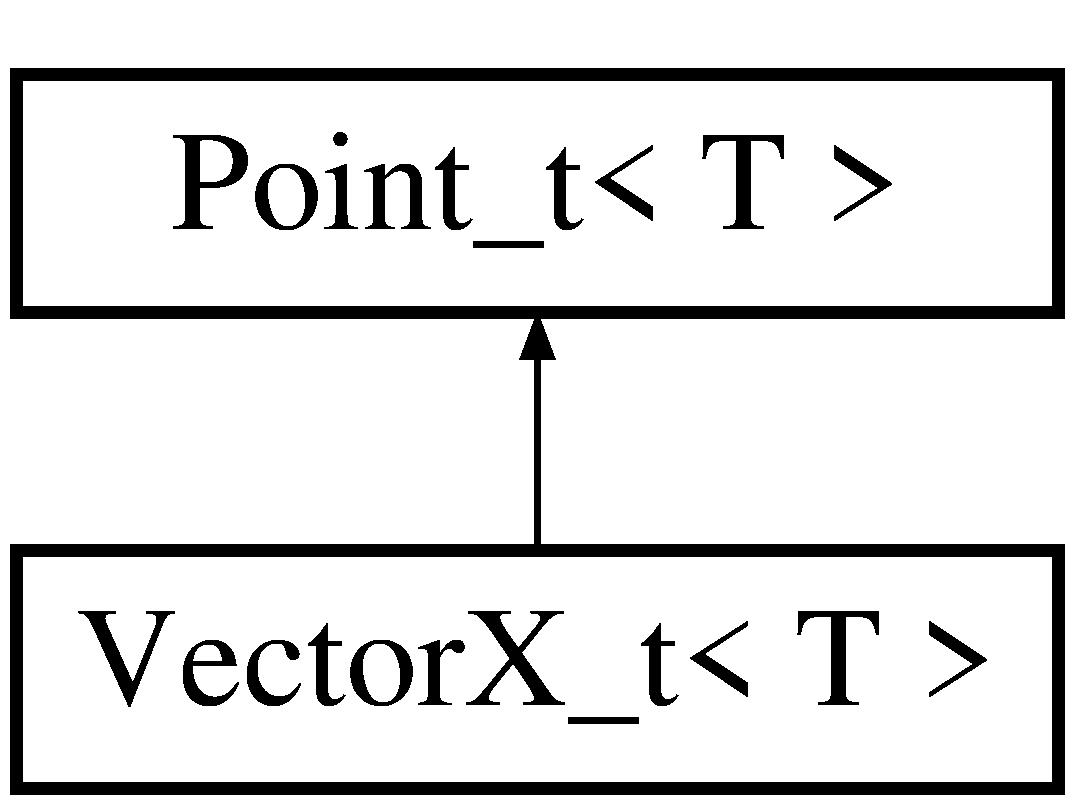
\includegraphics[height=2.000000cm]{class_point__t}
\end{center}
\end{figure}
\subsection*{Public Member Functions}
\begin{DoxyCompactItemize}
\item 
\hyperlink{class_point__t_a6a0871ca8592da56fae8dd0fde4dcc5d}{Point\+\_\+t} ()
\begin{DoxyCompactList}\small\item\em This is the Point constructor. \end{DoxyCompactList}\item 
\hyperlink{class_point__t_a74da469bad09c76462acae8e1b5f1a28}{Point\+\_\+t} (T xx, T yy)
\begin{DoxyCompactList}\small\item\em This is the 2D Point constructor that creates coordinates instantly. \end{DoxyCompactList}\item 
\hyperlink{class_point__t_ae825adbedce7f428b150eaa5454469e0}{Point\+\_\+t} (T xx, T yy, T zz)
\begin{DoxyCompactList}\small\item\em This is the 3D Point constructor that creates coordinates instantly. \end{DoxyCompactList}\item 
virtual \hyperlink{class_point__t_ae05b28ed42a34a491fd8a2a94500b51f}{$\sim$\+Point\+\_\+t} ()
\begin{DoxyCompactList}\small\item\em This is the Point destructor. \end{DoxyCompactList}\item 
\hyperlink{class_point__t}{Point\+\_\+t}$<$ T $>$ \& \hyperlink{class_point__t_abd0017d51000570cf8c5b071ef37aeb4}{operator+=} (const \hyperlink{class_point__t}{Point\+\_\+t}$<$ T $>$ \&rhs)
\begin{DoxyCompactList}\small\item\em returns the sum of two Points \end{DoxyCompactList}\item 
\hyperlink{class_point__t}{Point\+\_\+t}$<$ T $>$ \hyperlink{class_point__t_afac8b7bed8c8b0f6b5bcbbf3ae1362d9}{operator+} (const \hyperlink{class_point__t}{Point\+\_\+t}$<$ T $>$ \&rhs) const
\begin{DoxyCompactList}\small\item\em returns the sum of two Points \end{DoxyCompactList}\item 
\hyperlink{class_point__t}{Point\+\_\+t}$<$ T $>$ \& \hyperlink{class_point__t_a510c1649a1ff3b46bb602a48de37d7c0}{operator-\/=} (const \hyperlink{class_point__t}{Point\+\_\+t}$<$ T $>$ \&rhs)
\begin{DoxyCompactList}\small\item\em returns the difference between two Points \end{DoxyCompactList}\item 
\hyperlink{class_point__t}{Point\+\_\+t}$<$ T $>$ \hyperlink{class_point__t_ab20b4b331780f76392d465f498ca14e1}{operator-\/} (const \hyperlink{class_point__t}{Point\+\_\+t}$<$ T $>$ \&rhs) const
\begin{DoxyCompactList}\small\item\em returns the difference between two Points \end{DoxyCompactList}\item 
\hyperlink{class_point__t}{Point\+\_\+t}$<$ T $>$ \& \hyperlink{class_point__t_aefb9c2d617458a15d475690641e51b37}{operator$\ast$=} (const \hyperlink{class_point__t}{Point\+\_\+t}$<$ T $>$ \&rhs)
\begin{DoxyCompactList}\small\item\em returns the product of two Points \end{DoxyCompactList}\item 
\hyperlink{class_point__t}{Point\+\_\+t}$<$ T $>$ \hyperlink{class_point__t_a56b84bb4471a147a920444370b5bd9bc}{operator$\ast$} (const \hyperlink{class_point__t}{Point\+\_\+t}$<$ T $>$ \&rhs) const
\begin{DoxyCompactList}\small\item\em returns the product of two Points \end{DoxyCompactList}\item 
\hyperlink{class_point__t}{Point\+\_\+t}$<$ T $>$ \& \hyperlink{class_point__t_a7d548221c6fbe6401682052a5121aa9b}{operator/=} (const \hyperlink{class_point__t}{Point\+\_\+t}$<$ T $>$ \&rhs)
\begin{DoxyCompactList}\small\item\em returns the quotient of two Points \end{DoxyCompactList}\item 
\hyperlink{class_point__t}{Point\+\_\+t}$<$ T $>$ \hyperlink{class_point__t_a8ee1a27bc0d6386c7af20006956cab41}{operator/} (const \hyperlink{class_point__t}{Point\+\_\+t}$<$ T $>$ \&rhs) const
\begin{DoxyCompactList}\small\item\em returns the quotient of two Points \end{DoxyCompactList}\item 
\hyperlink{class_point__t}{Point\+\_\+t}$<$ T $>$ \& \hyperlink{class_point__t_adf6b36a63ecb3250ee9f35f1611e9393}{operator+=} (const T rhs)
\begin{DoxyCompactList}\small\item\em returns the sum of the Point and any number \end{DoxyCompactList}\item 
\hyperlink{class_point__t}{Point\+\_\+t}$<$ T $>$ \hyperlink{class_point__t_a18aa50064d17f83d4880ecafbc1cc115}{operator+} (const T rhs) const
\begin{DoxyCompactList}\small\item\em returns the sum of the Point and any number \end{DoxyCompactList}\item 
\hyperlink{class_point__t}{Point\+\_\+t}$<$ T $>$ \& \hyperlink{class_point__t_a52e5fc5e911f05b8e88fd918110dd502}{operator-\/=} (const T rhs)
\begin{DoxyCompactList}\small\item\em returns the difference of the Point and any number \end{DoxyCompactList}\item 
\hyperlink{class_point__t}{Point\+\_\+t}$<$ T $>$ \hyperlink{class_point__t_a6c180a0384480acf4929b75557d96748}{operator-\/} (const T rhs) const
\begin{DoxyCompactList}\small\item\em returns the difference of the Point and any number \end{DoxyCompactList}\item 
\hyperlink{class_point__t}{Point\+\_\+t}$<$ T $>$ \& \hyperlink{class_point__t_a0671ae26709b67542a902f4cbf1e2102}{operator$\ast$=} (const T rhs)
\begin{DoxyCompactList}\small\item\em returns the product of the Point and any number \end{DoxyCompactList}\item 
\hyperlink{class_point__t}{Point\+\_\+t}$<$ T $>$ \hyperlink{class_point__t_a6e2924110e74cc78027171765fb3eb84}{operator$\ast$} (const T rhs) const
\begin{DoxyCompactList}\small\item\em returns the product of the Point and any number \end{DoxyCompactList}\item 
\hyperlink{class_point__t}{Point\+\_\+t}$<$ T $>$ \& \hyperlink{class_point__t_a9035ca1de1358b7447d1c04a00c0b08e}{operator/=} (const T rhs)
\begin{DoxyCompactList}\small\item\em returns the quotient of the Point and any number \end{DoxyCompactList}\item 
\hyperlink{class_point__t}{Point\+\_\+t}$<$ T $>$ \hyperlink{class_point__t_ac7987146c54aa27b05399048598634c3}{operator/} (const T rhs) const
\begin{DoxyCompactList}\small\item\em returns the quotient of the Point and any number \end{DoxyCompactList}\item 
bool \hyperlink{class_point__t_aa9e7b08f004641102956f486c18e79b7}{operator==} (const \hyperlink{class_point__t}{Point\+\_\+t}$<$ T $>$ \&other) const
\begin{DoxyCompactList}\small\item\em Overloads the == operator. \end{DoxyCompactList}\item 
bool \hyperlink{class_point__t_aa5f770c4e0b7e3fe1e426fdebc4cd0f9}{operator!=} (const \hyperlink{class_point__t}{Point\+\_\+t}$<$ T $>$ \&other) const
\begin{DoxyCompactList}\small\item\em Overloads the != operator. \end{DoxyCompactList}\end{DoxyCompactItemize}
\subsection*{Public Attributes}
\begin{DoxyCompactItemize}
\item 
T \hyperlink{class_point__t_add0b296463fdccbde77953e480ae3d2d}{x}
\begin{DoxyCompactList}\small\item\em The x value of the Point. \end{DoxyCompactList}\item 
T \hyperlink{class_point__t_a2c1d504b00b0cf59edd07ad7611bbfde}{y}
\begin{DoxyCompactList}\small\item\em The y value of the Point. \end{DoxyCompactList}\item 
T \hyperlink{class_point__t_a7480dcfc81f5cf2eff6434da05b26c18}{z}
\begin{DoxyCompactList}\small\item\em The z value of the Point. \end{DoxyCompactList}\end{DoxyCompactItemize}


\subsection{Detailed Description}
\subsubsection*{template$<$class T$>$\newline
class Point\+\_\+t$<$ T $>$}

The \hyperlink{class_point__t}{Point\+\_\+t} class is a helper class that makes it easier to define points in space. 

\subsection{Constructor \& Destructor Documentation}
\mbox{\Hypertarget{class_point__t_a6a0871ca8592da56fae8dd0fde4dcc5d}\label{class_point__t_a6a0871ca8592da56fae8dd0fde4dcc5d}} 
\index{Point\+\_\+t@{Point\+\_\+t}!Point\+\_\+t@{Point\+\_\+t}}
\index{Point\+\_\+t@{Point\+\_\+t}!Point\+\_\+t@{Point\+\_\+t}}
\subsubsection{\texorpdfstring{Point\+\_\+t()}{Point\_t()}\hspace{0.1cm}{\footnotesize\ttfamily [1/3]}}
{\footnotesize\ttfamily template$<$class T $>$ \\
\hyperlink{class_point__t}{Point\+\_\+t}$<$ T $>$\+::\hyperlink{class_point__t}{Point\+\_\+t} (\begin{DoxyParamCaption}{ }\end{DoxyParamCaption})}



This is the Point constructor. 

It creates a Point at 0,0,0 \mbox{\Hypertarget{class_point__t_a74da469bad09c76462acae8e1b5f1a28}\label{class_point__t_a74da469bad09c76462acae8e1b5f1a28}} 
\index{Point\+\_\+t@{Point\+\_\+t}!Point\+\_\+t@{Point\+\_\+t}}
\index{Point\+\_\+t@{Point\+\_\+t}!Point\+\_\+t@{Point\+\_\+t}}
\subsubsection{\texorpdfstring{Point\+\_\+t()}{Point\_t()}\hspace{0.1cm}{\footnotesize\ttfamily [2/3]}}
{\footnotesize\ttfamily template$<$class T $>$ \\
\hyperlink{class_point__t}{Point\+\_\+t}$<$ T $>$\+::\hyperlink{class_point__t}{Point\+\_\+t} (\begin{DoxyParamCaption}\item[{T}]{xx,  }\item[{T}]{yy }\end{DoxyParamCaption})}



This is the 2D Point constructor that creates coordinates instantly. 


\begin{DoxyParams}{Parameters}
{\em xx} & The x value of the Point. \\
\hline
{\em yy} & The y value of the Point. \\
\hline
\end{DoxyParams}
\mbox{\Hypertarget{class_point__t_ae825adbedce7f428b150eaa5454469e0}\label{class_point__t_ae825adbedce7f428b150eaa5454469e0}} 
\index{Point\+\_\+t@{Point\+\_\+t}!Point\+\_\+t@{Point\+\_\+t}}
\index{Point\+\_\+t@{Point\+\_\+t}!Point\+\_\+t@{Point\+\_\+t}}
\subsubsection{\texorpdfstring{Point\+\_\+t()}{Point\_t()}\hspace{0.1cm}{\footnotesize\ttfamily [3/3]}}
{\footnotesize\ttfamily template$<$class T $>$ \\
\hyperlink{class_point__t}{Point\+\_\+t}$<$ T $>$\+::\hyperlink{class_point__t}{Point\+\_\+t} (\begin{DoxyParamCaption}\item[{T}]{xx,  }\item[{T}]{yy,  }\item[{T}]{zz }\end{DoxyParamCaption})}



This is the 3D Point constructor that creates coordinates instantly. 


\begin{DoxyParams}{Parameters}
{\em xx} & The x value of the Point. \\
\hline
{\em yy} & The y value of the Point. \\
\hline
{\em zz} & The z value of the Point. \\
\hline
\end{DoxyParams}
\mbox{\Hypertarget{class_point__t_ae05b28ed42a34a491fd8a2a94500b51f}\label{class_point__t_ae05b28ed42a34a491fd8a2a94500b51f}} 
\index{Point\+\_\+t@{Point\+\_\+t}!````~Point\+\_\+t@{$\sim$\+Point\+\_\+t}}
\index{````~Point\+\_\+t@{$\sim$\+Point\+\_\+t}!Point\+\_\+t@{Point\+\_\+t}}
\subsubsection{\texorpdfstring{$\sim$\+Point\+\_\+t()}{~Point\_t()}}
{\footnotesize\ttfamily template$<$class T $>$ \\
\hyperlink{class_point__t}{Point\+\_\+t}$<$ T $>$\+::$\sim$\hyperlink{class_point__t}{Point\+\_\+t} (\begin{DoxyParamCaption}{ }\end{DoxyParamCaption})\hspace{0.3cm}{\ttfamily [virtual]}}



This is the Point destructor. 

It cleans up the Point. 

\subsection{Member Function Documentation}
\mbox{\Hypertarget{class_point__t_aa5f770c4e0b7e3fe1e426fdebc4cd0f9}\label{class_point__t_aa5f770c4e0b7e3fe1e426fdebc4cd0f9}} 
\index{Point\+\_\+t@{Point\+\_\+t}!operator"!=@{operator"!=}}
\index{operator"!=@{operator"!=}!Point\+\_\+t@{Point\+\_\+t}}
\subsubsection{\texorpdfstring{operator"!=()}{operator!=()}}
{\footnotesize\ttfamily template$<$class T $>$ \\
bool \hyperlink{class_point__t}{Point\+\_\+t}$<$ T $>$\+::operator!= (\begin{DoxyParamCaption}\item[{const \hyperlink{class_point__t}{Point\+\_\+t}$<$ T $>$ \&}]{other }\end{DoxyParamCaption}) const}



Overloads the != operator. 


\begin{DoxyParams}{Parameters}
{\em other} & The Point to compare with\\
\hline
\end{DoxyParams}
\begin{DoxyReturn}{Returns}
boolean. true if Points are different 
\end{DoxyReturn}
\mbox{\Hypertarget{class_point__t_a56b84bb4471a147a920444370b5bd9bc}\label{class_point__t_a56b84bb4471a147a920444370b5bd9bc}} 
\index{Point\+\_\+t@{Point\+\_\+t}!operator$\ast$@{operator$\ast$}}
\index{operator$\ast$@{operator$\ast$}!Point\+\_\+t@{Point\+\_\+t}}
\subsubsection{\texorpdfstring{operator$\ast$()}{operator*()}\hspace{0.1cm}{\footnotesize\ttfamily [1/2]}}
{\footnotesize\ttfamily template$<$class T $>$ \\
\hyperlink{class_point__t}{Point\+\_\+t}$<$ T $>$ \hyperlink{class_point__t}{Point\+\_\+t}$<$ T $>$\+::operator$\ast$ (\begin{DoxyParamCaption}\item[{const \hyperlink{class_point__t}{Point\+\_\+t}$<$ T $>$ \&}]{rhs }\end{DoxyParamCaption}) const}



returns the product of two Points 


\begin{DoxyParams}{Parameters}
{\em rhs} & The Point to be multiplied\\
\hline
\end{DoxyParams}
\begin{DoxyReturn}{Returns}
the product of two Points 
\end{DoxyReturn}
\mbox{\Hypertarget{class_point__t_a6e2924110e74cc78027171765fb3eb84}\label{class_point__t_a6e2924110e74cc78027171765fb3eb84}} 
\index{Point\+\_\+t@{Point\+\_\+t}!operator$\ast$@{operator$\ast$}}
\index{operator$\ast$@{operator$\ast$}!Point\+\_\+t@{Point\+\_\+t}}
\subsubsection{\texorpdfstring{operator$\ast$()}{operator*()}\hspace{0.1cm}{\footnotesize\ttfamily [2/2]}}
{\footnotesize\ttfamily template$<$class T $>$ \\
\hyperlink{class_point__t}{Point\+\_\+t}$<$ T $>$ \hyperlink{class_point__t}{Point\+\_\+t}$<$ T $>$\+::operator$\ast$ (\begin{DoxyParamCaption}\item[{const T}]{rhs }\end{DoxyParamCaption}) const}



returns the product of the Point and any number 


\begin{DoxyParams}{Parameters}
{\em rhs} & The number to be multiplied\\
\hline
\end{DoxyParams}
\begin{DoxyReturn}{Returns}
the product of the Point and any number 
\end{DoxyReturn}
\mbox{\Hypertarget{class_point__t_aefb9c2d617458a15d475690641e51b37}\label{class_point__t_aefb9c2d617458a15d475690641e51b37}} 
\index{Point\+\_\+t@{Point\+\_\+t}!operator$\ast$=@{operator$\ast$=}}
\index{operator$\ast$=@{operator$\ast$=}!Point\+\_\+t@{Point\+\_\+t}}
\subsubsection{\texorpdfstring{operator$\ast$=()}{operator*=()}\hspace{0.1cm}{\footnotesize\ttfamily [1/2]}}
{\footnotesize\ttfamily template$<$class T $>$ \\
\hyperlink{class_point__t}{Point\+\_\+t}$<$ T $>$ \& \hyperlink{class_point__t}{Point\+\_\+t}$<$ T $>$\+::operator$\ast$= (\begin{DoxyParamCaption}\item[{const \hyperlink{class_point__t}{Point\+\_\+t}$<$ T $>$ \&}]{rhs }\end{DoxyParamCaption})}



returns the product of two Points 


\begin{DoxyParams}{Parameters}
{\em rhs} & The Point to be multiplied\\
\hline
\end{DoxyParams}
\begin{DoxyReturn}{Returns}
the product of two Points 
\end{DoxyReturn}
\mbox{\Hypertarget{class_point__t_a0671ae26709b67542a902f4cbf1e2102}\label{class_point__t_a0671ae26709b67542a902f4cbf1e2102}} 
\index{Point\+\_\+t@{Point\+\_\+t}!operator$\ast$=@{operator$\ast$=}}
\index{operator$\ast$=@{operator$\ast$=}!Point\+\_\+t@{Point\+\_\+t}}
\subsubsection{\texorpdfstring{operator$\ast$=()}{operator*=()}\hspace{0.1cm}{\footnotesize\ttfamily [2/2]}}
{\footnotesize\ttfamily template$<$class T $>$ \\
\hyperlink{class_point__t}{Point\+\_\+t}$<$ T $>$ \& \hyperlink{class_point__t}{Point\+\_\+t}$<$ T $>$\+::operator$\ast$= (\begin{DoxyParamCaption}\item[{const T}]{rhs }\end{DoxyParamCaption})}



returns the product of the Point and any number 


\begin{DoxyParams}{Parameters}
{\em rhs} & The number to be multiplied\\
\hline
\end{DoxyParams}
\begin{DoxyReturn}{Returns}
the product of the Point and any number 
\end{DoxyReturn}
\mbox{\Hypertarget{class_point__t_afac8b7bed8c8b0f6b5bcbbf3ae1362d9}\label{class_point__t_afac8b7bed8c8b0f6b5bcbbf3ae1362d9}} 
\index{Point\+\_\+t@{Point\+\_\+t}!operator+@{operator+}}
\index{operator+@{operator+}!Point\+\_\+t@{Point\+\_\+t}}
\subsubsection{\texorpdfstring{operator+()}{operator+()}\hspace{0.1cm}{\footnotesize\ttfamily [1/2]}}
{\footnotesize\ttfamily template$<$class T $>$ \\
\hyperlink{class_point__t}{Point\+\_\+t}$<$ T $>$ \hyperlink{class_point__t}{Point\+\_\+t}$<$ T $>$\+::operator+ (\begin{DoxyParamCaption}\item[{const \hyperlink{class_point__t}{Point\+\_\+t}$<$ T $>$ \&}]{rhs }\end{DoxyParamCaption}) const}



returns the sum of two Points 


\begin{DoxyParams}{Parameters}
{\em rhs} & The Point to be added\\
\hline
\end{DoxyParams}
\begin{DoxyReturn}{Returns}
the sum of two Points 
\end{DoxyReturn}
\mbox{\Hypertarget{class_point__t_a18aa50064d17f83d4880ecafbc1cc115}\label{class_point__t_a18aa50064d17f83d4880ecafbc1cc115}} 
\index{Point\+\_\+t@{Point\+\_\+t}!operator+@{operator+}}
\index{operator+@{operator+}!Point\+\_\+t@{Point\+\_\+t}}
\subsubsection{\texorpdfstring{operator+()}{operator+()}\hspace{0.1cm}{\footnotesize\ttfamily [2/2]}}
{\footnotesize\ttfamily template$<$class T $>$ \\
\hyperlink{class_point__t}{Point\+\_\+t}$<$ T $>$ \hyperlink{class_point__t}{Point\+\_\+t}$<$ T $>$\+::operator+ (\begin{DoxyParamCaption}\item[{const T}]{rhs }\end{DoxyParamCaption}) const}



returns the sum of the Point and any number 


\begin{DoxyParams}{Parameters}
{\em rhs} & The number to be multiplied\\
\hline
\end{DoxyParams}
\begin{DoxyReturn}{Returns}
the sum of the Point and any number 
\end{DoxyReturn}
\mbox{\Hypertarget{class_point__t_abd0017d51000570cf8c5b071ef37aeb4}\label{class_point__t_abd0017d51000570cf8c5b071ef37aeb4}} 
\index{Point\+\_\+t@{Point\+\_\+t}!operator+=@{operator+=}}
\index{operator+=@{operator+=}!Point\+\_\+t@{Point\+\_\+t}}
\subsubsection{\texorpdfstring{operator+=()}{operator+=()}\hspace{0.1cm}{\footnotesize\ttfamily [1/2]}}
{\footnotesize\ttfamily template$<$class T $>$ \\
\hyperlink{class_point__t}{Point\+\_\+t}$<$ T $>$ \& \hyperlink{class_point__t}{Point\+\_\+t}$<$ T $>$\+::operator+= (\begin{DoxyParamCaption}\item[{const \hyperlink{class_point__t}{Point\+\_\+t}$<$ T $>$ \&}]{rhs }\end{DoxyParamCaption})}



returns the sum of two Points 


\begin{DoxyParams}{Parameters}
{\em rhs} & The Point to be added\\
\hline
\end{DoxyParams}
\begin{DoxyReturn}{Returns}
the sum of two Points 
\end{DoxyReturn}
\mbox{\Hypertarget{class_point__t_adf6b36a63ecb3250ee9f35f1611e9393}\label{class_point__t_adf6b36a63ecb3250ee9f35f1611e9393}} 
\index{Point\+\_\+t@{Point\+\_\+t}!operator+=@{operator+=}}
\index{operator+=@{operator+=}!Point\+\_\+t@{Point\+\_\+t}}
\subsubsection{\texorpdfstring{operator+=()}{operator+=()}\hspace{0.1cm}{\footnotesize\ttfamily [2/2]}}
{\footnotesize\ttfamily template$<$class T $>$ \\
\hyperlink{class_point__t}{Point\+\_\+t}$<$ T $>$ \& \hyperlink{class_point__t}{Point\+\_\+t}$<$ T $>$\+::operator+= (\begin{DoxyParamCaption}\item[{const T}]{rhs }\end{DoxyParamCaption})}



returns the sum of the Point and any number 


\begin{DoxyParams}{Parameters}
{\em rhs} & The number to be added\\
\hline
\end{DoxyParams}
\begin{DoxyReturn}{Returns}
the sum of the Point and any number 
\end{DoxyReturn}
\mbox{\Hypertarget{class_point__t_ab20b4b331780f76392d465f498ca14e1}\label{class_point__t_ab20b4b331780f76392d465f498ca14e1}} 
\index{Point\+\_\+t@{Point\+\_\+t}!operator-\/@{operator-\/}}
\index{operator-\/@{operator-\/}!Point\+\_\+t@{Point\+\_\+t}}
\subsubsection{\texorpdfstring{operator-\/()}{operator-()}\hspace{0.1cm}{\footnotesize\ttfamily [1/2]}}
{\footnotesize\ttfamily template$<$class T $>$ \\
\hyperlink{class_point__t}{Point\+\_\+t}$<$ T $>$ \hyperlink{class_point__t}{Point\+\_\+t}$<$ T $>$\+::operator-\/ (\begin{DoxyParamCaption}\item[{const \hyperlink{class_point__t}{Point\+\_\+t}$<$ T $>$ \&}]{rhs }\end{DoxyParamCaption}) const}



returns the difference between two Points 


\begin{DoxyParams}{Parameters}
{\em rhs} & The Point to be subtracted\\
\hline
\end{DoxyParams}
\begin{DoxyReturn}{Returns}
the difference between two Points 
\end{DoxyReturn}
\mbox{\Hypertarget{class_point__t_a6c180a0384480acf4929b75557d96748}\label{class_point__t_a6c180a0384480acf4929b75557d96748}} 
\index{Point\+\_\+t@{Point\+\_\+t}!operator-\/@{operator-\/}}
\index{operator-\/@{operator-\/}!Point\+\_\+t@{Point\+\_\+t}}
\subsubsection{\texorpdfstring{operator-\/()}{operator-()}\hspace{0.1cm}{\footnotesize\ttfamily [2/2]}}
{\footnotesize\ttfamily template$<$class T $>$ \\
\hyperlink{class_point__t}{Point\+\_\+t}$<$ T $>$ \hyperlink{class_point__t}{Point\+\_\+t}$<$ T $>$\+::operator-\/ (\begin{DoxyParamCaption}\item[{const T}]{rhs }\end{DoxyParamCaption}) const}



returns the difference of the Point and any number 


\begin{DoxyParams}{Parameters}
{\em rhs} & The number to be subtracted\\
\hline
\end{DoxyParams}
\begin{DoxyReturn}{Returns}
the difference of the Point and any number 
\end{DoxyReturn}
\mbox{\Hypertarget{class_point__t_a510c1649a1ff3b46bb602a48de37d7c0}\label{class_point__t_a510c1649a1ff3b46bb602a48de37d7c0}} 
\index{Point\+\_\+t@{Point\+\_\+t}!operator-\/=@{operator-\/=}}
\index{operator-\/=@{operator-\/=}!Point\+\_\+t@{Point\+\_\+t}}
\subsubsection{\texorpdfstring{operator-\/=()}{operator-=()}\hspace{0.1cm}{\footnotesize\ttfamily [1/2]}}
{\footnotesize\ttfamily template$<$class T $>$ \\
\hyperlink{class_point__t}{Point\+\_\+t}$<$ T $>$ \& \hyperlink{class_point__t}{Point\+\_\+t}$<$ T $>$\+::operator-\/= (\begin{DoxyParamCaption}\item[{const \hyperlink{class_point__t}{Point\+\_\+t}$<$ T $>$ \&}]{rhs }\end{DoxyParamCaption})}



returns the difference between two Points 


\begin{DoxyParams}{Parameters}
{\em rhs} & The Point to be subtracted\\
\hline
\end{DoxyParams}
\begin{DoxyReturn}{Returns}
the difference between two Points 
\end{DoxyReturn}
\mbox{\Hypertarget{class_point__t_a52e5fc5e911f05b8e88fd918110dd502}\label{class_point__t_a52e5fc5e911f05b8e88fd918110dd502}} 
\index{Point\+\_\+t@{Point\+\_\+t}!operator-\/=@{operator-\/=}}
\index{operator-\/=@{operator-\/=}!Point\+\_\+t@{Point\+\_\+t}}
\subsubsection{\texorpdfstring{operator-\/=()}{operator-=()}\hspace{0.1cm}{\footnotesize\ttfamily [2/2]}}
{\footnotesize\ttfamily template$<$class T $>$ \\
\hyperlink{class_point__t}{Point\+\_\+t}$<$ T $>$ \& \hyperlink{class_point__t}{Point\+\_\+t}$<$ T $>$\+::operator-\/= (\begin{DoxyParamCaption}\item[{const T}]{rhs }\end{DoxyParamCaption})}



returns the difference of the Point and any number 


\begin{DoxyParams}{Parameters}
{\em rhs} & The number to be subtracted\\
\hline
\end{DoxyParams}
\begin{DoxyReturn}{Returns}
the difference between the Point and any number 
\end{DoxyReturn}
\mbox{\Hypertarget{class_point__t_a8ee1a27bc0d6386c7af20006956cab41}\label{class_point__t_a8ee1a27bc0d6386c7af20006956cab41}} 
\index{Point\+\_\+t@{Point\+\_\+t}!operator/@{operator/}}
\index{operator/@{operator/}!Point\+\_\+t@{Point\+\_\+t}}
\subsubsection{\texorpdfstring{operator/()}{operator/()}\hspace{0.1cm}{\footnotesize\ttfamily [1/2]}}
{\footnotesize\ttfamily template$<$class T $>$ \\
\hyperlink{class_point__t}{Point\+\_\+t}$<$ T $>$ \hyperlink{class_point__t}{Point\+\_\+t}$<$ T $>$\+::operator/ (\begin{DoxyParamCaption}\item[{const \hyperlink{class_point__t}{Point\+\_\+t}$<$ T $>$ \&}]{rhs }\end{DoxyParamCaption}) const}



returns the quotient of two Points 


\begin{DoxyParams}{Parameters}
{\em rhs} & The Point to be divided\\
\hline
\end{DoxyParams}
\begin{DoxyReturn}{Returns}
the quotient of two Points 
\end{DoxyReturn}
\mbox{\Hypertarget{class_point__t_ac7987146c54aa27b05399048598634c3}\label{class_point__t_ac7987146c54aa27b05399048598634c3}} 
\index{Point\+\_\+t@{Point\+\_\+t}!operator/@{operator/}}
\index{operator/@{operator/}!Point\+\_\+t@{Point\+\_\+t}}
\subsubsection{\texorpdfstring{operator/()}{operator/()}\hspace{0.1cm}{\footnotesize\ttfamily [2/2]}}
{\footnotesize\ttfamily template$<$class T $>$ \\
\hyperlink{class_point__t}{Point\+\_\+t}$<$ T $>$ \hyperlink{class_point__t}{Point\+\_\+t}$<$ T $>$\+::operator/ (\begin{DoxyParamCaption}\item[{const T}]{rhs }\end{DoxyParamCaption}) const}



returns the quotient of the Point and any number 


\begin{DoxyParams}{Parameters}
{\em rhs} & The number (divisor)\\
\hline
\end{DoxyParams}
\begin{DoxyReturn}{Returns}
the quotient of the Point and any number 
\end{DoxyReturn}
\mbox{\Hypertarget{class_point__t_a7d548221c6fbe6401682052a5121aa9b}\label{class_point__t_a7d548221c6fbe6401682052a5121aa9b}} 
\index{Point\+\_\+t@{Point\+\_\+t}!operator/=@{operator/=}}
\index{operator/=@{operator/=}!Point\+\_\+t@{Point\+\_\+t}}
\subsubsection{\texorpdfstring{operator/=()}{operator/=()}\hspace{0.1cm}{\footnotesize\ttfamily [1/2]}}
{\footnotesize\ttfamily template$<$class T $>$ \\
\hyperlink{class_point__t}{Point\+\_\+t}$<$ T $>$ \& \hyperlink{class_point__t}{Point\+\_\+t}$<$ T $>$\+::operator/= (\begin{DoxyParamCaption}\item[{const \hyperlink{class_point__t}{Point\+\_\+t}$<$ T $>$ \&}]{rhs }\end{DoxyParamCaption})}



returns the quotient of two Points 


\begin{DoxyParams}{Parameters}
{\em rhs} & The Point to be divided\\
\hline
\end{DoxyParams}
\begin{DoxyReturn}{Returns}
the quotient of two Points 
\end{DoxyReturn}
\mbox{\Hypertarget{class_point__t_a9035ca1de1358b7447d1c04a00c0b08e}\label{class_point__t_a9035ca1de1358b7447d1c04a00c0b08e}} 
\index{Point\+\_\+t@{Point\+\_\+t}!operator/=@{operator/=}}
\index{operator/=@{operator/=}!Point\+\_\+t@{Point\+\_\+t}}
\subsubsection{\texorpdfstring{operator/=()}{operator/=()}\hspace{0.1cm}{\footnotesize\ttfamily [2/2]}}
{\footnotesize\ttfamily template$<$class T $>$ \\
\hyperlink{class_point__t}{Point\+\_\+t}$<$ T $>$ \& \hyperlink{class_point__t}{Point\+\_\+t}$<$ T $>$\+::operator/= (\begin{DoxyParamCaption}\item[{const T}]{rhs }\end{DoxyParamCaption})}



returns the quotient of the Point and any number 


\begin{DoxyParams}{Parameters}
{\em rhs} & The number (divisor)\\
\hline
\end{DoxyParams}
\begin{DoxyReturn}{Returns}
the quotient of the Point and any number 
\end{DoxyReturn}
\mbox{\Hypertarget{class_point__t_aa9e7b08f004641102956f486c18e79b7}\label{class_point__t_aa9e7b08f004641102956f486c18e79b7}} 
\index{Point\+\_\+t@{Point\+\_\+t}!operator==@{operator==}}
\index{operator==@{operator==}!Point\+\_\+t@{Point\+\_\+t}}
\subsubsection{\texorpdfstring{operator==()}{operator==()}}
{\footnotesize\ttfamily template$<$class T $>$ \\
bool \hyperlink{class_point__t}{Point\+\_\+t}$<$ T $>$\+::operator== (\begin{DoxyParamCaption}\item[{const \hyperlink{class_point__t}{Point\+\_\+t}$<$ T $>$ \&}]{other }\end{DoxyParamCaption}) const}



Overloads the == operator. 


\begin{DoxyParams}{Parameters}
{\em other} & The Point to compare with\\
\hline
\end{DoxyParams}
\begin{DoxyReturn}{Returns}
boolean. true if Points are the same 
\end{DoxyReturn}


\subsection{Member Data Documentation}
\mbox{\Hypertarget{class_point__t_add0b296463fdccbde77953e480ae3d2d}\label{class_point__t_add0b296463fdccbde77953e480ae3d2d}} 
\index{Point\+\_\+t@{Point\+\_\+t}!x@{x}}
\index{x@{x}!Point\+\_\+t@{Point\+\_\+t}}
\subsubsection{\texorpdfstring{x}{x}}
{\footnotesize\ttfamily template$<$class T$>$ \\
\hyperlink{class_point__t}{Point\+\_\+t}$<$ T $>$\+::x}



The x value of the Point. 

This is a value on the horizontal axis.

The x value of the Point. \mbox{\Hypertarget{class_point__t_a2c1d504b00b0cf59edd07ad7611bbfde}\label{class_point__t_a2c1d504b00b0cf59edd07ad7611bbfde}} 
\index{Point\+\_\+t@{Point\+\_\+t}!y@{y}}
\index{y@{y}!Point\+\_\+t@{Point\+\_\+t}}
\subsubsection{\texorpdfstring{y}{y}}
{\footnotesize\ttfamily template$<$class T$>$ \\
\hyperlink{class_point__t}{Point\+\_\+t}$<$ T $>$\+::y}



The y value of the Point. 

This is a value on the vertical axis.

The y value of the Point. \mbox{\Hypertarget{class_point__t_a7480dcfc81f5cf2eff6434da05b26c18}\label{class_point__t_a7480dcfc81f5cf2eff6434da05b26c18}} 
\index{Point\+\_\+t@{Point\+\_\+t}!z@{z}}
\index{z@{z}!Point\+\_\+t@{Point\+\_\+t}}
\subsubsection{\texorpdfstring{z}{z}}
{\footnotesize\ttfamily template$<$class T$>$ \\
\hyperlink{class_point__t}{Point\+\_\+t}$<$ T $>$\+::z}



The z value of the Point. 

This is a value on the depth axis.

The z value of the Point. 

The documentation for this class was generated from the following file\+:\begin{DoxyCompactItemize}
\item 
\hyperlink{pointx_8h}{pointx.\+h}\end{DoxyCompactItemize}

\hypertarget{class_polar__t}{}\section{Polar\+\_\+t$<$ T $>$ Class Template Reference}
\label{class_polar__t}\index{Polar\+\_\+t$<$ T $>$@{Polar\+\_\+t$<$ T $>$}}


Polar (to Cartesian) coordinates helper class.  




{\ttfamily \#include $<$vectorx.\+h$>$}

\subsection*{Public Member Functions}
\begin{DoxyCompactItemize}
\item 
\mbox{\Hypertarget{class_polar__t_a4e6f79af5d5419c4d48a9b91a8743889}\label{class_polar__t_a4e6f79af5d5419c4d48a9b91a8743889}} 
\hyperlink{class_polar__t_a4e6f79af5d5419c4d48a9b91a8743889}{Polar\+\_\+t} ()
\begin{DoxyCompactList}\small\item\em Default Polar\+\_\+t$<$\+T$>$ constructor. \end{DoxyCompactList}\item 
\hyperlink{class_polar__t_a862fc0e18df7dad1470152e6ef2bd340}{Polar\+\_\+t} (T a, T r)
\begin{DoxyCompactList}\small\item\em Overloaded Polar\+\_\+t$<$\+T$>$ constructor. \end{DoxyCompactList}\item 
const \hyperlink{class_vector_x__t}{Vector\+X\+\_\+t}$<$ T $>$ \hyperlink{class_polar__t_aa4f91bf6479b2d2cefb22d79de8e1d42}{cartesian} () const
\begin{DoxyCompactList}\small\item\em Get the Cartesian coordinates of this \hyperlink{class_polar__t}{Polar\+\_\+t}. \end{DoxyCompactList}\item 
\hyperlink{class_polar__t}{Polar\+\_\+t}$<$ T $>$ \hyperlink{class_polar__t_a7a7ea302869a50342c010083943a2dbc}{from\+Cartesian} (const \hyperlink{class_vector_x__t}{Vector\+X\+\_\+t}$<$ T $>$ \&vec)
\begin{DoxyCompactList}\small\item\em Set this Polar from a \hyperlink{class_vector_x__t}{Vector\+X\+\_\+t}. \end{DoxyCompactList}\item 
\hyperlink{class_polar__t}{Polar\+\_\+t}$<$ T $>$ \hyperlink{class_polar__t_a18fa5c39eddf7f3554ddcec7ea95eb27}{from\+Cartesian} (T x, T y)
\begin{DoxyCompactList}\small\item\em Set this Polar from an x and y. \end{DoxyCompactList}\end{DoxyCompactItemize}
\subsection*{Public Attributes}
\begin{DoxyCompactItemize}
\item 
\mbox{\Hypertarget{class_polar__t_a97c5268b13511ac64a7650adc36554cb}\label{class_polar__t_a97c5268b13511ac64a7650adc36554cb}} 
T \hyperlink{class_polar__t_a97c5268b13511ac64a7650adc36554cb}{angle}
\begin{DoxyCompactList}\small\item\em angle of \hyperlink{class_polar__t}{Polar\+\_\+t} \end{DoxyCompactList}\item 
\mbox{\Hypertarget{class_polar__t_a2745dabb07096cd7360d88492e2d7eff}\label{class_polar__t_a2745dabb07096cd7360d88492e2d7eff}} 
T \hyperlink{class_polar__t_a2745dabb07096cd7360d88492e2d7eff}{radius}
\begin{DoxyCompactList}\small\item\em radius of \hyperlink{class_polar__t}{Polar\+\_\+t} \end{DoxyCompactList}\end{DoxyCompactItemize}


\subsection{Detailed Description}
\subsubsection*{template$<$class T$>$\newline
class Polar\+\_\+t$<$ T $>$}

Polar (to Cartesian) coordinates helper class. 

Usage\+: 
\begin{DoxyCode}
\hyperlink{class_vector_x__t}{Vector2} vec = \hyperlink{vectorx_8h_a599dfa361f200f3bfcf0dbe7aa2cd5ab}{Vector2}(4, 3);
std::cout << vec.\hyperlink{class_vector_x__t_a7e497c0abad76724767e78644ff91e35}{getAngle}()*\hyperlink{vectorx_8h_ad04f332238d224f48f547923ee6d3029}{RAD\_TO\_DEG} << std::endl; \textcolor{comment}{// 36.8699}
std::cout << vec.\hyperlink{class_vector_x__t_aa1548451f4620694a671d9b15be69ba2}{getLength}() << std::endl; \textcolor{comment}{// 5.0}

\hyperlink{class_polar__t}{Polar} p = \hyperlink{vectorx_8h_ae6dadb7c8827f4e57f3a883839948fec}{Polar}(36.8699*\hyperlink{vectorx_8h_aab4087f865137a540e6885dda23341cc}{DEG\_TO\_RAD}, 5.0f);
\hyperlink{class_vector_x__t}{Vector2} velocity = p.\hyperlink{class_polar__t_aa4f91bf6479b2d2cefb22d79de8e1d42}{cartesian}();
std::cout << velocity << std::endl; \textcolor{comment}{// (4, 3)}
\end{DoxyCode}
 

\subsection{Constructor \& Destructor Documentation}
\mbox{\Hypertarget{class_polar__t_a862fc0e18df7dad1470152e6ef2bd340}\label{class_polar__t_a862fc0e18df7dad1470152e6ef2bd340}} 
\index{Polar\+\_\+t@{Polar\+\_\+t}!Polar\+\_\+t@{Polar\+\_\+t}}
\index{Polar\+\_\+t@{Polar\+\_\+t}!Polar\+\_\+t@{Polar\+\_\+t}}
\subsubsection{\texorpdfstring{Polar\+\_\+t()}{Polar\_t()}}
{\footnotesize\ttfamily template$<$class T $>$ \\
\hyperlink{class_polar__t}{Polar\+\_\+t}$<$ T $>$\+::\hyperlink{class_polar__t}{Polar\+\_\+t} (\begin{DoxyParamCaption}\item[{T}]{a,  }\item[{T}]{r }\end{DoxyParamCaption})}



Overloaded Polar\+\_\+t$<$\+T$>$ constructor. 


\begin{DoxyParams}{Parameters}
{\em a} & angle \\
\hline
{\em r} & radius \\
\hline
\end{DoxyParams}


\subsection{Member Function Documentation}
\mbox{\Hypertarget{class_polar__t_aa4f91bf6479b2d2cefb22d79de8e1d42}\label{class_polar__t_aa4f91bf6479b2d2cefb22d79de8e1d42}} 
\index{Polar\+\_\+t@{Polar\+\_\+t}!cartesian@{cartesian}}
\index{cartesian@{cartesian}!Polar\+\_\+t@{Polar\+\_\+t}}
\subsubsection{\texorpdfstring{cartesian()}{cartesian()}}
{\footnotesize\ttfamily template$<$class T $>$ \\
const \hyperlink{class_vector_x__t}{Vector\+X\+\_\+t}$<$ T $>$ \hyperlink{class_polar__t}{Polar\+\_\+t}$<$ T $>$\+::cartesian (\begin{DoxyParamCaption}{ }\end{DoxyParamCaption}) const}



Get the Cartesian coordinates of this \hyperlink{class_polar__t}{Polar\+\_\+t}. 

\begin{DoxyReturn}{Returns}
Vector\+X\+\_\+t$<$\+T$>$ A \hyperlink{class_vector_x__t}{Vector\+X\+\_\+t} with the cartesian coordinates of this \hyperlink{class_polar__t}{Polar\+\_\+t} 
\end{DoxyReturn}
\mbox{\Hypertarget{class_polar__t_a7a7ea302869a50342c010083943a2dbc}\label{class_polar__t_a7a7ea302869a50342c010083943a2dbc}} 
\index{Polar\+\_\+t@{Polar\+\_\+t}!from\+Cartesian@{from\+Cartesian}}
\index{from\+Cartesian@{from\+Cartesian}!Polar\+\_\+t@{Polar\+\_\+t}}
\subsubsection{\texorpdfstring{from\+Cartesian()}{fromCartesian()}\hspace{0.1cm}{\footnotesize\ttfamily [1/2]}}
{\footnotesize\ttfamily template$<$class T $>$ \\
\hyperlink{class_polar__t}{Polar\+\_\+t}$<$ T $>$ \hyperlink{class_polar__t}{Polar\+\_\+t}$<$ T $>$\+::from\+Cartesian (\begin{DoxyParamCaption}\item[{const \hyperlink{class_vector_x__t}{Vector\+X\+\_\+t}$<$ T $>$ \&}]{vec }\end{DoxyParamCaption})}



Set this Polar from a \hyperlink{class_vector_x__t}{Vector\+X\+\_\+t}. 

\begin{DoxyReturn}{Returns}
Polar\+\_\+t$<$\+T$>$ 
\end{DoxyReturn}
\mbox{\Hypertarget{class_polar__t_a18fa5c39eddf7f3554ddcec7ea95eb27}\label{class_polar__t_a18fa5c39eddf7f3554ddcec7ea95eb27}} 
\index{Polar\+\_\+t@{Polar\+\_\+t}!from\+Cartesian@{from\+Cartesian}}
\index{from\+Cartesian@{from\+Cartesian}!Polar\+\_\+t@{Polar\+\_\+t}}
\subsubsection{\texorpdfstring{from\+Cartesian()}{fromCartesian()}\hspace{0.1cm}{\footnotesize\ttfamily [2/2]}}
{\footnotesize\ttfamily template$<$class T $>$ \\
\hyperlink{class_polar__t}{Polar\+\_\+t}$<$ T $>$ \hyperlink{class_polar__t}{Polar\+\_\+t}$<$ T $>$\+::from\+Cartesian (\begin{DoxyParamCaption}\item[{T}]{x,  }\item[{T}]{y }\end{DoxyParamCaption})}



Set this Polar from an x and y. 

\begin{DoxyReturn}{Returns}
Polar\+\_\+t$<$\+T$>$ 
\end{DoxyReturn}


The documentation for this class was generated from the following file\+:\begin{DoxyCompactItemize}
\item 
\hyperlink{vectorx_8h}{vectorx.\+h}\end{DoxyCompactItemize}

\hypertarget{class_renderer}{}\section{Renderer Class Reference}
\label{class_renderer}\index{Renderer@{Renderer}}


The \hyperlink{class_renderer}{Renderer} class renders meshes (vertices, normals, UV coordinates) from Sprites.  




{\ttfamily \#include $<$renderer.\+h$>$}

\subsection*{Public Member Functions}
\begin{DoxyCompactItemize}
\item 
\mbox{\Hypertarget{class_renderer_a7ebf46f54dab9905f79b80f7fddb76a6}\label{class_renderer_a7ebf46f54dab9905f79b80f7fddb76a6}} 
\hyperlink{class_renderer_a7ebf46f54dab9905f79b80f7fddb76a6}{Renderer} ()
\begin{DoxyCompactList}\small\item\em Constructor of the \hyperlink{class_renderer}{Renderer}. \end{DoxyCompactList}\item 
\mbox{\Hypertarget{class_renderer_afeee408862d5bd6255a6882d47e6d5cd}\label{class_renderer_afeee408862d5bd6255a6882d47e6d5cd}} 
virtual \hyperlink{class_renderer_afeee408862d5bd6255a6882d47e6d5cd}{$\sim$\+Renderer} ()
\begin{DoxyCompactList}\small\item\em Destructor of the \hyperlink{class_renderer}{Renderer}. \end{DoxyCompactList}\item 
int \hyperlink{class_renderer_a609f1ee6a2e5033035eb47636d0901ad}{init} ()
\begin{DoxyCompactList}\small\item\em Initialise the \hyperlink{class_renderer}{Renderer}. Create a Window with Open\+GL Context. \end{DoxyCompactList}\item 
void \hyperlink{class_renderer_a6dc601fc4faf3ab41bd212f6f31eaf89}{render\+Scene} (\hyperlink{class_scene}{Scene} $\ast$scene)
\begin{DoxyCompactList}\small\item\em Renders a \hyperlink{class_scene}{Scene} with all its children. \end{DoxyCompactList}\item 
G\+L\+F\+Wwindow $\ast$ \hyperlink{class_renderer_aeaa64bb33b48726eaf294827ac12bb18}{window} ()
\begin{DoxyCompactList}\small\item\em access the G\+L\+F\+Wwindow. \end{DoxyCompactList}\item 
void \hyperlink{class_renderer_a40b6ff3f5a306181f0ddc04e47462f41}{cleanup} ()
\begin{DoxyCompactList}\small\item\em cleanup (\+\_\+resman) \end{DoxyCompactList}\end{DoxyCompactItemize}


\subsection{Detailed Description}
The \hyperlink{class_renderer}{Renderer} class renders meshes (vertices, normals, UV coordinates) from Sprites. 

\subsection{Member Function Documentation}
\mbox{\Hypertarget{class_renderer_a40b6ff3f5a306181f0ddc04e47462f41}\label{class_renderer_a40b6ff3f5a306181f0ddc04e47462f41}} 
\index{Renderer@{Renderer}!cleanup@{cleanup}}
\index{cleanup@{cleanup}!Renderer@{Renderer}}
\subsubsection{\texorpdfstring{cleanup()}{cleanup()}}
{\footnotesize\ttfamily void Renderer\+::cleanup (\begin{DoxyParamCaption}{ }\end{DoxyParamCaption})}



cleanup (\+\_\+resman) 

\begin{DoxyReturn}{Returns}
void 
\end{DoxyReturn}
\mbox{\Hypertarget{class_renderer_a609f1ee6a2e5033035eb47636d0901ad}\label{class_renderer_a609f1ee6a2e5033035eb47636d0901ad}} 
\index{Renderer@{Renderer}!init@{init}}
\index{init@{init}!Renderer@{Renderer}}
\subsubsection{\texorpdfstring{init()}{init()}}
{\footnotesize\ttfamily int Renderer\+::init (\begin{DoxyParamCaption}{ }\end{DoxyParamCaption})}



Initialise the \hyperlink{class_renderer}{Renderer}. Create a Window with Open\+GL Context. 

\begin{DoxyReturn}{Returns}
int (0 when successful, -\/1 when errors occurred) 
\end{DoxyReturn}
\mbox{\Hypertarget{class_renderer_a6dc601fc4faf3ab41bd212f6f31eaf89}\label{class_renderer_a6dc601fc4faf3ab41bd212f6f31eaf89}} 
\index{Renderer@{Renderer}!render\+Scene@{render\+Scene}}
\index{render\+Scene@{render\+Scene}!Renderer@{Renderer}}
\subsubsection{\texorpdfstring{render\+Scene()}{renderScene()}}
{\footnotesize\ttfamily void Renderer\+::render\+Scene (\begin{DoxyParamCaption}\item[{\hyperlink{class_scene}{Scene} $\ast$}]{scene }\end{DoxyParamCaption})}



Renders a \hyperlink{class_scene}{Scene} with all its children. 


\begin{DoxyParams}{Parameters}
{\em scene} & The \hyperlink{class_scene}{Scene} that needs to be rendered \\
\hline
\end{DoxyParams}
\begin{DoxyReturn}{Returns}
void 
\end{DoxyReturn}
\mbox{\Hypertarget{class_renderer_aeaa64bb33b48726eaf294827ac12bb18}\label{class_renderer_aeaa64bb33b48726eaf294827ac12bb18}} 
\index{Renderer@{Renderer}!window@{window}}
\index{window@{window}!Renderer@{Renderer}}
\subsubsection{\texorpdfstring{window()}{window()}}
{\footnotesize\ttfamily G\+L\+F\+Wwindow$\ast$ Renderer\+::window (\begin{DoxyParamCaption}{ }\end{DoxyParamCaption})\hspace{0.3cm}{\ttfamily [inline]}}



access the G\+L\+F\+Wwindow. 

\begin{DoxyReturn}{Returns}
G\+L\+F\+Wwindow$\ast$ \+\_\+window 
\end{DoxyReturn}


The documentation for this class was generated from the following files\+:\begin{DoxyCompactItemize}
\item 
\hyperlink{renderer_8h}{renderer.\+h}\item 
renderer.\+cpp\end{DoxyCompactItemize}

\hypertarget{class_resource_manager}{}\section{Resource\+Manager Class Reference}
\label{class_resource_manager}\index{Resource\+Manager@{Resource\+Manager}}


The \hyperlink{class_resource_manager}{Resource\+Manager} class makes sure resources are loaded from disk only once.  




{\ttfamily \#include $<$resourcemanager.\+h$>$}

\subsection*{Public Member Functions}
\begin{DoxyCompactItemize}
\item 
\hyperlink{class_resource_manager_a3b32babd2e81909bbd90d7f2d566fadb}{Resource\+Manager} ()
\begin{DoxyCompactList}\small\item\em Constructor of the \hyperlink{class_resource_manager}{Resource\+Manager}. \end{DoxyCompactList}\item 
\mbox{\Hypertarget{class_resource_manager_a671c186e4630599e7e36d000c53eaf80}\label{class_resource_manager_a671c186e4630599e7e36d000c53eaf80}} 
virtual \hyperlink{class_resource_manager_a671c186e4630599e7e36d000c53eaf80}{$\sim$\+Resource\+Manager} ()
\begin{DoxyCompactList}\small\item\em Destructor of the \hyperlink{class_resource_manager}{Resource\+Manager}. \end{DoxyCompactList}\item 
\hyperlink{class_texture}{Texture} $\ast$ \hyperlink{class_resource_manager_a66f5436b2a1b78459f543e45ba5013eb}{get\+Texture} (const std\+::string \&filename, int filter, int wrap)
\begin{DoxyCompactList}\small\item\em get a \hyperlink{class_texture}{Texture} (from disk if need be) \end{DoxyCompactList}\item 
\hyperlink{class_mesh}{Mesh} $\ast$ \hyperlink{class_resource_manager_a83af97058447e2119fc870a405421e32}{get\+Sprite\+Mesh} (int width, int height, float pivotx, float pivoty, float uvwidth, float uvheight, int circle, int which)
\begin{DoxyCompactList}\small\item\em Generate a \hyperlink{class_sprite}{Sprite} \hyperlink{class_mesh}{Mesh}. \end{DoxyCompactList}\item 
\hyperlink{class_mesh}{Mesh} $\ast$ \hyperlink{class_resource_manager_ac6b7bc445bf9193e5791d80d74b07591}{get\+Line\+Mesh} (\hyperlink{class_line}{Line} $\ast$line)
\begin{DoxyCompactList}\small\item\em Generate a \hyperlink{class_line}{Line} \hyperlink{class_mesh}{Mesh}. \end{DoxyCompactList}\item 
\hyperlink{class_shader}{Shader} $\ast$ \hyperlink{class_resource_manager_ad4fba1143552a85ea52f864a1e445c25}{get\+Shader} (const std\+::string \&vs, const std\+::string \&fs)
\begin{DoxyCompactList}\small\item\em Get a \hyperlink{class_shader}{Shader} (from disk if need be) \end{DoxyCompactList}\item 
void \hyperlink{class_resource_manager_a027b7aa8171349b251ec46e4cc8ead56}{cleanup} ()
\begin{DoxyCompactList}\small\item\em clean up resources \end{DoxyCompactList}\end{DoxyCompactItemize}


\subsection{Detailed Description}
The \hyperlink{class_resource_manager}{Resource\+Manager} class makes sure resources are loaded from disk only once. 

\subsection{Constructor \& Destructor Documentation}
\mbox{\Hypertarget{class_resource_manager_a3b32babd2e81909bbd90d7f2d566fadb}\label{class_resource_manager_a3b32babd2e81909bbd90d7f2d566fadb}} 
\index{Resource\+Manager@{Resource\+Manager}!Resource\+Manager@{Resource\+Manager}}
\index{Resource\+Manager@{Resource\+Manager}!Resource\+Manager@{Resource\+Manager}}
\subsubsection{\texorpdfstring{Resource\+Manager()}{ResourceManager()}}
{\footnotesize\ttfamily Resource\+Manager\+::\+Resource\+Manager (\begin{DoxyParamCaption}{ }\end{DoxyParamCaption})}



Constructor of the \hyperlink{class_resource_manager}{Resource\+Manager}. 

This file is part of R\+T2D, a 2D Open\+GL framework.


\begin{DoxyItemize}
\item Copyright 2015 Rik Teerling \href{mailto:rik@onandoffables.com}{\tt rik@onandoffables.\+com}
\begin{DoxyItemize}
\item Initial commit 
\end{DoxyItemize}
\end{DoxyItemize}

\subsection{Member Function Documentation}
\mbox{\Hypertarget{class_resource_manager_a027b7aa8171349b251ec46e4cc8ead56}\label{class_resource_manager_a027b7aa8171349b251ec46e4cc8ead56}} 
\index{Resource\+Manager@{Resource\+Manager}!cleanup@{cleanup}}
\index{cleanup@{cleanup}!Resource\+Manager@{Resource\+Manager}}
\subsubsection{\texorpdfstring{cleanup()}{cleanup()}}
{\footnotesize\ttfamily void Resource\+Manager\+::cleanup (\begin{DoxyParamCaption}{ }\end{DoxyParamCaption})}



clean up resources 

\begin{DoxyReturn}{Returns}
void 
\end{DoxyReturn}
\mbox{\Hypertarget{class_resource_manager_ac6b7bc445bf9193e5791d80d74b07591}\label{class_resource_manager_ac6b7bc445bf9193e5791d80d74b07591}} 
\index{Resource\+Manager@{Resource\+Manager}!get\+Line\+Mesh@{get\+Line\+Mesh}}
\index{get\+Line\+Mesh@{get\+Line\+Mesh}!Resource\+Manager@{Resource\+Manager}}
\subsubsection{\texorpdfstring{get\+Line\+Mesh()}{getLineMesh()}}
{\footnotesize\ttfamily \hyperlink{class_mesh}{Mesh} $\ast$ Resource\+Manager\+::get\+Line\+Mesh (\begin{DoxyParamCaption}\item[{\hyperlink{class_line}{Line} $\ast$}]{line }\end{DoxyParamCaption})}



Generate a \hyperlink{class_line}{Line} \hyperlink{class_mesh}{Mesh}. 


\begin{DoxyParams}{Parameters}
{\em line} & pointer to a \hyperlink{class_line}{Line} \\
\hline
\end{DoxyParams}
\begin{DoxyReturn}{Returns}
Mesh$\ast$ a pointer to the generated \hyperlink{class_mesh}{Mesh} 
\end{DoxyReturn}
\mbox{\Hypertarget{class_resource_manager_ad4fba1143552a85ea52f864a1e445c25}\label{class_resource_manager_ad4fba1143552a85ea52f864a1e445c25}} 
\index{Resource\+Manager@{Resource\+Manager}!get\+Shader@{get\+Shader}}
\index{get\+Shader@{get\+Shader}!Resource\+Manager@{Resource\+Manager}}
\subsubsection{\texorpdfstring{get\+Shader()}{getShader()}}
{\footnotesize\ttfamily \hyperlink{class_shader}{Shader} $\ast$ Resource\+Manager\+::get\+Shader (\begin{DoxyParamCaption}\item[{const std\+::string \&}]{vs,  }\item[{const std\+::string \&}]{fs }\end{DoxyParamCaption})}



Get a \hyperlink{class_shader}{Shader} (from disk if need be) 


\begin{DoxyParams}{Parameters}
{\em vs} & the vertex \hyperlink{class_shader}{Shader} \\
\hline
{\em fs} & the fragment \hyperlink{class_shader}{Shader} (\textquotesingle{}pixelshader\textquotesingle{}) \\
\hline
\end{DoxyParams}
\begin{DoxyReturn}{Returns}
Shader$\ast$ a pointer to a \hyperlink{class_shader}{Shader} 
\end{DoxyReturn}
\mbox{\Hypertarget{class_resource_manager_a83af97058447e2119fc870a405421e32}\label{class_resource_manager_a83af97058447e2119fc870a405421e32}} 
\index{Resource\+Manager@{Resource\+Manager}!get\+Sprite\+Mesh@{get\+Sprite\+Mesh}}
\index{get\+Sprite\+Mesh@{get\+Sprite\+Mesh}!Resource\+Manager@{Resource\+Manager}}
\subsubsection{\texorpdfstring{get\+Sprite\+Mesh()}{getSpriteMesh()}}
{\footnotesize\ttfamily \hyperlink{class_mesh}{Mesh} $\ast$ Resource\+Manager\+::get\+Sprite\+Mesh (\begin{DoxyParamCaption}\item[{int}]{width,  }\item[{int}]{height,  }\item[{float}]{pivotx,  }\item[{float}]{pivoty,  }\item[{float}]{uvwidth,  }\item[{float}]{uvheight,  }\item[{int}]{circle,  }\item[{int}]{which }\end{DoxyParamCaption})}



Generate a \hyperlink{class_sprite}{Sprite} \hyperlink{class_mesh}{Mesh}. 


\begin{DoxyParams}{Parameters}
{\em width} & the width of the \hyperlink{class_sprite}{Sprite} \\
\hline
{\em height} & the height of the \hyperlink{class_sprite}{Sprite} \\
\hline
{\em pivotx} & the X component of the pivotpoint of the \hyperlink{class_sprite}{Sprite} \\
\hline
{\em pivoty} & the Y component of the pivotpoint of the \hyperlink{class_sprite}{Sprite} \\
\hline
{\em uvwidth} & the UV width of the Sprite\+Sheet \\
\hline
{\em uvheight} & the UV height of the Sprite\+Sheet \\
\hline
{\em circle} & generate custom \hyperlink{class_mesh}{Mesh} or Circle (0=square \hyperlink{class_sprite}{Sprite}, 6=hexagon) \\
\hline
{\em which} & if a segmentmesh, which segemnt to create (single triangle) \\
\hline
\end{DoxyParams}
\begin{DoxyReturn}{Returns}
Mesh$\ast$ a pointer to the generated \hyperlink{class_mesh}{Mesh} 
\end{DoxyReturn}
\mbox{\Hypertarget{class_resource_manager_a66f5436b2a1b78459f543e45ba5013eb}\label{class_resource_manager_a66f5436b2a1b78459f543e45ba5013eb}} 
\index{Resource\+Manager@{Resource\+Manager}!get\+Texture@{get\+Texture}}
\index{get\+Texture@{get\+Texture}!Resource\+Manager@{Resource\+Manager}}
\subsubsection{\texorpdfstring{get\+Texture()}{getTexture()}}
{\footnotesize\ttfamily \hyperlink{class_texture}{Texture} $\ast$ Resource\+Manager\+::get\+Texture (\begin{DoxyParamCaption}\item[{const std\+::string \&}]{filename,  }\item[{int}]{filter,  }\item[{int}]{wrap }\end{DoxyParamCaption})}



get a \hyperlink{class_texture}{Texture} (from disk if need be) 


\begin{DoxyParams}{Parameters}
{\em filename} & the path to the T\+GA file \\
\hline
{\em filter} & the filtering of the \hyperlink{class_texture}{Texture} \\
\hline
{\em wrap} & the UV wrapping of the \hyperlink{class_texture}{Texture} \\
\hline
\end{DoxyParams}
\begin{DoxyReturn}{Returns}
Texture$\ast$ a pointer to a \hyperlink{class_texture}{Texture}, created from an image file (.tga only). 
\end{DoxyReturn}


The documentation for this class was generated from the following files\+:\begin{DoxyCompactItemize}
\item 
\hyperlink{resourcemanager_8h}{resourcemanager.\+h}\item 
resourcemanager.\+cpp\end{DoxyCompactItemize}

\hypertarget{struct_r_g_b_a_color}{}\section{R\+G\+B\+A\+Color Struct Reference}
\label{struct_r_g_b_a_color}\index{R\+G\+B\+A\+Color@{R\+G\+B\+A\+Color}}


A 32 bit R\+G\+BA color.  




{\ttfamily \#include $<$color.\+h$>$}

\subsection*{Public Member Functions}
\begin{DoxyCompactItemize}
\item 
\mbox{\Hypertarget{struct_r_g_b_a_color_ac9d9ea70afb4ce5597d90b06f12b3d41}\label{struct_r_g_b_a_color_ac9d9ea70afb4ce5597d90b06f12b3d41}} 
\hyperlink{struct_r_g_b_a_color_ac9d9ea70afb4ce5597d90b06f12b3d41}{R\+G\+B\+A\+Color} ()
\begin{DoxyCompactList}\small\item\em constructor \end{DoxyCompactList}\item 
\hyperlink{struct_r_g_b_a_color_a40efdde5cc2f64bb3997256c7b89dbff}{R\+G\+B\+A\+Color} (uint8\+\_\+t red, uint8\+\_\+t green, uint8\+\_\+t blue, uint8\+\_\+t alpha)
\begin{DoxyCompactList}\small\item\em constructor \end{DoxyCompactList}\item 
\hyperlink{struct_r_g_b_a_color_a569aa1f50edef6490df126292387f432}{R\+G\+B\+A\+Color} (uint8\+\_\+t red, uint8\+\_\+t green, uint8\+\_\+t blue)
\begin{DoxyCompactList}\small\item\em constructor \end{DoxyCompactList}\item 
\hyperlink{struct_r_g_b_a_color_a62f554a0bc7a82d396f71f801dac624d}{R\+G\+B\+A\+Color} (uint32\+\_\+t color)
\begin{DoxyCompactList}\small\item\em constructor \end{DoxyCompactList}\item 
uint32\+\_\+t \hyperlink{struct_r_g_b_a_color_a9bbae2e2f28e388d589b83ab25f94b6a}{as\+Int} ()
\begin{DoxyCompactList}\small\item\em get color as a uint32\+\_\+t \end{DoxyCompactList}\item 
bool \hyperlink{struct_r_g_b_a_color_a8bad14391669eefbba155db49757b5c6}{operator==} (const \hyperlink{struct_r_g_b_a_color}{R\+G\+B\+A\+Color} \&rhs)
\begin{DoxyCompactList}\small\item\em == operator overloader \end{DoxyCompactList}\item 
bool \hyperlink{struct_r_g_b_a_color_a5e327a23436aa072a58003f0033729b1}{operator!=} (const \hyperlink{struct_r_g_b_a_color}{R\+G\+B\+A\+Color} \&rhs)
\begin{DoxyCompactList}\small\item\em != operator overloader \end{DoxyCompactList}\end{DoxyCompactItemize}
\subsection*{Public Attributes}
\begin{DoxyCompactItemize}
\item 
\mbox{\Hypertarget{struct_r_g_b_a_color_a575c7cb6c9ea4bf269d66c1ee7ae2901}\label{struct_r_g_b_a_color_a575c7cb6c9ea4bf269d66c1ee7ae2901}} 
uint8\+\_\+t \hyperlink{struct_r_g_b_a_color_a575c7cb6c9ea4bf269d66c1ee7ae2901}{r} = 255
\begin{DoxyCompactList}\small\item\em The red component of the color. \end{DoxyCompactList}\item 
\mbox{\Hypertarget{struct_r_g_b_a_color_a7d0de3f651397899480c902cbbba39c2}\label{struct_r_g_b_a_color_a7d0de3f651397899480c902cbbba39c2}} 
uint8\+\_\+t \hyperlink{struct_r_g_b_a_color_a7d0de3f651397899480c902cbbba39c2}{g} = 255
\begin{DoxyCompactList}\small\item\em The green component of the color. \end{DoxyCompactList}\item 
\mbox{\Hypertarget{struct_r_g_b_a_color_a1574ab45c8659742237c678a80ca00dc}\label{struct_r_g_b_a_color_a1574ab45c8659742237c678a80ca00dc}} 
uint8\+\_\+t \hyperlink{struct_r_g_b_a_color_a1574ab45c8659742237c678a80ca00dc}{b} = 255
\begin{DoxyCompactList}\small\item\em The blue component of the color. \end{DoxyCompactList}\item 
\mbox{\Hypertarget{struct_r_g_b_a_color_a594c214be1819bcd7f70b7246fb578f8}\label{struct_r_g_b_a_color_a594c214be1819bcd7f70b7246fb578f8}} 
uint8\+\_\+t \hyperlink{struct_r_g_b_a_color_a594c214be1819bcd7f70b7246fb578f8}{a} = 255
\begin{DoxyCompactList}\small\item\em The alpha component of the color. \end{DoxyCompactList}\end{DoxyCompactItemize}


\subsection{Detailed Description}
A 32 bit R\+G\+BA color. 

A struct that defines an R\+G\+BA \hyperlink{struct_color}{Color}. Each value is an uint8\+\_\+t (0-\/255). 

\subsection{Constructor \& Destructor Documentation}
\mbox{\Hypertarget{struct_r_g_b_a_color_a40efdde5cc2f64bb3997256c7b89dbff}\label{struct_r_g_b_a_color_a40efdde5cc2f64bb3997256c7b89dbff}} 
\index{R\+G\+B\+A\+Color@{R\+G\+B\+A\+Color}!R\+G\+B\+A\+Color@{R\+G\+B\+A\+Color}}
\index{R\+G\+B\+A\+Color@{R\+G\+B\+A\+Color}!R\+G\+B\+A\+Color@{R\+G\+B\+A\+Color}}
\subsubsection{\texorpdfstring{R\+G\+B\+A\+Color()}{RGBAColor()}\hspace{0.1cm}{\footnotesize\ttfamily [1/3]}}
{\footnotesize\ttfamily R\+G\+B\+A\+Color\+::\+R\+G\+B\+A\+Color (\begin{DoxyParamCaption}\item[{uint8\+\_\+t}]{red,  }\item[{uint8\+\_\+t}]{green,  }\item[{uint8\+\_\+t}]{blue,  }\item[{uint8\+\_\+t}]{alpha }\end{DoxyParamCaption})\hspace{0.3cm}{\ttfamily [inline]}}



constructor 


\begin{DoxyParams}{Parameters}
{\em red} & The red component of the color \\
\hline
{\em green} & The green component of the color \\
\hline
{\em blue} & The blue component of the color \\
\hline
{\em alpha} & The alpha component of the color \\
\hline
\end{DoxyParams}
\mbox{\Hypertarget{struct_r_g_b_a_color_a569aa1f50edef6490df126292387f432}\label{struct_r_g_b_a_color_a569aa1f50edef6490df126292387f432}} 
\index{R\+G\+B\+A\+Color@{R\+G\+B\+A\+Color}!R\+G\+B\+A\+Color@{R\+G\+B\+A\+Color}}
\index{R\+G\+B\+A\+Color@{R\+G\+B\+A\+Color}!R\+G\+B\+A\+Color@{R\+G\+B\+A\+Color}}
\subsubsection{\texorpdfstring{R\+G\+B\+A\+Color()}{RGBAColor()}\hspace{0.1cm}{\footnotesize\ttfamily [2/3]}}
{\footnotesize\ttfamily R\+G\+B\+A\+Color\+::\+R\+G\+B\+A\+Color (\begin{DoxyParamCaption}\item[{uint8\+\_\+t}]{red,  }\item[{uint8\+\_\+t}]{green,  }\item[{uint8\+\_\+t}]{blue }\end{DoxyParamCaption})\hspace{0.3cm}{\ttfamily [inline]}}



constructor 


\begin{DoxyParams}{Parameters}
{\em red} & The red component of the color \\
\hline
{\em green} & The green component of the color \\
\hline
{\em blue} & The blue component of the color \\
\hline
\end{DoxyParams}
\mbox{\Hypertarget{struct_r_g_b_a_color_a62f554a0bc7a82d396f71f801dac624d}\label{struct_r_g_b_a_color_a62f554a0bc7a82d396f71f801dac624d}} 
\index{R\+G\+B\+A\+Color@{R\+G\+B\+A\+Color}!R\+G\+B\+A\+Color@{R\+G\+B\+A\+Color}}
\index{R\+G\+B\+A\+Color@{R\+G\+B\+A\+Color}!R\+G\+B\+A\+Color@{R\+G\+B\+A\+Color}}
\subsubsection{\texorpdfstring{R\+G\+B\+A\+Color()}{RGBAColor()}\hspace{0.1cm}{\footnotesize\ttfamily [3/3]}}
{\footnotesize\ttfamily R\+G\+B\+A\+Color\+::\+R\+G\+B\+A\+Color (\begin{DoxyParamCaption}\item[{uint32\+\_\+t}]{color }\end{DoxyParamCaption})\hspace{0.3cm}{\ttfamily [inline]}}



constructor 


\begin{DoxyParams}{Parameters}
{\em color} & The color as a 32 bits int \\
\hline
\end{DoxyParams}


\subsection{Member Function Documentation}
\mbox{\Hypertarget{struct_r_g_b_a_color_a9bbae2e2f28e388d589b83ab25f94b6a}\label{struct_r_g_b_a_color_a9bbae2e2f28e388d589b83ab25f94b6a}} 
\index{R\+G\+B\+A\+Color@{R\+G\+B\+A\+Color}!as\+Int@{as\+Int}}
\index{as\+Int@{as\+Int}!R\+G\+B\+A\+Color@{R\+G\+B\+A\+Color}}
\subsubsection{\texorpdfstring{as\+Int()}{asInt()}}
{\footnotesize\ttfamily uint32\+\_\+t R\+G\+B\+A\+Color\+::as\+Int (\begin{DoxyParamCaption}{ }\end{DoxyParamCaption})\hspace{0.3cm}{\ttfamily [inline]}}



get color as a uint32\+\_\+t 

\begin{DoxyReturn}{Returns}
uint32\+\_\+t color as a 32 bits int 
\end{DoxyReturn}
\mbox{\Hypertarget{struct_r_g_b_a_color_a5e327a23436aa072a58003f0033729b1}\label{struct_r_g_b_a_color_a5e327a23436aa072a58003f0033729b1}} 
\index{R\+G\+B\+A\+Color@{R\+G\+B\+A\+Color}!operator"!=@{operator"!=}}
\index{operator"!=@{operator"!=}!R\+G\+B\+A\+Color@{R\+G\+B\+A\+Color}}
\subsubsection{\texorpdfstring{operator"!=()}{operator!=()}}
{\footnotesize\ttfamily bool R\+G\+B\+A\+Color\+::operator!= (\begin{DoxyParamCaption}\item[{const \hyperlink{struct_r_g_b_a_color}{R\+G\+B\+A\+Color} \&}]{rhs }\end{DoxyParamCaption})\hspace{0.3cm}{\ttfamily [inline]}}



!= operator overloader 


\begin{DoxyParams}{Parameters}
{\em rhs} & the color to compare against \\
\hline
\end{DoxyParams}
\begin{DoxyReturn}{Returns}
bool equal or not 
\end{DoxyReturn}
\mbox{\Hypertarget{struct_r_g_b_a_color_a8bad14391669eefbba155db49757b5c6}\label{struct_r_g_b_a_color_a8bad14391669eefbba155db49757b5c6}} 
\index{R\+G\+B\+A\+Color@{R\+G\+B\+A\+Color}!operator==@{operator==}}
\index{operator==@{operator==}!R\+G\+B\+A\+Color@{R\+G\+B\+A\+Color}}
\subsubsection{\texorpdfstring{operator==()}{operator==()}}
{\footnotesize\ttfamily bool R\+G\+B\+A\+Color\+::operator== (\begin{DoxyParamCaption}\item[{const \hyperlink{struct_r_g_b_a_color}{R\+G\+B\+A\+Color} \&}]{rhs }\end{DoxyParamCaption})\hspace{0.3cm}{\ttfamily [inline]}}



== operator overloader 


\begin{DoxyParams}{Parameters}
{\em rhs} & the color to compare against \\
\hline
\end{DoxyParams}
\begin{DoxyReturn}{Returns}
bool equal or not 
\end{DoxyReturn}


The documentation for this struct was generated from the following file\+:\begin{DoxyCompactItemize}
\item 
\hyperlink{color_8h}{color.\+h}\end{DoxyCompactItemize}

\hypertarget{class_scene}{}\section{Scene Class Reference}
\label{class_scene}\index{Scene@{Scene}}


The \hyperlink{class_scene}{Scene} class is the Base class for your own Scenes. It has a \hyperlink{class_camera}{Camera}, \hyperlink{class_input}{Input} and basic on/off state machine.  




{\ttfamily \#include $<$scene.\+h$>$}

Inheritance diagram for Scene\+:\begin{figure}[H]
\begin{center}
\leavevmode
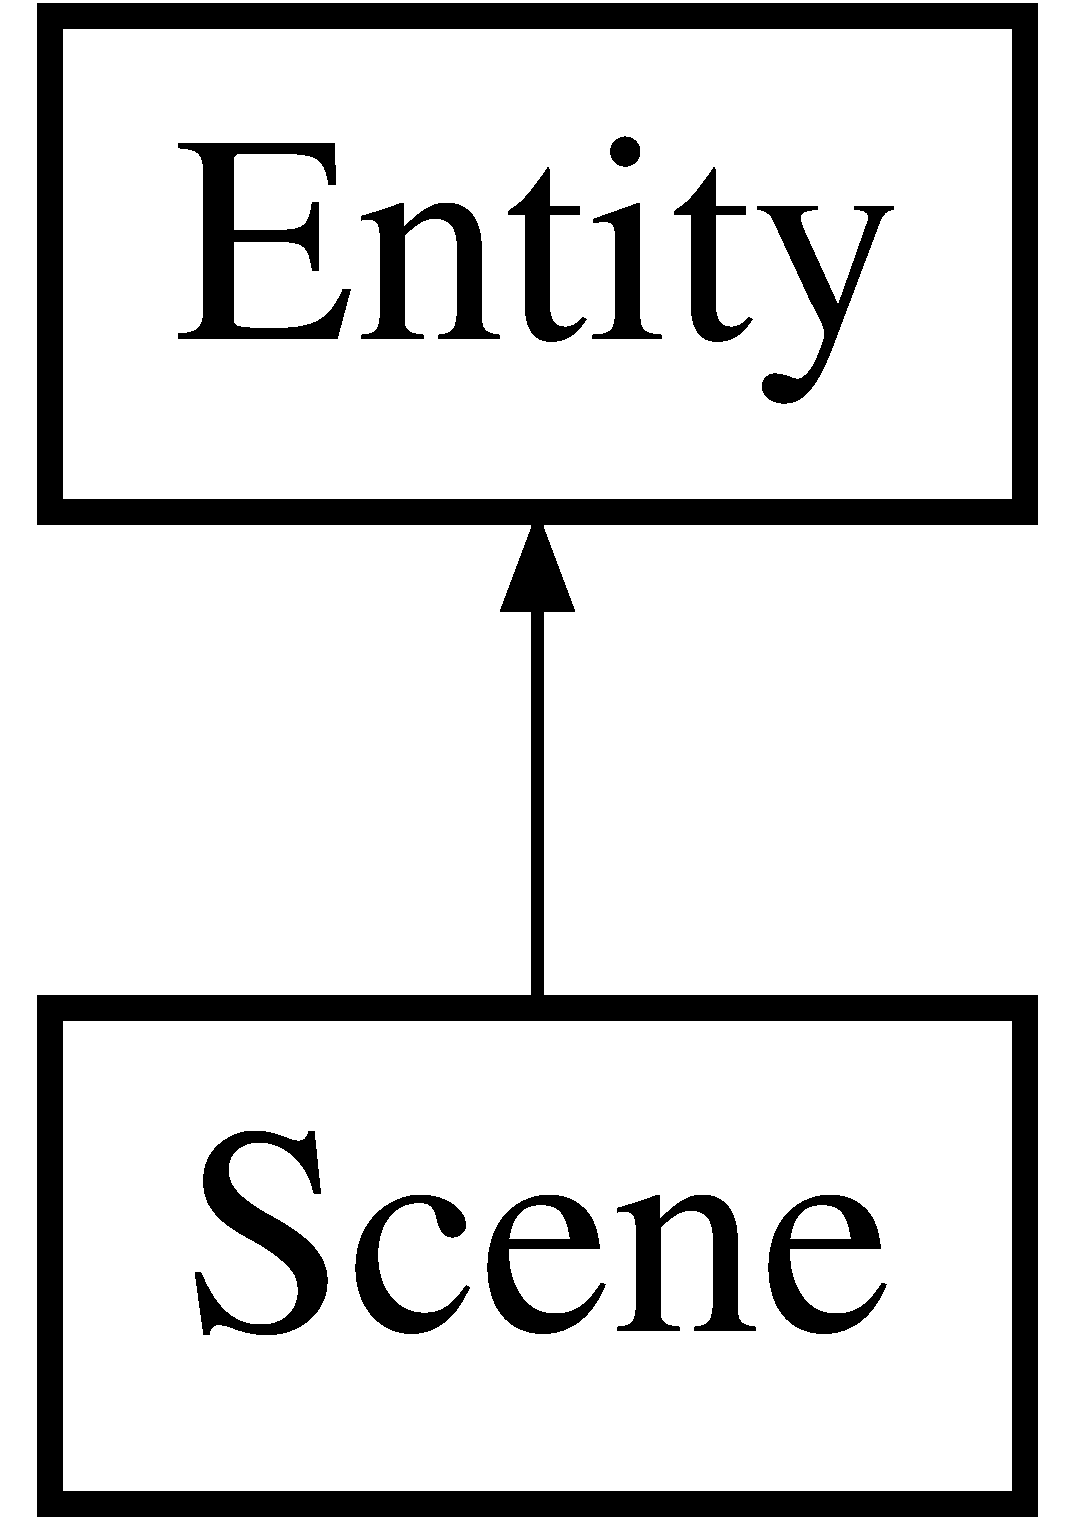
\includegraphics[height=2.000000cm]{class_scene}
\end{center}
\end{figure}
\subsection*{Public Member Functions}
\begin{DoxyCompactItemize}
\item 
\hyperlink{class_scene_ad10176d75a9cc0da56626f682d083507}{Scene} ()
\begin{DoxyCompactList}\small\item\em Constructor of the \hyperlink{class_scene}{Scene}. \end{DoxyCompactList}\item 
\mbox{\Hypertarget{class_scene_a3b8cec2e32546713915f8c6303c951f1}\label{class_scene_a3b8cec2e32546713915f8c6303c951f1}} 
virtual \hyperlink{class_scene_a3b8cec2e32546713915f8c6303c951f1}{$\sim$\+Scene} ()
\begin{DoxyCompactList}\small\item\em Destructor of the \hyperlink{class_scene}{Scene}. \end{DoxyCompactList}\item 
bool \hyperlink{class_scene_af6673f416884a66f46fd1e703d77de03}{is\+Running} ()
\begin{DoxyCompactList}\small\item\em whether this \hyperlink{class_scene}{Scene} is running or not. \end{DoxyCompactList}\item 
void \hyperlink{class_scene_af1c55c1cd88c6665609f5cba96dff226}{start} ()
\begin{DoxyCompactList}\small\item\em start running the \hyperlink{class_scene}{Scene} \end{DoxyCompactList}\item 
void \hyperlink{class_scene_add01794b17df2030e961468fc88cf2e7}{stop} ()
\begin{DoxyCompactList}\small\item\em stop running the \hyperlink{class_scene}{Scene} \end{DoxyCompactList}\item 
\hyperlink{class_camera}{Camera} $\ast$ \hyperlink{class_scene_a1845161fcd088622a1288a6c41bcd574}{camera} ()
\begin{DoxyCompactList}\small\item\em get a pointer to the \hyperlink{class_camera}{Camera} \end{DoxyCompactList}\item 
\hyperlink{class_input}{Input} $\ast$ \hyperlink{class_scene_ab8f8ccda2e6a954deb81d0f58c3b88bd}{input} ()
\begin{DoxyCompactList}\small\item\em get a pointer to the \hyperlink{class_input}{Input} \end{DoxyCompactList}\item 
void \hyperlink{class_scene_a7308b78f4cc3522369237623fd7a001f}{update\+Scene} (float delta\+Time)
\begin{DoxyCompactList}\small\item\em update this \hyperlink{class_scene}{Scene} \end{DoxyCompactList}\end{DoxyCompactItemize}
\subsection*{Additional Inherited Members}


\subsection{Detailed Description}
The \hyperlink{class_scene}{Scene} class is the Base class for your own Scenes. It has a \hyperlink{class_camera}{Camera}, \hyperlink{class_input}{Input} and basic on/off state machine. 

\subsection{Constructor \& Destructor Documentation}
\mbox{\Hypertarget{class_scene_ad10176d75a9cc0da56626f682d083507}\label{class_scene_ad10176d75a9cc0da56626f682d083507}} 
\index{Scene@{Scene}!Scene@{Scene}}
\index{Scene@{Scene}!Scene@{Scene}}
\subsubsection{\texorpdfstring{Scene()}{Scene()}}
{\footnotesize\ttfamily Scene\+::\+Scene (\begin{DoxyParamCaption}{ }\end{DoxyParamCaption})}



Constructor of the \hyperlink{class_scene}{Scene}. 

This file is part of R\+T2D, a 2D Open\+GL framework.


\begin{DoxyItemize}
\item Copyright 2015 Rik Teerling \href{mailto:rik@onandoffables.com}{\tt rik@onandoffables.\+com}
\begin{DoxyItemize}
\item Initial commit 
\end{DoxyItemize}
\end{DoxyItemize}

\subsection{Member Function Documentation}
\mbox{\Hypertarget{class_scene_a1845161fcd088622a1288a6c41bcd574}\label{class_scene_a1845161fcd088622a1288a6c41bcd574}} 
\index{Scene@{Scene}!camera@{camera}}
\index{camera@{camera}!Scene@{Scene}}
\subsubsection{\texorpdfstring{camera()}{camera()}}
{\footnotesize\ttfamily \hyperlink{class_camera}{Camera}$\ast$ Scene\+::camera (\begin{DoxyParamCaption}{ }\end{DoxyParamCaption})\hspace{0.3cm}{\ttfamily [inline]}}



get a pointer to the \hyperlink{class_camera}{Camera} 

\begin{DoxyReturn}{Returns}
Texture$\ast$ a pointer to the \hyperlink{class_camera}{Camera} 
\end{DoxyReturn}
\mbox{\Hypertarget{class_scene_ab8f8ccda2e6a954deb81d0f58c3b88bd}\label{class_scene_ab8f8ccda2e6a954deb81d0f58c3b88bd}} 
\index{Scene@{Scene}!input@{input}}
\index{input@{input}!Scene@{Scene}}
\subsubsection{\texorpdfstring{input()}{input()}}
{\footnotesize\ttfamily \hyperlink{class_input}{Input}$\ast$ Scene\+::input (\begin{DoxyParamCaption}{ }\end{DoxyParamCaption})\hspace{0.3cm}{\ttfamily [inline]}}



get a pointer to the \hyperlink{class_input}{Input} 

\begin{DoxyReturn}{Returns}
Input$\ast$ a pointer to the \hyperlink{class_input}{Input} 
\end{DoxyReturn}
\mbox{\Hypertarget{class_scene_af6673f416884a66f46fd1e703d77de03}\label{class_scene_af6673f416884a66f46fd1e703d77de03}} 
\index{Scene@{Scene}!is\+Running@{is\+Running}}
\index{is\+Running@{is\+Running}!Scene@{Scene}}
\subsubsection{\texorpdfstring{is\+Running()}{isRunning()}}
{\footnotesize\ttfamily bool Scene\+::is\+Running (\begin{DoxyParamCaption}{ }\end{DoxyParamCaption})\hspace{0.3cm}{\ttfamily [inline]}}



whether this \hyperlink{class_scene}{Scene} is running or not. 

\begin{DoxyReturn}{Returns}
bool \+\_\+is\+Running 
\end{DoxyReturn}
\mbox{\Hypertarget{class_scene_af1c55c1cd88c6665609f5cba96dff226}\label{class_scene_af1c55c1cd88c6665609f5cba96dff226}} 
\index{Scene@{Scene}!start@{start}}
\index{start@{start}!Scene@{Scene}}
\subsubsection{\texorpdfstring{start()}{start()}}
{\footnotesize\ttfamily void Scene\+::start (\begin{DoxyParamCaption}{ }\end{DoxyParamCaption})\hspace{0.3cm}{\ttfamily [inline]}}



start running the \hyperlink{class_scene}{Scene} 

\begin{DoxyReturn}{Returns}
void 
\end{DoxyReturn}
\mbox{\Hypertarget{class_scene_add01794b17df2030e961468fc88cf2e7}\label{class_scene_add01794b17df2030e961468fc88cf2e7}} 
\index{Scene@{Scene}!stop@{stop}}
\index{stop@{stop}!Scene@{Scene}}
\subsubsection{\texorpdfstring{stop()}{stop()}}
{\footnotesize\ttfamily void Scene\+::stop (\begin{DoxyParamCaption}{ }\end{DoxyParamCaption})\hspace{0.3cm}{\ttfamily [inline]}}



stop running the \hyperlink{class_scene}{Scene} 

\begin{DoxyReturn}{Returns}
void 
\end{DoxyReturn}
\mbox{\Hypertarget{class_scene_a7308b78f4cc3522369237623fd7a001f}\label{class_scene_a7308b78f4cc3522369237623fd7a001f}} 
\index{Scene@{Scene}!update\+Scene@{update\+Scene}}
\index{update\+Scene@{update\+Scene}!Scene@{Scene}}
\subsubsection{\texorpdfstring{update\+Scene()}{updateScene()}}
{\footnotesize\ttfamily void Scene\+::update\+Scene (\begin{DoxyParamCaption}\item[{float}]{delta\+Time }\end{DoxyParamCaption})}



update this \hyperlink{class_scene}{Scene} 


\begin{DoxyParams}{Parameters}
{\em delta\+Time} & the number of seconds since the last update \\
\hline
\end{DoxyParams}
\begin{DoxyReturn}{Returns}
void 
\end{DoxyReturn}


The documentation for this class was generated from the following files\+:\begin{DoxyCompactItemize}
\item 
\hyperlink{scene_8h}{scene.\+h}\item 
scene.\+cpp\end{DoxyCompactItemize}

\hypertarget{class_shader}{}\section{Shader Class Reference}
\label{class_shader}\index{Shader@{Shader}}


The \hyperlink{class_shader}{Shader} class loads vertex and fragment shader files, and compiles them into a \hyperlink{class_shader}{Shader}.  




{\ttfamily \#include $<$shader.\+h$>$}

\subsection*{Public Member Functions}
\begin{DoxyCompactItemize}
\item 
\mbox{\Hypertarget{class_shader_a0d654ebaca4e0555197c0724c6d30610}\label{class_shader_a0d654ebaca4e0555197c0724c6d30610}} 
\hyperlink{class_shader_a0d654ebaca4e0555197c0724c6d30610}{Shader} ()
\begin{DoxyCompactList}\small\item\em Constructor of the \hyperlink{class_shader}{Shader}. \end{DoxyCompactList}\item 
\mbox{\Hypertarget{class_shader_aff01df87e8a102f270b5b135a295e59d}\label{class_shader_aff01df87e8a102f270b5b135a295e59d}} 
virtual \hyperlink{class_shader_aff01df87e8a102f270b5b135a295e59d}{$\sim$\+Shader} ()
\begin{DoxyCompactList}\small\item\em Destructor of the \hyperlink{class_shader}{Shader}. \end{DoxyCompactList}\item 
G\+Luint \hyperlink{class_shader_a64691ffa0d0d8b5ecdc4d06e698422bd}{program\+ID} ()
\begin{DoxyCompactList}\small\item\em get the program\+ID \end{DoxyCompactList}\item 
G\+Luint \hyperlink{class_shader_ac9bb10cba974bc2fb4ba78758591967f}{matrix\+ID} ()
\begin{DoxyCompactList}\small\item\em get the Model\+View\+Projection Matrix\+ID \end{DoxyCompactList}\item 
G\+Luint \hyperlink{class_shader_abccab59f58d517c4c2ac392f522b0675}{texture\+ID} ()
\begin{DoxyCompactList}\small\item\em get the texture\+ID \end{DoxyCompactList}\item 
G\+Luint \hyperlink{class_shader_a3c7b58c01112d49cd433fa6479d54efb}{blend\+Color\+ID} ()
\begin{DoxyCompactList}\small\item\em get the blend\+Color\+ID \end{DoxyCompactList}\item 
G\+Luint \hyperlink{class_shader_af2060ae1c85d8db67389c8116a02d9dd}{uv\+Offset\+ID} ()
\begin{DoxyCompactList}\small\item\em get the uv\+Offset\+ID \end{DoxyCompactList}\item 
G\+Luint \hyperlink{class_shader_a7bc0245aea0f7c61d17a17273c2faaaf}{load\+Shaders} (const char $\ast$vertex\+\_\+file\+\_\+path, const char $\ast$fragment\+\_\+file\+\_\+path)
\begin{DoxyCompactList}\small\item\em load shaders from disk \end{DoxyCompactList}\end{DoxyCompactItemize}


\subsection{Detailed Description}
The \hyperlink{class_shader}{Shader} class loads vertex and fragment shader files, and compiles them into a \hyperlink{class_shader}{Shader}. 

\subsection{Member Function Documentation}
\mbox{\Hypertarget{class_shader_a3c7b58c01112d49cd433fa6479d54efb}\label{class_shader_a3c7b58c01112d49cd433fa6479d54efb}} 
\index{Shader@{Shader}!blend\+Color\+ID@{blend\+Color\+ID}}
\index{blend\+Color\+ID@{blend\+Color\+ID}!Shader@{Shader}}
\subsubsection{\texorpdfstring{blend\+Color\+I\+D()}{blendColorID()}}
{\footnotesize\ttfamily G\+Luint Shader\+::blend\+Color\+ID (\begin{DoxyParamCaption}{ }\end{DoxyParamCaption})\hspace{0.3cm}{\ttfamily [inline]}}



get the blend\+Color\+ID 

\begin{DoxyReturn}{Returns}
G\+Luint \+\_\+blend\+Color\+ID 
\end{DoxyReturn}
\mbox{\Hypertarget{class_shader_a7bc0245aea0f7c61d17a17273c2faaaf}\label{class_shader_a7bc0245aea0f7c61d17a17273c2faaaf}} 
\index{Shader@{Shader}!load\+Shaders@{load\+Shaders}}
\index{load\+Shaders@{load\+Shaders}!Shader@{Shader}}
\subsubsection{\texorpdfstring{load\+Shaders()}{loadShaders()}}
{\footnotesize\ttfamily G\+Luint Shader\+::load\+Shaders (\begin{DoxyParamCaption}\item[{const char $\ast$}]{vertex\+\_\+file\+\_\+path,  }\item[{const char $\ast$}]{fragment\+\_\+file\+\_\+path }\end{DoxyParamCaption})}



load shaders from disk 


\begin{DoxyParams}{Parameters}
{\em vertex\+\_\+file\+\_\+path} & path to vertexshader \\
\hline
{\em fragment\+\_\+file\+\_\+path} & path to fragmentshader \\
\hline
\end{DoxyParams}
\begin{DoxyReturn}{Returns}
G\+Luint \+\_\+program\+ID 
\end{DoxyReturn}
\mbox{\Hypertarget{class_shader_ac9bb10cba974bc2fb4ba78758591967f}\label{class_shader_ac9bb10cba974bc2fb4ba78758591967f}} 
\index{Shader@{Shader}!matrix\+ID@{matrix\+ID}}
\index{matrix\+ID@{matrix\+ID}!Shader@{Shader}}
\subsubsection{\texorpdfstring{matrix\+I\+D()}{matrixID()}}
{\footnotesize\ttfamily G\+Luint Shader\+::matrix\+ID (\begin{DoxyParamCaption}{ }\end{DoxyParamCaption})\hspace{0.3cm}{\ttfamily [inline]}}



get the Model\+View\+Projection Matrix\+ID 

\begin{DoxyReturn}{Returns}
G\+Luint \+\_\+matrix\+ID 
\end{DoxyReturn}
\mbox{\Hypertarget{class_shader_a64691ffa0d0d8b5ecdc4d06e698422bd}\label{class_shader_a64691ffa0d0d8b5ecdc4d06e698422bd}} 
\index{Shader@{Shader}!program\+ID@{program\+ID}}
\index{program\+ID@{program\+ID}!Shader@{Shader}}
\subsubsection{\texorpdfstring{program\+I\+D()}{programID()}}
{\footnotesize\ttfamily G\+Luint Shader\+::program\+ID (\begin{DoxyParamCaption}{ }\end{DoxyParamCaption})\hspace{0.3cm}{\ttfamily [inline]}}



get the program\+ID 

\begin{DoxyReturn}{Returns}
G\+Luint \+\_\+program\+ID 
\end{DoxyReturn}
\mbox{\Hypertarget{class_shader_abccab59f58d517c4c2ac392f522b0675}\label{class_shader_abccab59f58d517c4c2ac392f522b0675}} 
\index{Shader@{Shader}!texture\+ID@{texture\+ID}}
\index{texture\+ID@{texture\+ID}!Shader@{Shader}}
\subsubsection{\texorpdfstring{texture\+I\+D()}{textureID()}}
{\footnotesize\ttfamily G\+Luint Shader\+::texture\+ID (\begin{DoxyParamCaption}{ }\end{DoxyParamCaption})\hspace{0.3cm}{\ttfamily [inline]}}



get the texture\+ID 

\begin{DoxyReturn}{Returns}
G\+Luint \+\_\+texture\+ID 
\end{DoxyReturn}
\mbox{\Hypertarget{class_shader_af2060ae1c85d8db67389c8116a02d9dd}\label{class_shader_af2060ae1c85d8db67389c8116a02d9dd}} 
\index{Shader@{Shader}!uv\+Offset\+ID@{uv\+Offset\+ID}}
\index{uv\+Offset\+ID@{uv\+Offset\+ID}!Shader@{Shader}}
\subsubsection{\texorpdfstring{uv\+Offset\+I\+D()}{uvOffsetID()}}
{\footnotesize\ttfamily G\+Luint Shader\+::uv\+Offset\+ID (\begin{DoxyParamCaption}{ }\end{DoxyParamCaption})\hspace{0.3cm}{\ttfamily [inline]}}



get the uv\+Offset\+ID 

\begin{DoxyReturn}{Returns}
G\+Luint \+\_\+uv\+Offset\+ID 
\end{DoxyReturn}


The documentation for this class was generated from the following files\+:\begin{DoxyCompactItemize}
\item 
\hyperlink{shader_8h}{shader.\+h}\item 
shader.\+cpp\end{DoxyCompactItemize}

\hypertarget{class_sprite}{}\section{Sprite Class Reference}
\label{class_sprite}\index{Sprite@{Sprite}}


The \hyperlink{class_sprite}{Sprite} class defines the \hyperlink{class_texture}{Texture}, \hyperlink{class_shader}{Shader}, blend \hyperlink{struct_color}{Color} and pivot point of a \hyperlink{class_sprite}{Sprite}.  




{\ttfamily \#include $<$sprite.\+h$>$}

\subsection*{Public Member Functions}
\begin{DoxyCompactItemize}
\item 
\hyperlink{class_sprite_a12cba3ac1868418add3c4d95ce87e615}{Sprite} ()
\begin{DoxyCompactList}\small\item\em Constructor of the \hyperlink{class_sprite}{Sprite}. \end{DoxyCompactList}\item 
\mbox{\Hypertarget{class_sprite_a8accab430f9d90ae5117b57d67e32b84}\label{class_sprite_a8accab430f9d90ae5117b57d67e32b84}} 
virtual \hyperlink{class_sprite_a8accab430f9d90ae5117b57d67e32b84}{$\sim$\+Sprite} ()
\begin{DoxyCompactList}\small\item\em Destructor of the \hyperlink{class_sprite}{Sprite}. \end{DoxyCompactList}\item 
std\+::string \hyperlink{class_sprite_aa82471010f1e9e5fb6e641d3f4601965}{texturename} ()
\begin{DoxyCompactList}\small\item\em get the texturename (path to the file) \end{DoxyCompactList}\item 
void \hyperlink{class_sprite_a53c2368c7940851a59a4717c0909e828}{texturename} (std\+::string texturename)
\begin{DoxyCompactList}\small\item\em set the texturename (path to the file) \end{DoxyCompactList}\item 
std\+::string \hyperlink{class_sprite_a62f75a2c234025b6cfc6525bd4ae1da8}{fragmentshader} ()
\begin{DoxyCompactList}\small\item\em get the fragmentshader (path to the file) \end{DoxyCompactList}\item 
std\+::string \hyperlink{class_sprite_aae341238d43e34f9e479355f72902cda}{vertexshader} ()
\begin{DoxyCompactList}\small\item\em get the vertexshader (path to the file) \end{DoxyCompactList}\item 
void \hyperlink{class_sprite_a7934a50c082a996333a02d5d8196cfa3}{fragmentshader} (std\+::string fragmentshader)
\begin{DoxyCompactList}\small\item\em set the fragmentshader (path to the file) \end{DoxyCompactList}\item 
void \hyperlink{class_sprite_ac5271cb1c478761a433969f03699894c}{vertexshader} (std\+::string vertexshader)
\begin{DoxyCompactList}\small\item\em set the vertexshader (path to the file) \end{DoxyCompactList}\item 
int \hyperlink{class_sprite_a150a85459279f9ef94eac9376736cab0}{frame} (int f)
\begin{DoxyCompactList}\small\item\em set the current frame \end{DoxyCompactList}\item 
int \hyperlink{class_sprite_a59437773b51f5c9abba5c8dabd2fbdb4}{frame} ()
\begin{DoxyCompactList}\small\item\em get the current frame \end{DoxyCompactList}\item 
void \hyperlink{class_sprite_afd130a4d3383e9d9c53048e282e3fb27}{setup\+Sprite} (const std\+::string \&filename, float pivotx, float pivoty, float uvwidth, float uvheight)
\begin{DoxyCompactList}\small\item\em prepare \hyperlink{class_sprite}{Sprite} for creation by \hyperlink{class_resource_manager}{Resource\+Manager} \end{DoxyCompactList}\item 
void \hyperlink{class_sprite_a4fb77e0618b77634c172edbc203549d3}{setup\+Circle\+Sprite} (const std\+::string \&filename, int radius, int segments)
\begin{DoxyCompactList}\small\item\em prepare Circle \hyperlink{class_sprite}{Sprite} for creation by \hyperlink{class_resource_manager}{Resource\+Manager} \end{DoxyCompactList}\item 
void \hyperlink{class_sprite_a9221cee6ad17032a77edb060cbca8ae7}{setup\+Segment\+Sprite} (const std\+::string \&filename, int radius, int segments, int \hyperlink{class_sprite_a0bfc3bb83da3bef06696cb55b5c47465}{which})
\begin{DoxyCompactList}\small\item\em prepare Circle \hyperlink{class_sprite}{Sprite} for creation by \hyperlink{class_resource_manager}{Resource\+Manager} \end{DoxyCompactList}\item 
void \hyperlink{class_sprite_a9d55a71e8a3d02936392535fece67c31}{setup\+Sprite} (const std\+::string \&filename, float pivotx, float pivoty, float uvwidth, float uvheight, int \hyperlink{class_sprite_a02160c2a56ce86d59b827899bab9c5b5}{filter}, int \hyperlink{class_sprite_a0e10957a274ba27a38601eac1fda210c}{wrap})
\begin{DoxyCompactList}\small\item\em prepare \hyperlink{class_sprite}{Sprite} for creation by \hyperlink{class_resource_manager}{Resource\+Manager} \end{DoxyCompactList}\item 
void \hyperlink{class_sprite_ad0f4f4d9337f5da714183d4eaec29d42}{setup\+Sprite\+By\+Pixel\+Buffer} (\hyperlink{struct_pixel_buffer}{Pixel\+Buffer} $\ast$pixels)
\begin{DoxyCompactList}\small\item\em Fill the \hyperlink{struct_pixel_buffer}{Pixel\+Buffer} of this \hyperlink{class_sprite}{Sprite}. \end{DoxyCompactList}\item 
void \hyperlink{class_sprite_a7f713b5e91889cba8202ffc91b60be84}{setup\+Sprite\+T\+G\+A\+Pixel\+Buffer} (const std\+::string \&filename, int \hyperlink{class_sprite_a02160c2a56ce86d59b827899bab9c5b5}{filter}, int \hyperlink{class_sprite_a0e10957a274ba27a38601eac1fda210c}{wrap})
\begin{DoxyCompactList}\small\item\em Fill the \hyperlink{struct_pixel_buffer}{Pixel\+Buffer} of this \hyperlink{class_sprite}{Sprite} with pixels from a file. \end{DoxyCompactList}\item 
\hyperlink{class_texture}{Texture} $\ast$ \hyperlink{class_sprite_a455494cddd7e1b8397f1c48cb5d461ec}{texture} ()
\begin{DoxyCompactList}\small\item\em get the dynamic texture \end{DoxyCompactList}\item 
bool \hyperlink{class_sprite_addbab8d45f865a551c5e012a4f63b8b7}{dynamic} ()
\begin{DoxyCompactList}\small\item\em is this \hyperlink{class_line}{Line} dynamic or not? \end{DoxyCompactList}\item 
void \hyperlink{class_sprite_a8164c86f45c115f8b45ddf2dc72f7be8}{dynamic} (bool d)
\begin{DoxyCompactList}\small\item\em set this \hyperlink{class_line}{Line} to be dynamic or not \end{DoxyCompactList}\item 
void \hyperlink{class_sprite_a02160c2a56ce86d59b827899bab9c5b5}{filter} (int f)
\begin{DoxyCompactList}\small\item\em set filter for this \hyperlink{class_sprite}{Sprite} \end{DoxyCompactList}\item 
int \hyperlink{class_sprite_a7c183f627af8bf9d416189f4dc81383b}{filter} ()
\begin{DoxyCompactList}\small\item\em get filter for this \hyperlink{class_sprite}{Sprite} \end{DoxyCompactList}\item 
void \hyperlink{class_sprite_a0e10957a274ba27a38601eac1fda210c}{wrap} (int w)
\begin{DoxyCompactList}\small\item\em set wrap for this \hyperlink{class_sprite}{Sprite} \end{DoxyCompactList}\item 
int \hyperlink{class_sprite_a5b8eb7dc4c186c951ebf1b424cdda27f}{wrap} ()
\begin{DoxyCompactList}\small\item\em get wrap for this \hyperlink{class_sprite}{Sprite} \end{DoxyCompactList}\item 
int \hyperlink{class_sprite_a0bfc3bb83da3bef06696cb55b5c47465}{which} ()
\begin{DoxyCompactList}\small\item\em get which segment of circle this sprite has. \end{DoxyCompactList}\item 
int \hyperlink{class_sprite_ad7827d61c0d5f95499df3bcc569cd33c}{circlemesh} ()
\begin{DoxyCompactList}\small\item\em get if this is a circlemesh or not. \end{DoxyCompactList}\item 
int \hyperlink{class_sprite_af008075858671c5cfad4fe679b93273b}{use\+Culling} ()
\begin{DoxyCompactList}\small\item\em check if this \hyperlink{class_sprite}{Sprite} uses culling \end{DoxyCompactList}\item 
void \hyperlink{class_sprite_acf75b5a4882d1cb20a77244feeb0d2f3}{use\+Culling} (int c)
\begin{DoxyCompactList}\small\item\em use culling on this \hyperlink{class_sprite}{Sprite} or not \end{DoxyCompactList}\end{DoxyCompactItemize}
\subsection*{Public Attributes}
\begin{DoxyCompactItemize}
\item 
\mbox{\Hypertarget{class_sprite_a7f76c78f2f69d6cc0689bee7fbc2d57f}\label{class_sprite_a7f76c78f2f69d6cc0689bee7fbc2d57f}} 
\hyperlink{pointx_8h_aca903a92c8ced8823fea9fac7e23677a}{Point2} \hyperlink{class_sprite_a7f76c78f2f69d6cc0689bee7fbc2d57f}{spriteposition}
\begin{DoxyCompactList}\small\item\em \hyperlink{class_sprite}{Sprite} position \hyperlink{class_point__t}{Point\+\_\+t} of the \hyperlink{class_sprite}{Sprite} (only for Spritebatches) \end{DoxyCompactList}\item 
\mbox{\Hypertarget{class_sprite_a6a28de683885ecffa2c5934cd0df330b}\label{class_sprite_a6a28de683885ecffa2c5934cd0df330b}} 
float \hyperlink{class_sprite_a6a28de683885ecffa2c5934cd0df330b}{spriterotation}
\begin{DoxyCompactList}\small\item\em \hyperlink{class_sprite}{Sprite} rotation of the \hyperlink{class_sprite}{Sprite} (only for Spritebatches) \end{DoxyCompactList}\item 
\mbox{\Hypertarget{class_sprite_a458d2b177ceb0b0ba4030b47d4e4cb39}\label{class_sprite_a458d2b177ceb0b0ba4030b47d4e4cb39}} 
\hyperlink{pointx_8h_aca903a92c8ced8823fea9fac7e23677a}{Point2} \hyperlink{class_sprite_a458d2b177ceb0b0ba4030b47d4e4cb39}{spritescale}
\begin{DoxyCompactList}\small\item\em \hyperlink{class_sprite}{Sprite} scale \hyperlink{class_point__t}{Point\+\_\+t} of the \hyperlink{class_sprite}{Sprite} (only for Spritebatches) \end{DoxyCompactList}\item 
\mbox{\Hypertarget{class_sprite_a8378b1b658e1fa4b364b499f7b52b820}\label{class_sprite_a8378b1b658e1fa4b364b499f7b52b820}} 
\hyperlink{pointx_8h_aca903a92c8ced8823fea9fac7e23677a}{Point2} \hyperlink{class_sprite_a8378b1b658e1fa4b364b499f7b52b820}{pivot}
\begin{DoxyCompactList}\small\item\em Pivot \hyperlink{class_point__t}{Point\+\_\+t} of the \hyperlink{class_sprite}{Sprite}. \end{DoxyCompactList}\item 
\mbox{\Hypertarget{class_sprite_af01ad3049736a7ff720a86b35c93a6bb}\label{class_sprite_af01ad3049736a7ff720a86b35c93a6bb}} 
\hyperlink{pointx_8h_aca903a92c8ced8823fea9fac7e23677a}{Point2} \hyperlink{class_sprite_af01ad3049736a7ff720a86b35c93a6bb}{uvdim}
\begin{DoxyCompactList}\small\item\em U\+Vdim \hyperlink{class_point__t}{Point\+\_\+t} of the \hyperlink{class_sprite}{Sprite} (uvwidth, uvheight. The size of the part we need to render) \end{DoxyCompactList}\item 
\mbox{\Hypertarget{class_sprite_a6d546e83a70f018bb300c3e1d7202252}\label{class_sprite_a6d546e83a70f018bb300c3e1d7202252}} 
\hyperlink{pointx_8h_aca903a92c8ced8823fea9fac7e23677a}{Point2} \hyperlink{class_sprite_a6d546e83a70f018bb300c3e1d7202252}{uvoffset}
\begin{DoxyCompactList}\small\item\em U\+Voffset \hyperlink{class_point__t}{Point\+\_\+t} of the \hyperlink{class_sprite}{Sprite} (which part do we need to render) \end{DoxyCompactList}\item 
\mbox{\Hypertarget{class_sprite_ab1eced6c668a22855d4817fddd6d83b0}\label{class_sprite_ab1eced6c668a22855d4817fddd6d83b0}} 
\hyperlink{pointx_8h_aca903a92c8ced8823fea9fac7e23677a}{Point2} \hyperlink{class_sprite_ab1eced6c668a22855d4817fddd6d83b0}{size}
\begin{DoxyCompactList}\small\item\em size \hyperlink{class_point__t}{Point\+\_\+t} of the \hyperlink{class_sprite}{Sprite} (width and height of the \hyperlink{class_sprite}{Sprite}) \end{DoxyCompactList}\item 
\mbox{\Hypertarget{class_sprite_a5604ec44c78749153a4fa6d37cab3af0}\label{class_sprite_a5604ec44c78749153a4fa6d37cab3af0}} 
\hyperlink{struct_r_g_b_a_color}{R\+G\+B\+A\+Color} \hyperlink{class_sprite_a5604ec44c78749153a4fa6d37cab3af0}{color}
\begin{DoxyCompactList}\small\item\em blend \hyperlink{struct_color}{Color} of the \hyperlink{class_sprite}{Sprite} \end{DoxyCompactList}\end{DoxyCompactItemize}


\subsection{Detailed Description}
The \hyperlink{class_sprite}{Sprite} class defines the \hyperlink{class_texture}{Texture}, \hyperlink{class_shader}{Shader}, blend \hyperlink{struct_color}{Color} and pivot point of a \hyperlink{class_sprite}{Sprite}. 

\subsection{Constructor \& Destructor Documentation}
\mbox{\Hypertarget{class_sprite_a12cba3ac1868418add3c4d95ce87e615}\label{class_sprite_a12cba3ac1868418add3c4d95ce87e615}} 
\index{Sprite@{Sprite}!Sprite@{Sprite}}
\index{Sprite@{Sprite}!Sprite@{Sprite}}
\subsubsection{\texorpdfstring{Sprite()}{Sprite()}}
{\footnotesize\ttfamily Sprite\+::\+Sprite (\begin{DoxyParamCaption}{ }\end{DoxyParamCaption})}



Constructor of the \hyperlink{class_sprite}{Sprite}. 

This file is part of R\+T2D, a 2D Open\+GL framework.


\begin{DoxyItemize}
\item Copyright 2015 Rik Teerling \href{mailto:rik@onandoffables.com}{\tt rik@onandoffables.\+com}
\begin{DoxyItemize}
\item Initial commit 
\end{DoxyItemize}
\end{DoxyItemize}

\subsection{Member Function Documentation}
\mbox{\Hypertarget{class_sprite_ad7827d61c0d5f95499df3bcc569cd33c}\label{class_sprite_ad7827d61c0d5f95499df3bcc569cd33c}} 
\index{Sprite@{Sprite}!circlemesh@{circlemesh}}
\index{circlemesh@{circlemesh}!Sprite@{Sprite}}
\subsubsection{\texorpdfstring{circlemesh()}{circlemesh()}}
{\footnotesize\ttfamily int Sprite\+::circlemesh (\begin{DoxyParamCaption}{ }\end{DoxyParamCaption})\hspace{0.3cm}{\ttfamily [inline]}}



get if this is a circlemesh or not. 

0 = no circlemesh n = amounts of total segments in the circle (6 for hexagon) \begin{DoxyReturn}{Returns}
int \+\_\+circlemesh 
\end{DoxyReturn}
\mbox{\Hypertarget{class_sprite_addbab8d45f865a551c5e012a4f63b8b7}\label{class_sprite_addbab8d45f865a551c5e012a4f63b8b7}} 
\index{Sprite@{Sprite}!dynamic@{dynamic}}
\index{dynamic@{dynamic}!Sprite@{Sprite}}
\subsubsection{\texorpdfstring{dynamic()}{dynamic()}\hspace{0.1cm}{\footnotesize\ttfamily [1/2]}}
{\footnotesize\ttfamily bool Sprite\+::dynamic (\begin{DoxyParamCaption}{ }\end{DoxyParamCaption})\hspace{0.3cm}{\ttfamily [inline]}}



is this \hyperlink{class_line}{Line} dynamic or not? 

\begin{DoxyReturn}{Returns}
bool \+\_\+dynamic 
\end{DoxyReturn}
\mbox{\Hypertarget{class_sprite_a8164c86f45c115f8b45ddf2dc72f7be8}\label{class_sprite_a8164c86f45c115f8b45ddf2dc72f7be8}} 
\index{Sprite@{Sprite}!dynamic@{dynamic}}
\index{dynamic@{dynamic}!Sprite@{Sprite}}
\subsubsection{\texorpdfstring{dynamic()}{dynamic()}\hspace{0.1cm}{\footnotesize\ttfamily [2/2]}}
{\footnotesize\ttfamily void Sprite\+::dynamic (\begin{DoxyParamCaption}\item[{bool}]{d }\end{DoxyParamCaption})\hspace{0.3cm}{\ttfamily [inline]}}



set this \hyperlink{class_line}{Line} to be dynamic or not 

\begin{DoxyReturn}{Returns}
void 
\end{DoxyReturn}
\mbox{\Hypertarget{class_sprite_a02160c2a56ce86d59b827899bab9c5b5}\label{class_sprite_a02160c2a56ce86d59b827899bab9c5b5}} 
\index{Sprite@{Sprite}!filter@{filter}}
\index{filter@{filter}!Sprite@{Sprite}}
\subsubsection{\texorpdfstring{filter()}{filter()}\hspace{0.1cm}{\footnotesize\ttfamily [1/2]}}
{\footnotesize\ttfamily void Sprite\+::filter (\begin{DoxyParamCaption}\item[{int}]{f }\end{DoxyParamCaption})\hspace{0.3cm}{\ttfamily [inline]}}



set filter for this \hyperlink{class_sprite}{Sprite} 

\begin{DoxyReturn}{Returns}
void 
\end{DoxyReturn}
\mbox{\Hypertarget{class_sprite_a7c183f627af8bf9d416189f4dc81383b}\label{class_sprite_a7c183f627af8bf9d416189f4dc81383b}} 
\index{Sprite@{Sprite}!filter@{filter}}
\index{filter@{filter}!Sprite@{Sprite}}
\subsubsection{\texorpdfstring{filter()}{filter()}\hspace{0.1cm}{\footnotesize\ttfamily [2/2]}}
{\footnotesize\ttfamily int Sprite\+::filter (\begin{DoxyParamCaption}{ }\end{DoxyParamCaption})\hspace{0.3cm}{\ttfamily [inline]}}



get filter for this \hyperlink{class_sprite}{Sprite} 

\begin{DoxyReturn}{Returns}
int \+\_\+filter 
\end{DoxyReturn}
\mbox{\Hypertarget{class_sprite_a62f75a2c234025b6cfc6525bd4ae1da8}\label{class_sprite_a62f75a2c234025b6cfc6525bd4ae1da8}} 
\index{Sprite@{Sprite}!fragmentshader@{fragmentshader}}
\index{fragmentshader@{fragmentshader}!Sprite@{Sprite}}
\subsubsection{\texorpdfstring{fragmentshader()}{fragmentshader()}\hspace{0.1cm}{\footnotesize\ttfamily [1/2]}}
{\footnotesize\ttfamily std\+::string Sprite\+::fragmentshader (\begin{DoxyParamCaption}{ }\end{DoxyParamCaption})\hspace{0.3cm}{\ttfamily [inline]}}



get the fragmentshader (path to the file) 

\begin{DoxyReturn}{Returns}
std\+::string \+\_\+fragmentshader 
\end{DoxyReturn}
\mbox{\Hypertarget{class_sprite_a7934a50c082a996333a02d5d8196cfa3}\label{class_sprite_a7934a50c082a996333a02d5d8196cfa3}} 
\index{Sprite@{Sprite}!fragmentshader@{fragmentshader}}
\index{fragmentshader@{fragmentshader}!Sprite@{Sprite}}
\subsubsection{\texorpdfstring{fragmentshader()}{fragmentshader()}\hspace{0.1cm}{\footnotesize\ttfamily [2/2]}}
{\footnotesize\ttfamily void Sprite\+::fragmentshader (\begin{DoxyParamCaption}\item[{std\+::string}]{fragmentshader }\end{DoxyParamCaption})\hspace{0.3cm}{\ttfamily [inline]}}



set the fragmentshader (path to the file) 


\begin{DoxyParams}{Parameters}
{\em fragmentshader} & path to fragmentshader \\
\hline
\end{DoxyParams}
\begin{DoxyReturn}{Returns}
void 
\end{DoxyReturn}
\mbox{\Hypertarget{class_sprite_a150a85459279f9ef94eac9376736cab0}\label{class_sprite_a150a85459279f9ef94eac9376736cab0}} 
\index{Sprite@{Sprite}!frame@{frame}}
\index{frame@{frame}!Sprite@{Sprite}}
\subsubsection{\texorpdfstring{frame()}{frame()}\hspace{0.1cm}{\footnotesize\ttfamily [1/2]}}
{\footnotesize\ttfamily int Sprite\+::frame (\begin{DoxyParamCaption}\item[{int}]{f }\end{DoxyParamCaption})}



set the current frame 

\begin{DoxyReturn}{Returns}
int \+\_\+frame 
\end{DoxyReturn}
\mbox{\Hypertarget{class_sprite_a59437773b51f5c9abba5c8dabd2fbdb4}\label{class_sprite_a59437773b51f5c9abba5c8dabd2fbdb4}} 
\index{Sprite@{Sprite}!frame@{frame}}
\index{frame@{frame}!Sprite@{Sprite}}
\subsubsection{\texorpdfstring{frame()}{frame()}\hspace{0.1cm}{\footnotesize\ttfamily [2/2]}}
{\footnotesize\ttfamily int Sprite\+::frame (\begin{DoxyParamCaption}{ }\end{DoxyParamCaption})\hspace{0.3cm}{\ttfamily [inline]}}



get the current frame 

\begin{DoxyReturn}{Returns}
int \+\_\+frame 
\end{DoxyReturn}
\mbox{\Hypertarget{class_sprite_a4fb77e0618b77634c172edbc203549d3}\label{class_sprite_a4fb77e0618b77634c172edbc203549d3}} 
\index{Sprite@{Sprite}!setup\+Circle\+Sprite@{setup\+Circle\+Sprite}}
\index{setup\+Circle\+Sprite@{setup\+Circle\+Sprite}!Sprite@{Sprite}}
\subsubsection{\texorpdfstring{setup\+Circle\+Sprite()}{setupCircleSprite()}}
{\footnotesize\ttfamily void Sprite\+::setup\+Circle\+Sprite (\begin{DoxyParamCaption}\item[{const std\+::string \&}]{filename,  }\item[{int}]{radius,  }\item[{int}]{segments }\end{DoxyParamCaption})}



prepare Circle \hyperlink{class_sprite}{Sprite} for creation by \hyperlink{class_resource_manager}{Resource\+Manager} 


\begin{DoxyParams}{Parameters}
{\em filename} & path to the image.\+tga \\
\hline
{\em radius} & of the circle \\
\hline
{\em segments} & of the circle \\
\hline
\end{DoxyParams}
\begin{DoxyReturn}{Returns}
void 
\end{DoxyReturn}
\mbox{\Hypertarget{class_sprite_a9221cee6ad17032a77edb060cbca8ae7}\label{class_sprite_a9221cee6ad17032a77edb060cbca8ae7}} 
\index{Sprite@{Sprite}!setup\+Segment\+Sprite@{setup\+Segment\+Sprite}}
\index{setup\+Segment\+Sprite@{setup\+Segment\+Sprite}!Sprite@{Sprite}}
\subsubsection{\texorpdfstring{setup\+Segment\+Sprite()}{setupSegmentSprite()}}
{\footnotesize\ttfamily void Sprite\+::setup\+Segment\+Sprite (\begin{DoxyParamCaption}\item[{const std\+::string \&}]{filename,  }\item[{int}]{radius,  }\item[{int}]{segments,  }\item[{int}]{which }\end{DoxyParamCaption})}



prepare Circle \hyperlink{class_sprite}{Sprite} for creation by \hyperlink{class_resource_manager}{Resource\+Manager} 


\begin{DoxyParams}{Parameters}
{\em filename} & path to the image.\+tga \\
\hline
{\em radius} & of the circle \\
\hline
{\em segments} & of the circle \\
\hline
{\em which} & which part of the circle \\
\hline
\end{DoxyParams}
\begin{DoxyReturn}{Returns}
void 
\end{DoxyReturn}
\mbox{\Hypertarget{class_sprite_afd130a4d3383e9d9c53048e282e3fb27}\label{class_sprite_afd130a4d3383e9d9c53048e282e3fb27}} 
\index{Sprite@{Sprite}!setup\+Sprite@{setup\+Sprite}}
\index{setup\+Sprite@{setup\+Sprite}!Sprite@{Sprite}}
\subsubsection{\texorpdfstring{setup\+Sprite()}{setupSprite()}\hspace{0.1cm}{\footnotesize\ttfamily [1/2]}}
{\footnotesize\ttfamily void Sprite\+::setup\+Sprite (\begin{DoxyParamCaption}\item[{const std\+::string \&}]{filename,  }\item[{float}]{pivotx,  }\item[{float}]{pivoty,  }\item[{float}]{uvwidth,  }\item[{float}]{uvheight }\end{DoxyParamCaption})}



prepare \hyperlink{class_sprite}{Sprite} for creation by \hyperlink{class_resource_manager}{Resource\+Manager} 


\begin{DoxyParams}{Parameters}
{\em filename} & path to the image.\+tga \\
\hline
{\em pivotx} & X component of Pivot \hyperlink{class_point__t}{Point\+\_\+t} of the \hyperlink{class_sprite}{Sprite} \\
\hline
{\em pivoty} & Y component of Pivot \hyperlink{class_point__t}{Point\+\_\+t} of the \hyperlink{class_sprite}{Sprite} \\
\hline
{\em uvwidth} & 1.\+0f=full texture, 0.\+5f=2x2 texture, 0.\+25f=4x4 texture etc. \\
\hline
{\em uvheight} & 1.\+0f=full texture, 0.\+5f=2x2 texture, 0.\+25f=4x4 texture etc. \\
\hline
\end{DoxyParams}
\begin{DoxyReturn}{Returns}
void 
\end{DoxyReturn}
\mbox{\Hypertarget{class_sprite_a9d55a71e8a3d02936392535fece67c31}\label{class_sprite_a9d55a71e8a3d02936392535fece67c31}} 
\index{Sprite@{Sprite}!setup\+Sprite@{setup\+Sprite}}
\index{setup\+Sprite@{setup\+Sprite}!Sprite@{Sprite}}
\subsubsection{\texorpdfstring{setup\+Sprite()}{setupSprite()}\hspace{0.1cm}{\footnotesize\ttfamily [2/2]}}
{\footnotesize\ttfamily void Sprite\+::setup\+Sprite (\begin{DoxyParamCaption}\item[{const std\+::string \&}]{filename,  }\item[{float}]{pivotx,  }\item[{float}]{pivoty,  }\item[{float}]{uvwidth,  }\item[{float}]{uvheight,  }\item[{int}]{filter,  }\item[{int}]{wrap }\end{DoxyParamCaption})}



prepare \hyperlink{class_sprite}{Sprite} for creation by \hyperlink{class_resource_manager}{Resource\+Manager} 


\begin{DoxyParams}{Parameters}
{\em filename} & path to the image.\+tga \\
\hline
{\em pivotx} & X component of Pivot \hyperlink{class_point__t}{Point\+\_\+t} of the \hyperlink{class_sprite}{Sprite} \\
\hline
{\em pivoty} & Y component of Pivot \hyperlink{class_point__t}{Point\+\_\+t} of the \hyperlink{class_sprite}{Sprite} \\
\hline
{\em uvwidth} & 1.\+0f=full texture, 0.\+5f=2x2 texture, 0.\+25f=4x4 texture etc. \\
\hline
{\em uvheight} & 1.\+0f=full texture, 0.\+5f=2x2 texture, 0.\+25f=4x4 texture etc. \\
\hline
{\em filter} & filter of the \hyperlink{class_sprite}{Sprite} \hyperlink{class_texture}{Texture} \\
\hline
{\em wrap} & wrapping of the \hyperlink{class_sprite}{Sprite} \hyperlink{class_texture}{Texture} \\
\hline
\end{DoxyParams}
\begin{DoxyReturn}{Returns}
void 
\end{DoxyReturn}
\mbox{\Hypertarget{class_sprite_ad0f4f4d9337f5da714183d4eaec29d42}\label{class_sprite_ad0f4f4d9337f5da714183d4eaec29d42}} 
\index{Sprite@{Sprite}!setup\+Sprite\+By\+Pixel\+Buffer@{setup\+Sprite\+By\+Pixel\+Buffer}}
\index{setup\+Sprite\+By\+Pixel\+Buffer@{setup\+Sprite\+By\+Pixel\+Buffer}!Sprite@{Sprite}}
\subsubsection{\texorpdfstring{setup\+Sprite\+By\+Pixel\+Buffer()}{setupSpriteByPixelBuffer()}}
{\footnotesize\ttfamily void Sprite\+::setup\+Sprite\+By\+Pixel\+Buffer (\begin{DoxyParamCaption}\item[{\hyperlink{struct_pixel_buffer}{Pixel\+Buffer} $\ast$}]{pixels }\end{DoxyParamCaption})}



Fill the \hyperlink{struct_pixel_buffer}{Pixel\+Buffer} of this \hyperlink{class_sprite}{Sprite}. 


\begin{DoxyParams}{Parameters}
{\em pixels} & a \hyperlink{struct_pixel_buffer}{Pixel\+Buffer} pointer \\
\hline
\end{DoxyParams}
\begin{DoxyReturn}{Returns}
void 
\end{DoxyReturn}
\mbox{\Hypertarget{class_sprite_a7f713b5e91889cba8202ffc91b60be84}\label{class_sprite_a7f713b5e91889cba8202ffc91b60be84}} 
\index{Sprite@{Sprite}!setup\+Sprite\+T\+G\+A\+Pixel\+Buffer@{setup\+Sprite\+T\+G\+A\+Pixel\+Buffer}}
\index{setup\+Sprite\+T\+G\+A\+Pixel\+Buffer@{setup\+Sprite\+T\+G\+A\+Pixel\+Buffer}!Sprite@{Sprite}}
\subsubsection{\texorpdfstring{setup\+Sprite\+T\+G\+A\+Pixel\+Buffer()}{setupSpriteTGAPixelBuffer()}}
{\footnotesize\ttfamily void Sprite\+::setup\+Sprite\+T\+G\+A\+Pixel\+Buffer (\begin{DoxyParamCaption}\item[{const std\+::string \&}]{filename,  }\item[{int}]{filter,  }\item[{int}]{wrap }\end{DoxyParamCaption})}



Fill the \hyperlink{struct_pixel_buffer}{Pixel\+Buffer} of this \hyperlink{class_sprite}{Sprite} with pixels from a file. 


\begin{DoxyParams}{Parameters}
{\em filename} & path to the image.\+tga \\
\hline
{\em filter} & filter of the \hyperlink{class_sprite}{Sprite} \hyperlink{class_texture}{Texture} \\
\hline
{\em wrap} & wrapping of the \hyperlink{class_sprite}{Sprite} \hyperlink{class_texture}{Texture} \\
\hline
\end{DoxyParams}
\begin{DoxyReturn}{Returns}
void 
\end{DoxyReturn}
\mbox{\Hypertarget{class_sprite_a455494cddd7e1b8397f1c48cb5d461ec}\label{class_sprite_a455494cddd7e1b8397f1c48cb5d461ec}} 
\index{Sprite@{Sprite}!texture@{texture}}
\index{texture@{texture}!Sprite@{Sprite}}
\subsubsection{\texorpdfstring{texture()}{texture()}}
{\footnotesize\ttfamily \hyperlink{class_texture}{Texture}$\ast$ Sprite\+::texture (\begin{DoxyParamCaption}{ }\end{DoxyParamCaption})\hspace{0.3cm}{\ttfamily [inline]}}



get the dynamic texture 

\begin{DoxyReturn}{Returns}
Texture$\ast$ \+\_\+dyntexture 
\end{DoxyReturn}
\mbox{\Hypertarget{class_sprite_aa82471010f1e9e5fb6e641d3f4601965}\label{class_sprite_aa82471010f1e9e5fb6e641d3f4601965}} 
\index{Sprite@{Sprite}!texturename@{texturename}}
\index{texturename@{texturename}!Sprite@{Sprite}}
\subsubsection{\texorpdfstring{texturename()}{texturename()}\hspace{0.1cm}{\footnotesize\ttfamily [1/2]}}
{\footnotesize\ttfamily std\+::string Sprite\+::texturename (\begin{DoxyParamCaption}{ }\end{DoxyParamCaption})\hspace{0.3cm}{\ttfamily [inline]}}



get the texturename (path to the file) 

\begin{DoxyReturn}{Returns}
std\+::string \+\_\+texturename 
\end{DoxyReturn}
\mbox{\Hypertarget{class_sprite_a53c2368c7940851a59a4717c0909e828}\label{class_sprite_a53c2368c7940851a59a4717c0909e828}} 
\index{Sprite@{Sprite}!texturename@{texturename}}
\index{texturename@{texturename}!Sprite@{Sprite}}
\subsubsection{\texorpdfstring{texturename()}{texturename()}\hspace{0.1cm}{\footnotesize\ttfamily [2/2]}}
{\footnotesize\ttfamily void Sprite\+::texturename (\begin{DoxyParamCaption}\item[{std\+::string}]{texturename }\end{DoxyParamCaption})\hspace{0.3cm}{\ttfamily [inline]}}



set the texturename (path to the file) 


\begin{DoxyParams}{Parameters}
{\em texturename} & path to fragmentshader \\
\hline
\end{DoxyParams}
\begin{DoxyReturn}{Returns}
void 
\end{DoxyReturn}
\mbox{\Hypertarget{class_sprite_af008075858671c5cfad4fe679b93273b}\label{class_sprite_af008075858671c5cfad4fe679b93273b}} 
\index{Sprite@{Sprite}!use\+Culling@{use\+Culling}}
\index{use\+Culling@{use\+Culling}!Sprite@{Sprite}}
\subsubsection{\texorpdfstring{use\+Culling()}{useCulling()}\hspace{0.1cm}{\footnotesize\ttfamily [1/2]}}
{\footnotesize\ttfamily int Sprite\+::use\+Culling (\begin{DoxyParamCaption}{ }\end{DoxyParamCaption})\hspace{0.3cm}{\ttfamily [inline]}}



check if this \hyperlink{class_sprite}{Sprite} uses culling 

\begin{DoxyReturn}{Returns}
int \+\_\+useculling 
\end{DoxyReturn}
\mbox{\Hypertarget{class_sprite_acf75b5a4882d1cb20a77244feeb0d2f3}\label{class_sprite_acf75b5a4882d1cb20a77244feeb0d2f3}} 
\index{Sprite@{Sprite}!use\+Culling@{use\+Culling}}
\index{use\+Culling@{use\+Culling}!Sprite@{Sprite}}
\subsubsection{\texorpdfstring{use\+Culling()}{useCulling()}\hspace{0.1cm}{\footnotesize\ttfamily [2/2]}}
{\footnotesize\ttfamily void Sprite\+::use\+Culling (\begin{DoxyParamCaption}\item[{int}]{c }\end{DoxyParamCaption})\hspace{0.3cm}{\ttfamily [inline]}}



use culling on this \hyperlink{class_sprite}{Sprite} or not 

\begin{DoxyReturn}{Returns}
void 
\end{DoxyReturn}
\mbox{\Hypertarget{class_sprite_aae341238d43e34f9e479355f72902cda}\label{class_sprite_aae341238d43e34f9e479355f72902cda}} 
\index{Sprite@{Sprite}!vertexshader@{vertexshader}}
\index{vertexshader@{vertexshader}!Sprite@{Sprite}}
\subsubsection{\texorpdfstring{vertexshader()}{vertexshader()}\hspace{0.1cm}{\footnotesize\ttfamily [1/2]}}
{\footnotesize\ttfamily std\+::string Sprite\+::vertexshader (\begin{DoxyParamCaption}{ }\end{DoxyParamCaption})\hspace{0.3cm}{\ttfamily [inline]}}



get the vertexshader (path to the file) 

\begin{DoxyReturn}{Returns}
std\+::string \+\_\+vertexshader 
\end{DoxyReturn}
\mbox{\Hypertarget{class_sprite_ac5271cb1c478761a433969f03699894c}\label{class_sprite_ac5271cb1c478761a433969f03699894c}} 
\index{Sprite@{Sprite}!vertexshader@{vertexshader}}
\index{vertexshader@{vertexshader}!Sprite@{Sprite}}
\subsubsection{\texorpdfstring{vertexshader()}{vertexshader()}\hspace{0.1cm}{\footnotesize\ttfamily [2/2]}}
{\footnotesize\ttfamily void Sprite\+::vertexshader (\begin{DoxyParamCaption}\item[{std\+::string}]{vertexshader }\end{DoxyParamCaption})\hspace{0.3cm}{\ttfamily [inline]}}



set the vertexshader (path to the file) 


\begin{DoxyParams}{Parameters}
{\em vertexshader} & path to vertexshader \\
\hline
\end{DoxyParams}
\begin{DoxyReturn}{Returns}
void 
\end{DoxyReturn}
\mbox{\Hypertarget{class_sprite_a0bfc3bb83da3bef06696cb55b5c47465}\label{class_sprite_a0bfc3bb83da3bef06696cb55b5c47465}} 
\index{Sprite@{Sprite}!which@{which}}
\index{which@{which}!Sprite@{Sprite}}
\subsubsection{\texorpdfstring{which()}{which()}}
{\footnotesize\ttfamily int Sprite\+::which (\begin{DoxyParamCaption}{ }\end{DoxyParamCaption})\hspace{0.3cm}{\ttfamily [inline]}}



get which segment of circle this sprite has. 

\begin{DoxyReturn}{Returns}
int \+\_\+which 
\end{DoxyReturn}
\mbox{\Hypertarget{class_sprite_a0e10957a274ba27a38601eac1fda210c}\label{class_sprite_a0e10957a274ba27a38601eac1fda210c}} 
\index{Sprite@{Sprite}!wrap@{wrap}}
\index{wrap@{wrap}!Sprite@{Sprite}}
\subsubsection{\texorpdfstring{wrap()}{wrap()}\hspace{0.1cm}{\footnotesize\ttfamily [1/2]}}
{\footnotesize\ttfamily void Sprite\+::wrap (\begin{DoxyParamCaption}\item[{int}]{w }\end{DoxyParamCaption})\hspace{0.3cm}{\ttfamily [inline]}}



set wrap for this \hyperlink{class_sprite}{Sprite} 

\begin{DoxyReturn}{Returns}
void 
\end{DoxyReturn}
\mbox{\Hypertarget{class_sprite_a5b8eb7dc4c186c951ebf1b424cdda27f}\label{class_sprite_a5b8eb7dc4c186c951ebf1b424cdda27f}} 
\index{Sprite@{Sprite}!wrap@{wrap}}
\index{wrap@{wrap}!Sprite@{Sprite}}
\subsubsection{\texorpdfstring{wrap()}{wrap()}\hspace{0.1cm}{\footnotesize\ttfamily [2/2]}}
{\footnotesize\ttfamily int Sprite\+::wrap (\begin{DoxyParamCaption}{ }\end{DoxyParamCaption})\hspace{0.3cm}{\ttfamily [inline]}}



get wrap for this \hyperlink{class_sprite}{Sprite} 

\begin{DoxyReturn}{Returns}
int \+\_\+wrap 
\end{DoxyReturn}


The documentation for this class was generated from the following files\+:\begin{DoxyCompactItemize}
\item 
\hyperlink{sprite_8h}{sprite.\+h}\item 
sprite.\+cpp\end{DoxyCompactItemize}

\hypertarget{class_text}{}\section{Text Class Reference}
\label{class_text}\index{Text@{Text}}


The \hyperlink{class_text}{Text} class is a collection of drawable Characters.  




{\ttfamily \#include $<$text.\+h$>$}

Inheritance diagram for Text\+:\begin{figure}[H]
\begin{center}
\leavevmode
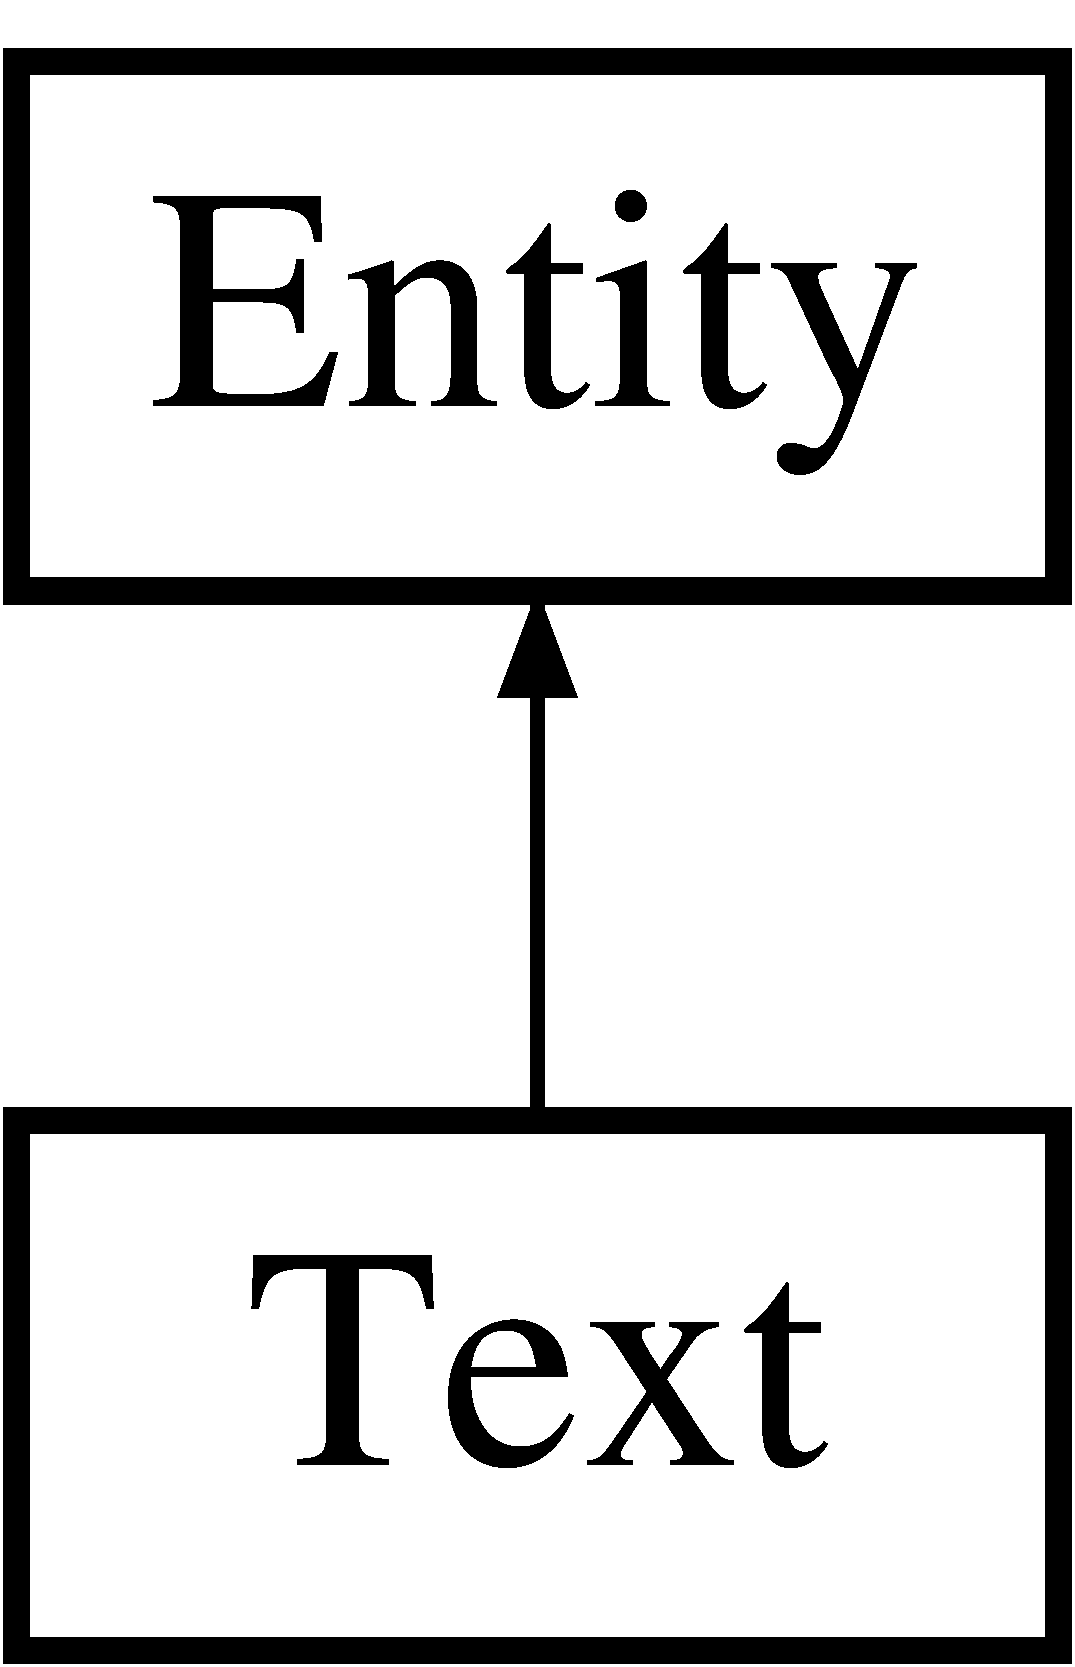
\includegraphics[height=2.000000cm]{class_text}
\end{center}
\end{figure}
\subsection*{Public Member Functions}
\begin{DoxyCompactItemize}
\item 
\hyperlink{class_text_ab3e26143fccc52699bcc5149cae852bc}{Text} ()
\begin{DoxyCompactList}\small\item\em Constructor of the \hyperlink{class_text}{Text}. \end{DoxyCompactList}\item 
\mbox{\Hypertarget{class_text_a2d49e5c280e205125b149f7777ae30c7}\label{class_text_a2d49e5c280e205125b149f7777ae30c7}} 
virtual \hyperlink{class_text_a2d49e5c280e205125b149f7777ae30c7}{$\sim$\+Text} ()
\begin{DoxyCompactList}\small\item\em Destructor of the \hyperlink{class_text}{Text}. \end{DoxyCompactList}\item 
\mbox{\Hypertarget{class_text_a5604f1f74fd487d2972d024575497484}\label{class_text_a5604f1f74fd487d2972d024575497484}} 
virtual void \hyperlink{class_text_a5604f1f74fd487d2972d024575497484}{update} (float delta\+Time)
\begin{DoxyCompactList}\small\item\em empty update function \end{DoxyCompactList}\item 
void \hyperlink{class_text_afdd312f98458f1bb34efd9112600cf2d}{clear\+Message} ()
\begin{DoxyCompactList}\small\item\em clears all Sprites for characters \end{DoxyCompactList}\item 
std\+::string \hyperlink{class_text_af104dcc0d17a6c0d211eebd034fd1e19}{message} ()
\begin{DoxyCompactList}\small\item\em message getter \end{DoxyCompactList}\item 
void \hyperlink{class_text_abebd1a39cf62aab521a0a43657c63570}{message} (std\+::string m)
\begin{DoxyCompactList}\small\item\em message setter also creates Characters \end{DoxyCompactList}\item 
void \hyperlink{class_text_a0138a1f302a7a68eca9373413463ae43}{message} (std\+::string m, \hyperlink{struct_r_g_b_a_color}{R\+G\+B\+A\+Color} c)
\begin{DoxyCompactList}\small\item\em message setter also creates Characters \end{DoxyCompactList}\end{DoxyCompactItemize}
\subsection*{Additional Inherited Members}


\subsection{Detailed Description}
The \hyperlink{class_text}{Text} class is a collection of drawable Characters. 

\subsection{Constructor \& Destructor Documentation}
\mbox{\Hypertarget{class_text_ab3e26143fccc52699bcc5149cae852bc}\label{class_text_ab3e26143fccc52699bcc5149cae852bc}} 
\index{Text@{Text}!Text@{Text}}
\index{Text@{Text}!Text@{Text}}
\subsubsection{\texorpdfstring{Text()}{Text()}}
{\footnotesize\ttfamily Text\+::\+Text (\begin{DoxyParamCaption}{ }\end{DoxyParamCaption})}



Constructor of the \hyperlink{class_text}{Text}. 

This file is part of a demo that shows how to use R\+T2D, a 2D Open\+GL framework.


\begin{DoxyItemize}
\item Copyright 2015 Rik Teerling \href{mailto:rik@onandoffables.com}{\tt rik@onandoffables.\+com}
\begin{DoxyItemize}
\item Initial commit 
\end{DoxyItemize}
\end{DoxyItemize}

\subsection{Member Function Documentation}
\mbox{\Hypertarget{class_text_afdd312f98458f1bb34efd9112600cf2d}\label{class_text_afdd312f98458f1bb34efd9112600cf2d}} 
\index{Text@{Text}!clear\+Message@{clear\+Message}}
\index{clear\+Message@{clear\+Message}!Text@{Text}}
\subsubsection{\texorpdfstring{clear\+Message()}{clearMessage()}}
{\footnotesize\ttfamily void Text\+::clear\+Message (\begin{DoxyParamCaption}{ }\end{DoxyParamCaption})}



clears all Sprites for characters 

\begin{DoxyReturn}{Returns}
void 
\end{DoxyReturn}
\mbox{\Hypertarget{class_text_af104dcc0d17a6c0d211eebd034fd1e19}\label{class_text_af104dcc0d17a6c0d211eebd034fd1e19}} 
\index{Text@{Text}!message@{message}}
\index{message@{message}!Text@{Text}}
\subsubsection{\texorpdfstring{message()}{message()}\hspace{0.1cm}{\footnotesize\ttfamily [1/3]}}
{\footnotesize\ttfamily std\+::string Text\+::message (\begin{DoxyParamCaption}{ }\end{DoxyParamCaption})\hspace{0.3cm}{\ttfamily [inline]}}



message getter 

\begin{DoxyReturn}{Returns}
std\+::string \+\_\+message 
\end{DoxyReturn}
\mbox{\Hypertarget{class_text_abebd1a39cf62aab521a0a43657c63570}\label{class_text_abebd1a39cf62aab521a0a43657c63570}} 
\index{Text@{Text}!message@{message}}
\index{message@{message}!Text@{Text}}
\subsubsection{\texorpdfstring{message()}{message()}\hspace{0.1cm}{\footnotesize\ttfamily [2/3]}}
{\footnotesize\ttfamily void Text\+::message (\begin{DoxyParamCaption}\item[{std\+::string}]{m }\end{DoxyParamCaption})}



message setter also creates Characters 


\begin{DoxyParams}{Parameters}
{\em m} & the message to be created \\
\hline
\end{DoxyParams}
\begin{DoxyReturn}{Returns}
void 
\end{DoxyReturn}
\mbox{\Hypertarget{class_text_a0138a1f302a7a68eca9373413463ae43}\label{class_text_a0138a1f302a7a68eca9373413463ae43}} 
\index{Text@{Text}!message@{message}}
\index{message@{message}!Text@{Text}}
\subsubsection{\texorpdfstring{message()}{message()}\hspace{0.1cm}{\footnotesize\ttfamily [3/3]}}
{\footnotesize\ttfamily void Text\+::message (\begin{DoxyParamCaption}\item[{std\+::string}]{m,  }\item[{\hyperlink{struct_r_g_b_a_color}{R\+G\+B\+A\+Color}}]{c }\end{DoxyParamCaption})}



message setter also creates Characters 


\begin{DoxyParams}{Parameters}
{\em m} & the message to be created \\
\hline
{\em c} & the color of the message to be created \\
\hline
\end{DoxyParams}
\begin{DoxyReturn}{Returns}
void 
\end{DoxyReturn}


The documentation for this class was generated from the following files\+:\begin{DoxyCompactItemize}
\item 
\hyperlink{text_8h}{text.\+h}\item 
text.\+cpp\end{DoxyCompactItemize}

\hypertarget{class_texture}{}\section{Texture Class Reference}
\label{class_texture}\index{Texture@{Texture}}


The \hyperlink{class_texture}{Texture} class loads images from files and converts them to Open\+GL textures.  




{\ttfamily \#include $<$texture.\+h$>$}

\subsection*{Public Member Functions}
\begin{DoxyCompactItemize}
\item 
\hyperlink{class_texture_a6c275e3f186675ff6ed73ccf970e552f}{Texture} ()
\begin{DoxyCompactList}\small\item\em Constructor of the \hyperlink{class_texture}{Texture}. \end{DoxyCompactList}\item 
\mbox{\Hypertarget{class_texture_a09c4bcb7462f64c1d20fa69dba3cee8a}\label{class_texture_a09c4bcb7462f64c1d20fa69dba3cee8a}} 
virtual \hyperlink{class_texture_a09c4bcb7462f64c1d20fa69dba3cee8a}{$\sim$\+Texture} ()
\begin{DoxyCompactList}\small\item\em Destructor of the \hyperlink{class_texture}{Texture}. \end{DoxyCompactList}\item 
G\+Luint \hyperlink{class_texture_a0c27269ad25e0d90b7bab79deaf39769}{get\+G\+L\+Texture} ()
\begin{DoxyCompactList}\small\item\em get the Open\+GL texture \end{DoxyCompactList}\item 
\hyperlink{struct_pixel_buffer}{Pixel\+Buffer} $\ast$ \hyperlink{class_texture_a6eb92d5d1c82b77fd2ced5c1b767dca1}{pixels} ()
\begin{DoxyCompactList}\small\item\em get the \hyperlink{struct_pixel_buffer}{Pixel\+Buffer} \end{DoxyCompactList}\item 
int \hyperlink{class_texture_a692f72a0e68a9ffa63d1a2e39644e7df}{width} ()
\begin{DoxyCompactList}\small\item\em get the width of the Open\+GL texture \end{DoxyCompactList}\item 
int \hyperlink{class_texture_a313a22ab82d389b2cb36fdb5cff40ecd}{height} ()
\begin{DoxyCompactList}\small\item\em get the height of the Open\+GL texture \end{DoxyCompactList}\item 
int \hyperlink{class_texture_a9e69c0d8b6e28dad8a9bb0ceb0af5da7}{depth} ()
\begin{DoxyCompactList}\small\item\em bytes per pixel. 3=R\+GB, 4=R\+G\+BA. \end{DoxyCompactList}\item 
G\+Luint \hyperlink{class_texture_a55975532738a6fab41ef8ad793d6a0ad}{load\+T\+G\+A\+Image} (const std\+::string \&filename, int filter, int wrap)
\begin{DoxyCompactList}\small\item\em load an image from file (tga only) \end{DoxyCompactList}\item 
int \hyperlink{class_texture_afe34cd10fffd2afbd2d9748f2a21acbb}{write\+T\+G\+A\+Image} (\hyperlink{struct_pixel_buffer}{Pixel\+Buffer} $\ast$\hyperlink{class_texture_a6eb92d5d1c82b77fd2ced5c1b767dca1}{pixels})
\begin{DoxyCompactList}\small\item\em write an image to file (tga only) \end{DoxyCompactList}\item 
G\+Luint \hyperlink{class_texture_a4efabecf7657384b7b6cb4e6f1b8a62f}{create\+White\+Pixels} (int \hyperlink{class_texture_a692f72a0e68a9ffa63d1a2e39644e7df}{width}, int \hyperlink{class_texture_a313a22ab82d389b2cb36fdb5cff40ecd}{height})
\begin{DoxyCompactList}\small\item\em create a width x height white \hyperlink{struct_pixel_buffer}{Pixel\+Buffer} \& G\+Lpixeldata \end{DoxyCompactList}\item 
void \hyperlink{class_texture_a2766d07d7c01aad338b457ae9d844e71}{create\+From\+Buffer} (\hyperlink{struct_pixel_buffer}{Pixel\+Buffer} $\ast$\hyperlink{class_texture_a6eb92d5d1c82b77fd2ced5c1b767dca1}{pixels})
\begin{DoxyCompactList}\small\item\em create a \hyperlink{class_texture}{Texture} from a \hyperlink{struct_pixel_buffer}{Pixel\+Buffer} \end{DoxyCompactList}\item 
unsigned char \hyperlink{class_texture_a13c3996f10cc236ee21b517da8501973}{warranty} ()
\begin{DoxyCompactList}\small\item\em get the warranty bit \end{DoxyCompactList}\end{DoxyCompactItemize}


\subsection{Detailed Description}
The \hyperlink{class_texture}{Texture} class loads images from files and converts them to Open\+GL textures. 

\subsection{Constructor \& Destructor Documentation}
\mbox{\Hypertarget{class_texture_a6c275e3f186675ff6ed73ccf970e552f}\label{class_texture_a6c275e3f186675ff6ed73ccf970e552f}} 
\index{Texture@{Texture}!Texture@{Texture}}
\index{Texture@{Texture}!Texture@{Texture}}
\subsubsection{\texorpdfstring{Texture()}{Texture()}}
{\footnotesize\ttfamily Texture\+::\+Texture (\begin{DoxyParamCaption}{ }\end{DoxyParamCaption})}



Constructor of the \hyperlink{class_texture}{Texture}. 

This file is part of R\+T2D, a 2D Open\+GL framework.


\begin{DoxyItemize}
\item Copyright 2015 Rik Teerling \href{mailto:rik@onandoffables.com}{\tt rik@onandoffables.\+com}
\begin{DoxyItemize}
\item Initial commit 
\end{DoxyItemize}
\end{DoxyItemize}

\subsection{Member Function Documentation}
\mbox{\Hypertarget{class_texture_a2766d07d7c01aad338b457ae9d844e71}\label{class_texture_a2766d07d7c01aad338b457ae9d844e71}} 
\index{Texture@{Texture}!create\+From\+Buffer@{create\+From\+Buffer}}
\index{create\+From\+Buffer@{create\+From\+Buffer}!Texture@{Texture}}
\subsubsection{\texorpdfstring{create\+From\+Buffer()}{createFromBuffer()}}
{\footnotesize\ttfamily void Texture\+::create\+From\+Buffer (\begin{DoxyParamCaption}\item[{\hyperlink{struct_pixel_buffer}{Pixel\+Buffer} $\ast$}]{pixels }\end{DoxyParamCaption})}



create a \hyperlink{class_texture}{Texture} from a \hyperlink{struct_pixel_buffer}{Pixel\+Buffer} 


\begin{DoxyParams}{Parameters}
{\em pixels} & a \hyperlink{struct_pixel_buffer}{Pixel\+Buffer} pointer \\
\hline
\end{DoxyParams}
\begin{DoxyReturn}{Returns}
G\+Luint \+\_\+texture, 0 if failed 
\end{DoxyReturn}
\mbox{\Hypertarget{class_texture_a4efabecf7657384b7b6cb4e6f1b8a62f}\label{class_texture_a4efabecf7657384b7b6cb4e6f1b8a62f}} 
\index{Texture@{Texture}!create\+White\+Pixels@{create\+White\+Pixels}}
\index{create\+White\+Pixels@{create\+White\+Pixels}!Texture@{Texture}}
\subsubsection{\texorpdfstring{create\+White\+Pixels()}{createWhitePixels()}}
{\footnotesize\ttfamily G\+Luint Texture\+::create\+White\+Pixels (\begin{DoxyParamCaption}\item[{int}]{width,  }\item[{int}]{height }\end{DoxyParamCaption})}



create a width x height white \hyperlink{struct_pixel_buffer}{Pixel\+Buffer} \& G\+Lpixeldata 


\begin{DoxyParams}{Parameters}
{\em width} & the width of the white \hyperlink{class_texture}{Texture} \\
\hline
{\em height} & the height of the white \hyperlink{class_texture}{Texture} \\
\hline
\end{DoxyParams}
\begin{DoxyReturn}{Returns}
G\+Luint \+\_\+texture, 0 if failed 
\end{DoxyReturn}
\mbox{\Hypertarget{class_texture_a9e69c0d8b6e28dad8a9bb0ceb0af5da7}\label{class_texture_a9e69c0d8b6e28dad8a9bb0ceb0af5da7}} 
\index{Texture@{Texture}!depth@{depth}}
\index{depth@{depth}!Texture@{Texture}}
\subsubsection{\texorpdfstring{depth()}{depth()}}
{\footnotesize\ttfamily int Texture\+::depth (\begin{DoxyParamCaption}{ }\end{DoxyParamCaption})\hspace{0.3cm}{\ttfamily [inline]}}



bytes per pixel. 3=R\+GB, 4=R\+G\+BA. 

\begin{DoxyReturn}{Returns}
int \+\_\+depth 
\end{DoxyReturn}
\mbox{\Hypertarget{class_texture_a0c27269ad25e0d90b7bab79deaf39769}\label{class_texture_a0c27269ad25e0d90b7bab79deaf39769}} 
\index{Texture@{Texture}!get\+G\+L\+Texture@{get\+G\+L\+Texture}}
\index{get\+G\+L\+Texture@{get\+G\+L\+Texture}!Texture@{Texture}}
\subsubsection{\texorpdfstring{get\+G\+L\+Texture()}{getGLTexture()}}
{\footnotesize\ttfamily G\+Luint Texture\+::get\+G\+L\+Texture (\begin{DoxyParamCaption}{ }\end{DoxyParamCaption})\hspace{0.3cm}{\ttfamily [inline]}}



get the Open\+GL texture 

\begin{DoxyReturn}{Returns}
G\+Luint \+\_\+texture 
\end{DoxyReturn}
\mbox{\Hypertarget{class_texture_a313a22ab82d389b2cb36fdb5cff40ecd}\label{class_texture_a313a22ab82d389b2cb36fdb5cff40ecd}} 
\index{Texture@{Texture}!height@{height}}
\index{height@{height}!Texture@{Texture}}
\subsubsection{\texorpdfstring{height()}{height()}}
{\footnotesize\ttfamily int Texture\+::height (\begin{DoxyParamCaption}{ }\end{DoxyParamCaption})\hspace{0.3cm}{\ttfamily [inline]}}



get the height of the Open\+GL texture 

\begin{DoxyReturn}{Returns}
int \+\_\+height 
\end{DoxyReturn}
\mbox{\Hypertarget{class_texture_a55975532738a6fab41ef8ad793d6a0ad}\label{class_texture_a55975532738a6fab41ef8ad793d6a0ad}} 
\index{Texture@{Texture}!load\+T\+G\+A\+Image@{load\+T\+G\+A\+Image}}
\index{load\+T\+G\+A\+Image@{load\+T\+G\+A\+Image}!Texture@{Texture}}
\subsubsection{\texorpdfstring{load\+T\+G\+A\+Image()}{loadTGAImage()}}
{\footnotesize\ttfamily G\+Luint Texture\+::load\+T\+G\+A\+Image (\begin{DoxyParamCaption}\item[{const std\+::string \&}]{filename,  }\item[{int}]{filter,  }\item[{int}]{wrap }\end{DoxyParamCaption})}



load an image from file (tga only) 


\begin{DoxyParams}{Parameters}
{\em filename} & the path to the image \\
\hline
{\em filter} & the filter \\
\hline
{\em wrap} & the wrap \\
\hline
\end{DoxyParams}
\begin{DoxyReturn}{Returns}
G\+Luint \+\_\+texture, 0 if failed 
\end{DoxyReturn}
\mbox{\Hypertarget{class_texture_a6eb92d5d1c82b77fd2ced5c1b767dca1}\label{class_texture_a6eb92d5d1c82b77fd2ced5c1b767dca1}} 
\index{Texture@{Texture}!pixels@{pixels}}
\index{pixels@{pixels}!Texture@{Texture}}
\subsubsection{\texorpdfstring{pixels()}{pixels()}}
{\footnotesize\ttfamily \hyperlink{struct_pixel_buffer}{Pixel\+Buffer}$\ast$ Texture\+::pixels (\begin{DoxyParamCaption}{ }\end{DoxyParamCaption})\hspace{0.3cm}{\ttfamily [inline]}}



get the \hyperlink{struct_pixel_buffer}{Pixel\+Buffer} 

\begin{DoxyReturn}{Returns}
Pixel\+Buffer$\ast$ \+\_\+pixelbuffer 
\end{DoxyReturn}
\mbox{\Hypertarget{class_texture_a13c3996f10cc236ee21b517da8501973}\label{class_texture_a13c3996f10cc236ee21b517da8501973}} 
\index{Texture@{Texture}!warranty@{warranty}}
\index{warranty@{warranty}!Texture@{Texture}}
\subsubsection{\texorpdfstring{warranty()}{warranty()}}
{\footnotesize\ttfamily unsigned char Texture\+::warranty (\begin{DoxyParamCaption}{ }\end{DoxyParamCaption})\hspace{0.3cm}{\ttfamily [inline]}}



get the warranty bit 

\begin{DoxyReturn}{Returns}
unsigned char \+\_\+warrantybit 
\end{DoxyReturn}
\mbox{\Hypertarget{class_texture_a692f72a0e68a9ffa63d1a2e39644e7df}\label{class_texture_a692f72a0e68a9ffa63d1a2e39644e7df}} 
\index{Texture@{Texture}!width@{width}}
\index{width@{width}!Texture@{Texture}}
\subsubsection{\texorpdfstring{width()}{width()}}
{\footnotesize\ttfamily int Texture\+::width (\begin{DoxyParamCaption}{ }\end{DoxyParamCaption})\hspace{0.3cm}{\ttfamily [inline]}}



get the width of the Open\+GL texture 

\begin{DoxyReturn}{Returns}
int \+\_\+width 
\end{DoxyReturn}
\mbox{\Hypertarget{class_texture_afe34cd10fffd2afbd2d9748f2a21acbb}\label{class_texture_afe34cd10fffd2afbd2d9748f2a21acbb}} 
\index{Texture@{Texture}!write\+T\+G\+A\+Image@{write\+T\+G\+A\+Image}}
\index{write\+T\+G\+A\+Image@{write\+T\+G\+A\+Image}!Texture@{Texture}}
\subsubsection{\texorpdfstring{write\+T\+G\+A\+Image()}{writeTGAImage()}}
{\footnotesize\ttfamily int Texture\+::write\+T\+G\+A\+Image (\begin{DoxyParamCaption}\item[{\hyperlink{struct_pixel_buffer}{Pixel\+Buffer} $\ast$}]{pixels }\end{DoxyParamCaption})}



write an image to file (tga only) 


\begin{DoxyParams}{Parameters}
{\em pixels} & the \hyperlink{struct_pixel_buffer}{Pixel\+Buffer} to write \\
\hline
\end{DoxyParams}
\begin{DoxyReturn}{Returns}
int 0 if failed 
\end{DoxyReturn}


The documentation for this class was generated from the following files\+:\begin{DoxyCompactItemize}
\item 
\hyperlink{texture_8h}{texture.\+h}\item 
texture.\+cpp\end{DoxyCompactItemize}

\hypertarget{class_timer}{}\section{Timer Class Reference}
\label{class_timer}\index{Timer@{Timer}}


The \hyperlink{class_timer}{Timer} class keeps track of time.  




{\ttfamily \#include $<$timer.\+h$>$}

\subsection*{Public Member Functions}
\begin{DoxyCompactItemize}
\item 
\hyperlink{class_timer_a5f16e8da27d2a5a5242dead46de05d97}{Timer} ()
\begin{DoxyCompactList}\small\item\em Constructor of the \hyperlink{class_timer}{Timer}. \end{DoxyCompactList}\item 
\mbox{\Hypertarget{class_timer_a14fa469c4c295c5fa6e66a4ad1092146}\label{class_timer_a14fa469c4c295c5fa6e66a4ad1092146}} 
virtual \hyperlink{class_timer_a14fa469c4c295c5fa6e66a4ad1092146}{$\sim$\+Timer} ()
\begin{DoxyCompactList}\small\item\em Destructor of the \hyperlink{class_timer}{Timer}. \end{DoxyCompactList}\item 
\mbox{\Hypertarget{class_timer_a3a8b5272198d029779dc9302a54305a8}\label{class_timer_a3a8b5272198d029779dc9302a54305a8}} 
void \hyperlink{class_timer_a3a8b5272198d029779dc9302a54305a8}{start} ()
\begin{DoxyCompactList}\small\item\em start the \hyperlink{class_timer}{Timer} \end{DoxyCompactList}\item 
\mbox{\Hypertarget{class_timer_a63f0eb44b27402196590a03781515dba}\label{class_timer_a63f0eb44b27402196590a03781515dba}} 
void \hyperlink{class_timer_a63f0eb44b27402196590a03781515dba}{stop} ()
\begin{DoxyCompactList}\small\item\em stop the \hyperlink{class_timer}{Timer} \end{DoxyCompactList}\item 
\mbox{\Hypertarget{class_timer_a0289effad7b573c508bc27e405900a23}\label{class_timer_a0289effad7b573c508bc27e405900a23}} 
void \hyperlink{class_timer_a0289effad7b573c508bc27e405900a23}{pause} ()
\begin{DoxyCompactList}\small\item\em pause the \hyperlink{class_timer}{Timer} \end{DoxyCompactList}\item 
\mbox{\Hypertarget{class_timer_aa4dd50d7ed48ac73efed2950749d35d6}\label{class_timer_aa4dd50d7ed48ac73efed2950749d35d6}} 
void \hyperlink{class_timer_aa4dd50d7ed48ac73efed2950749d35d6}{unpause} ()
\begin{DoxyCompactList}\small\item\em unpause the \hyperlink{class_timer}{Timer} \end{DoxyCompactList}\item 
\mbox{\Hypertarget{class_timer_a6d78b6933862786b1851fef22489245c}\label{class_timer_a6d78b6933862786b1851fef22489245c}} 
void \hyperlink{class_timer_a6d78b6933862786b1851fef22489245c}{paused} (bool b)
\begin{DoxyCompactList}\small\item\em set paused or not \end{DoxyCompactList}\item 
\mbox{\Hypertarget{class_timer_a058dd4c31bf7af5a0282c405e3af4d7a}\label{class_timer_a058dd4c31bf7af5a0282c405e3af4d7a}} 
bool \hyperlink{class_timer_a058dd4c31bf7af5a0282c405e3af4d7a}{paused} ()
\begin{DoxyCompactList}\small\item\em paused or not \end{DoxyCompactList}\item 
double \hyperlink{class_timer_a045bb982f9132c9043fb10be01370485}{seconds} ()
\begin{DoxyCompactList}\small\item\em the number of seconds passed since \hyperlink{class_timer_a3a8b5272198d029779dc9302a54305a8}{Timer\+::start()} \end{DoxyCompactList}\end{DoxyCompactItemize}


\subsection{Detailed Description}
The \hyperlink{class_timer}{Timer} class keeps track of time. 

\subsection{Constructor \& Destructor Documentation}
\mbox{\Hypertarget{class_timer_a5f16e8da27d2a5a5242dead46de05d97}\label{class_timer_a5f16e8da27d2a5a5242dead46de05d97}} 
\index{Timer@{Timer}!Timer@{Timer}}
\index{Timer@{Timer}!Timer@{Timer}}
\subsubsection{\texorpdfstring{Timer()}{Timer()}}
{\footnotesize\ttfamily Timer\+::\+Timer (\begin{DoxyParamCaption}{ }\end{DoxyParamCaption})}



Constructor of the \hyperlink{class_timer}{Timer}. 

This file is part of R\+T2D, a 2D Open\+GL framework.


\begin{DoxyItemize}
\item Copyright 2015 Rik Teerling \href{mailto:rik@onandoffables.com}{\tt rik@onandoffables.\+com}
\begin{DoxyItemize}
\item Initial commit 
\end{DoxyItemize}
\end{DoxyItemize}

\subsection{Member Function Documentation}
\mbox{\Hypertarget{class_timer_a045bb982f9132c9043fb10be01370485}\label{class_timer_a045bb982f9132c9043fb10be01370485}} 
\index{Timer@{Timer}!seconds@{seconds}}
\index{seconds@{seconds}!Timer@{Timer}}
\subsubsection{\texorpdfstring{seconds()}{seconds()}}
{\footnotesize\ttfamily double Timer\+::seconds (\begin{DoxyParamCaption}{ }\end{DoxyParamCaption})}



the number of seconds passed since \hyperlink{class_timer_a3a8b5272198d029779dc9302a54305a8}{Timer\+::start()} 

\begin{DoxyReturn}{Returns}
double time in seconds 
\end{DoxyReturn}


The documentation for this class was generated from the following files\+:\begin{DoxyCompactItemize}
\item 
\hyperlink{timer_8h}{timer.\+h}\item 
timer.\+cpp\end{DoxyCompactItemize}

\hypertarget{class_vector_x__t}{}\section{Vector\+X\+\_\+t$<$ T $>$ Class Template Reference}
\label{class_vector_x__t}\index{Vector\+X\+\_\+t$<$ T $>$@{Vector\+X\+\_\+t$<$ T $>$}}


A helper class to calculate distances and angles.  




{\ttfamily \#include $<$vectorx.\+h$>$}

Inheritance diagram for Vector\+X\+\_\+t$<$ T $>$\+:\begin{figure}[H]
\begin{center}
\leavevmode
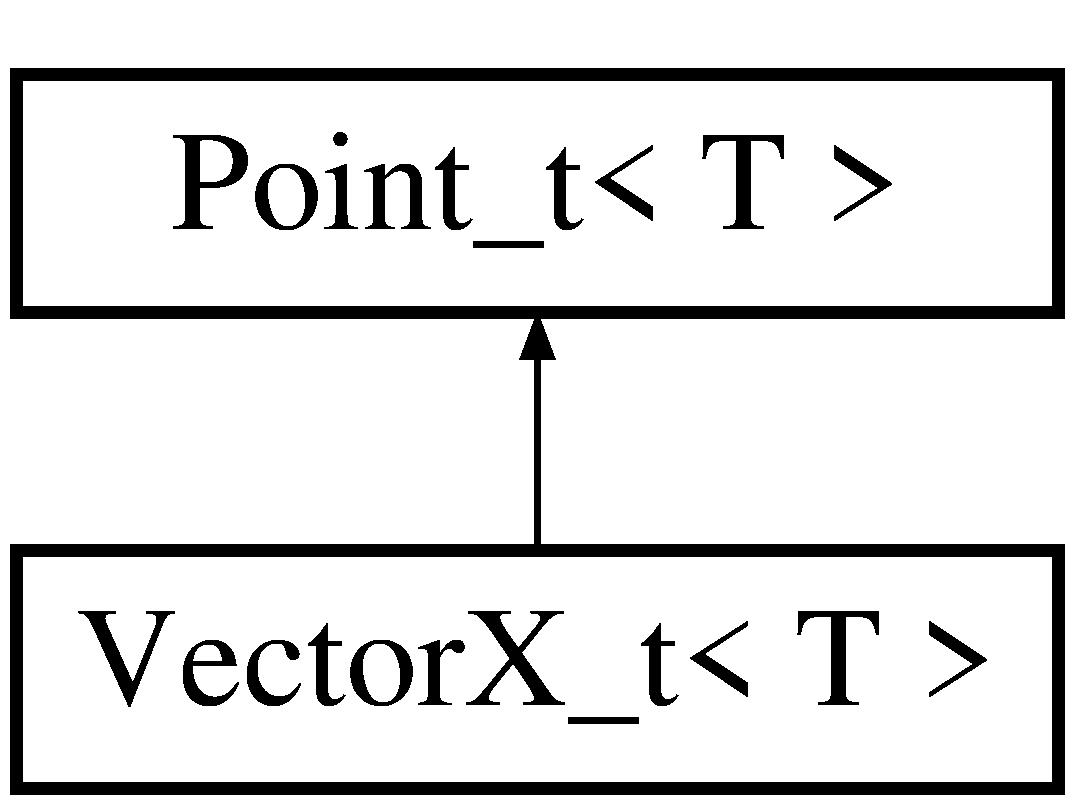
\includegraphics[height=2.000000cm]{class_vector_x__t}
\end{center}
\end{figure}
\subsection*{Public Member Functions}
\begin{DoxyCompactItemize}
\item 
\hyperlink{class_vector_x__t_a0afaded32c122f68359ed9aa789978f2}{Vector\+X\+\_\+t} ()
\begin{DoxyCompactList}\small\item\em Default Vector\+\_\+t$<$\+T$>$ constructor. \end{DoxyCompactList}\item 
\hyperlink{class_vector_x__t_a3e9c4344b74f4a74924188c9d7ee6b16}{Vector\+X\+\_\+t} (T xx, T yy)
\begin{DoxyCompactList}\small\item\em Creates a Vector2 with endpoint xx,yy. \end{DoxyCompactList}\item 
\hyperlink{class_vector_x__t_a11ee21d75512d8ecf7cbb21b97e4b47e}{Vector\+X\+\_\+t} (T xx, T yy, T zz)
\begin{DoxyCompactList}\small\item\em Creates a Vector3 with endpoint xx,yy,zz. \end{DoxyCompactList}\item 
\hyperlink{class_vector_x__t_a25ef303a780ddfd52572d95c232d2a5b}{Vector\+X\+\_\+t} (\hyperlink{class_point__t}{Point\+\_\+t}$<$ T $>$ p)
\begin{DoxyCompactList}\small\item\em Creates a Vector\+\_\+t$<$\+T$>$ with endpoint Point\+\_\+t$<$\+T$>$ p. \end{DoxyCompactList}\item 
\hyperlink{class_vector_x__t_a8ac4f12ebd7673a4b3b7cf86e842c912}{Vector\+X\+\_\+t} (\hyperlink{class_point__t}{Point\+\_\+t}$<$ T $>$ begin, \hyperlink{class_point__t}{Point\+\_\+t}$<$ T $>$ end)
\begin{DoxyCompactList}\small\item\em Creates a Vector\+\_\+t$<$\+T$>$ with startingpoint begin and endpoint end. \end{DoxyCompactList}\item 
virtual \hyperlink{class_vector_x__t_a91e541bc8a28a206c0caaefee09c4fdc}{$\sim$\+Vector\+X\+\_\+t} ()
\begin{DoxyCompactList}\small\item\em This is the Vector\+\_\+t$<$\+T$>$ destructor. \end{DoxyCompactList}\item 
const T \hyperlink{class_vector_x__t_aa1548451f4620694a671d9b15be69ba2}{get\+Length} () const
\begin{DoxyCompactList}\small\item\em Get the length of the Vector\+\_\+t$<$\+T$>$ \end{DoxyCompactList}\item 
const T \hyperlink{class_vector_x__t_a2b6ed2553246864a1f903619de4e0786}{get\+Length\+Squared} () const
\begin{DoxyCompactList}\small\item\em Get the squared length of the Vector\+\_\+t$<$\+T$>$ \end{DoxyCompactList}\item 
const T \hyperlink{class_vector_x__t_a7e497c0abad76724767e78644ff91e35}{get\+Angle} () const
\begin{DoxyCompactList}\small\item\em Get the angle of the Vector2 in radians on the X-\/axis. \end{DoxyCompactList}\item 
const T \hyperlink{class_vector_x__t_abdee14870829077f912a2e5b85ceb51a}{get\+Angle\+Deg} () const
\begin{DoxyCompactList}\small\item\em Get the angle of the Vector2 in degrees on the X-\/axis. \end{DoxyCompactList}\item 
const T \hyperlink{class_vector_x__t_a875b1e98058eafffead7e4a0e39496f9}{get\+Angle} (const \hyperlink{class_vector_x__t}{Vector\+X\+\_\+t}$<$ T $>$ \&other) const
\begin{DoxyCompactList}\small\item\em Get the angle between this Vector\+\_\+t$<$\+T$>$, and another Vector\+\_\+t$<$\+T$>$ in radians. \end{DoxyCompactList}\item 
const T \hyperlink{class_vector_x__t_a936a9063f46982c8837b88c6a16526bf}{get\+Angle\+Deg} (const \hyperlink{class_vector_x__t}{Vector\+X\+\_\+t}$<$ T $>$ \&other) const
\begin{DoxyCompactList}\small\item\em Get the angle between this Vector\+\_\+t$<$\+T$>$, and another Vector\+\_\+t$<$\+T$>$ in degrees. \end{DoxyCompactList}\item 
const \hyperlink{class_vector_x__t}{Vector\+X\+\_\+t}$<$ T $>$ \hyperlink{class_vector_x__t_af977e73b4611bededc322a113ad2b523}{get\+Normalized} () const
\begin{DoxyCompactList}\small\item\em Get the normalized Vector\+\_\+t$<$\+T$>$. \end{DoxyCompactList}\item 
\mbox{\Hypertarget{class_vector_x__t_a11fc8d9232f89ad0b572fcaff6895814}\label{class_vector_x__t_a11fc8d9232f89ad0b572fcaff6895814}} 
void \hyperlink{class_vector_x__t_a11fc8d9232f89ad0b572fcaff6895814}{normalize} ()
\begin{DoxyCompactList}\small\item\em normalize this Vector\+\_\+t$<$\+T$>$ \end{DoxyCompactList}\item 
\mbox{\Hypertarget{class_vector_x__t_abf57f54eabe52a159804689ccd80b9c4}\label{class_vector_x__t_abf57f54eabe52a159804689ccd80b9c4}} 
void \hyperlink{class_vector_x__t_abf57f54eabe52a159804689ccd80b9c4}{lerp} (T frac)
\begin{DoxyCompactList}\small\item\em Get a lerped Vector\+\_\+t$<$\+T$>$ according to some fraction (between 0 and 1) \end{DoxyCompactList}\item 
const \hyperlink{class_vector_x__t}{Vector\+X\+\_\+t}$<$ T $>$ \hyperlink{class_vector_x__t_a2b5339021a3287a60081537d0e0a75d7}{get\+Lerped} (T frac) const
\begin{DoxyCompactList}\small\item\em Get a copy of a lerped Vector\+\_\+t$<$\+T$>$ according to some fraction (between 0 and 1) \end{DoxyCompactList}\item 
const T \hyperlink{class_vector_x__t_a47edb26aa302ab3611ec850f56b1a0f0}{dot} (const \hyperlink{class_vector_x__t}{Vector\+X\+\_\+t}$<$ T $>$ \&other) const
\begin{DoxyCompactList}\small\item\em Get the dot product of this and another Vector\+\_\+t$<$\+T$>$. \end{DoxyCompactList}\item 
const \hyperlink{class_vector_x__t}{Vector\+X\+\_\+t}$<$ T $>$ \hyperlink{class_vector_x__t_a8384a54196c5416ccca9312a87f23321}{cross} (const \hyperlink{class_vector_x__t}{Vector\+X\+\_\+t}$<$ T $>$ \&other) const
\begin{DoxyCompactList}\small\item\em Get the cross product of this and another Vector3. This only makes sense with a Vector3. \end{DoxyCompactList}\item 
void \hyperlink{class_vector_x__t_ad4e572fc98fe4d786b907598b2c8eb77}{rotate} (T angle)
\begin{DoxyCompactList}\small\item\em Rotate this Vector2 in radians. \end{DoxyCompactList}\item 
void \hyperlink{class_vector_x__t_a3ff22c065f96081f36844f175822117b}{rotation} (T angle)
\begin{DoxyCompactList}\small\item\em set the Rotation of this Vector2 in radians. \end{DoxyCompactList}\item 
void \hyperlink{class_vector_x__t_a06dd763262cfd0779011a0a292ba2143}{rotate\+Deg} (T angle)
\begin{DoxyCompactList}\small\item\em Rotate this Vector2 in degrees. \end{DoxyCompactList}\item 
void \hyperlink{class_vector_x__t_a9f02a5c0c808aa2270e443031ba1e9e0}{rotation\+Deg} (T angle)
\begin{DoxyCompactList}\small\item\em set the Rotation of this Vector2 in degrees. \end{DoxyCompactList}\item 
const \hyperlink{class_vector_x__t}{Vector\+X\+\_\+t}$<$ T $>$ \hyperlink{class_vector_x__t_a73fc65bea5601dc510b720305fab02b5}{get\+Rotated} (T angle) const
\begin{DoxyCompactList}\small\item\em Get a rotated copy of this Vector2 in radians. \end{DoxyCompactList}\item 
const \hyperlink{class_vector_x__t}{Vector\+X\+\_\+t}$<$ T $>$ \hyperlink{class_vector_x__t_ae1d1ebad5cbaa4430f9a6e230b98c99e}{get\+Rotated\+Deg} (T angle) const
\begin{DoxyCompactList}\small\item\em Get a Rotated copy of this Vector2 in degrees. \end{DoxyCompactList}\item 
void \hyperlink{class_vector_x__t_a2a4914eef4789c14c1c78b235b298565}{limit} (T amount)
\begin{DoxyCompactList}\small\item\em Limit the length of this Vector2 to the amount. \end{DoxyCompactList}\item 
const bool \hyperlink{class_vector_x__t_a4e568334b218fda51d03636310f23ab4}{operator$<$} (\hyperlink{class_vector_x__t}{Vector\+X\+\_\+t}$<$ T $>$ other) const
\begin{DoxyCompactList}\small\item\em Overloads the $<$ operator. \end{DoxyCompactList}\item 
const bool \hyperlink{class_vector_x__t_a311676a873e6851386a71d5b781d77fc}{operator$>$} (\hyperlink{class_vector_x__t}{Vector\+X\+\_\+t}$<$ T $>$ other) const
\begin{DoxyCompactList}\small\item\em Overloads the $>$ operator. \end{DoxyCompactList}\item 
const bool \hyperlink{class_vector_x__t_a4aa8b297bdb6c3e51c004520bff95f73}{operator$<$=} (\hyperlink{class_vector_x__t}{Vector\+X\+\_\+t}$<$ T $>$ other) const
\begin{DoxyCompactList}\small\item\em Overloads the $<$= operator. \end{DoxyCompactList}\item 
const bool \hyperlink{class_vector_x__t_a5e7b917f91229508634bc8ab57a3b02c}{operator$>$=} (\hyperlink{class_vector_x__t}{Vector\+X\+\_\+t}$<$ T $>$ other) const
\begin{DoxyCompactList}\small\item\em Overloads the $>$= operator. \end{DoxyCompactList}\end{DoxyCompactItemize}
\subsection*{Additional Inherited Members}


\subsection{Detailed Description}
\subsubsection*{template$<$class T$>$\newline
class Vector\+X\+\_\+t$<$ T $>$}

A helper class to calculate distances and angles. 

Extends Point. A Vector\+\_\+t$<$\+T$>$ contains the end position, but also direction. The origin is always 0,0,0

You will probably use this mostly as a Vector2. It is in fact a Vector3, but it should be transparent enough not to notice. 

\subsection{Constructor \& Destructor Documentation}
\mbox{\Hypertarget{class_vector_x__t_a0afaded32c122f68359ed9aa789978f2}\label{class_vector_x__t_a0afaded32c122f68359ed9aa789978f2}} 
\index{Vector\+X\+\_\+t@{Vector\+X\+\_\+t}!Vector\+X\+\_\+t@{Vector\+X\+\_\+t}}
\index{Vector\+X\+\_\+t@{Vector\+X\+\_\+t}!Vector\+X\+\_\+t@{Vector\+X\+\_\+t}}
\subsubsection{\texorpdfstring{Vector\+X\+\_\+t()}{VectorX\_t()}\hspace{0.1cm}{\footnotesize\ttfamily [1/5]}}
{\footnotesize\ttfamily template$<$class T $>$ \\
\hyperlink{class_vector_x__t}{Vector\+X\+\_\+t}$<$ T $>$\+::\hyperlink{class_vector_x__t}{Vector\+X\+\_\+t} (\begin{DoxyParamCaption}{ }\end{DoxyParamCaption})}



Default Vector\+\_\+t$<$\+T$>$ constructor. 

Creates a Vector\+\_\+t$<$\+T$>$ with endpoint 0,0,0 Length = 0 \mbox{\Hypertarget{class_vector_x__t_a3e9c4344b74f4a74924188c9d7ee6b16}\label{class_vector_x__t_a3e9c4344b74f4a74924188c9d7ee6b16}} 
\index{Vector\+X\+\_\+t@{Vector\+X\+\_\+t}!Vector\+X\+\_\+t@{Vector\+X\+\_\+t}}
\index{Vector\+X\+\_\+t@{Vector\+X\+\_\+t}!Vector\+X\+\_\+t@{Vector\+X\+\_\+t}}
\subsubsection{\texorpdfstring{Vector\+X\+\_\+t()}{VectorX\_t()}\hspace{0.1cm}{\footnotesize\ttfamily [2/5]}}
{\footnotesize\ttfamily template$<$class T $>$ \\
\hyperlink{class_vector_x__t}{Vector\+X\+\_\+t}$<$ T $>$\+::\hyperlink{class_vector_x__t}{Vector\+X\+\_\+t} (\begin{DoxyParamCaption}\item[{T}]{xx,  }\item[{T}]{yy }\end{DoxyParamCaption})}



Creates a Vector2 with endpoint xx,yy. 

This is an overloaded Vector2 constructor.


\begin{DoxyParams}{Parameters}
{\em xx} & The x position of the Vector2. \\
\hline
{\em yy} & The y position of the Vector2. \\
\hline
\end{DoxyParams}
\mbox{\Hypertarget{class_vector_x__t_a11ee21d75512d8ecf7cbb21b97e4b47e}\label{class_vector_x__t_a11ee21d75512d8ecf7cbb21b97e4b47e}} 
\index{Vector\+X\+\_\+t@{Vector\+X\+\_\+t}!Vector\+X\+\_\+t@{Vector\+X\+\_\+t}}
\index{Vector\+X\+\_\+t@{Vector\+X\+\_\+t}!Vector\+X\+\_\+t@{Vector\+X\+\_\+t}}
\subsubsection{\texorpdfstring{Vector\+X\+\_\+t()}{VectorX\_t()}\hspace{0.1cm}{\footnotesize\ttfamily [3/5]}}
{\footnotesize\ttfamily template$<$class T $>$ \\
\hyperlink{class_vector_x__t}{Vector\+X\+\_\+t}$<$ T $>$\+::\hyperlink{class_vector_x__t}{Vector\+X\+\_\+t} (\begin{DoxyParamCaption}\item[{T}]{xx,  }\item[{T}]{yy,  }\item[{T}]{zz }\end{DoxyParamCaption})}



Creates a Vector3 with endpoint xx,yy,zz. 

This is an overloaded Vector3 constructor.


\begin{DoxyParams}{Parameters}
{\em xx} & The x position of the Vector3. \\
\hline
{\em yy} & The y position of the Vector3. \\
\hline
{\em zz} & The z position of the Vector3. \\
\hline
\end{DoxyParams}
\mbox{\Hypertarget{class_vector_x__t_a25ef303a780ddfd52572d95c232d2a5b}\label{class_vector_x__t_a25ef303a780ddfd52572d95c232d2a5b}} 
\index{Vector\+X\+\_\+t@{Vector\+X\+\_\+t}!Vector\+X\+\_\+t@{Vector\+X\+\_\+t}}
\index{Vector\+X\+\_\+t@{Vector\+X\+\_\+t}!Vector\+X\+\_\+t@{Vector\+X\+\_\+t}}
\subsubsection{\texorpdfstring{Vector\+X\+\_\+t()}{VectorX\_t()}\hspace{0.1cm}{\footnotesize\ttfamily [4/5]}}
{\footnotesize\ttfamily template$<$class T $>$ \\
\hyperlink{class_vector_x__t}{Vector\+X\+\_\+t}$<$ T $>$\+::\hyperlink{class_vector_x__t}{Vector\+X\+\_\+t} (\begin{DoxyParamCaption}\item[{\hyperlink{class_point__t}{Point\+\_\+t}$<$ T $>$}]{p }\end{DoxyParamCaption})}



Creates a Vector\+\_\+t$<$\+T$>$ with endpoint Point\+\_\+t$<$\+T$>$ p. 

This is an overloaded Vector\+\_\+t$<$\+T$>$ constructor.


\begin{DoxyParams}{Parameters}
{\em p} & The position of the Vector\+\_\+t$<$\+T$>$ as a Point. \\
\hline
\end{DoxyParams}
\mbox{\Hypertarget{class_vector_x__t_a8ac4f12ebd7673a4b3b7cf86e842c912}\label{class_vector_x__t_a8ac4f12ebd7673a4b3b7cf86e842c912}} 
\index{Vector\+X\+\_\+t@{Vector\+X\+\_\+t}!Vector\+X\+\_\+t@{Vector\+X\+\_\+t}}
\index{Vector\+X\+\_\+t@{Vector\+X\+\_\+t}!Vector\+X\+\_\+t@{Vector\+X\+\_\+t}}
\subsubsection{\texorpdfstring{Vector\+X\+\_\+t()}{VectorX\_t()}\hspace{0.1cm}{\footnotesize\ttfamily [5/5]}}
{\footnotesize\ttfamily template$<$class T $>$ \\
\hyperlink{class_vector_x__t}{Vector\+X\+\_\+t}$<$ T $>$\+::\hyperlink{class_vector_x__t}{Vector\+X\+\_\+t} (\begin{DoxyParamCaption}\item[{\hyperlink{class_point__t}{Point\+\_\+t}$<$ T $>$}]{begin,  }\item[{\hyperlink{class_point__t}{Point\+\_\+t}$<$ T $>$}]{end }\end{DoxyParamCaption})}



Creates a Vector\+\_\+t$<$\+T$>$ with startingpoint begin and endpoint end. 

This is an overloaded Vector\+\_\+t$<$\+T$>$ constructor.


\begin{DoxyParams}{Parameters}
{\em begin} & The origin of the Vector\+\_\+t$<$\+T$>$ \\
\hline
{\em end} & The endpoint of the Vector\+\_\+t$<$\+T$>$. \\
\hline
\end{DoxyParams}
\mbox{\Hypertarget{class_vector_x__t_a91e541bc8a28a206c0caaefee09c4fdc}\label{class_vector_x__t_a91e541bc8a28a206c0caaefee09c4fdc}} 
\index{Vector\+X\+\_\+t@{Vector\+X\+\_\+t}!````~Vector\+X\+\_\+t@{$\sim$\+Vector\+X\+\_\+t}}
\index{````~Vector\+X\+\_\+t@{$\sim$\+Vector\+X\+\_\+t}!Vector\+X\+\_\+t@{Vector\+X\+\_\+t}}
\subsubsection{\texorpdfstring{$\sim$\+Vector\+X\+\_\+t()}{~VectorX\_t()}}
{\footnotesize\ttfamily template$<$class T $>$ \\
\hyperlink{class_vector_x__t}{Vector\+X\+\_\+t}$<$ T $>$\+::$\sim$\hyperlink{class_vector_x__t}{Vector\+X\+\_\+t} (\begin{DoxyParamCaption}{ }\end{DoxyParamCaption})\hspace{0.3cm}{\ttfamily [virtual]}}



This is the Vector\+\_\+t$<$\+T$>$ destructor. 

Clean up the Vector\+\_\+t$<$\+T$>$. 

\subsection{Member Function Documentation}
\mbox{\Hypertarget{class_vector_x__t_a8384a54196c5416ccca9312a87f23321}\label{class_vector_x__t_a8384a54196c5416ccca9312a87f23321}} 
\index{Vector\+X\+\_\+t@{Vector\+X\+\_\+t}!cross@{cross}}
\index{cross@{cross}!Vector\+X\+\_\+t@{Vector\+X\+\_\+t}}
\subsubsection{\texorpdfstring{cross()}{cross()}}
{\footnotesize\ttfamily template$<$class T $>$ \\
const \hyperlink{class_vector_x__t}{Vector\+X\+\_\+t}$<$ T $>$ \hyperlink{class_vector_x__t}{Vector\+X\+\_\+t}$<$ T $>$\+::cross (\begin{DoxyParamCaption}\item[{const \hyperlink{class_vector_x__t}{Vector\+X\+\_\+t}$<$ T $>$ \&}]{other }\end{DoxyParamCaption}) const}



Get the cross product of this and another Vector3. This only makes sense with a Vector3. 

\begin{DoxyReturn}{Returns}
Vector\+\_\+t$<$\+T$>$ the cross product 
\end{DoxyReturn}
\mbox{\Hypertarget{class_vector_x__t_a47edb26aa302ab3611ec850f56b1a0f0}\label{class_vector_x__t_a47edb26aa302ab3611ec850f56b1a0f0}} 
\index{Vector\+X\+\_\+t@{Vector\+X\+\_\+t}!dot@{dot}}
\index{dot@{dot}!Vector\+X\+\_\+t@{Vector\+X\+\_\+t}}
\subsubsection{\texorpdfstring{dot()}{dot()}}
{\footnotesize\ttfamily template$<$class T $>$ \\
const T \hyperlink{class_vector_x__t}{Vector\+X\+\_\+t}$<$ T $>$\+::dot (\begin{DoxyParamCaption}\item[{const \hyperlink{class_vector_x__t}{Vector\+X\+\_\+t}$<$ T $>$ \&}]{other }\end{DoxyParamCaption}) const}



Get the dot product of this and another Vector\+\_\+t$<$\+T$>$. 

\begin{DoxyReturn}{Returns}
Scalar Returns the dot product 
\end{DoxyReturn}
\mbox{\Hypertarget{class_vector_x__t_a7e497c0abad76724767e78644ff91e35}\label{class_vector_x__t_a7e497c0abad76724767e78644ff91e35}} 
\index{Vector\+X\+\_\+t@{Vector\+X\+\_\+t}!get\+Angle@{get\+Angle}}
\index{get\+Angle@{get\+Angle}!Vector\+X\+\_\+t@{Vector\+X\+\_\+t}}
\subsubsection{\texorpdfstring{get\+Angle()}{getAngle()}\hspace{0.1cm}{\footnotesize\ttfamily [1/2]}}
{\footnotesize\ttfamily template$<$class T $>$ \\
const T \hyperlink{class_vector_x__t}{Vector\+X\+\_\+t}$<$ T $>$\+::get\+Angle (\begin{DoxyParamCaption}{ }\end{DoxyParamCaption}) const}



Get the angle of the Vector2 in radians on the X-\/axis. 

\begin{DoxyReturn}{Returns}
angle The angle of the Vector2 in radians 
\end{DoxyReturn}
\mbox{\Hypertarget{class_vector_x__t_a875b1e98058eafffead7e4a0e39496f9}\label{class_vector_x__t_a875b1e98058eafffead7e4a0e39496f9}} 
\index{Vector\+X\+\_\+t@{Vector\+X\+\_\+t}!get\+Angle@{get\+Angle}}
\index{get\+Angle@{get\+Angle}!Vector\+X\+\_\+t@{Vector\+X\+\_\+t}}
\subsubsection{\texorpdfstring{get\+Angle()}{getAngle()}\hspace{0.1cm}{\footnotesize\ttfamily [2/2]}}
{\footnotesize\ttfamily template$<$class T $>$ \\
const T \hyperlink{class_vector_x__t}{Vector\+X\+\_\+t}$<$ T $>$\+::get\+Angle (\begin{DoxyParamCaption}\item[{const \hyperlink{class_vector_x__t}{Vector\+X\+\_\+t}$<$ T $>$ \&}]{other }\end{DoxyParamCaption}) const}



Get the angle between this Vector\+\_\+t$<$\+T$>$, and another Vector\+\_\+t$<$\+T$>$ in radians. 

\begin{DoxyReturn}{Returns}
angle The angle between this Vector\+\_\+t$<$\+T$>$, and another Vector\+\_\+t$<$\+T$>$ in radians 
\end{DoxyReturn}
\mbox{\Hypertarget{class_vector_x__t_abdee14870829077f912a2e5b85ceb51a}\label{class_vector_x__t_abdee14870829077f912a2e5b85ceb51a}} 
\index{Vector\+X\+\_\+t@{Vector\+X\+\_\+t}!get\+Angle\+Deg@{get\+Angle\+Deg}}
\index{get\+Angle\+Deg@{get\+Angle\+Deg}!Vector\+X\+\_\+t@{Vector\+X\+\_\+t}}
\subsubsection{\texorpdfstring{get\+Angle\+Deg()}{getAngleDeg()}\hspace{0.1cm}{\footnotesize\ttfamily [1/2]}}
{\footnotesize\ttfamily template$<$class T $>$ \\
const T \hyperlink{class_vector_x__t}{Vector\+X\+\_\+t}$<$ T $>$\+::get\+Angle\+Deg (\begin{DoxyParamCaption}{ }\end{DoxyParamCaption}) const}



Get the angle of the Vector2 in degrees on the X-\/axis. 

\begin{DoxyReturn}{Returns}
angle The angle of the Vector2 in degrees 
\end{DoxyReturn}
\mbox{\Hypertarget{class_vector_x__t_a936a9063f46982c8837b88c6a16526bf}\label{class_vector_x__t_a936a9063f46982c8837b88c6a16526bf}} 
\index{Vector\+X\+\_\+t@{Vector\+X\+\_\+t}!get\+Angle\+Deg@{get\+Angle\+Deg}}
\index{get\+Angle\+Deg@{get\+Angle\+Deg}!Vector\+X\+\_\+t@{Vector\+X\+\_\+t}}
\subsubsection{\texorpdfstring{get\+Angle\+Deg()}{getAngleDeg()}\hspace{0.1cm}{\footnotesize\ttfamily [2/2]}}
{\footnotesize\ttfamily template$<$class T $>$ \\
const T \hyperlink{class_vector_x__t}{Vector\+X\+\_\+t}$<$ T $>$\+::get\+Angle\+Deg (\begin{DoxyParamCaption}\item[{const \hyperlink{class_vector_x__t}{Vector\+X\+\_\+t}$<$ T $>$ \&}]{other }\end{DoxyParamCaption}) const}



Get the angle between this Vector\+\_\+t$<$\+T$>$, and another Vector\+\_\+t$<$\+T$>$ in degrees. 

\begin{DoxyReturn}{Returns}
angle The angle between this Vector\+\_\+t$<$\+T$>$, and another Vector\+\_\+t$<$\+T$>$ in degrees 
\end{DoxyReturn}
\mbox{\Hypertarget{class_vector_x__t_aa1548451f4620694a671d9b15be69ba2}\label{class_vector_x__t_aa1548451f4620694a671d9b15be69ba2}} 
\index{Vector\+X\+\_\+t@{Vector\+X\+\_\+t}!get\+Length@{get\+Length}}
\index{get\+Length@{get\+Length}!Vector\+X\+\_\+t@{Vector\+X\+\_\+t}}
\subsubsection{\texorpdfstring{get\+Length()}{getLength()}}
{\footnotesize\ttfamily template$<$class T $>$ \\
const T \hyperlink{class_vector_x__t}{Vector\+X\+\_\+t}$<$ T $>$\+::get\+Length (\begin{DoxyParamCaption}{ }\end{DoxyParamCaption}) const}



Get the length of the Vector\+\_\+t$<$\+T$>$ 

Returns the length of the Vector\+\_\+t$<$\+T$>$ (pythagoras)

\begin{DoxyReturn}{Returns}
T The length of the Vector\+\_\+t$<$\+T$>$ 
\end{DoxyReturn}
\mbox{\Hypertarget{class_vector_x__t_a2b6ed2553246864a1f903619de4e0786}\label{class_vector_x__t_a2b6ed2553246864a1f903619de4e0786}} 
\index{Vector\+X\+\_\+t@{Vector\+X\+\_\+t}!get\+Length\+Squared@{get\+Length\+Squared}}
\index{get\+Length\+Squared@{get\+Length\+Squared}!Vector\+X\+\_\+t@{Vector\+X\+\_\+t}}
\subsubsection{\texorpdfstring{get\+Length\+Squared()}{getLengthSquared()}}
{\footnotesize\ttfamily template$<$class T $>$ \\
const T \hyperlink{class_vector_x__t}{Vector\+X\+\_\+t}$<$ T $>$\+::get\+Length\+Squared (\begin{DoxyParamCaption}{ }\end{DoxyParamCaption}) const}



Get the squared length of the Vector\+\_\+t$<$\+T$>$ 

Returns the squared length of the Vector\+\_\+t$<$\+T$>$

\begin{DoxyReturn}{Returns}
T The squared length of the Vector\+\_\+t$<$\+T$>$ 
\end{DoxyReturn}
\mbox{\Hypertarget{class_vector_x__t_a2b5339021a3287a60081537d0e0a75d7}\label{class_vector_x__t_a2b5339021a3287a60081537d0e0a75d7}} 
\index{Vector\+X\+\_\+t@{Vector\+X\+\_\+t}!get\+Lerped@{get\+Lerped}}
\index{get\+Lerped@{get\+Lerped}!Vector\+X\+\_\+t@{Vector\+X\+\_\+t}}
\subsubsection{\texorpdfstring{get\+Lerped()}{getLerped()}}
{\footnotesize\ttfamily template$<$class T $>$ \\
const \hyperlink{class_vector_x__t}{Vector\+X\+\_\+t}$<$ T $>$ \hyperlink{class_vector_x__t}{Vector\+X\+\_\+t}$<$ T $>$\+::get\+Lerped (\begin{DoxyParamCaption}\item[{T}]{frac }\end{DoxyParamCaption}) const}



Get a copy of a lerped Vector\+\_\+t$<$\+T$>$ according to some fraction (between 0 and 1) 

\begin{DoxyReturn}{Returns}
Vector\+\_\+t$<$\+T$>$ Returns a lerped Vector\+\_\+t$<$\+T$>$. 
\end{DoxyReturn}
\mbox{\Hypertarget{class_vector_x__t_af977e73b4611bededc322a113ad2b523}\label{class_vector_x__t_af977e73b4611bededc322a113ad2b523}} 
\index{Vector\+X\+\_\+t@{Vector\+X\+\_\+t}!get\+Normalized@{get\+Normalized}}
\index{get\+Normalized@{get\+Normalized}!Vector\+X\+\_\+t@{Vector\+X\+\_\+t}}
\subsubsection{\texorpdfstring{get\+Normalized()}{getNormalized()}}
{\footnotesize\ttfamily template$<$class T $>$ \\
const \hyperlink{class_vector_x__t}{Vector\+X\+\_\+t}$<$ T $>$ \hyperlink{class_vector_x__t}{Vector\+X\+\_\+t}$<$ T $>$\+::get\+Normalized (\begin{DoxyParamCaption}{ }\end{DoxyParamCaption}) const}



Get the normalized Vector\+\_\+t$<$\+T$>$. 

\begin{DoxyReturn}{Returns}
Vector\+\_\+t$<$\+T$>$ Returns a Vector\+\_\+t$<$\+T$>$ with length 1. 
\end{DoxyReturn}
\mbox{\Hypertarget{class_vector_x__t_a73fc65bea5601dc510b720305fab02b5}\label{class_vector_x__t_a73fc65bea5601dc510b720305fab02b5}} 
\index{Vector\+X\+\_\+t@{Vector\+X\+\_\+t}!get\+Rotated@{get\+Rotated}}
\index{get\+Rotated@{get\+Rotated}!Vector\+X\+\_\+t@{Vector\+X\+\_\+t}}
\subsubsection{\texorpdfstring{get\+Rotated()}{getRotated()}}
{\footnotesize\ttfamily template$<$class T $>$ \\
const \hyperlink{class_vector_x__t}{Vector\+X\+\_\+t}$<$ T $>$ \hyperlink{class_vector_x__t}{Vector\+X\+\_\+t}$<$ T $>$\+::get\+Rotated (\begin{DoxyParamCaption}\item[{T}]{angle }\end{DoxyParamCaption}) const}



Get a rotated copy of this Vector2 in radians. 

This only makes sense with a Vector2


\begin{DoxyParams}{Parameters}
{\em angle} & the angle to rotate on the Z-\/axis \\
\hline
\end{DoxyParams}
\mbox{\Hypertarget{class_vector_x__t_ae1d1ebad5cbaa4430f9a6e230b98c99e}\label{class_vector_x__t_ae1d1ebad5cbaa4430f9a6e230b98c99e}} 
\index{Vector\+X\+\_\+t@{Vector\+X\+\_\+t}!get\+Rotated\+Deg@{get\+Rotated\+Deg}}
\index{get\+Rotated\+Deg@{get\+Rotated\+Deg}!Vector\+X\+\_\+t@{Vector\+X\+\_\+t}}
\subsubsection{\texorpdfstring{get\+Rotated\+Deg()}{getRotatedDeg()}}
{\footnotesize\ttfamily template$<$class T $>$ \\
const \hyperlink{class_vector_x__t}{Vector\+X\+\_\+t}$<$ T $>$ \hyperlink{class_vector_x__t}{Vector\+X\+\_\+t}$<$ T $>$\+::get\+Rotated\+Deg (\begin{DoxyParamCaption}\item[{T}]{angle }\end{DoxyParamCaption}) const}



Get a Rotated copy of this Vector2 in degrees. 

This only makes sense with a Vector2


\begin{DoxyParams}{Parameters}
{\em angle} & the angle to rotate on the Z-\/axis \\
\hline
\end{DoxyParams}
\mbox{\Hypertarget{class_vector_x__t_a2a4914eef4789c14c1c78b235b298565}\label{class_vector_x__t_a2a4914eef4789c14c1c78b235b298565}} 
\index{Vector\+X\+\_\+t@{Vector\+X\+\_\+t}!limit@{limit}}
\index{limit@{limit}!Vector\+X\+\_\+t@{Vector\+X\+\_\+t}}
\subsubsection{\texorpdfstring{limit()}{limit()}}
{\footnotesize\ttfamily template$<$class T $>$ \\
void \hyperlink{class_vector_x__t}{Vector\+X\+\_\+t}$<$ T $>$\+::limit (\begin{DoxyParamCaption}\item[{T}]{amount }\end{DoxyParamCaption})}



Limit the length of this Vector2 to the amount. 


\begin{DoxyParams}{Parameters}
{\em amount} & the amount to limit to \\
\hline
\end{DoxyParams}
\mbox{\Hypertarget{class_vector_x__t_a4e568334b218fda51d03636310f23ab4}\label{class_vector_x__t_a4e568334b218fda51d03636310f23ab4}} 
\index{Vector\+X\+\_\+t@{Vector\+X\+\_\+t}!operator$<$@{operator$<$}}
\index{operator$<$@{operator$<$}!Vector\+X\+\_\+t@{Vector\+X\+\_\+t}}
\subsubsection{\texorpdfstring{operator$<$()}{operator<()}}
{\footnotesize\ttfamily template$<$class T $>$ \\
const bool \hyperlink{class_vector_x__t}{Vector\+X\+\_\+t}$<$ T $>$\+::operator$<$ (\begin{DoxyParamCaption}\item[{\hyperlink{class_vector_x__t}{Vector\+X\+\_\+t}$<$ T $>$}]{other }\end{DoxyParamCaption}) const}



Overloads the $<$ operator. 


\begin{DoxyParams}{Parameters}
{\em other} & The Vector\+X\+\_\+t$<$\+T$>$ to compare with (compares the length of the Vector\+X\+\_\+t$<$\+T$>$)\\
\hline
\end{DoxyParams}
\begin{DoxyReturn}{Returns}
boolean. true if this \hyperlink{class_vector_x__t}{Vector\+X\+\_\+t} is shorter than other 
\end{DoxyReturn}
\mbox{\Hypertarget{class_vector_x__t_a4aa8b297bdb6c3e51c004520bff95f73}\label{class_vector_x__t_a4aa8b297bdb6c3e51c004520bff95f73}} 
\index{Vector\+X\+\_\+t@{Vector\+X\+\_\+t}!operator$<$=@{operator$<$=}}
\index{operator$<$=@{operator$<$=}!Vector\+X\+\_\+t@{Vector\+X\+\_\+t}}
\subsubsection{\texorpdfstring{operator$<$=()}{operator<=()}}
{\footnotesize\ttfamily template$<$class T $>$ \\
const bool \hyperlink{class_vector_x__t}{Vector\+X\+\_\+t}$<$ T $>$\+::operator$<$= (\begin{DoxyParamCaption}\item[{\hyperlink{class_vector_x__t}{Vector\+X\+\_\+t}$<$ T $>$}]{other }\end{DoxyParamCaption}) const}



Overloads the $<$= operator. 


\begin{DoxyParams}{Parameters}
{\em other} & The Vector\+X\+\_\+t$<$\+T$>$ to compare with (compares the length of the Vector\+X\+\_\+t$<$\+T$>$)\\
\hline
\end{DoxyParams}
\begin{DoxyReturn}{Returns}
boolean. true if this \hyperlink{class_vector_x__t}{Vector\+X\+\_\+t} is shorter or equal to other. 
\end{DoxyReturn}
\mbox{\Hypertarget{class_vector_x__t_a311676a873e6851386a71d5b781d77fc}\label{class_vector_x__t_a311676a873e6851386a71d5b781d77fc}} 
\index{Vector\+X\+\_\+t@{Vector\+X\+\_\+t}!operator$>$@{operator$>$}}
\index{operator$>$@{operator$>$}!Vector\+X\+\_\+t@{Vector\+X\+\_\+t}}
\subsubsection{\texorpdfstring{operator$>$()}{operator>()}}
{\footnotesize\ttfamily template$<$class T $>$ \\
const bool \hyperlink{class_vector_x__t}{Vector\+X\+\_\+t}$<$ T $>$\+::operator$>$ (\begin{DoxyParamCaption}\item[{\hyperlink{class_vector_x__t}{Vector\+X\+\_\+t}$<$ T $>$}]{other }\end{DoxyParamCaption}) const}



Overloads the $>$ operator. 


\begin{DoxyParams}{Parameters}
{\em other} & The Vector\+X\+\_\+t$<$\+T$>$ to compare with (compares the length of the Vector\+X\+\_\+t$<$\+T$>$)\\
\hline
\end{DoxyParams}
\begin{DoxyReturn}{Returns}
boolean. true if this \hyperlink{class_vector_x__t}{Vector\+X\+\_\+t} is longer than other 
\end{DoxyReturn}
\mbox{\Hypertarget{class_vector_x__t_a5e7b917f91229508634bc8ab57a3b02c}\label{class_vector_x__t_a5e7b917f91229508634bc8ab57a3b02c}} 
\index{Vector\+X\+\_\+t@{Vector\+X\+\_\+t}!operator$>$=@{operator$>$=}}
\index{operator$>$=@{operator$>$=}!Vector\+X\+\_\+t@{Vector\+X\+\_\+t}}
\subsubsection{\texorpdfstring{operator$>$=()}{operator>=()}}
{\footnotesize\ttfamily template$<$class T $>$ \\
const bool \hyperlink{class_vector_x__t}{Vector\+X\+\_\+t}$<$ T $>$\+::operator$>$= (\begin{DoxyParamCaption}\item[{\hyperlink{class_vector_x__t}{Vector\+X\+\_\+t}$<$ T $>$}]{other }\end{DoxyParamCaption}) const}



Overloads the $>$= operator. 


\begin{DoxyParams}{Parameters}
{\em other} & The Vector\+X\+\_\+t$<$\+T$>$ to compare with (compares the length of the Vector\+X\+\_\+t$<$\+T$>$)\\
\hline
\end{DoxyParams}
\begin{DoxyReturn}{Returns}
boolean. true if this \hyperlink{class_vector_x__t}{Vector\+X\+\_\+t} is longer or equal to other. 
\end{DoxyReturn}
\mbox{\Hypertarget{class_vector_x__t_ad4e572fc98fe4d786b907598b2c8eb77}\label{class_vector_x__t_ad4e572fc98fe4d786b907598b2c8eb77}} 
\index{Vector\+X\+\_\+t@{Vector\+X\+\_\+t}!rotate@{rotate}}
\index{rotate@{rotate}!Vector\+X\+\_\+t@{Vector\+X\+\_\+t}}
\subsubsection{\texorpdfstring{rotate()}{rotate()}}
{\footnotesize\ttfamily template$<$class T $>$ \\
void \hyperlink{class_vector_x__t}{Vector\+X\+\_\+t}$<$ T $>$\+::rotate (\begin{DoxyParamCaption}\item[{T}]{angle }\end{DoxyParamCaption})}



Rotate this Vector2 in radians. 

This only makes sense with a Vector2


\begin{DoxyParams}{Parameters}
{\em angle} & the angle to rotate on the Z-\/axis \\
\hline
\end{DoxyParams}
\mbox{\Hypertarget{class_vector_x__t_a06dd763262cfd0779011a0a292ba2143}\label{class_vector_x__t_a06dd763262cfd0779011a0a292ba2143}} 
\index{Vector\+X\+\_\+t@{Vector\+X\+\_\+t}!rotate\+Deg@{rotate\+Deg}}
\index{rotate\+Deg@{rotate\+Deg}!Vector\+X\+\_\+t@{Vector\+X\+\_\+t}}
\subsubsection{\texorpdfstring{rotate\+Deg()}{rotateDeg()}}
{\footnotesize\ttfamily template$<$class T $>$ \\
void \hyperlink{class_vector_x__t}{Vector\+X\+\_\+t}$<$ T $>$\+::rotate\+Deg (\begin{DoxyParamCaption}\item[{T}]{angle }\end{DoxyParamCaption})}



Rotate this Vector2 in degrees. 

This only makes sense with a Vector2


\begin{DoxyParams}{Parameters}
{\em angle} & the angle to rotate on the Z-\/axis \\
\hline
\end{DoxyParams}
\mbox{\Hypertarget{class_vector_x__t_a3ff22c065f96081f36844f175822117b}\label{class_vector_x__t_a3ff22c065f96081f36844f175822117b}} 
\index{Vector\+X\+\_\+t@{Vector\+X\+\_\+t}!rotation@{rotation}}
\index{rotation@{rotation}!Vector\+X\+\_\+t@{Vector\+X\+\_\+t}}
\subsubsection{\texorpdfstring{rotation()}{rotation()}}
{\footnotesize\ttfamily template$<$class T $>$ \\
void \hyperlink{class_vector_x__t}{Vector\+X\+\_\+t}$<$ T $>$\+::rotation (\begin{DoxyParamCaption}\item[{T}]{angle }\end{DoxyParamCaption})}



set the Rotation of this Vector2 in radians. 

This only makes sense with a Vector2


\begin{DoxyParams}{Parameters}
{\em angle} & the angle of rotation on the Z-\/axis \\
\hline
\end{DoxyParams}
\mbox{\Hypertarget{class_vector_x__t_a9f02a5c0c808aa2270e443031ba1e9e0}\label{class_vector_x__t_a9f02a5c0c808aa2270e443031ba1e9e0}} 
\index{Vector\+X\+\_\+t@{Vector\+X\+\_\+t}!rotation\+Deg@{rotation\+Deg}}
\index{rotation\+Deg@{rotation\+Deg}!Vector\+X\+\_\+t@{Vector\+X\+\_\+t}}
\subsubsection{\texorpdfstring{rotation\+Deg()}{rotationDeg()}}
{\footnotesize\ttfamily template$<$class T $>$ \\
void \hyperlink{class_vector_x__t}{Vector\+X\+\_\+t}$<$ T $>$\+::rotation\+Deg (\begin{DoxyParamCaption}\item[{T}]{angle }\end{DoxyParamCaption})}



set the Rotation of this Vector2 in degrees. 

This only makes sense with a Vector2


\begin{DoxyParams}{Parameters}
{\em angle} & the angle of rotation on the Z-\/axis \\
\hline
\end{DoxyParams}


The documentation for this class was generated from the following file\+:\begin{DoxyCompactItemize}
\item 
\hyperlink{vectorx_8h}{vectorx.\+h}\end{DoxyCompactItemize}

\chapter{File Documentation}
\hypertarget{camera_8h}{}\section{camera.\+h File Reference}
\label{camera_8h}\index{camera.\+h@{camera.\+h}}


The \hyperlink{class_camera}{Camera} header file.  


{\ttfamily \#include $<$glfw3.\+h$>$}\newline
{\ttfamily \#include $<$glm/glm.\+hpp$>$}\newline
{\ttfamily \#include $<$glm/gtc/matrix\+\_\+transform.\+hpp$>$}\newline
{\ttfamily \#include $<$rt2d/pointx.\+h$>$}\newline
\subsection*{Classes}
\begin{DoxyCompactItemize}
\item 
class \hyperlink{class_camera}{Camera}
\begin{DoxyCompactList}\small\item\em The \hyperlink{class_camera}{Camera} class handles the concept of having a \hyperlink{class_camera}{Camera} in your \hyperlink{class_scene}{Scene}. \end{DoxyCompactList}\end{DoxyCompactItemize}


\subsection{Detailed Description}
The \hyperlink{class_camera}{Camera} header file. 

This file is part of R\+T2D, a 2D Open\+GL framework.


\begin{DoxyItemize}
\item Copyright 2015 Rik Teerling \href{mailto:rik@onandoffables.com}{\tt rik@onandoffables.\+com}
\begin{DoxyItemize}
\item Initial commit 
\end{DoxyItemize}
\end{DoxyItemize}
\hypertarget{color_8h}{}\section{color.\+h File Reference}
\label{color_8h}\index{color.\+h@{color.\+h}}


The \hyperlink{struct_color}{Color} header file.  


{\ttfamily \#include $<$algorithm$>$}\newline
\subsection*{Classes}
\begin{DoxyCompactItemize}
\item 
struct \hyperlink{struct_h_s_v_color}{H\+S\+V\+Color}
\begin{DoxyCompactList}\small\item\em A 24 bit H\+SV color. \end{DoxyCompactList}\item 
struct \hyperlink{struct_r_g_b_a_color}{R\+G\+B\+A\+Color}
\begin{DoxyCompactList}\small\item\em A 32 bit R\+G\+BA color. \end{DoxyCompactList}\item 
struct \hyperlink{struct_color}{Color}
\begin{DoxyCompactList}\small\item\em H\+SV $<$-\/$>$ R\+G\+BA conversion. \end{DoxyCompactList}\end{DoxyCompactItemize}
\subsection*{Macros}
\begin{DoxyCompactItemize}
\item 
\mbox{\Hypertarget{color_8h_a7b3b25cba33b07c303f3060fe41887f6}\label{color_8h_a7b3b25cba33b07c303f3060fe41887f6}} 
\#define \hyperlink{color_8h_a7b3b25cba33b07c303f3060fe41887f6}{B\+L\+A\+CK}~\hyperlink{struct_r_g_b_a_color}{R\+G\+B\+A\+Color}(0,   0,   0,   255)
\begin{DoxyCompactList}\small\item\em color black \end{DoxyCompactList}\item 
\mbox{\Hypertarget{color_8h_ae5f70677050eecd8909e0248e07b9e73}\label{color_8h_ae5f70677050eecd8909e0248e07b9e73}} 
\#define \hyperlink{color_8h_ae5f70677050eecd8909e0248e07b9e73}{G\+R\+AY}~\hyperlink{struct_r_g_b_a_color}{R\+G\+B\+A\+Color}(127, 127, 127, 255)
\begin{DoxyCompactList}\small\item\em color gray \end{DoxyCompactList}\item 
\mbox{\Hypertarget{color_8h_a8d23feea868a983c8c2b661e1e16972f}\label{color_8h_a8d23feea868a983c8c2b661e1e16972f}} 
\#define \hyperlink{color_8h_a8d23feea868a983c8c2b661e1e16972f}{R\+ED}~\hyperlink{struct_r_g_b_a_color}{R\+G\+B\+A\+Color}(255, 0,   0,   255)
\begin{DoxyCompactList}\small\item\em color red \end{DoxyCompactList}\item 
\mbox{\Hypertarget{color_8h_ac5b6e19bf06822021f35602c59658de3}\label{color_8h_ac5b6e19bf06822021f35602c59658de3}} 
\#define \hyperlink{color_8h_ac5b6e19bf06822021f35602c59658de3}{O\+R\+A\+N\+GE}~\hyperlink{struct_r_g_b_a_color}{R\+G\+B\+A\+Color}(255, 127, 0,   255)
\begin{DoxyCompactList}\small\item\em color orange \end{DoxyCompactList}\item 
\mbox{\Hypertarget{color_8h_abf681265909adf3d3e8116c93c0ba179}\label{color_8h_abf681265909adf3d3e8116c93c0ba179}} 
\#define \hyperlink{color_8h_abf681265909adf3d3e8116c93c0ba179}{Y\+E\+L\+L\+OW}~\hyperlink{struct_r_g_b_a_color}{R\+G\+B\+A\+Color}(255, 255, 0,   255)
\begin{DoxyCompactList}\small\item\em color yellow \end{DoxyCompactList}\item 
\mbox{\Hypertarget{color_8h_acfbc006ea433ad708fdee3e82996e721}\label{color_8h_acfbc006ea433ad708fdee3e82996e721}} 
\#define \hyperlink{color_8h_acfbc006ea433ad708fdee3e82996e721}{G\+R\+E\+EN}~\hyperlink{struct_r_g_b_a_color}{R\+G\+B\+A\+Color}(0,   255, 0,   255)
\begin{DoxyCompactList}\small\item\em color green \end{DoxyCompactList}\item 
\mbox{\Hypertarget{color_8h_ad243f93c16bc4c1d3e0a13b84421d760}\label{color_8h_ad243f93c16bc4c1d3e0a13b84421d760}} 
\#define \hyperlink{color_8h_ad243f93c16bc4c1d3e0a13b84421d760}{C\+Y\+AN}~\hyperlink{struct_r_g_b_a_color}{R\+G\+B\+A\+Color}(0,   255, 255, 255)
\begin{DoxyCompactList}\small\item\em color cyan \end{DoxyCompactList}\item 
\mbox{\Hypertarget{color_8h_a79d10e672abb49ad63eeaa8aaef57c38}\label{color_8h_a79d10e672abb49ad63eeaa8aaef57c38}} 
\#define \hyperlink{color_8h_a79d10e672abb49ad63eeaa8aaef57c38}{B\+L\+UE}~\hyperlink{struct_r_g_b_a_color}{R\+G\+B\+A\+Color}(0,   0,   255, 255)
\begin{DoxyCompactList}\small\item\em color blue \end{DoxyCompactList}\item 
\mbox{\Hypertarget{color_8h_a6f699060902f800f12aaae150f3a708e}\label{color_8h_a6f699060902f800f12aaae150f3a708e}} 
\#define \hyperlink{color_8h_a6f699060902f800f12aaae150f3a708e}{M\+A\+G\+E\+N\+TA}~\hyperlink{struct_r_g_b_a_color}{R\+G\+B\+A\+Color}(255, 0,   255, 255)
\begin{DoxyCompactList}\small\item\em color magenta \end{DoxyCompactList}\item 
\mbox{\Hypertarget{color_8h_ada419fe3b48fcf19daed7cc57ccf1174}\label{color_8h_ada419fe3b48fcf19daed7cc57ccf1174}} 
\#define \hyperlink{color_8h_ada419fe3b48fcf19daed7cc57ccf1174}{P\+I\+NK}~\hyperlink{struct_r_g_b_a_color}{R\+G\+B\+A\+Color}(255, 127, 255, 255)
\begin{DoxyCompactList}\small\item\em color pink \end{DoxyCompactList}\item 
\mbox{\Hypertarget{color_8h_a87b537f5fa5c109d3c05c13d6b18f382}\label{color_8h_a87b537f5fa5c109d3c05c13d6b18f382}} 
\#define \hyperlink{color_8h_a87b537f5fa5c109d3c05c13d6b18f382}{W\+H\+I\+TE}~\hyperlink{struct_r_g_b_a_color}{R\+G\+B\+A\+Color}(255, 255, 255, 255)
\begin{DoxyCompactList}\small\item\em color white \end{DoxyCompactList}\end{DoxyCompactItemize}


\subsection{Detailed Description}
The \hyperlink{struct_color}{Color} header file. 

This file is part of R\+T2D, a 2D Open\+GL framework.


\begin{DoxyItemize}
\item Copyright 2015 Rik Teerling \href{mailto:rik@onandoffables.com}{\tt rik@onandoffables.\+com}
\begin{DoxyItemize}
\item Initial commit 
\end{DoxyItemize}
\end{DoxyItemize}
\hypertarget{core_8h}{}\section{core.\+h File Reference}
\label{core_8h}\index{core.\+h@{core.\+h}}


The \hyperlink{class_core}{Core} header file.  


{\ttfamily \#include $<$iostream$>$}\newline
{\ttfamily \#include $<$stdio.\+h$>$}\newline
{\ttfamily \#include $<$stdlib.\+h$>$}\newline
{\ttfamily \#include $<$string$>$}\newline
{\ttfamily \#include $<$rt2d/renderer.\+h$>$}\newline
{\ttfamily \#include $<$rt2d/input.\+h$>$}\newline
{\ttfamily \#include $<$rt2d/entity.\+h$>$}\newline
{\ttfamily \#include $<$rt2d/scene.\+h$>$}\newline
{\ttfamily \#include $<$glfw3.\+h$>$}\newline
\subsection*{Classes}
\begin{DoxyCompactItemize}
\item 
class \hyperlink{class_core}{Core}
\begin{DoxyCompactList}\small\item\em The \hyperlink{class_core}{Core} class handles updating and rendering of your Entities. \end{DoxyCompactList}\end{DoxyCompactItemize}


\subsection{Detailed Description}
The \hyperlink{class_core}{Core} header file. 

This file is part of R\+T2D, a 2D Open\+GL framework.


\begin{DoxyItemize}
\item Copyright 2015 Rik Teerling \href{mailto:rik@onandoffables.com}{\tt rik@onandoffables.\+com}
\begin{DoxyItemize}
\item Initial commit 
\end{DoxyItemize}
\end{DoxyItemize}
\hypertarget{entity_8h}{}\section{entity.\+h File Reference}
\label{entity_8h}\index{entity.\+h@{entity.\+h}}


The \hyperlink{class_entity}{Entity} header file.  


{\ttfamily \#include $<$stdio.\+h$>$}\newline
{\ttfamily \#include $<$stdlib.\+h$>$}\newline
{\ttfamily \#include $<$iostream$>$}\newline
{\ttfamily \#include $<$string$>$}\newline
{\ttfamily \#include $<$vector$>$}\newline
{\ttfamily \#include $<$algorithm$>$}\newline
{\ttfamily \#include $<$glm/glm.\+hpp$>$}\newline
{\ttfamily \#include $<$rt2d/rt2dconfig.\+h$>$}\newline
{\ttfamily \#include $<$rt2d/timer.\+h$>$}\newline
{\ttfamily \#include $<$rt2d/sprite.\+h$>$}\newline
{\ttfamily \#include $<$rt2d/line.\+h$>$}\newline
{\ttfamily \#include $<$rt2d/vectorx.\+h$>$}\newline
\subsection*{Classes}
\begin{DoxyCompactItemize}
\item 
class \hyperlink{class_entity}{Entity}
\begin{DoxyCompactList}\small\item\em The \hyperlink{class_entity}{Entity} class is the Base class for the elements in your \hyperlink{class_scene}{Scene}. \end{DoxyCompactList}\end{DoxyCompactItemize}


\subsection{Detailed Description}
The \hyperlink{class_entity}{Entity} header file. 

This file is part of R\+T2D, a 2D Open\+GL framework.


\begin{DoxyItemize}
\item Copyright 2015 Rik Teerling \href{mailto:rik@onandoffables.com}{\tt rik@onandoffables.\+com}
\begin{DoxyItemize}
\item Initial commit 
\end{DoxyItemize}
\end{DoxyItemize}
\hypertarget{input_8h}{}\section{input.\+h File Reference}
\label{input_8h}\index{input.\+h@{input.\+h}}


The \hyperlink{class_input}{Input} header file.  


{\ttfamily \#include $<$glfw3.\+h$>$}\newline
{\ttfamily \#include $<$rt2dconfig.\+h$>$}\newline
\subsection*{Classes}
\begin{DoxyCompactItemize}
\item 
class \hyperlink{class_input}{Input}
\begin{DoxyCompactList}\small\item\em The \hyperlink{class_input}{Input} class handles Keyboard and Mouse. \end{DoxyCompactList}\end{DoxyCompactItemize}


\subsection{Detailed Description}
The \hyperlink{class_input}{Input} header file. 

This file is part of R\+T2D, a 2D Open\+GL framework.


\begin{DoxyItemize}
\item Copyright 2015 Rik Teerling \href{mailto:rik@onandoffables.com}{\tt rik@onandoffables.\+com}
\begin{DoxyItemize}
\item Initial commit
\item \mbox{[}meruiden\mbox{]} scaling of window 
\end{DoxyItemize}
\end{DoxyItemize}
\hypertarget{line_8h}{}\section{line.\+h File Reference}
\label{line_8h}\index{line.\+h@{line.\+h}}


The \hyperlink{class_line}{Line} header file.  


{\ttfamily \#include $<$vector$>$}\newline
{\ttfamily \#include $<$string$>$}\newline
{\ttfamily \#include $<$cstring$>$}\newline
{\ttfamily \#include $<$stdio.\+h$>$}\newline
{\ttfamily \#include $<$glm/glm.\+hpp$>$}\newline
{\ttfamily \#include $<$rt2d/color.\+h$>$}\newline
\subsection*{Classes}
\begin{DoxyCompactItemize}
\item 
class \hyperlink{class_line}{Line}
\begin{DoxyCompactList}\small\item\em A \hyperlink{class_line}{Line} is a collection of Points that make up a \hyperlink{class_line}{Line}. \end{DoxyCompactList}\end{DoxyCompactItemize}


\subsection{Detailed Description}
The \hyperlink{class_line}{Line} header file. 

This file is part of R\+T2D, a 2D Open\+GL framework.


\begin{DoxyItemize}
\item Copyright 2015 Rik Teerling \href{mailto:rik@onandoffables.com}{\tt rik@onandoffables.\+com}
\begin{DoxyItemize}
\item Initial commit 
\end{DoxyItemize}
\end{DoxyItemize}
\hypertarget{mesh_8h}{}\section{mesh.\+h File Reference}
\label{mesh_8h}\index{mesh.\+h@{mesh.\+h}}


The \hyperlink{class_mesh}{Mesh} header file.  


{\ttfamily \#include $<$rt2d/line.\+h$>$}\newline
{\ttfamily \#include $<$rt2d/vectorx.\+h$>$}\newline
{\ttfamily \#include $<$G\+L/glew.\+h$>$}\newline
\subsection*{Classes}
\begin{DoxyCompactItemize}
\item 
class \hyperlink{class_mesh}{Mesh}
\begin{DoxyCompactList}\small\item\em The \hyperlink{class_mesh}{Mesh} class generates meshes (vertices, normals, UV coordinates). \end{DoxyCompactList}\end{DoxyCompactItemize}


\subsection{Detailed Description}
The \hyperlink{class_mesh}{Mesh} header file. 

This file is part of R\+T2D, a 2D Open\+GL framework.


\begin{DoxyItemize}
\item Copyright 2015 Rik Teerling \href{mailto:rik@onandoffables.com}{\tt rik@onandoffables.\+com}
\begin{DoxyItemize}
\item Initial commit 
\end{DoxyItemize}
\end{DoxyItemize}
\hypertarget{noise_8h}{}\section{noise.\+h File Reference}
\label{noise_8h}\index{noise.\+h@{noise.\+h}}


The \hyperlink{class_noise}{Noise} header file.  


\subsection*{Classes}
\begin{DoxyCompactItemize}
\item 
class \hyperlink{class_noise}{Noise}
\begin{DoxyCompactList}\small\item\em The \hyperlink{class_noise}{Noise} class generates noise (white, smooth, perlin). \end{DoxyCompactList}\end{DoxyCompactItemize}


\subsection{Detailed Description}
The \hyperlink{class_noise}{Noise} header file. 

This file is part of R\+T2D, a 2D Open\+GL framework.


\begin{DoxyItemize}
\item Copyright 2015 Rik Teerling \href{mailto:rik@onandoffables.com}{\tt rik@onandoffables.\+com}
\begin{DoxyItemize}
\item Initial commit 
\end{DoxyItemize}
\end{DoxyItemize}
\hypertarget{pointx_8h}{}\section{pointx.\+h File Reference}
\label{pointx_8h}\index{pointx.\+h@{pointx.\+h}}


The \hyperlink{class_point__t}{Point\+\_\+t} header file.  


{\ttfamily \#include $<$iostream$>$}\newline
\subsection*{Classes}
\begin{DoxyCompactItemize}
\item 
class \hyperlink{class_point__t}{Point\+\_\+t$<$ T $>$}
\begin{DoxyCompactList}\small\item\em The \hyperlink{class_point__t}{Point\+\_\+t} class is a helper class that makes it easier to define points in space. \end{DoxyCompactList}\end{DoxyCompactItemize}
\subsection*{Typedefs}
\begin{DoxyCompactItemize}
\item 
typedef \hyperlink{class_point__t}{Point\+\_\+t}$<$ int $>$ \hyperlink{pointx_8h_a824f85c75f39cd439744b1150e5bb043}{Pointi}
\begin{DoxyCompactList}\small\item\em A typedef for creating Point\+\_\+t$<$int$>$ \end{DoxyCompactList}\item 
typedef \hyperlink{class_point__t}{Point\+\_\+t}$<$ float $>$ \hyperlink{pointx_8h_a60c66fddfd4c743f077a6ad4538188eb}{Pointf}
\begin{DoxyCompactList}\small\item\em A typedef for creating Point\+\_\+t$<$float$>$ \end{DoxyCompactList}\item 
typedef \hyperlink{class_point__t}{Point\+\_\+t}$<$ double $>$ \hyperlink{pointx_8h_aed3248ba7329e28911a6c20816e256d5}{Pointd}
\begin{DoxyCompactList}\small\item\em A typedef for creating Point\+\_\+t$<$double$>$ \end{DoxyCompactList}\item 
typedef \hyperlink{pointx_8h_a60c66fddfd4c743f077a6ad4538188eb}{Pointf} \hyperlink{pointx_8h_a1de5e45af54f9f098e4ae388726e9677}{Point}
\begin{DoxyCompactList}\small\item\em A typedef for creating a default Point. \end{DoxyCompactList}\item 
typedef \hyperlink{class_point__t}{Point\+\_\+t}$<$ int $>$ \hyperlink{pointx_8h_a65c33ef1fbc47e9d8bbce6cc7761e499}{Point2i}
\begin{DoxyCompactList}\small\item\em A typedef for creating Point\+\_\+t$<$int$>$ \end{DoxyCompactList}\item 
typedef \hyperlink{class_point__t}{Point\+\_\+t}$<$ float $>$ \hyperlink{pointx_8h_a815b373c848cf92bb60b906cf278a60a}{Point2f}
\begin{DoxyCompactList}\small\item\em A typedef for creating Point\+\_\+t$<$float$>$ \end{DoxyCompactList}\item 
typedef \hyperlink{class_point__t}{Point\+\_\+t}$<$ double $>$ \hyperlink{pointx_8h_ae311ecbc43f06ee12ac1fb9fd36c111b}{Point2d}
\begin{DoxyCompactList}\small\item\em A typedef for creating Point\+\_\+t$<$double$>$ \end{DoxyCompactList}\item 
typedef \hyperlink{pointx_8h_a815b373c848cf92bb60b906cf278a60a}{Point2f} \hyperlink{pointx_8h_aca903a92c8ced8823fea9fac7e23677a}{Point2}
\begin{DoxyCompactList}\small\item\em A typedef for creating a default Point2. \end{DoxyCompactList}\item 
typedef \hyperlink{class_point__t}{Point\+\_\+t}$<$ int $>$ \hyperlink{pointx_8h_a9737c027cf930a07b8e3d3b42147acc1}{Point3i}
\begin{DoxyCompactList}\small\item\em A typedef for creating Point\+\_\+t$<$int$>$ \end{DoxyCompactList}\item 
typedef \hyperlink{class_point__t}{Point\+\_\+t}$<$ float $>$ \hyperlink{pointx_8h_a47b88300e6446ffc3dabe73bbcd3f1ef}{Point3f}
\begin{DoxyCompactList}\small\item\em A typedef for creating Point\+\_\+t$<$float$>$ \end{DoxyCompactList}\item 
typedef \hyperlink{class_point__t}{Point\+\_\+t}$<$ double $>$ \hyperlink{pointx_8h_ab36d371fefa5ac11dce391db6808b9ff}{Point3d}
\begin{DoxyCompactList}\small\item\em A typedef for creating Point\+\_\+t$<$double$>$ \end{DoxyCompactList}\item 
typedef \hyperlink{pointx_8h_a47b88300e6446ffc3dabe73bbcd3f1ef}{Point3f} \hyperlink{pointx_8h_aa21b1c0aa468c3e2a9c0b95f59c6acdb}{Point3}
\begin{DoxyCompactList}\small\item\em A typedef for creating a default Point3. \end{DoxyCompactList}\end{DoxyCompactItemize}
\subsection*{Functions}
\begin{DoxyCompactItemize}
\item 
{\footnotesize template$<$class T $>$ }\\std\+::ostream \& \hyperlink{pointx_8h_a7a12897e5ccfc08061c4befe879e9881}{operator$<$$<$} (std\+::ostream \&stream, \hyperlink{class_point__t}{Point\+\_\+t}$<$ T $>$ ob)
\item 
{\footnotesize template$<$class T $>$ }\\std\+::istream \& \hyperlink{pointx_8h_a7bb42b61c66ef91b6717447bb4e3d811}{operator$>$$>$} (std\+::istream \&stream, \hyperlink{class_point__t}{Point\+\_\+t}$<$ T $>$ \&ob)
\end{DoxyCompactItemize}


\subsection{Detailed Description}
The \hyperlink{class_point__t}{Point\+\_\+t} header file. 

This file is part of R\+T2D, a 2D Open\+GL framework.


\begin{DoxyItemize}
\item Copyright 2015 Rik Teerling \href{mailto:rik@onandoffables.com}{\tt rik@onandoffables.\+com}
\begin{DoxyItemize}
\item Initial commit 
\end{DoxyItemize}
\end{DoxyItemize}

\subsection{Typedef Documentation}
\mbox{\Hypertarget{pointx_8h_a1de5e45af54f9f098e4ae388726e9677}\label{pointx_8h_a1de5e45af54f9f098e4ae388726e9677}} 
\index{pointx.\+h@{pointx.\+h}!Point@{Point}}
\index{Point@{Point}!pointx.\+h@{pointx.\+h}}
\subsubsection{\texorpdfstring{Point}{Point}}
{\footnotesize\ttfamily \hyperlink{pointx_8h_a1de5e45af54f9f098e4ae388726e9677}{Point}}



A typedef for creating a default Point. 

Create a point of floats. The default.

A point of floats (default). \mbox{\Hypertarget{pointx_8h_aca903a92c8ced8823fea9fac7e23677a}\label{pointx_8h_aca903a92c8ced8823fea9fac7e23677a}} 
\index{pointx.\+h@{pointx.\+h}!Point2@{Point2}}
\index{Point2@{Point2}!pointx.\+h@{pointx.\+h}}
\subsubsection{\texorpdfstring{Point2}{Point2}}
{\footnotesize\ttfamily \hyperlink{pointx_8h_aca903a92c8ced8823fea9fac7e23677a}{Point2}}



A typedef for creating a default Point2. 

Create a point of floats. The default.

A point of floats (default). \mbox{\Hypertarget{pointx_8h_ae311ecbc43f06ee12ac1fb9fd36c111b}\label{pointx_8h_ae311ecbc43f06ee12ac1fb9fd36c111b}} 
\index{pointx.\+h@{pointx.\+h}!Point2d@{Point2d}}
\index{Point2d@{Point2d}!pointx.\+h@{pointx.\+h}}
\subsubsection{\texorpdfstring{Point2d}{Point2d}}
{\footnotesize\ttfamily \hyperlink{pointx_8h_ae311ecbc43f06ee12ac1fb9fd36c111b}{Point2d}}



A typedef for creating Point\+\_\+t$<$double$>$ 

Create a point of doubles

A point of doubles \mbox{\Hypertarget{pointx_8h_a815b373c848cf92bb60b906cf278a60a}\label{pointx_8h_a815b373c848cf92bb60b906cf278a60a}} 
\index{pointx.\+h@{pointx.\+h}!Point2f@{Point2f}}
\index{Point2f@{Point2f}!pointx.\+h@{pointx.\+h}}
\subsubsection{\texorpdfstring{Point2f}{Point2f}}
{\footnotesize\ttfamily \hyperlink{pointx_8h_a815b373c848cf92bb60b906cf278a60a}{Point2f}}



A typedef for creating Point\+\_\+t$<$float$>$ 

Create a point of floats

A point of floats \mbox{\Hypertarget{pointx_8h_a65c33ef1fbc47e9d8bbce6cc7761e499}\label{pointx_8h_a65c33ef1fbc47e9d8bbce6cc7761e499}} 
\index{pointx.\+h@{pointx.\+h}!Point2i@{Point2i}}
\index{Point2i@{Point2i}!pointx.\+h@{pointx.\+h}}
\subsubsection{\texorpdfstring{Point2i}{Point2i}}
{\footnotesize\ttfamily \hyperlink{pointx_8h_a65c33ef1fbc47e9d8bbce6cc7761e499}{Point2i}}



A typedef for creating Point\+\_\+t$<$int$>$ 

Create a point of ints

A point of ints \mbox{\Hypertarget{pointx_8h_aa21b1c0aa468c3e2a9c0b95f59c6acdb}\label{pointx_8h_aa21b1c0aa468c3e2a9c0b95f59c6acdb}} 
\index{pointx.\+h@{pointx.\+h}!Point3@{Point3}}
\index{Point3@{Point3}!pointx.\+h@{pointx.\+h}}
\subsubsection{\texorpdfstring{Point3}{Point3}}
{\footnotesize\ttfamily \hyperlink{pointx_8h_aa21b1c0aa468c3e2a9c0b95f59c6acdb}{Point3}}



A typedef for creating a default Point3. 

Create a point of floats. The default.

A point of floats (default). \mbox{\Hypertarget{pointx_8h_ab36d371fefa5ac11dce391db6808b9ff}\label{pointx_8h_ab36d371fefa5ac11dce391db6808b9ff}} 
\index{pointx.\+h@{pointx.\+h}!Point3d@{Point3d}}
\index{Point3d@{Point3d}!pointx.\+h@{pointx.\+h}}
\subsubsection{\texorpdfstring{Point3d}{Point3d}}
{\footnotesize\ttfamily \hyperlink{pointx_8h_ab36d371fefa5ac11dce391db6808b9ff}{Point3d}}



A typedef for creating Point\+\_\+t$<$double$>$ 

Create a point of doubles

A point of doubles \mbox{\Hypertarget{pointx_8h_a47b88300e6446ffc3dabe73bbcd3f1ef}\label{pointx_8h_a47b88300e6446ffc3dabe73bbcd3f1ef}} 
\index{pointx.\+h@{pointx.\+h}!Point3f@{Point3f}}
\index{Point3f@{Point3f}!pointx.\+h@{pointx.\+h}}
\subsubsection{\texorpdfstring{Point3f}{Point3f}}
{\footnotesize\ttfamily \hyperlink{pointx_8h_a47b88300e6446ffc3dabe73bbcd3f1ef}{Point3f}}



A typedef for creating Point\+\_\+t$<$float$>$ 

Create a point of floats

A point of floats \mbox{\Hypertarget{pointx_8h_a9737c027cf930a07b8e3d3b42147acc1}\label{pointx_8h_a9737c027cf930a07b8e3d3b42147acc1}} 
\index{pointx.\+h@{pointx.\+h}!Point3i@{Point3i}}
\index{Point3i@{Point3i}!pointx.\+h@{pointx.\+h}}
\subsubsection{\texorpdfstring{Point3i}{Point3i}}
{\footnotesize\ttfamily \hyperlink{pointx_8h_a9737c027cf930a07b8e3d3b42147acc1}{Point3i}}



A typedef for creating Point\+\_\+t$<$int$>$ 

Create a point of ints

A point of ints \mbox{\Hypertarget{pointx_8h_aed3248ba7329e28911a6c20816e256d5}\label{pointx_8h_aed3248ba7329e28911a6c20816e256d5}} 
\index{pointx.\+h@{pointx.\+h}!Pointd@{Pointd}}
\index{Pointd@{Pointd}!pointx.\+h@{pointx.\+h}}
\subsubsection{\texorpdfstring{Pointd}{Pointd}}
{\footnotesize\ttfamily \hyperlink{pointx_8h_aed3248ba7329e28911a6c20816e256d5}{Pointd}}



A typedef for creating Point\+\_\+t$<$double$>$ 

Create a point of doubles

A point of doubles \mbox{\Hypertarget{pointx_8h_a60c66fddfd4c743f077a6ad4538188eb}\label{pointx_8h_a60c66fddfd4c743f077a6ad4538188eb}} 
\index{pointx.\+h@{pointx.\+h}!Pointf@{Pointf}}
\index{Pointf@{Pointf}!pointx.\+h@{pointx.\+h}}
\subsubsection{\texorpdfstring{Pointf}{Pointf}}
{\footnotesize\ttfamily \hyperlink{pointx_8h_a60c66fddfd4c743f077a6ad4538188eb}{Pointf}}



A typedef for creating Point\+\_\+t$<$float$>$ 

Create a point of floats

A point of floats \mbox{\Hypertarget{pointx_8h_a824f85c75f39cd439744b1150e5bb043}\label{pointx_8h_a824f85c75f39cd439744b1150e5bb043}} 
\index{pointx.\+h@{pointx.\+h}!Pointi@{Pointi}}
\index{Pointi@{Pointi}!pointx.\+h@{pointx.\+h}}
\subsubsection{\texorpdfstring{Pointi}{Pointi}}
{\footnotesize\ttfamily \hyperlink{pointx_8h_a824f85c75f39cd439744b1150e5bb043}{Pointi}}



A typedef for creating Point\+\_\+t$<$int$>$ 

Create a point of ints

A point of ints 

\subsection{Function Documentation}
\mbox{\Hypertarget{pointx_8h_a7a12897e5ccfc08061c4befe879e9881}\label{pointx_8h_a7a12897e5ccfc08061c4befe879e9881}} 
\index{pointx.\+h@{pointx.\+h}!operator$<$$<$@{operator$<$$<$}}
\index{operator$<$$<$@{operator$<$$<$}!pointx.\+h@{pointx.\+h}}
\subsubsection{\texorpdfstring{operator$<$$<$()}{operator<<()}}
{\footnotesize\ttfamily template$<$class T $>$ \\
std\+::ostream\& operator$<$$<$ (\begin{DoxyParamCaption}\item[{std\+::ostream \&}]{stream,  }\item[{\hyperlink{class_point__t}{Point\+\_\+t}$<$ T $>$}]{ob }\end{DoxyParamCaption})}


\begin{DoxyParams}{Parameters}
{\em stream} & \\
\hline
{\em ob} & \\
\hline
\end{DoxyParams}
\mbox{\Hypertarget{pointx_8h_a7bb42b61c66ef91b6717447bb4e3d811}\label{pointx_8h_a7bb42b61c66ef91b6717447bb4e3d811}} 
\index{pointx.\+h@{pointx.\+h}!operator$>$$>$@{operator$>$$>$}}
\index{operator$>$$>$@{operator$>$$>$}!pointx.\+h@{pointx.\+h}}
\subsubsection{\texorpdfstring{operator$>$$>$()}{operator>>()}}
{\footnotesize\ttfamily template$<$class T $>$ \\
std\+::istream\& operator$>$$>$ (\begin{DoxyParamCaption}\item[{std\+::istream \&}]{stream,  }\item[{\hyperlink{class_point__t}{Point\+\_\+t}$<$ T $>$ \&}]{ob }\end{DoxyParamCaption})}


\begin{DoxyParams}{Parameters}
{\em stream} & \\
\hline
{\em ob} & \\
\hline
\end{DoxyParams}

\hypertarget{renderer_8h}{}\section{renderer.\+h File Reference}
\label{renderer_8h}\index{renderer.\+h@{renderer.\+h}}


The \hyperlink{class_renderer}{Renderer} header file.  


{\ttfamily \#include $<$stdio.\+h$>$}\newline
{\ttfamily \#include $<$stdlib.\+h$>$}\newline
{\ttfamily \#include $<$string$>$}\newline
{\ttfamily \#include $<$rt2d/resourcemanager.\+h$>$}\newline
{\ttfamily \#include $<$rt2d/entity.\+h$>$}\newline
{\ttfamily \#include $<$rt2d/scene.\+h$>$}\newline
{\ttfamily \#include $<$rt2d/shader.\+h$>$}\newline
{\ttfamily \#include $<$rt2d/rt2dconfig.\+h$>$}\newline
\subsection*{Classes}
\begin{DoxyCompactItemize}
\item 
class \hyperlink{class_renderer}{Renderer}
\begin{DoxyCompactList}\small\item\em The \hyperlink{class_renderer}{Renderer} class renders meshes (vertices, normals, UV coordinates) from Sprites. \end{DoxyCompactList}\end{DoxyCompactItemize}


\subsection{Detailed Description}
The \hyperlink{class_renderer}{Renderer} header file. 

This file is part of R\+T2D, a 2D Open\+GL framework.


\begin{DoxyItemize}
\item Copyright 2015 Rik Teerling \href{mailto:rik@onandoffables.com}{\tt rik@onandoffables.\+com}
\begin{DoxyItemize}
\item Initial commit
\item \mbox{[}meruiden\mbox{]} scaling of window 
\end{DoxyItemize}
\end{DoxyItemize}
\hypertarget{resourcemanager_8h}{}\section{resourcemanager.\+h File Reference}
\label{resourcemanager_8h}\index{resourcemanager.\+h@{resourcemanager.\+h}}


The \hyperlink{class_resource_manager}{Resource\+Manager} header file.  


{\ttfamily \#include $<$iostream$>$}\newline
{\ttfamily \#include $<$string$>$}\newline
{\ttfamily \#include $<$map$>$}\newline
{\ttfamily \#include $<$G\+L/glew.\+h$>$}\newline
{\ttfamily \#include $<$glfw3.\+h$>$}\newline
{\ttfamily \#include $<$rt2d/rt2dconfig.\+h$>$}\newline
{\ttfamily \#include $<$rt2d/shader.\+h$>$}\newline
{\ttfamily \#include $<$rt2d/texture.\+h$>$}\newline
{\ttfamily \#include $<$rt2d/mesh.\+h$>$}\newline
\subsection*{Classes}
\begin{DoxyCompactItemize}
\item 
class \hyperlink{class_resource_manager}{Resource\+Manager}
\begin{DoxyCompactList}\small\item\em The \hyperlink{class_resource_manager}{Resource\+Manager} class makes sure resources are loaded from disk only once. \end{DoxyCompactList}\end{DoxyCompactItemize}


\subsection{Detailed Description}
The \hyperlink{class_resource_manager}{Resource\+Manager} header file. 

This file is part of R\+T2D, a 2D Open\+GL framework.


\begin{DoxyItemize}
\item Copyright 2015 Rik Teerling \href{mailto:rik@onandoffables.com}{\tt rik@onandoffables.\+com}
\begin{DoxyItemize}
\item Initial commit 
\end{DoxyItemize}
\end{DoxyItemize}
\hypertarget{rt2dconfig_8h}{}\section{rt2dconfig.\+h File Reference}
\label{rt2dconfig_8h}\index{rt2dconfig.\+h@{rt2dconfig.\+h}}


This header file defines some global vars.  


{\ttfamily \#include $<$iostream$>$}\newline
{\ttfamily \#include $<$string$>$}\newline
{\ttfamily \#include $<$rt2d/color.\+h$>$}\newline
\subsection*{Macros}
\begin{DoxyCompactItemize}
\item 
\mbox{\Hypertarget{rt2dconfig_8h_ae136b5fdeb0e07d5a0304da441cfc4ea}\label{rt2dconfig_8h_ae136b5fdeb0e07d5a0304da441cfc4ea}} 
\#define \hyperlink{rt2dconfig_8h_ae136b5fdeb0e07d5a0304da441cfc4ea}{S\+W\+I\+D\+TH}~1280
\begin{DoxyCompactList}\small\item\em The screen width. \end{DoxyCompactList}\item 
\mbox{\Hypertarget{rt2dconfig_8h_ac0f6290be39a0795b92bd3f3ce967e83}\label{rt2dconfig_8h_ac0f6290be39a0795b92bd3f3ce967e83}} 
\#define \hyperlink{rt2dconfig_8h_ac0f6290be39a0795b92bd3f3ce967e83}{S\+H\+E\+I\+G\+HT}~720
\begin{DoxyCompactList}\small\item\em The screen height. \end{DoxyCompactList}\item 
\mbox{\Hypertarget{rt2dconfig_8h_ab21210f7b05e8e5616b6155ebd777161}\label{rt2dconfig_8h_ab21210f7b05e8e5616b6155ebd777161}} 
\#define \hyperlink{rt2dconfig_8h_ab21210f7b05e8e5616b6155ebd777161}{F\+U\+L\+L\+S\+C\+R\+E\+EN}~0
\begin{DoxyCompactList}\small\item\em Fullscreen or not. \end{DoxyCompactList}\item 
\mbox{\Hypertarget{rt2dconfig_8h_a961c0d111f499ebca0bc889b51457d43}\label{rt2dconfig_8h_a961c0d111f499ebca0bc889b51457d43}} 
\#define \hyperlink{rt2dconfig_8h_a961c0d111f499ebca0bc889b51457d43}{W\+I\+N\+D\+O\+W\+N\+A\+ME}~\char`\"{}R\+T2D\char`\"{}
\begin{DoxyCompactList}\small\item\em The window name. \end{DoxyCompactList}\item 
\mbox{\Hypertarget{rt2dconfig_8h_a2a6471bd935d10e10af46d201b1c5840}\label{rt2dconfig_8h_a2a6471bd935d10e10af46d201b1c5840}} 
\#define \hyperlink{rt2dconfig_8h_a2a6471bd935d10e10af46d201b1c5840}{C\+L\+E\+A\+R\+C\+O\+L\+O\+R\+\_\+\+R\+ED}~0.\+1f
\begin{DoxyCompactList}\small\item\em The red compnent of the color of the window. \end{DoxyCompactList}\item 
\mbox{\Hypertarget{rt2dconfig_8h_acae612e306199f8f566e7fa27fc28e0f}\label{rt2dconfig_8h_acae612e306199f8f566e7fa27fc28e0f}} 
\#define \hyperlink{rt2dconfig_8h_acae612e306199f8f566e7fa27fc28e0f}{C\+L\+E\+A\+R\+C\+O\+L\+O\+R\+\_\+\+G\+R\+E\+EN}~0.\+1f
\begin{DoxyCompactList}\small\item\em The green compnent of the color of the window. \end{DoxyCompactList}\item 
\mbox{\Hypertarget{rt2dconfig_8h_a0accfa0b31aca2b099c84535030a2dac}\label{rt2dconfig_8h_a0accfa0b31aca2b099c84535030a2dac}} 
\#define \hyperlink{rt2dconfig_8h_a0accfa0b31aca2b099c84535030a2dac}{C\+L\+E\+A\+R\+C\+O\+L\+O\+R\+\_\+\+B\+L\+UE}~0.\+1f
\begin{DoxyCompactList}\small\item\em The blue compnent of the color of the window. \end{DoxyCompactList}\item 
\mbox{\Hypertarget{rt2dconfig_8h_af01659503cf5d66b5b339c433dd38afe}\label{rt2dconfig_8h_af01659503cf5d66b5b339c433dd38afe}} 
\#define \hyperlink{rt2dconfig_8h_af01659503cf5d66b5b339c433dd38afe}{U\+B\+E\+R\+S\+H\+A\+D\+ER}~1
\begin{DoxyCompactList}\small\item\em use Uber\+Shader or not (0/1) \end{DoxyCompactList}\item 
\mbox{\Hypertarget{rt2dconfig_8h_ad9ca3d4c12bfe6a7919fbac6f555d9e3}\label{rt2dconfig_8h_ad9ca3d4c12bfe6a7919fbac6f555d9e3}} 
\#define \hyperlink{rt2dconfig_8h_ad9ca3d4c12bfe6a7919fbac6f555d9e3}{S\+P\+R\+I\+T\+E\+V\+E\+R\+T\+E\+X\+S\+H\+A\+D\+ER}~\char`\"{}shaders/sprite.\+vert\char`\"{}
\begin{DoxyCompactList}\small\item\em vertexshader name \end{DoxyCompactList}\item 
\mbox{\Hypertarget{rt2dconfig_8h_af1a0402a0599023226da58431520febb}\label{rt2dconfig_8h_af1a0402a0599023226da58431520febb}} 
\#define \hyperlink{rt2dconfig_8h_af1a0402a0599023226da58431520febb}{S\+P\+R\+I\+T\+E\+F\+R\+A\+G\+M\+E\+N\+T\+S\+H\+A\+D\+ER}~\char`\"{}shaders/sprite.\+frag\char`\"{}
\begin{DoxyCompactList}\small\item\em fragmentshader name \end{DoxyCompactList}\item 
\mbox{\Hypertarget{rt2dconfig_8h_ad33dcef186dfdc8eada922c744c1c04e}\label{rt2dconfig_8h_ad33dcef186dfdc8eada922c744c1c04e}} 
\#define \hyperlink{rt2dconfig_8h_ad33dcef186dfdc8eada922c744c1c04e}{A\+U\+T\+O\+G\+E\+N\+W\+H\+I\+TE}~\char`\"{}\#autogen-\/white-\/T\+GA\#\char`\"{}
\begin{DoxyCompactList}\small\item\em auto generated \hyperlink{class_texture}{Texture} \end{DoxyCompactList}\item 
\mbox{\Hypertarget{rt2dconfig_8h_a01f87c3323a461cee54d6092b5d7fb34}\label{rt2dconfig_8h_a01f87c3323a461cee54d6092b5d7fb34}} 
\#define \hyperlink{rt2dconfig_8h_a01f87c3323a461cee54d6092b5d7fb34}{V\+S\+Y\+NC}~0
\begin{DoxyCompactList}\small\item\em V\+S\+Y\+NC on (1) or off (0) \end{DoxyCompactList}\item 
\mbox{\Hypertarget{rt2dconfig_8h_a77490430ec97b390eb9d3103a493f09a}\label{rt2dconfig_8h_a77490430ec97b390eb9d3103a493f09a}} 
\#define \hyperlink{rt2dconfig_8h_a77490430ec97b390eb9d3103a493f09a}{D\+E\+F\+A\+U\+L\+T\+F\+I\+L\+T\+ER}~3
\begin{DoxyCompactList}\small\item\em texture filter \end{DoxyCompactList}\item 
\mbox{\Hypertarget{rt2dconfig_8h_a4e194978fecf5dfe5b9ca58661f6291f}\label{rt2dconfig_8h_a4e194978fecf5dfe5b9ca58661f6291f}} 
\#define \hyperlink{rt2dconfig_8h_a4e194978fecf5dfe5b9ca58661f6291f}{D\+E\+F\+A\+U\+L\+T\+W\+R\+AP}~1
\begin{DoxyCompactList}\small\item\em texture clamping (0=repeat, 1=mirror, 2=clamp) \end{DoxyCompactList}\end{DoxyCompactItemize}


\subsection{Detailed Description}
This header file defines some global vars. 

This file is part of R\+T2D, a 2D Open\+GL framework.


\begin{DoxyItemize}
\item Copyright 2015 Rik Teerling \href{mailto:rik@onandoffables.com}{\tt rik@onandoffables.\+com}
\begin{DoxyItemize}
\item Initial commit 
\end{DoxyItemize}
\end{DoxyItemize}
\hypertarget{scene_8h}{}\section{scene.\+h File Reference}
\label{scene_8h}\index{scene.\+h@{scene.\+h}}


The \hyperlink{class_scene}{Scene} header file.  


{\ttfamily \#include $<$rt2d/entity.\+h$>$}\newline
{\ttfamily \#include $<$rt2d/input.\+h$>$}\newline
{\ttfamily \#include $<$rt2d/camera.\+h$>$}\newline
\subsection*{Classes}
\begin{DoxyCompactItemize}
\item 
class \hyperlink{class_scene}{Scene}
\begin{DoxyCompactList}\small\item\em The \hyperlink{class_scene}{Scene} class is the Base class for your own Scenes. It has a \hyperlink{class_camera}{Camera}, \hyperlink{class_input}{Input} and basic on/off state machine. \end{DoxyCompactList}\end{DoxyCompactItemize}


\subsection{Detailed Description}
The \hyperlink{class_scene}{Scene} header file. 

This file is part of R\+T2D, a 2D Open\+GL framework.


\begin{DoxyItemize}
\item Copyright 2015 Rik Teerling \href{mailto:rik@onandoffables.com}{\tt rik@onandoffables.\+com}
\begin{DoxyItemize}
\item Initial commit 
\end{DoxyItemize}
\end{DoxyItemize}
\hypertarget{shader_8h}{}\section{shader.\+h File Reference}
\label{shader_8h}\index{shader.\+h@{shader.\+h}}


The \hyperlink{class_shader}{Shader} header file.  


\subsection*{Classes}
\begin{DoxyCompactItemize}
\item 
class \hyperlink{class_shader}{Shader}
\begin{DoxyCompactList}\small\item\em The \hyperlink{class_shader}{Shader} class loads vertex and fragment shader files, and compiles them into a \hyperlink{class_shader}{Shader}. \end{DoxyCompactList}\end{DoxyCompactItemize}


\subsection{Detailed Description}
The \hyperlink{class_shader}{Shader} header file. 

This file is part of R\+T2D, a 2D Open\+GL framework.


\begin{DoxyItemize}
\item Copyright 2015 Rik Teerling \href{mailto:rik@onandoffables.com}{\tt rik@onandoffables.\+com}
\begin{DoxyItemize}
\item Initial commit 
\end{DoxyItemize}
\end{DoxyItemize}
\hypertarget{sprite_8h}{}\section{sprite.\+h File Reference}
\label{sprite_8h}\index{sprite.\+h@{sprite.\+h}}


The \hyperlink{class_sprite}{Sprite} header file.  


{\ttfamily \#include $<$glm/glm.\+hpp$>$}\newline
{\ttfamily \#include $<$rt2d/texture.\+h$>$}\newline
{\ttfamily \#include $<$rt2d/color.\+h$>$}\newline
{\ttfamily \#include $<$rt2d/pointx.\+h$>$}\newline
\subsection*{Classes}
\begin{DoxyCompactItemize}
\item 
class \hyperlink{class_sprite}{Sprite}
\begin{DoxyCompactList}\small\item\em The \hyperlink{class_sprite}{Sprite} class defines the \hyperlink{class_texture}{Texture}, \hyperlink{class_shader}{Shader}, blend \hyperlink{struct_color}{Color} and pivot point of a \hyperlink{class_sprite}{Sprite}. \end{DoxyCompactList}\end{DoxyCompactItemize}


\subsection{Detailed Description}
The \hyperlink{class_sprite}{Sprite} header file. 

This file is part of R\+T2D, a 2D Open\+GL framework.


\begin{DoxyItemize}
\item Copyright 2015 Rik Teerling \href{mailto:rik@onandoffables.com}{\tt rik@onandoffables.\+com}
\begin{DoxyItemize}
\item Initial commit 
\end{DoxyItemize}
\end{DoxyItemize}
\hypertarget{stringutil_8h}{}\section{stringutil.\+h File Reference}
\label{stringutil_8h}\index{stringutil.\+h@{stringutil.\+h}}


The stringutil header file.  


{\ttfamily \#include $<$string$>$}\newline
{\ttfamily \#include $<$sstream$>$}\newline
\subsection*{Functions}
\begin{DoxyCompactItemize}
\item 
{\footnotesize template$<$typename T $>$ }\\std\+::string \hyperlink{stringutil_8h_a3453bbc562324694176a7f53467233b6}{rt2d\+::to\+\_\+string} (T val)
\begin{DoxyCompactList}\small\item\em converts any value to a string \end{DoxyCompactList}\end{DoxyCompactItemize}


\subsection{Detailed Description}
The stringutil header file. 

This file is part of R\+T2D, a 2D Open\+GL framework.


\begin{DoxyItemize}
\item Copyright 2015 Rik Teerling \href{mailto:rik@onandoffables.com}{\tt rik@onandoffables.\+com}
\begin{DoxyItemize}
\item Initial commit
\item \mbox{[}V\+Zout\mbox{]} Work around Min\+GW bug.
\begin{DoxyItemize}
\item \href{https://gcc.gnu.org/bugzilla/show_bug.cgi?id=52015}{\tt https\+://gcc.\+gnu.\+org/bugzilla/show\+\_\+bug.\+cgi?id=52015} 
\end{DoxyItemize}
\end{DoxyItemize}
\end{DoxyItemize}

\subsection{Function Documentation}
\mbox{\Hypertarget{stringutil_8h_file_a3453bbc562324694176a7f53467233b6}\label{stringutil_8h_file_a3453bbc562324694176a7f53467233b6}} 
\index{stringutil.\+h@{stringutil.\+h}!to\+\_\+string@{to\+\_\+string}}
\index{to\+\_\+string@{to\+\_\+string}!stringutil.\+h@{stringutil.\+h}}
\subsubsection{\texorpdfstring{to\+\_\+string()}{to\_string()}}
{\footnotesize\ttfamily template$<$typename T $>$ \\
std\+::string rt2d\+::to\+\_\+string (\begin{DoxyParamCaption}\item[{T}]{val }\end{DoxyParamCaption})\hspace{0.3cm}{\ttfamily [inline]}}



converts any value to a string 


\begin{DoxyParams}{Parameters}
{\em val} & the value that needs to be converted to a string\\
\hline
\end{DoxyParams}
\begin{DoxyReturn}{Returns}
temp\+\_\+str the returned string 
\end{DoxyReturn}

\hypertarget{text_8h}{}\section{text.\+h File Reference}
\label{text_8h}\index{text.\+h@{text.\+h}}


The \hyperlink{class_text}{Text} header file.  


{\ttfamily \#include $<$rt2d/entity.\+h$>$}\newline
\subsection*{Classes}
\begin{DoxyCompactItemize}
\item 
class \hyperlink{class_text}{Text}
\begin{DoxyCompactList}\small\item\em The \hyperlink{class_text}{Text} class is a collection of drawable Characters. \end{DoxyCompactList}\end{DoxyCompactItemize}


\subsection{Detailed Description}
The \hyperlink{class_text}{Text} header file. 

This file is part of R\+T2D, a 2D Open\+GL framework.


\begin{DoxyItemize}
\item Copyright 2015 Rik Teerling \href{mailto:rik@onandoffables.com}{\tt rik@onandoffables.\+com}
\begin{DoxyItemize}
\item Initial commit 
\end{DoxyItemize}
\end{DoxyItemize}
\hypertarget{texture_8h}{}\section{texture.\+h File Reference}
\label{texture_8h}\index{texture.\+h@{texture.\+h}}


The \hyperlink{class_texture}{Texture} header file.  


{\ttfamily \#include $<$string$>$}\newline
{\ttfamily \#include $<$time.\+h$>$}\newline
{\ttfamily \#include $<$ctime$>$}\newline
{\ttfamily \#include $<$glfw3.\+h$>$}\newline
{\ttfamily \#include \char`\"{}stringutil.\+h\char`\"{}}\newline
{\ttfamily \#include \char`\"{}color.\+h\char`\"{}}\newline
\subsection*{Classes}
\begin{DoxyCompactItemize}
\item 
struct \hyperlink{struct_pixel_buffer}{Pixel\+Buffer}
\begin{DoxyCompactList}\small\item\em defines a \hyperlink{struct_pixel_buffer}{Pixel\+Buffer} \end{DoxyCompactList}\item 
class \hyperlink{class_texture}{Texture}
\begin{DoxyCompactList}\small\item\em The \hyperlink{class_texture}{Texture} class loads images from files and converts them to Open\+GL textures. \end{DoxyCompactList}\end{DoxyCompactItemize}


\subsection{Detailed Description}
The \hyperlink{class_texture}{Texture} header file. 

This file is part of R\+T2D, a 2D Open\+GL framework.


\begin{DoxyItemize}
\item Copyright 2015 Rik Teerling \href{mailto:rik@onandoffables.com}{\tt rik@onandoffables.\+com}
\begin{DoxyItemize}
\item Initial commit 
\end{DoxyItemize}
\end{DoxyItemize}
\hypertarget{timer_8h}{}\section{timer.\+h File Reference}
\label{timer_8h}\index{timer.\+h@{timer.\+h}}


The \hyperlink{class_timer}{Timer} header file.  


{\ttfamily \#include $<$glfw3.\+h$>$}\newline
\subsection*{Classes}
\begin{DoxyCompactItemize}
\item 
class \hyperlink{class_timer}{Timer}
\begin{DoxyCompactList}\small\item\em The \hyperlink{class_timer}{Timer} class keeps track of time. \end{DoxyCompactList}\end{DoxyCompactItemize}


\subsection{Detailed Description}
The \hyperlink{class_timer}{Timer} header file. 

This file is part of R\+T2D, a 2D Open\+GL framework.


\begin{DoxyItemize}
\item Copyright 2015 Rik Teerling \href{mailto:rik@onandoffables.com}{\tt rik@onandoffables.\+com}
\begin{DoxyItemize}
\item Initial commit 
\end{DoxyItemize}
\end{DoxyItemize}
\hypertarget{util_8h}{}\section{util.\+h File Reference}
\label{util_8h}\index{util.\+h@{util.\+h}}


The util header file.  


{\ttfamily \#include $<$stdint.\+h$>$}\newline
\subsection*{Functions}
\begin{DoxyCompactItemize}
\item 
uint8\+\_\+t \hyperlink{util_8h_aa63d17e0a4788f18c929019202569a4e}{low\+Byte} (uint16\+\_\+t wrd)
\begin{DoxyCompactList}\small\item\em returns the low byte of a word \end{DoxyCompactList}\item 
uint8\+\_\+t \hyperlink{util_8h_a936a30ab66e38c46dbf84ff8a22bcbf7}{high\+Byte} (uint16\+\_\+t wrd)
\begin{DoxyCompactList}\small\item\em returns the high byte of a word \end{DoxyCompactList}\item 
uint16\+\_\+t \hyperlink{util_8h_a118876d52f26322c38d8d5495f987651}{make\+Word} (unsigned char high, unsigned char low)
\begin{DoxyCompactList}\small\item\em returns a word made of two bytes \end{DoxyCompactList}\item 
long \hyperlink{util_8h_aada2d75bc8a8c6eb845bd940eadfa3fd}{map} (long x, long in\+\_\+min, long in\+\_\+max, long out\+\_\+min, long out\+\_\+max)
\begin{DoxyCompactList}\small\item\em maps a value from 1 range to another usage example\+: int val = map(973, 0, 1023, 0, 255); // returns\+: 242 \end{DoxyCompactList}\end{DoxyCompactItemize}


\subsection{Detailed Description}
The util header file. 

This file is part of R\+T2D, a 2D Open\+GL framework.


\begin{DoxyItemize}
\item Copyright 2015 Rik Teerling \href{mailto:rik@onandoffables.com}{\tt rik@onandoffables.\+com}
\begin{DoxyItemize}
\item Initial commit 
\end{DoxyItemize}
\end{DoxyItemize}

\subsection{Function Documentation}
\mbox{\Hypertarget{util_8h_a936a30ab66e38c46dbf84ff8a22bcbf7}\label{util_8h_a936a30ab66e38c46dbf84ff8a22bcbf7}} 
\index{util.\+h@{util.\+h}!high\+Byte@{high\+Byte}}
\index{high\+Byte@{high\+Byte}!util.\+h@{util.\+h}}
\subsubsection{\texorpdfstring{high\+Byte()}{highByte()}}
{\footnotesize\ttfamily uint8\+\_\+t high\+Byte (\begin{DoxyParamCaption}\item[{uint16\+\_\+t}]{wrd }\end{DoxyParamCaption})}



returns the high byte of a word 


\begin{DoxyParams}{Parameters}
{\em wrd} & The word we need the high byte from \\
\hline
\end{DoxyParams}
\begin{DoxyReturn}{Returns}
the high byte of the word 
\end{DoxyReturn}
\mbox{\Hypertarget{util_8h_aa63d17e0a4788f18c929019202569a4e}\label{util_8h_aa63d17e0a4788f18c929019202569a4e}} 
\index{util.\+h@{util.\+h}!low\+Byte@{low\+Byte}}
\index{low\+Byte@{low\+Byte}!util.\+h@{util.\+h}}
\subsubsection{\texorpdfstring{low\+Byte()}{lowByte()}}
{\footnotesize\ttfamily uint8\+\_\+t low\+Byte (\begin{DoxyParamCaption}\item[{uint16\+\_\+t}]{wrd }\end{DoxyParamCaption})}



returns the low byte of a word 


\begin{DoxyParams}{Parameters}
{\em wrd} & The word we need the low byte from \\
\hline
\end{DoxyParams}
\begin{DoxyReturn}{Returns}
the low byte of the word
\end{DoxyReturn}
This file is part of R\+T2D, a 2D Open\+GL framework.


\begin{DoxyItemize}
\item Copyright 2015 Rik Teerling \href{mailto:rik@onandoffables.com}{\tt rik@onandoffables.\+com}
\begin{DoxyItemize}
\item Initial commit 
\end{DoxyItemize}
\end{DoxyItemize}\mbox{\Hypertarget{util_8h_a118876d52f26322c38d8d5495f987651}\label{util_8h_a118876d52f26322c38d8d5495f987651}} 
\index{util.\+h@{util.\+h}!make\+Word@{make\+Word}}
\index{make\+Word@{make\+Word}!util.\+h@{util.\+h}}
\subsubsection{\texorpdfstring{make\+Word()}{makeWord()}}
{\footnotesize\ttfamily uint16\+\_\+t make\+Word (\begin{DoxyParamCaption}\item[{unsigned char}]{high,  }\item[{unsigned char}]{low }\end{DoxyParamCaption})}



returns a word made of two bytes 


\begin{DoxyParams}{Parameters}
{\em high} & The high byte for the word \\
\hline
{\em low} & The low byte for the word \\
\hline
\end{DoxyParams}
\begin{DoxyReturn}{Returns}
the word 
\end{DoxyReturn}
\mbox{\Hypertarget{util_8h_aada2d75bc8a8c6eb845bd940eadfa3fd}\label{util_8h_aada2d75bc8a8c6eb845bd940eadfa3fd}} 
\index{util.\+h@{util.\+h}!map@{map}}
\index{map@{map}!util.\+h@{util.\+h}}
\subsubsection{\texorpdfstring{map()}{map()}}
{\footnotesize\ttfamily long map (\begin{DoxyParamCaption}\item[{long}]{x,  }\item[{long}]{in\+\_\+min,  }\item[{long}]{in\+\_\+max,  }\item[{long}]{out\+\_\+min,  }\item[{long}]{out\+\_\+max }\end{DoxyParamCaption})}



maps a value from 1 range to another usage example\+: int val = map(973, 0, 1023, 0, 255); // returns\+: 242 


\begin{DoxyParams}{Parameters}
{\em x} & The value we need to map \\
\hline
{\em in\+\_\+min} & The low range of the input value \\
\hline
{\em in\+\_\+max} & The upper range of the input value \\
\hline
{\em out\+\_\+min} & The low range of the output value \\
\hline
{\em out\+\_\+max} & The upper range of the output value \\
\hline
\end{DoxyParams}
\begin{DoxyReturn}{Returns}
long the value 
\end{DoxyReturn}

\hypertarget{vectorx_8h}{}\section{vectorx.\+h File Reference}
\label{vectorx_8h}\index{vectorx.\+h@{vectorx.\+h}}


The \hyperlink{class_vector_x__t}{Vector\+X\+\_\+t} header file.  


{\ttfamily \#include $<$cmath$>$}\newline
{\ttfamily \#include $<$rt2d/pointx.\+h$>$}\newline
\subsection*{Classes}
\begin{DoxyCompactItemize}
\item 
class \hyperlink{class_vector_x__t}{Vector\+X\+\_\+t$<$ T $>$}
\begin{DoxyCompactList}\small\item\em A helper class to calculate distances and angles. \end{DoxyCompactList}\item 
class \hyperlink{class_polar__t}{Polar\+\_\+t$<$ T $>$}
\begin{DoxyCompactList}\small\item\em Polar (to Cartesian) coordinates helper class. \end{DoxyCompactList}\end{DoxyCompactItemize}
\subsection*{Macros}
\begin{DoxyCompactItemize}
\item 
\mbox{\Hypertarget{vectorx_8h_a6a1e5c0227931d99b703e1fd3adebf52}\label{vectorx_8h_a6a1e5c0227931d99b703e1fd3adebf52}} 
\#define \hyperlink{vectorx_8h_a6a1e5c0227931d99b703e1fd3adebf52}{PI}~3.\+1415926535897932384626433832795
\begin{DoxyCompactList}\small\item\em pi (180 deg) \end{DoxyCompactList}\item 
\mbox{\Hypertarget{vectorx_8h_ae7728bad6b86aebd3270b35b5faa4847}\label{vectorx_8h_ae7728bad6b86aebd3270b35b5faa4847}} 
\#define \hyperlink{vectorx_8h_ae7728bad6b86aebd3270b35b5faa4847}{H\+A\+L\+F\+\_\+\+PI}~1.\+5707963267948966192313216916398
\begin{DoxyCompactList}\small\item\em pi/2 (90 deg) \end{DoxyCompactList}\item 
\mbox{\Hypertarget{vectorx_8h_a651f22cd5b94c088af0a4faaa0fc5161}\label{vectorx_8h_a651f22cd5b94c088af0a4faaa0fc5161}} 
\#define \hyperlink{vectorx_8h_a651f22cd5b94c088af0a4faaa0fc5161}{T\+W\+O\+\_\+\+PI}~6.\+283185307179586476925286766559
\begin{DoxyCompactList}\small\item\em pi$\ast$2 (360 deg) \end{DoxyCompactList}\item 
\mbox{\Hypertarget{vectorx_8h_aab4087f865137a540e6885dda23341cc}\label{vectorx_8h_aab4087f865137a540e6885dda23341cc}} 
\#define \hyperlink{vectorx_8h_aab4087f865137a540e6885dda23341cc}{D\+E\+G\+\_\+\+T\+O\+\_\+\+R\+AD}~0.\+017453292519943295769236907684886
\begin{DoxyCompactList}\small\item\em convert degrees to radians \end{DoxyCompactList}\item 
\mbox{\Hypertarget{vectorx_8h_ad04f332238d224f48f547923ee6d3029}\label{vectorx_8h_ad04f332238d224f48f547923ee6d3029}} 
\#define \hyperlink{vectorx_8h_ad04f332238d224f48f547923ee6d3029}{R\+A\+D\+\_\+\+T\+O\+\_\+\+D\+EG}~57.\+295779513082320876798154814105
\begin{DoxyCompactList}\small\item\em convert radians to degrees \end{DoxyCompactList}\end{DoxyCompactItemize}
\subsection*{Typedefs}
\begin{DoxyCompactItemize}
\item 
typedef \hyperlink{class_vector_x__t}{Vector\+X\+\_\+t}$<$ int $>$ \hyperlink{vectorx_8h_af0d32bc238db5cb459371aef7eb44a98}{Vector2i}
\begin{DoxyCompactList}\small\item\em A typedef for creating Vector\+X\+\_\+t$<$int$>$ \end{DoxyCompactList}\item 
typedef \hyperlink{class_vector_x__t}{Vector\+X\+\_\+t}$<$ float $>$ \hyperlink{vectorx_8h_aedb64bbaaf13e20c446bff42270cfde5}{Vector2f}
\begin{DoxyCompactList}\small\item\em A typedef for creating Vector\+X\+\_\+t$<$float$>$ \end{DoxyCompactList}\item 
typedef \hyperlink{class_vector_x__t}{Vector\+X\+\_\+t}$<$ double $>$ \hyperlink{vectorx_8h_a8354be2ec1dba0592215bca5cae0647f}{Vector2d}
\begin{DoxyCompactList}\small\item\em A typedef for creating Vector\+X\+\_\+t$<$double$>$ \end{DoxyCompactList}\item 
typedef \hyperlink{vectorx_8h_aedb64bbaaf13e20c446bff42270cfde5}{Vector2f} \hyperlink{vectorx_8h_a599dfa361f200f3bfcf0dbe7aa2cd5ab}{Vector2}
\begin{DoxyCompactList}\small\item\em A typedef for creating a default Vector2. \end{DoxyCompactList}\item 
typedef \hyperlink{class_vector_x__t}{Vector\+X\+\_\+t}$<$ int $>$ \hyperlink{vectorx_8h_aeeddf96ff4e2089f81ba9bffda590b96}{Vector3i}
\begin{DoxyCompactList}\small\item\em A typedef for creating Vector\+X\+\_\+t$<$int$>$ \end{DoxyCompactList}\item 
typedef \hyperlink{class_vector_x__t}{Vector\+X\+\_\+t}$<$ float $>$ \hyperlink{vectorx_8h_a4826374f1a0230cb3352e80db9d22fe4}{Vector3f}
\begin{DoxyCompactList}\small\item\em A typedef for creating Vector\+X\+\_\+t$<$float$>$ \end{DoxyCompactList}\item 
typedef \hyperlink{class_vector_x__t}{Vector\+X\+\_\+t}$<$ double $>$ \hyperlink{vectorx_8h_a350e0c1cd688e9e5eea903ece4b11f07}{Vector3d}
\begin{DoxyCompactList}\small\item\em A typedef for creating Vector\+X\+\_\+t$<$double$>$ \end{DoxyCompactList}\item 
typedef \hyperlink{vectorx_8h_a4826374f1a0230cb3352e80db9d22fe4}{Vector3f} \hyperlink{vectorx_8h_a77b3476838590cb29143eb8716ad6399}{Vector3}
\begin{DoxyCompactList}\small\item\em A typedef for creating a default Vector3. \end{DoxyCompactList}\item 
\mbox{\Hypertarget{vectorx_8h_a576daa1ec9c7009927d873bbb9514290}\label{vectorx_8h_a576daa1ec9c7009927d873bbb9514290}} 
typedef \hyperlink{class_polar__t}{Polar\+\_\+t}$<$ int $>$ \hyperlink{vectorx_8h_a576daa1ec9c7009927d873bbb9514290}{Polari}
\begin{DoxyCompactList}\small\item\em A typedef for creating a Polar of ints. \end{DoxyCompactList}\item 
\mbox{\Hypertarget{vectorx_8h_a002bcc376778d7f74e2b319c75ade493}\label{vectorx_8h_a002bcc376778d7f74e2b319c75ade493}} 
typedef \hyperlink{class_polar__t}{Polar\+\_\+t}$<$ float $>$ \hyperlink{vectorx_8h_a002bcc376778d7f74e2b319c75ade493}{Polarf}
\begin{DoxyCompactList}\small\item\em A typedef for creating a Polar of floats. \end{DoxyCompactList}\item 
\mbox{\Hypertarget{vectorx_8h_af0d7f7630f01751423e4e270a09630e0}\label{vectorx_8h_af0d7f7630f01751423e4e270a09630e0}} 
typedef \hyperlink{class_polar__t}{Polar\+\_\+t}$<$ double $>$ \hyperlink{vectorx_8h_af0d7f7630f01751423e4e270a09630e0}{Polard}
\begin{DoxyCompactList}\small\item\em A typedef for creating a Polar of doubles. \end{DoxyCompactList}\item 
\mbox{\Hypertarget{vectorx_8h_ae6dadb7c8827f4e57f3a883839948fec}\label{vectorx_8h_ae6dadb7c8827f4e57f3a883839948fec}} 
typedef \hyperlink{vectorx_8h_a002bcc376778d7f74e2b319c75ade493}{Polarf} \hyperlink{vectorx_8h_ae6dadb7c8827f4e57f3a883839948fec}{Polar}
\begin{DoxyCompactList}\small\item\em A typedef for creating a default Polar. \end{DoxyCompactList}\end{DoxyCompactItemize}


\subsection{Detailed Description}
The \hyperlink{class_vector_x__t}{Vector\+X\+\_\+t} header file. 

This file is part of R\+T2D, a 2D Open\+GL framework.


\begin{DoxyItemize}
\item Copyright 2015 Rik Teerling \href{mailto:rik@onandoffables.com}{\tt rik@onandoffables.\+com}
\begin{DoxyItemize}
\item Initial commit 
\end{DoxyItemize}
\end{DoxyItemize}

\subsection{Typedef Documentation}
\mbox{\Hypertarget{vectorx_8h_a599dfa361f200f3bfcf0dbe7aa2cd5ab}\label{vectorx_8h_a599dfa361f200f3bfcf0dbe7aa2cd5ab}} 
\index{vectorx.\+h@{vectorx.\+h}!Vector2@{Vector2}}
\index{Vector2@{Vector2}!vectorx.\+h@{vectorx.\+h}}
\subsubsection{\texorpdfstring{Vector2}{Vector2}}
{\footnotesize\ttfamily \hyperlink{vectorx_8h_a599dfa361f200f3bfcf0dbe7aa2cd5ab}{Vector2}}



A typedef for creating a default Vector2. 

Create a vector of floats. The default.

A vector of floats (default). \mbox{\Hypertarget{vectorx_8h_a8354be2ec1dba0592215bca5cae0647f}\label{vectorx_8h_a8354be2ec1dba0592215bca5cae0647f}} 
\index{vectorx.\+h@{vectorx.\+h}!Vector2d@{Vector2d}}
\index{Vector2d@{Vector2d}!vectorx.\+h@{vectorx.\+h}}
\subsubsection{\texorpdfstring{Vector2d}{Vector2d}}
{\footnotesize\ttfamily \hyperlink{vectorx_8h_a8354be2ec1dba0592215bca5cae0647f}{Vector2d}}



A typedef for creating Vector\+X\+\_\+t$<$double$>$ 

Create a vector of doubles

A vector of doubles \mbox{\Hypertarget{vectorx_8h_aedb64bbaaf13e20c446bff42270cfde5}\label{vectorx_8h_aedb64bbaaf13e20c446bff42270cfde5}} 
\index{vectorx.\+h@{vectorx.\+h}!Vector2f@{Vector2f}}
\index{Vector2f@{Vector2f}!vectorx.\+h@{vectorx.\+h}}
\subsubsection{\texorpdfstring{Vector2f}{Vector2f}}
{\footnotesize\ttfamily \hyperlink{vectorx_8h_aedb64bbaaf13e20c446bff42270cfde5}{Vector2f}}



A typedef for creating Vector\+X\+\_\+t$<$float$>$ 

Create a vector of floats

A vector of floats \mbox{\Hypertarget{vectorx_8h_af0d32bc238db5cb459371aef7eb44a98}\label{vectorx_8h_af0d32bc238db5cb459371aef7eb44a98}} 
\index{vectorx.\+h@{vectorx.\+h}!Vector2i@{Vector2i}}
\index{Vector2i@{Vector2i}!vectorx.\+h@{vectorx.\+h}}
\subsubsection{\texorpdfstring{Vector2i}{Vector2i}}
{\footnotesize\ttfamily \hyperlink{vectorx_8h_af0d32bc238db5cb459371aef7eb44a98}{Vector2i}}



A typedef for creating Vector\+X\+\_\+t$<$int$>$ 

Create a vector of ints

A vector of ints \mbox{\Hypertarget{vectorx_8h_a77b3476838590cb29143eb8716ad6399}\label{vectorx_8h_a77b3476838590cb29143eb8716ad6399}} 
\index{vectorx.\+h@{vectorx.\+h}!Vector3@{Vector3}}
\index{Vector3@{Vector3}!vectorx.\+h@{vectorx.\+h}}
\subsubsection{\texorpdfstring{Vector3}{Vector3}}
{\footnotesize\ttfamily \hyperlink{vectorx_8h_a77b3476838590cb29143eb8716ad6399}{Vector3}}



A typedef for creating a default Vector3. 

Create a vector of floats. The default.

A vector of floats (default). \mbox{\Hypertarget{vectorx_8h_a350e0c1cd688e9e5eea903ece4b11f07}\label{vectorx_8h_a350e0c1cd688e9e5eea903ece4b11f07}} 
\index{vectorx.\+h@{vectorx.\+h}!Vector3d@{Vector3d}}
\index{Vector3d@{Vector3d}!vectorx.\+h@{vectorx.\+h}}
\subsubsection{\texorpdfstring{Vector3d}{Vector3d}}
{\footnotesize\ttfamily \hyperlink{vectorx_8h_a350e0c1cd688e9e5eea903ece4b11f07}{Vector3d}}



A typedef for creating Vector\+X\+\_\+t$<$double$>$ 

Create a vector of doubles

A vector of doubles \mbox{\Hypertarget{vectorx_8h_a4826374f1a0230cb3352e80db9d22fe4}\label{vectorx_8h_a4826374f1a0230cb3352e80db9d22fe4}} 
\index{vectorx.\+h@{vectorx.\+h}!Vector3f@{Vector3f}}
\index{Vector3f@{Vector3f}!vectorx.\+h@{vectorx.\+h}}
\subsubsection{\texorpdfstring{Vector3f}{Vector3f}}
{\footnotesize\ttfamily \hyperlink{vectorx_8h_a4826374f1a0230cb3352e80db9d22fe4}{Vector3f}}



A typedef for creating Vector\+X\+\_\+t$<$float$>$ 

Create a vector of floats

A vector of floats \mbox{\Hypertarget{vectorx_8h_aeeddf96ff4e2089f81ba9bffda590b96}\label{vectorx_8h_aeeddf96ff4e2089f81ba9bffda590b96}} 
\index{vectorx.\+h@{vectorx.\+h}!Vector3i@{Vector3i}}
\index{Vector3i@{Vector3i}!vectorx.\+h@{vectorx.\+h}}
\subsubsection{\texorpdfstring{Vector3i}{Vector3i}}
{\footnotesize\ttfamily \hyperlink{vectorx_8h_aeeddf96ff4e2089f81ba9bffda590b96}{Vector3i}}



A typedef for creating Vector\+X\+\_\+t$<$int$>$ 

Create a vector of ints

A vector of ints 
%--- End generated contents ---

% Index
\backmatter
\newpage
\phantomsection
\clearemptydoublepage
\addcontentsline{toc}{chapter}{Index}
\printindex

\end{document}
